% Main file for the dissertation template.
% Compile with: latexmk thesis.tex

\documentclass[
  paper=A4,
  twoside=true,
  open=right,
  parskip=full,
  chapterprefix=true,
  10pt,
  headings=normal,
  bibliography=totoc,
  listof=totoc,
  titlepage=true,
  captions=tableheading,
  draft=false
]{scrreprt}

\usepackage[T1]{fontenc}
\usepackage[utf8]{inputenc}
\usepackage[ngerman,english]{babel}
\usepackage{xcolor}

% Edit the values in this file before writing the dissertation.

\newcommand{\thesisTitle}{Learning-Based Security Analysis: Contextual Representations and Adversarial Evaluation}
\newcommand{\thesisName}{Mohammad Reza Norouzian}
\newcommand{\thesisSubject}{Dissertation}
\newcommand{\thesisVersion}{Draft}

\newcommand{\thesisUniversity}{Technische Universit\"at M\"unchen}
\newcommand{\thesisUniversityDepartment}{TUM School of Computation, Information and Technology}
\newcommand{\thesisUniversityInstitute}{Your Chair or Institute}
\newcommand{\thesisUniversityCity}{Garching bei M\"unchen}
\newcommand{\thesisUniversityStreetAddress}{Boltzmannstra{\ss}e 3}
\newcommand{\thesisUniversityPostalCode}{85748}

\newcommand{\thesisDegree}{Doktors der Naturwissenschaften (Dr.\ rer.\ nat.)}
\newcommand{\thesisChair}{Prof. Dr. Claudia Eckert}
\newcommand{\thesisFirstReviewer}{1. Prof. Dr. First Reviewer}
\newcommand{\thesisSecondReviewer}{2. Prof. Dr. Second Reviewer}
\newcommand{\thesisThirdReviewer}{3. Prof. Dr. Optional Third Reviewer}

\newcommand{\thesisSubmissionDate}{DD.MM.YYYY}
\newcommand{\thesisAcceptanceDate}{DD.MM.YYYY}


\usepackage[
  figuresep=colon,
  sansserif=false,
  hangfigurecaption=true,
  hangsection=true,
  hangsubsection=true,
  colorize=full,
  colortheme=bluemagenta,
  draft=false
]{cleancampthesis}

\usepackage{amsmath}
\usepackage{amssymb}
\usepackage{booktabs}
\usepackage{longtable}
\usepackage{subcaption}
\usepackage{rotating}
\usepackage{tikz}
\usetikzlibrary{positioning, fit, backgrounds, shapes.geometric, calc}
% Algorithm floats (Chapter 5), numbered per chapter. Loaded after hyperref, which
% cleancampthesis loads.
\usepackage[chapter]{algorithm}
\usepackage[noend]{algpseudocode}

\usepackage[
  backend=biber,
  style=numeric,
  sorting=none,
  giveninits=true,
  maxbibnames=99,
  doi=true,
  isbn=false,
  url=true
]{biblatex}
\addbibresource{bib/references.bib}

% Macros specific to this dissertation. Loaded after cleancampthesis.sty, so the
% template's own colours (ctcolormain, ctcoloraccessory) are available here.
%
% The research-question texts live in this file rather than in a chapter, because
% Chapter 1 states them and Chapter 8 answers them, and the two copies must not
% drift apart. Editing the wording here changes both at once.

\usepackage{ifthen}
\usepackage{tabularx}
\usepackage{tcolorbox}
\tcbuselibrary{skins,breakable}

% cleancampthesis.sty configures titlesec for \chapter through \subsection but
% leaves \paragraph without a format, which turns any use of \paragraph into an
% error. The missing run-in format is supplied here rather than by editing the
% style file.
\titleformat{\paragraph}[runin]{\normalfont\bfseries}{}{0pt}{}
\titlespacing*{\paragraph}{0pt}{0pt}{0.6em}

% Visible marker for sections that are not yet drafted, so that an intermediate
% build shows plainly what is missing.
\newcommand{\todo}{\par\noindent
  \textcolor{ctcoloraccessory}{\small[This section is not yet drafted.]}\par}

% Hyphenation exceptions. Author surnames that TeX breaks badly in the reference
% list; each was added after a specific overfull box in the bibliography.
\hyphenation{Al-neg-hei-mish}

% Long author lists occasionally leave a reference line a few points overfull.
% Allow the extra stretch inside the bibliography only, so body text is untouched.
\appto{\bibsetup}{\emergencystretch=2em}

% A measured value the author has not yet supplied (D-018). The argument names the
% quantity, so the marker doubles as the request. Every occurrence must be gone
% before the anomaly-detection chapter leaves in-progress: grep for \pending before every build.
\newcommand{\pending}[1]{\textcolor{ctcoloraccessory}{\textbf{[pending: #1]}}}

% ---------------------------------------------------------------- questions --

% Questions follow the chapter order: Android representations, modular industrial
% anomaly detection, and adversarial evaluation. RQ3 has no subquestions.
\newcommand{\rqOneText}{How can static program structure and observed network behaviour
  be jointly represented for Android malware detection and category classification, and
  how does their combination affect predictive performance compared with either source
  alone?}
\newcommand{\rqTwoText}{How can higher-order relations within static Android program
  structure be represented and learned, and to what extent do they improve malware
  detection and classification over pairwise graph representations?}
\newcommand{\rqThreeText}{How can a modular learning framework analyse network and
  process features for anomaly detection in industrial control systems?}
\newcommand{\rqFourText}{How can an explicit adversary model be translated into a
  reproducible benchmark for adversarial attacks and defences, and what does such a
  benchmark reveal about the relation between clean predictive performance and
  adversarial robustness?}

% \researchquestion{tag}{short title}{text}
% The optional first argument is a label suffix, so that \ref{rq:2} works.
\newtcolorbox{ctrqbox}[1]{%
  enhanced, breakable, sharp corners,
  colback=black!3, colframe=ctcolormain,
  boxrule=0pt, leftrule=2pt, top=6pt, bottom=6pt, left=8pt, right=8pt,
  before skip=10pt, after skip=10pt,
  fonttitle=\bfseries, title=#1, coltitle=ctcolormain,
  attach title to upper=\par\medskip}

\newcommand{\researchquestion}[4][]{%
  \ifthenelse{\equal{#1}{}}{}{\phantomsection\label{rq:#1}}%
  \begin{ctrqbox}{#2: #3}\itshape #4\end{ctrqbox}}

% ------------------------------------------------------------------- gaps --

% The four research gaps are stated once, in Section 2.7. Chapter 1 points at them
% when the questions are introduced and Chapter 8 closes them by name. Under the
% decision of 13 August 2026 the wording is NOT duplicated into a macro, because
% neither chapter reprints it; both refer back. \gapref prints the label and links
% to the statement, so a gap can never be cited by a number that does not exist.
\newcommand{\gapref}[1]{\hyperref[gap:#1]{G#1}}

% --------------------------------------------------------------- shorthands --

% System names are written as their source publications write them. Small caps were
% tried and rejected: \textsc{HGANN-Mal} renders as HGANN-Mal with the trailing
% "al" in small caps, which misreads as part of the acronym.
% The size of the retained network-flow feature set in Chapter 3. It is quoted in
% five places there, so it is fixed once here rather than retyped.
\newcommand{\netfeatures}{13}

\newcommand{\hybroid}{Hybroid}
\newcommand{\hgann}{HGANN-Mal}
\newcommand{\nadics}{NADICS}

% Project names. IUNO is an acronym and is always set in capitals, never as Iuno.
\newcommand{\iuno}{IUNO}

% Terminology fixed by the structure document. The two multiclass tasks are not the
% same task and must never be described with one phrase.
\newcommand{\familyclassification}{malware-family classification}
\newcommand{\categoryclassification}{malware-category classification}


\graphicspath{{figures/}{assets/}}

\hypersetup{
  pdftitle={\thesisTitle},
  pdfsubject={\thesisSubject},
  pdfauthor={\thesisName},
  colorlinks=false,
  pdfborder={0 0 0},
  breaklinks=true,
  bookmarksnumbered=true,
  bookmarksopen=true
}

\setcounter{tocdepth}{2}
\setcounter{secnumdepth}{3}

\begin{document}

% Front matter
\pagenumbering{roman}
\pagestyle{empty}
% TUM-style title page. Verify the formal wording before submission.

\begin{titlepage}
  \pdfbookmark[0]{Title page}{titlepage}
  \tgherosfont
  \centering

  
\includegraphics[width=4cm]{assets/TUM_logo.pdf}\\[2mm]
  {\Large \thesisUniversity}\\
  \textsf{\thesisUniversityDepartment}

  \vfill

  \begin{minipage}[t]{10.5cm}
    \centering
    {\LARGE\color{ctcolortitle}\thesisTitle\par}
    \vspace{10mm}
    {\Large \thesisName}
  \end{minipage}

  \vfill

  \begin{minipage}[t]{0.95\textwidth}
    Vollst\"andiger Abdruck der von der \thesisUniversityDepartment\ der
    \thesisUniversity\ zur Erlangung des akademischen Grades eines
    \begin{center}
      \thesisDegree
    \end{center}
    genehmigten Dissertation.
  \end{minipage}

  \vspace{1cm}

  \begin{minipage}[t]{0.32\textwidth}
    \raggedleft\textit{Vorsitz:}
  \end{minipage}
  \hspace*{15pt}
  \begin{minipage}[t]{0.60\textwidth}
    {\Large \thesisChair}
  \end{minipage}\\[5mm]

  \begin{minipage}[t]{0.32\textwidth}
    \raggedleft\textit{Pr\"ufende der Dissertation:}
  \end{minipage}
  \hspace*{15pt}
  \begin{minipage}[t]{0.60\textwidth}
    {\Large \thesisFirstReviewer}\\[5mm]
    {\Large \thesisSecondReviewer}\\[5mm]
    {\Large \thesisThirdReviewer}
  \end{minipage}

  \vspace{1cm}

  \begin{minipage}[t]{0.95\textwidth}
    Die Dissertation wurde am \thesisSubmissionDate\ bei der Technischen
    Universit\"at M\"unchen eingereicht und durch die
    \thesisUniversityDepartment\ am \thesisAcceptanceDate\ angenommen.
  \end{minipage}
\end{titlepage}

\hfill
\vfill
{
  \small
  \textbf{\thesisName}\\
  \thesisTitle\\[3mm]
  \thesisSubject, \thesisVersion\\[1.5em]
  \textbf{\thesisUniversity}\\
  \thesisUniversityDepartment\\
  \thesisUniversityInstitute\\
  \thesisUniversityStreetAddress\\
  \thesisUniversityPostalCode\space \thesisUniversityCity
}

\cleardoublepage

\pagestyle{plain}
\chapter*{Abstract}
\addcontentsline{toc}{chapter}{Abstract}

Replace this text with a concise summary of the dissertation problem, methods,
main results, and scientific contributions.

\cleardoublepage
\selectlanguage{ngerman}
\chapter*{Kurzfassung}
\addcontentsline{toc}{chapter}{Kurzfassung}

Ersetzen Sie diesen Text durch eine kurze deutsche Zusammenfassung der
Dissertation.

\selectlanguage{english}

\cleardoublepage
\chapter*{Acknowledgements}
\addcontentsline{toc}{chapter}{Acknowledgements}

Replace this text with your acknowledgements.

\cleardoublepage

\tableofcontents
\cleardoublepage
\listoffigures
\cleardoublepage
\listoftables
\cleardoublepage

% Main matter
\pagenumbering{arabic}
\setcounter{page}{1}
\pagestyle{maincontentstyle}

% Chapter order follows notes/dissertation-structure-v0.3.md. A chapter file is
% invisible to the build until its \input line appears here.
\chapter{Introduction}
\label{chap:introduction}

\section{Research Context}
\label{sec:intro:context}

Detection systems built on machine learning are ordinary practice in security engineering.
Drebin classified Android applications from statically extracted feature sets in 2014
\cite{arp2014drebin}, MaMaDroid modelled sequences of abstracted API calls as Markov chains
soon afterwards \cite{onwuzurike2019mamadroid}, and a systematic review published in 2023
identified 132 studies applying deep learning to Android malware defence between 2014 and
2021 \cite{liu2023deeplearning}. The same shift took place in network defence, where anomaly
detection moved from statistical baselining \cite{chandola2009anomaly} towards deep
architectures trained directly on traffic \cite{pang2021deep}, and in program analysis, where
graph neural networks are now applied to code structure \cite{kipf2017semi,
velickovic2018graph, bilot2024survey}. Android alone reports more than three billion active
devices \cite{google2025android}, and the number of applications submitted for analysis each
year is far larger than any team of analysts can inspect by hand. That imbalance is what
makes automated classification attractive.

Industrial and Internet of Things (IoT) networks reached the same point by a different route. Their traffic is
comparatively regular, since the devices are few and their interactions are prescribed by the
process they control, which is what makes learned models of normal behaviour plausible there
at all. Testbeds built for the purpose supply the labelled attack data that operational plants
cannot \cite{mathur2016swat}. The difficulty is that a model of normal behaviour has to be
kept current as the deployment changes, and in a service-oriented architecture it changes
often.

The methods were developed for settings that differ from security in two ways that matter.
A classifier trained on one sample of data and deployed on another assumes that both come
from the same distribution. Malware violates the assumption by construction: families rise
and fall, developers repackage applications specifically to defeat the detectors of the
previous year, and the label an antivirus engine assigns to a file may change as engines are
updated. Jordaney et al.\ measured this drift directly and showed that a classifier's
confidence gives little warning of it \cite{jordaney2017transcend}. The second difference is
that the data are chosen by someone who benefits when classification fails.

How much reported performance survives a stricter protocol has been measured. Published F1
scores for Android malware classification reach 0.99, which leaves little room for
improvement and invites the question of what the number means. Pendlebury et al.\ traced the
figure to two forms of experimental bias: training and test data whose composition does not
match a real deployment, and time splits that let a classifier learn from samples that
appeared after the ones it is tested on \cite{pendlebury2019tesseract}. Arp et al.\ then
examined thirty papers from the four leading security conferences against a list of ten
methodological pitfalls. Every paper exhibited at least three of them \cite{arp2022dos}.
Artefacts in the datasets add to the effect. Drebin, the most widely used Android corpus,
carries duplicate samples produced by repackaging \cite{irolla2018duplication}, although the
systematic study of what those duplicates cost found the effect limited for supervised
classification and considerably larger for unsupervised family clustering
\cite{zhao2021impact}. None of these findings concerns a single weak paper. They concern the
standard protocol.

A second body of evidence concerns what happens once the adversary is treated as active.
Small, deliberately chosen perturbations flip the output of trained models
\cite{szegedy2014intriguing}, and the observation predates deep learning: Biggio et al.\
demonstrated gradient-based evasion against detectors at test time in 2013
\cite{biggio2013evasion}, with a line of work on adversarial classification running back
further still \cite{biggio2018wildpatterns}. The defensive response has not held up well.
Athalye et al.\ re-examined the nine non-certified defences accepted at ICLR 2018 and found
that seven owed their apparent robustness to obfuscated gradients, of which six were then
circumvented completely \cite{athalye2018obfuscated}. Tramèr et al.\ broke a further thirteen
defences published at leading machine-learning venues, all of which had already been
evaluated against adaptive attacks by their own authors \cite{tramer2020adaptive}. Carlini et
al.\ responded by writing down what an adequate robustness evaluation requires
\cite{carlini2019evaluating}. In the malware setting
the constraint is tighter than in image classification, because an adversarial example must
be a file that still installs and still runs \cite{pierazzi2020intriguing}.

Two questions follow from this, and they organise the present work. The first is a question
about representation: what should be observed about a program or a network, and how should
those observations be structured, so that a model is given the evidence that separates
malicious from benign behaviour? The second is a question about evaluation: how should a
defence be measured when the party generating the test data is trying to defeat it? The two
are usually pursued by different communities. This dissertation treats them together,
because a representation that is never tested against an adaptive opponent and a benchmark
that never varies the representation are weak in complementary ways.

\section{Problem Statement and Scope}
\label{sec:intro:problem}

\subsection*{The representation problem}

An analysis system sees only what its observation model admits. Static analysis reads the
application package and reasons about code that may never execute, which gives broad
coverage at the cost of accuracy against obfuscation and dynamic loading; the limits are
well understood and were formalised early \cite{moser2007limits}. Dynamic analysis observes
what a sample actually does, using instrumentation such as taint tracking
\cite{enck2014taintdroid}, which resists obfuscation but reaches only the paths that the
harness triggers \cite{onwuzurike2018family}. Neither observation model dominates the other,
so systems that combine them should be able to describe behaviour that neither describes
alone. What such a combination buys, measured on the same samples under one protocol, is the
first open question this dissertation addresses.

Structure raises a second problem. Program behaviour is commonly encoded as a graph, with
functions or basic blocks as nodes and calls or transfers as edges, and graph neural networks
then learn over that structure. An edge relates exactly two elements. Behaviour that is
security-relevant frequently involves more: a permission request, a sequence of API calls,
and a network write may be innocuous separately and malicious in combination. Encoding such a
group as a set of pairwise edges loses the fact that the members belong to one group.
Hypergraphs remove that restriction by allowing an edge to join any number of nodes
\cite{zhou2006learning}, and hypergraph neural networks provide the learning machinery
\cite{feng2019hypergraph, gao2023hgnn}. Whether the higher-order encoding
pays for itself on Android program structure, and whether weighting hyperedges by attention
adds anything beyond the encoding itself, is the second open question. The question is worth
asking sceptically, since attention mechanisms in graph learning have been shown to be less
expressive than their formulation suggests \cite{brody2022gatv2}.

\subsection*{The evaluation problem}

Robustness claims are only as good as the attacks used to test them, and the record shows
that attacks chosen by the defender's own authors are too weak
\cite{athalye2018obfuscated, carlini2019evaluating}. An evaluation that is credible has to
begin from an explicit statement of what the adversary knows and what the adversary may
change, and it has to be reproducible by a third party. Building such an evaluation as a
piece of infrastructure, rather than as a section of a paper, is the third open question
treated here.

\subsection*{Scope}

The empirical work concerns Android. Applications are analysed from the package as
distributed, using Dalvik bytecode and, where the design calls for it, traffic recorded while
the application runs. Native code, kernel-level instrumentation, and iOS lie outside the
scope. The industrial and IoT material concerns communication behaviour observed at the
network level and, in the SWaT study, sensor and actuator values of the physical process. It was
recorded in testbeds and project deployments, not at operator scale.

Three limits on the claims should be stated here rather than discovered later. First, the
work on communication graphs for IoT services was disseminated as a two-page contribution to
PAM 2018 on which the candidate is the fourth of four authors. The full paper that reports anomaly detection on
that system was written by two of his co-authors without him \cite{pahl2018all}, as was the
companion short paper on graph-based access control \cite{pahl2018graphbased}.
Chapter~\ref{chap:anomaly} identifies both and scopes the claim accordingly. Second, the
graph work on IoT services did not lead
to the Android work. The two are compared as representations in
Chapter~\ref{chap:discussion}, and no developmental sequence between them is claimed. Third,
the adversarial material is a contribution to evaluation methodology and to benchmark
construction. No new attack algorithm and no certified defence is proposed.

\section{Research Questions}
\label{sec:intro:rqs}

Four questions organise the dissertation. The first concerns the representation of behaviour
in networked and industrial systems and is divided into two subquestions. The second and third
concern the representation of Android program behaviour. The
fourth concerns evaluation. Each question takes up one of the four gaps stated in
Section~\ref{sec:background:summary}, and Chapter~\ref{chap:conclusion} answers each of them
in the same words in which they are asked here.

\researchquestion[1]{RQ1}{Behaviour in networked and industrial systems}{\rqOneText}

RQ1 takes up gap~\gapref{1}. Its two subquestions organise three empirical strands over service
relations, network records, and industrial process data. The strands are complementary rather
than cumulative, and no experiment compares all of them.

\researchquestion[1.1]{RQ1.1}{Communication graphs}{\rqOneOneText}

Chapter~\ref{chap:anomaly} answers RQ1.1 through a relation model for service-to-service
communication, a procedure for keeping the graph current as services change, and measurements
of the overhead this imposes. Detection accuracy against a labelled attack set is not
reported, and the chapter states why.

\researchquestion[1.2]{RQ1.2}{Modular industrial anomaly detection}{\rqOneTwoText}

Chapter~\ref{chap:anomaly} answers RQ1.2 through \nadics{}, a modular framework for network
and process features with interchangeable preprocessing and learning components. The chapter
reports its IUNO integration and a multivariate reconstruction detector on SWaT.
Here, reconstruction means that the model reproduces its input readings and uses the
discrepancies to help detect anomalies.

\researchquestion[2]{RQ2}{Multimodal Android malware analysis}{\rqTwoText}

RQ2 takes up gap~\gapref{2}. Chapter~\ref{chap:hybroid} answers it through \hybroid{}, which
extracts features from program structure and from recorded traffic and classifies their
combination. The chapter
reports binary detection and \categoryclassification{}, and it compares each modality against
the fusion under one protocol.

\researchquestion[3]{RQ3}{Higher-order Android malware analysis}{\rqThreeText}

RQ3 takes up gap~\gapref{3}. Chapter~\ref{chap:hgann} answers it through \hgann{}, which
represents an application as a hypergraph over its call structure and applies attention across
hyperedges. Two
classification tasks are distinguished throughout and are not interchangeable:
\familyclassification{} on Drebin, and \categoryclassification{} on CICMalDroid, in which
benign applications form one of the categories. Binary detection is a third, separate task.

\researchquestion[4]{RQ4}{Adversarial robustness evaluation}{\rqFourText}

RQ4 takes up gap~\gapref{4}. Chapter~\ref{chap:advml} answers it through a threat analysis of
machine-learning systems, a public contest run on a hidden test set, and a modular benchmark
in which attacks and defences are combined by configuration. It examines how task definitions,
scoring and attack validity affect the interpretation of the reported results, and identifies
the experimental records needed for reproduction.

\section{Contributions}
\label{sec:intro:contributions}

\paragraph{A communication-graph model for IoT service interaction.}
Service-to-service relations are represented as a graph that is built from observed traffic
and updated as the deployment changes, together with a measurement of the cost of maintaining
it. The contribution answers RQ1.1 and is reported in Chapter~\ref{chap:anomaly}. Its scope
is limited by the evidence available: the disseminated artefact runs to two pages, and the
chapter states what the candidate contributed to it.

\paragraph{A modular framework for anomaly detection in industrial networks.}
\nadics{} decomposes packet parsing, feature construction, and classification into
interchangeable components, so that learning methods can be exchanged without rebuilding the
pipeline, and it fed the visual security control room built by the \iuno{} project. The later
work adds a GAN-based detector for multivariate SWaT process data. The contribution answers
RQ1.2 and is reported in Chapter~\ref{chap:anomaly}.

\paragraph{Multimodal Android malware analysis.}
\hybroid{} combines a static representation of program structure with features derived from
observed network flows, and evaluates the combination against each modality alone on the same
samples. The contribution answers RQ2 and is reported in Chapter~\ref{chap:hybroid}.

\paragraph{Higher-order Android malware analysis.}
\hgann{} encodes groups of related program elements as hyperedges rather than as sets of
pairwise edges, and weights those hyperedges by attention. The contribution answers RQ3 and
is reported in Chapter~\ref{chap:hgann}, which compares the result against pairwise graph
models and against non-attentive hypergraph models. Because the encoding and the weighting
were changed together, the chapter does not attribute the gain to attention alone.
% T-012 answered by the author on 14 August 2026 and recorded as D-028: the ablation does not
% run. The isolation claim is withdrawn here and section 5.14 carries the confound as a
% declared limitation. Section 1.3 needs no change, because RQ3 compares systems rather than
% mechanisms.

\paragraph{Threat-guided evaluation of adversarial defences.}
An adversary model for machine-learning systems is translated into an evaluation protocol,
realised first as a contest with a hidden test set and then as a modular benchmark in which
attacks and defences are composed by configuration. The chapter derives the behaviour of
accuracy-loss scoring under constant predictions and distinguishes gradient masking from
prediction collapse. It analyses the response policy of binary adversarial detectors and
compares the published clean and attacked accuracies, with unresolved experimental mechanisms
identified as such.
The contribution answers RQ4 and is reported in Chapter~\ref{chap:advml}. Where the underlying
project deliverables were written collectively, the chapter states what the candidate
designed and implemented and what he synthesised from the work of partners.

\paragraph{A comparison across the contributions.}
Chapter~\ref{chap:discussion} relates the representations to one another along the axes of
observability, data-acquisition cost, and validity of evaluation. The comparison is
conceptual. Numerical results from the individual studies are not pooled, because their
datasets and validation protocols differ.

\section{Publications, Projects, and Individual Contributions}
\label{sec:intro:publications}

Parts of this dissertation have been disseminated previously, in accordance with the doctoral
regulations of the Technical University of Munich. Table~\ref{tab:intro:publications} lists
every such item, with the candidate's position in the author list and the chapter that draws
on it. Where a chapter reuses previously published material, it rewrites it rather than
reprinting it, and the corresponding results are restated from the original experimental
records.

\begin{table}[htbp]
  \caption{Previously disseminated parts of this dissertation.}
  \label{tab:intro:publications}
  \small
  \begin{tabularx}{\textwidth}{@{}Xlccc@{}}
    \toprule
    Item & Venue or type & Year & Position & Chapter \\
    \midrule
    Graph-based Anomaly Detection for IoT Microservices \cite{aubet2018graph}
      & PAM, two pages         & 2018 & 4 of 4      & \ref{chap:anomaly} \\
    \iuno{} work package 4, visual security control room \cite{iuno_ap4}
      & Project deliverable    & 2018 & contributor & \ref{chap:anomaly} \\
    \iuno{} work package 7, security tools \cite{iuno_ap7}
      & Project deliverable    & 2018 & contributor & \ref{chap:anomaly} \\
    \hybroid{} \cite{norouzian2021hybroid}
      & ISC, Springer LNCS     & 2021 & 1 of 4      & \ref{chap:hybroid} \\
    \hgann{} \cite{norouzian2025hgannmal}
      & ISC, Springer LNCS     & 2025 & 1 of 2      & \ref{chap:hgann} \\
    SPARTA D7.1, AI systems threat analysis \cite{sparta2021d71}
      & Public deliverable     & 2021 & contributor & \ref{chap:advml} \\
    SPARTA D7.5, AI systems security mechanisms \cite{sparta2021d75}
      & Public deliverable     & 2021 & contributor & \ref{chap:advml} \\
    SPARTA D7.6, Validation and evaluation report \cite{sparta2022d76}
      & Public deliverable     & 2022 & editor      & \ref{chap:advml} \\
    SAFAIR AI Contest development toolkit \cite{norouzian2021safairtoolkit}
      & Software repository    & 2021 & sole author & \ref{chap:advml} \\
    \bottomrule
  \end{tabularx}
\end{table}

% SETTLED 2026-08-14, T-007 and D-013. The two IUNO final deliverables are listed above and
% D4.2-1 is not. Reason: the text of AP4 and AP7 was published in the consortium results
% brochure, whereas D4.2-1 carries an internal copyright notice and no evidence of release.
% D4.2-1 is named in the individual-contribution prose below instead. Do not promote it into
% the table without evidence that it was disseminated, because this table is sworn to.

\subsection*{Individual contribution}

The two-page PAM 2018 contribution on graph-based anomaly detection for IoT microservices
\cite{aubet2018graph} arose from a collaboration in which the candidate is the last of
four authors. The peer-reviewed full paper on anomaly detection in that system was published
by two of those co-authors without him \cite{pahl2018all}, and so was the short paper on
graph-based access control in the same architecture \cite{pahl2018graphbased}.
Chapter~\ref{chap:anomaly} therefore presents the communication-graph material with its
authorship stated explicitly, and it limits the originality claim to the parts the candidate
designed and implemented.

Two final deliverables of the \iuno{} project \cite{iuno_ap4, iuno_ap7} report work the
candidate carried out at the chair. Both are consortium documents whose author lists sit at
the level of the document, so neither assigns any individual passage to one contributor.
Within the project the candidate designed and implemented \nadics{}, together with the
extractor that derives connection features from S7 and PROFINET traffic. He also produced the
labelled attack corpus the deliverables describe, recorded between Siemens S7-300 controllers
and their control server and labelled for binary detection as well as for five classes of
attack. An earlier internal deliverable of June 2017 \cite{iuno2017d42} documents the first
version of that tool and names him among its authors. That document was not published, which
is why it is absent from Table~\ref{tab:intro:publications}.
Chapter~\ref{chap:anomaly} states which components are his, and it records the passages in
which the deliverable text credits the implementation with functionality it did not yet have.

The candidate also designed, implemented, evaluated, and documented an unpublished extension
reported in Chapter~\ref{chap:anomaly}. It combines a multivariate GAN architecture with
reconstruction and critic scoring for SWaT process data. He carried out all of its experiments
and wrote the internal research report, which was not disseminated and is therefore absent from
Table~\ref{tab:intro:publications}.

% CONFIRM (T-007): the two sentences below describe individual contribution and will be
% sworn to in the Affidavit. Author position is verifiable from the papers; the division of
% design, implementation and experimentation is not.
% The \hybroid{} sentences are settled by D-025, answered by the author on 14 August 2026
% under Q1 and Q8 of T-032. Keep the partial qualification on the graph work: he made it
% himself and removing it would widen the claim. The \hgann{} sentence is settled by D-029,
% answered by the author on 14 August 2026 under Q11 of T-033.
For \hybroid{} \cite{norouzian2021hybroid} the candidate is the first of four authors, and
the paper records that the first two share first authorship. He designed the pipeline as a
whole and the network-traffic analysis within it, together with the framework through which
the dataset was analysed, from preprocessing through learning to the reported results. He
carried out the experiments and wrote the paper, and he contributed in part to the treatment
of the graph data. \hgann{} \cite{norouzian2025hgannmal} is the work of the candidate with
his supervisor. The candidate designed the method, implemented it, carried out the
experiments and wrote the paper.

Within the SPARTA project, the candidate contributed to the threat analysis of
machine-learning systems reported in \cite{sparta2021d71} and to the contest concept in
\cite{sparta2021d75}, and he is the editor of \cite{sparta2022d76}, in which the benchmark
and the contest results are reported. The first two deliverables were written by a
consortium and attribute contributors at the level of the document rather than the chapter.
Chapter~\ref{chap:advml} is therefore written afresh, cites each taxonomy it draws on in
place, and confines its contribution claim to the evaluation design and to the benchmark
implementation, which are the candidate's own.


\section{Dissertation Structure}
\label{sec:intro:structure}

Chapter~\ref{chap:background} sets out the foundations shared by the later chapters: Android
applications and their analysis, graph and hypergraph representations of programs, learning
over graphs, detection in networked and cyber-physical systems, adversarial machine learning,
and evaluation methodology. It closes with a statement of the gaps that the four research
questions address. The work against which each contribution is positioned is treated in the
chapter that reports it. Chapter~\ref{chap:anomaly} reports communication-graph, network-flow,
and industrial process-anomaly studies and answers RQ1.
Chapter~\ref{chap:hybroid} presents \hybroid{} and answers RQ2. Chapter~\ref{chap:hgann}
presents \hgann{} and answers RQ3. These two chapters carry the main Android empirical weight
of the dissertation. Chapter~\ref{chap:advml} presents the threat-guided evaluation work and answers
RQ4. Chapter~\ref{chap:discussion} sets the contributions against one another, and
Chapter~\ref{chap:conclusion} answers each research question in turn and states what remains
open.

Every contribution chapter carries its own account of the work specific to its method, its
own evaluation, and its own statement of limitations. There is no shared methodology chapter,
because the studies have no common experimental method to share.

Table~\ref{tab:intro:map} maps each research question to the chapter that answers it, to the
material that supports the answer, and to the candidate's role in producing that material.
The reader who wants to know what any particular claim rests on should start there.

\begin{table}[htbp]
  \caption{Research questions, chapters, and the material each answer rests on.}
  \label{tab:intro:map}
  \small
  \begin{tabularx}{\textwidth}{@{}llXl@{}}
    \toprule
    Question & Chapter & Supporting material & Role \\
    \midrule
    RQ1.1 & \ref{chap:anomaly}  & PAM 2018, 2~pp. \cite{aubet2018graph}, project artefacts & contributor \\
    RQ1.2 & \ref{chap:anomaly}  & \nadics{}, internal experimental records, \iuno{} deliverables \cite{iuno_ap4, iuno_ap7} & design, implementation, evaluation \\
    RQ2   & \ref{chap:hybroid}  & ISC 2021 \cite{norouzian2021hybroid}                            & first author \\
    RQ3   & \ref{chap:hgann}    & ISC 2025 \cite{norouzian2025hgannmal}                           & first author \\
    RQ4   & \ref{chap:advml}    & SPARTA D7.1, D7.5, D7.6 \cite{sparta2021d71, sparta2021d75, sparta2022d76} & contributor, editor \\
    \bottomrule
  \end{tabularx}
\end{table}
            % 1
\chapter{Background}
\label{chap:background}

% Drafted under T-018, 13 August 2026. Section source records, one per section, are in
% notes/chapter2-source-records/ and name the claim each citation supports.
% Section list is fixed by notes/dissertation-structure-v0.3.md (revision of 13 August 2026).
% OPEN, tracked as T-028: G1-G4 in 2.7 carry no \label. Chapter 1 section 1.3 does not yet
% point at them and Chapter 8 does not yet close them. Whether they become macros in
% dissertationmacros.tex, as the research questions did under D-002, or a \label/\ref pair,
% is the author's decision and is still open.
% Page budget under D-007, ceiling 14 pages:
%   2.1 3.0, 2.2 2.5, 2.3 2.0, 2.4 1.75, 2.5 1.25, 2.6 1.25, 2.7 1.5.
% D-008 fixes the formalism split. The incidence matrix and the vertex and hyperedge degree
% matrices are defined in 2.2. Section 2.3 carries no equations. The hypergraph Laplacian,
% the convolution operator and both attention equations belong to Chapter 5.
% Two figures, each about a third of a page and already inside the budget above: an APK
% artefacts and analysis modes figure in 2.1, and a pairwise graph against hypergraph lifting
% figure in 2.2 marking the clique-expansion collapse.
% Section 2.3 is written neutrally on attention and commits to no causal claim, so that it
% stands whichever way T-012 is decided.
% T-023 / D-004, 20 September 2026: shared performance measures added within Section 2.6.
% The seven main sections and the evaluation label are retained. Claim-to-source records
% and the inventory of reported versus proposed metrics are in the T-023 writing ticket.

This chapter sets out the material the later chapters share: the artefacts an Android
application exposes to analysis, the graph and hypergraph representations used to describe
programs, the learning operators defined over those representations, detection in networked and
cyber-physical systems, adversarial machine learning, and the methodology by which any of it is
assessed. Positioning against competing systems is not attempted here. Every contribution
chapter carries its own account of the work specific to its method, and that is where published
systems are compared.

Learning-based security analysis has a common shape. Samples are collected and labelled, a
representation is derived from each sample, a model is fitted, its output is thresholded, and
the result is measured on data held back from training. A methodological defect can enter at any
of these stages, and the defects that recur have been catalogued stage by stage
\cite{arp2022dos}. Four assumptions carried over from other application domains do not hold in
this setting. Training and test data are taken to come from one stationary distribution, which
the evolution of malware denies. The available sample is taken to represent the deployment,
which its composition and its timeline usually deny. Errors are treated as symmetric and the
classes as roughly balanced, whereas operational traffic is neither \cite{sommer2010outside,
axelsson2000base}.
The data are assumed not to be chosen by an opponent. Section~\ref{sec:background:evaluation}
takes up the first three and Section~\ref{sec:background:adversarial} the fourth.

The Android sections open the chapter, because Android malware analysis is the centre of the
dissertation and because a hyperedge is easier to read once function-call graphs have been
defined. One consequence of that ordering should be signalled here.
Section~\ref{sec:background:networks} supports Chapter~\ref{chap:anomaly} although it appears
after the Android material, so a reader following chapter order meets the foundations later than
the chapter that draws on them. Section~\ref{sec:anomaly:1} repeats the pointer.

\section{Android Applications and Their Analysis}
\label{sec:background:android}

Chapters~\ref{chap:hybroid} and~\ref{chap:hgann} both take an Android application package as
input and derive features from it. This section fixes what that package contains, what each mode
of analysis is able to observe in it, and the two mechanisms that most often prevent observation
altogether. Network-flow representation is deferred to
Section~\ref{sec:background:networks}, and the graph objects the two chapters build are defined
in Section~\ref{sec:background:graphs}.

\subsection{Dalvik Bytecode, Manifest, and Permissions}
\label{sec:background:android:artefacts}

An Android application is distributed as an application package, a ZIP archive whose
security-relevant members are a manifest and one or more files of compiled bytecode
\cite{liu2023deeplearning}. Source written in Java or Kotlin is compiled to bytecode for the
Dalvik virtual machine \cite{arp2014drebin} and stored in \texttt{classes.dex}, with further
numbered files such as \texttt{classes2.dex} for larger applications. The container is specified by the
platform \cite{aosp2026dexformat}, as is the instruction set \cite{aosp2026dalvikbytecode}.
The Android Runtime (ART) replaced Dalvik as the default runtime from Android~5 and executes
DEX bytecode \cite{aosp2026art}. Its instructions encode both opcodes and operands. Operand
fields can contain register indices or literal values and can reference other DEX items,
such as methods and strings \cite{aosp2026dalvikbytecode}. Section~\ref{sec:hybroid:5}
describes an embedding that retains the opcode while omitting this operand information.

The manifest declares the components an application provides, the permissions it requests, the
intents its components filter, and the hardware features it expects. It is recoverable without
any reasoning about code, which is what makes it the cheapest security-relevant metadata
available: four of Drebin's eight feature sets are taken from the manifest and the remaining
four from the disassembled bytecode \cite{arp2014drebin}.

Access to sensitive functionality is mediated by permissions, each carrying a protection level,
of which only the level marked \emph{dangerous} guards capability able to cause real harm
\cite{felt2011android, aosp2026permissions}. Two properties of this system bear on the later
chapters. The mapping from a permission to the API calls it guards is documented incompletely
and has to be recovered by analysing the platform: PScout extracted it from roughly 3.4 million
lines of Android source across four releases and found more than 75 permissions whose guarded
API the documentation did not describe \cite{au2012pscout}. The specification is also unstable,
since fine-grained least privilege trades against stability across releases
\cite{au2012pscout}, and deprecation on the platform side has been measured as one source of the
drift reported for permission-based detection \cite{sabbah2026understanding}.
Section~\ref{sec:hgann:5} relies on both properties, because it selects permissions by
protection level and maps flagged API calls back to their call sites.

\subsection{Static, Dynamic, and Hybrid Analysis}
\label{sec:background:android:analysis}

An application may be analysed without running it, by running it, or by combining the two.
Figure~\ref{fig:background:apk} sets the three modes against the artefacts of the previous
subsection. The static mode dominates practice: across the studies of deep learning for Android
malware defence reviewed by Liu et al., 73 per cent worked statically, 17 per cent dynamically,
and 10 per cent combined both \cite{liu2023deeplearning}.

\begin{figure}[tbp]
  \centering
  % Approved imagegen variant; trim removes only the temporary preview label.
  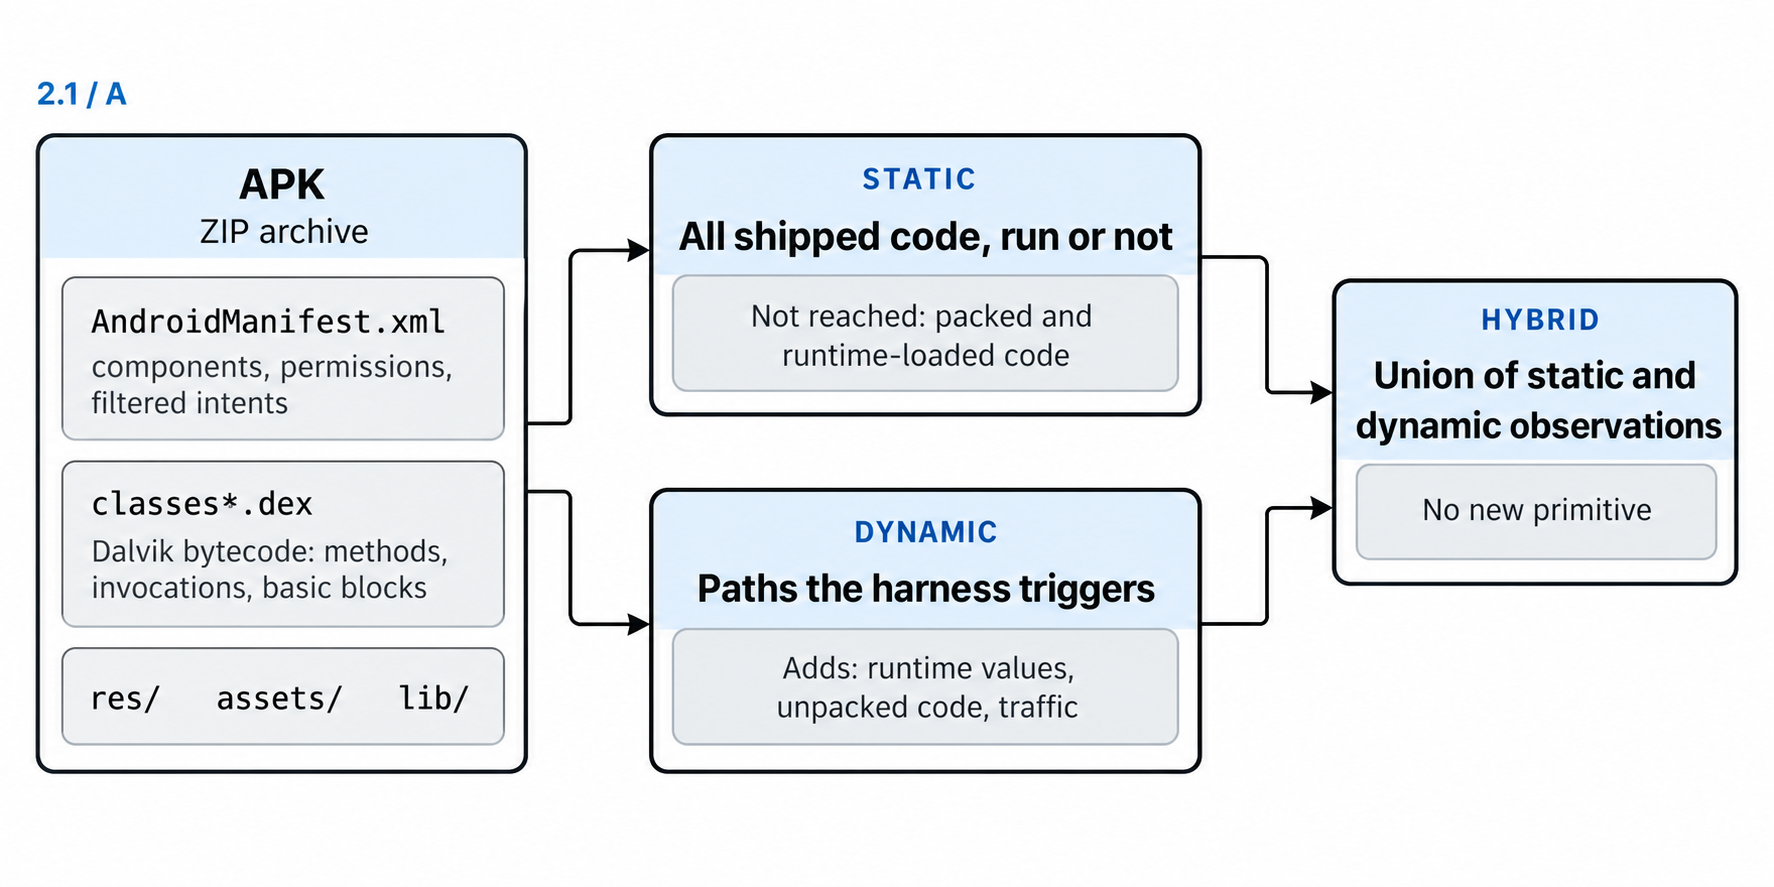
\includegraphics[width=\linewidth,trim=0 0 0 115bp,clip]
    {background-apk-analysis.png}
  \caption[Android package contents and analysis modes]{What an application package holds and
  what each mode of analysis reaches. Static observation covers all shipped code and not what
  the code does; dynamic observation covers what the code did, but only along the paths the
  harness triggered, and it alone reaches network traffic, which is the channel
  Chapter~\ref{chap:hybroid} uses. The graph objects built from the bytecode are named in
  Section~\ref{sec:background:graphs}.}
  \label{fig:background:apk}
\end{figure}

Static analysis reads the package and reasons about code that may never execute, which yields
coverage of everything shipped at modest computational cost. The engineering is mature.
Disassembly and call-graph construction are supplied by standard toolkits
\cite{desnos2012android, valleerai2010soot}, and taint analysis that models Android's component
lifecycle is available \cite{arzt2014flowdroid}. What no amount of engineering removes is a
ceiling on what static reasoning can decide. An adversary is able to construct obfuscation whose
analysis reduces to an NP-hard problem, which defeats semantics-aware static detection
\cite{moser2007limits}. That construction was demonstrated on x86 binaries, and the argument
carries to Dalvik by the same reasoning rather than having been shown there directly.

Dynamic analysis observes the application while it runs. Instrumentation ranges from taint
tracking on the device \cite{enck2014taintdroid} to whole-system emulation that reconstructs the
operating-system and Dalvik views together \cite{yan2012droidscope}. Traffic recorded during
execution is a further channel, and it is the one Chapter~\ref{chap:hybroid} uses. Two limits
apply throughout. Only the paths the harness triggers are observed, and an application may
detect the analysis environment and withhold the behaviour under investigation
\cite{petsas2014rage, vidas2014evading}.

Neither mode dominates the other. Measured under one protocol, static analysis proved at least
as effective as dynamic analysis, depending on how the applications were stimulated during
execution, while the combination of the two measured best \cite{onwuzurike2018family}. Hybrid
pipelines are consequently an established design \cite{lindorfer2015marvin}, and the question
Chapter~\ref{chap:hybroid} takes up is what such a combination buys on one set of samples under
a single protocol.

\subsection{Obfuscation, Packing, and Repackaging}
\label{sec:background:android:obfuscation}

Obfuscation is ordinary developer practice as much as attacker practice. Of 1.7 million free
applications on Google Play, 24.92 per cent had been obfuscated by their developers
\cite{wermke2018large}, and a measurement across 114,560 applications drawn from Google Play,
third-party markets and malware corpora found string encryption more frequent in malware and
packing more frequent outside Google Play \cite{dong2018understanding}. The effect on detection
is measurable. Three thousand benign and three thousand malicious applications, expanded into
73,362 obfuscated variants by 29 strategies, left most commercial anti-malware products severely
affected, and trivial transformations sufficed \cite{hammad2018large}. A later study of twelve
detectors found that none held its ideal-setting performance once obfuscation, concept drift and
adversarial examples were introduced \cite{gao2024comprehensive}.

Packing is a distinct mechanism and is kept separate here. A packed application ships an
encrypted original together with a wrapper that decrypts and loads it at runtime, so static
extraction fails outright instead of degrading. Commercial packers are used by malware authors,
and custom packers are written specifically to defeat the available unpackers
\cite{duan2018things}.

The packaging model also allows an attacker to graft a malicious rider onto a benign carrier
\cite{li2017understanding}. Applications produced this way are near-identical outside the
injected payload, and corpora assembled from them therefore contain duplicates. What those
duplicates cost depends on the task: the measured effect is limited for supervised
classification and substantially larger for unsupervised family clustering
\cite{zhao2021impact}. Section~\ref{sec:background:evaluation} returns to this as a problem of
evaluation rather than of extraction.

\section{Graph Representations of Programs}
\label{sec:background:graphs}

Representations are defined here, before the operators that learn over them. Two families are
needed. Chapters~\ref{chap:hybroid} and~\ref{chap:hgann} both derive a graph from program
structure, and Chapter~\ref{chap:hgann} then lifts that graph to a hypergraph. The notation
introduced in this section is the notation those chapters use, and neither redefines it.

\subsection{Control-Flow and Function-Call Graphs}
\label{sec:background:graphs:pairwise}

A \emph{control-flow graph} is a directed graph over the basic blocks of a single procedure. Its
vertices are maximal instruction sequences that contain no branch except possibly at the end,
and a directed edge records that control may pass from one block to the next. The object is
intra-procedural by definition \cite{bilot2024survey}. A \emph{call graph} takes the procedures
of a program as its vertices, with an edge from $f$ to $g$ recording that a call site in $f$ may
invoke $g$. It is inter-procedural, and a statically recovered call graph over-approximates,
since the analysis admits edges that no execution takes. For Android the call graph is taken at
method granularity over the recovered bytecode, and this dissertation calls that object a
\emph{function-call graph}: vertices are methods, and directed edges are method invocations
\cite{gascon2013structural, norouzian2025hgannmal}. The two objects are kept distinct throughout,
because their vertex sets and their edge semantics differ.

The two compose. Embeddings computed on per-method control-flow graphs may be attached to the
vertices of a function-call graph, which makes intra-procedural and inter-procedural structure
available together \cite{bilot2024survey}. Dropping the call edges from that composition leaves
a third object: a set of independently embedded control-flow graphs, pooled to application
level, with no invocation structure at all. The three are named here so that each contribution
chapter can state which of them it builds without introducing new machinery, and so that a
claim made about one is not read as a claim about another.

Whichever object is chosen, it is an artefact of the analyser rather than a property of the
program. Recovery depends on the toolkit and on how the component lifecycle is modelled
\cite{valleerai2010soot, arzt2014flowdroid, desnos2012android}, and abstracting call targets to
package or family level shrinks the vertex set at the cost of the callee's identity
\cite{onwuzurike2019mamadroid}. Vertex features may equally be learned rather than hand-built,
from the block structure of a procedure \cite{dai2016discriminative, xu2017neural} or from the
body of a method \cite{alon2019code2vec}.

\subsection{Hypergraphs and Higher-Order Relations}
\label{sec:background:graphs:hypergraphs}

A hypergraph $\mathcal{H} = (\mathcal{V}, \mathcal{E}, w)$ has a finite vertex set $\mathcal{V}$
and a family $\mathcal{E}$ of subsets of $\mathcal{V}$, each subset a hyperedge $e$ carrying a
weight $w(e) > 0$. Membership is recorded by the incidence matrix
$H \in \{0,1\}^{|\mathcal{V}| \times |\mathcal{E}|}$, where $h(v,e) = 1$ exactly when $v \in e$.
The degree of a vertex is $d(v) = \sum_{e \in \mathcal{E}} w(e)\, h(v,e)$ and the degree of a
hyperedge is $\delta(e) = \sum_{v \in \mathcal{V}} h(v,e) = |e|$. Writing $D_v$ and $D_e$ for the
diagonal matrices of vertex and hyperedge degrees and $W$ for the diagonal matrix of hyperedge
weights completes the apparatus \cite{zhou2006learning}. A graph is the special case in which
$\delta(e) = 2$ for every hyperedge, so every graph is a hypergraph and the converse fails.

An edge relates exactly two vertices, and encoding a group of several as a set of pairwise edges
loses the fact that its members belonged to one group. The projected graph cannot distinguish a
single hyperedge on three vertices from three separate pairwise relations among the same
vertices \cite{zhou2006learning}. Two projections are standard. \emph{Clique expansion} replaces
each hyperedge by the complete graph on its members, and \emph{star expansion} introduces a new
vertex per hyperedge joined to each member \cite{agarwal2006higherorder}.
Figure~\ref{fig:background:hypergraph} shows the hyperedge memberships and the information
lost in their pairwise projection.

\begin{figure}[tbp]
  \centering
  % Approved imagegen variant; trim removes only the temporary preview label.
  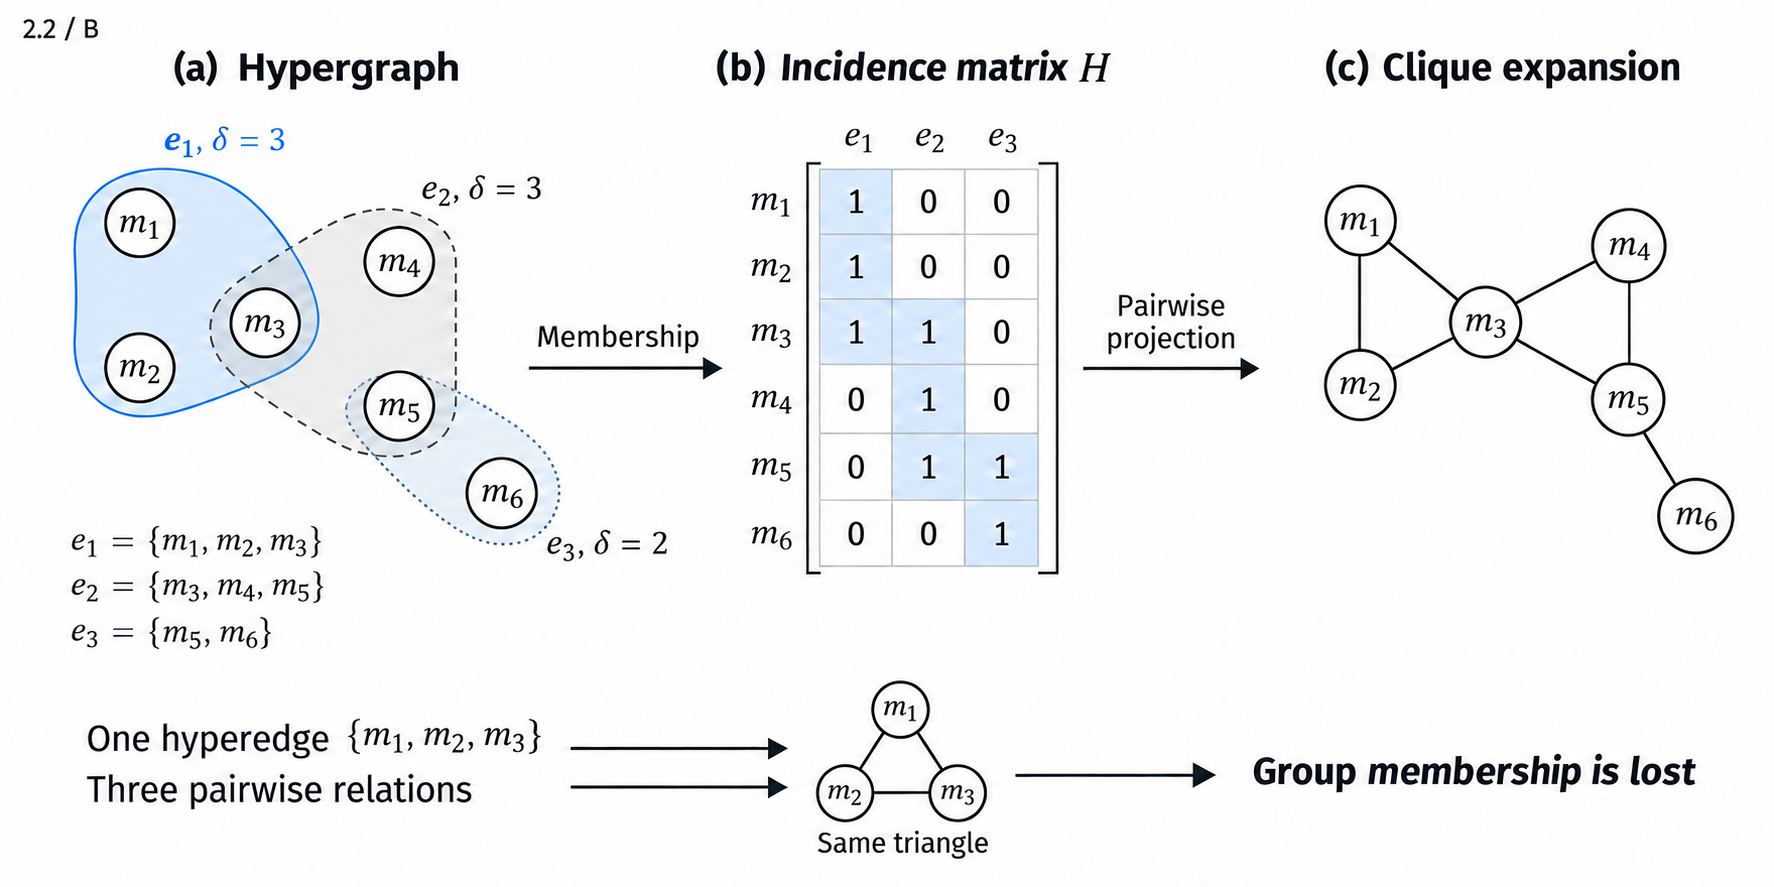
\includegraphics[width=\linewidth,trim=0 0 0 42bp,clip]
    {background-hypergraph-projection.png}
  \caption[Pairwise projection of a hypergraph]{The same six methods represented as
  (a) a hypergraph, (b) its incidence matrix $H$, and (c) its unweighted clique expansion.
  A matrix entry is one precisely when the method belongs to the corresponding hyperedge.
  Hyperedge $e_3$ joins two vertices and is therefore an ordinary graph edge. The lower
  example shows that the triangle over $m_1, m_2, m_3$ arises both from the single hyperedge
  $e_1$ and from three separate pairwise relations. The projection preserves pairwise
  adjacency but does not uniquely determine the original hyperedge memberships
  \cite{zhou2006learning}.}
  \label{fig:background:hypergraph}
\end{figure}

The sceptical reading of these definitions deserves stating, because it is the stronger position
to argue from. Agarwal et al.\ show that the hypergraph learning formulations of their period
reduce to the Laplacian of one expansion or the other, that the two coincide for uniform
hypergraphs, and that for non-uniform ones they differ only in how hyperedges of unequal size
are weighted; their conclusion is that graphs, not hypergraphs, lie at the heart of the problem
\cite{agarwal2006higherorder}. Chitra and Raphael sharpen the boundary. A random walk on a
hypergraph whose vertex weights do not vary between the hyperedges a vertex belongs to, the
\emph{edge-independent} case, is equivalent to a walk on a weighted clique expansion, so an
operator built on such a walk carries no higher-order information. Only \emph{edge-dependent}
vertex weights escape the equivalence \cite{chitra2019randomwalks}.

What the projection costs has since been measured rather than asserted. An evaluation framework
that expands, learns and then reconstructs reports depressed performance at vertex, hyperedge
and hypergraph level across eight datasets \cite{kang2024low}; two recurring hyperedge patterns
have been identified as the source of the loss in every projection, together with a
combinatorial impossibility result on recovering the discarded structure \cite{wang2024graphs};
and an expressivity hierarchy names the invariants a clique expansion cannot represent
\cite{jiang2026widthwall}. Section~\ref{sec:background:learning} describes the operators built on
this apparatus, and Chapter~\ref{chap:hgann} develops the one it uses.

\section{Learning over Graphs}
\label{sec:background:learning}

The operators described here learn representations over a structure whose construction was
fixed in Section~\ref{sec:background:graphs}. Three families are relevant: neighbourhood
aggregation on pairwise graphs, attention-weighted aggregation, and convolution over an
incidence structure. This section states what each does and what is known about its limits. The
notation stays as defined above, and the operator Chapter~\ref{chap:hgann} builds on is
developed there rather than here.

\subsection{Message Passing}
\label{sec:background:learning:messagepassing}

Most graph neural networks share one scheme. Each vertex holds a state, that state is updated
from the states of its neighbours by a permutation-invariant aggregation, and the update is
applied for a fixed number of rounds \cite{gilmer2017neural}. The convolutional instance fixes
the aggregation coefficients in advance from the degrees of the two endpoints, so a vertex
combines its neighbours in proportions that the graph determines and training does not alter
\cite{kipf2017semi}.

Two limits on this family are established. The first is a bound on what it can tell apart: no
network in the family distinguishes two graphs that one-dimensional Weisfeiler-Leman colour
refinement assigns the same colours, and an architecture reaching that bound is as
discriminative as the scheme permits \cite{xu2019powerful}. The second concerns depth. Repeated
propagation drives the representations within a connected component towards one another, so
adding rounds to widen a vertex's receptive field costs discriminability between vertices
\cite{li2018deeper}. Both bear on program graphs, where the structures compared are often large
and locally similar.

\subsection{Attention}
\label{sec:background:learning:attention}

Attention replaces fixed coefficients with learned ones. A scoring function is applied to each
vertex and its neighbour, the scores across a neighbourhood are normalised, and the resulting
weights determine the combination \cite{velickovic2018graph}; the mechanism was introduced for
sequences before it was carried to graphs \cite{vaswani2017attention}. The motivation is that
some neighbours matter more than others, and that which ones matter should be learned rather
than read off the degree.

Three results qualify that motivation, and they should be kept apart. Brody et al.\ show that
the ranking the standard formulation induces over a vertex's neighbours is the same for every
query vertex, so the mechanism selects globally important neighbours rather than neighbours
important to a particular vertex; a revised scoring function removes the restriction
\cite{brody2022gatv2}. Fang et al.\ bound both scoring functions, the linear form used by the
original mechanism and the multi-layer form introduced by its revision, showing that each
realises only finitely many neighbour rankings at bounded width and depth \cite{fang2025kaa}.
The same work reports that on node-property benchmarks over pairwise graphs, evaluated with
GCN, GraphSAGE and GIN as non-attentive baselines, no unmodified attentive model outperformed
all of those baselines on any dataset or task \cite{fang2025kaa}. The defensible reading of that
last result is negative about the evidence rather than about the mechanism: an advantage for
attention over fixed aggregation has not been demonstrated on those benchmarks, and the
expressive power of the standard scoring functions is bounded.

Whether either finding transfers to operators defined over hyperedges is not established in the
literature, since both analyses concern pairwise operators. Section~\ref{sec:hgann:8} shows that
the static-ranking argument carries over to the additive hyperedge score used there. For other
scoring functions over hyperedges, and for the finite-ranking bound, the question is open, and
Section~\ref{sec:background:learning:hypergraphconvolution} returns to it.

A methodological point follows, and it concerns how such architectures are designed rather than
how they perform. Where a model changes its relational encoding and its aggregation weighting at
the same time, the contribution of each change cannot be recovered from the reported totals. The
two have to be varied separately for either to be attributed.

\subsection{Hypergraph Convolution}
\label{sec:background:learning:hypergraphconvolution}

Operators over a hypergraph propagate in two stages. Signal moves from the vertices to the
hyperedges that contain them, is combined at each hyperedge, and returns to the member vertices,
with the incidence structure and the degree matrices of
Section~\ref{sec:background:graphs:hypergraphs} supplying the normalisation
\cite{feng2019hypergraph, gao2023hgnn}. Two design routes exist. One reduces the hypergraph to a
graph and applies a pairwise operator to the result \cite{yadati2019hypergcn}, which inherits
the losses recorded in Section~\ref{sec:background:graphs:hypergraphs}; the other treats a
hyperedge as a multiset and learns the functions that aggregate it
\cite{chien2022allset}. Attention has been carried across to this setting by making the
incidence structure itself learnable, so that membership is weighted by a real value instead of
a binary indicator \cite{bai2021hypergraphattention}.

Three observations bound what is known. Standard hypergraph convolution averages over the
members of a hyperedge and therefore attenuates variation between them, a low-pass bias whose
discarded high-frequency component has been characterised \cite{li2026highpass}. The operator
most widely used has since been superseded by a stability-oriented successor from its own
authors \cite{gao2026hgnnv2}, which is the reference point for any claim about its limitations.
No theoretical analysis of attention scoring in hypergraph operators has appeared since 2024;
the nearest treatments predate that, in work on equivariant hypergraph networks and on
generalising set transformers to hypergraphs \cite{kim2022equivariant, kim2021transformers}. The
transfer question raised in Section~\ref{sec:background:learning:attention} therefore remains
open on the theoretical side as well as the empirical one.

\section{Detection in Networked and Cyber-Physical Systems}
\label{sec:background:networks}

This section covers the unit of observation used in network detection, the families of method
defined over it, the particular character of industrial and IoT deployments, and the corpora on
which results are reported. Chapter~\ref{chap:anomaly} draws on it, although the Android
material precedes it for the reason given at the head of this chapter.

\subsection{Network Flows as a Unit of Observation}
\label{sec:background:networks:flows}

Detection at the flow level summarises the packets sharing a five-tuple into counts, durations
and byte totals. Working at that level lowers processing cost and survives payload encryption,
at the price of discarding content \cite{sperotto2010overview}. Network intrusion detection is
conventionally divided into signature matching against descriptions of known attacks and
anomaly detection against a learned model of normal behaviour \cite{paxson1999bro}, and the
second is what the rest of this section concerns. Section~\ref{sec:hybroid:7} states the
particular flow feature set Chapter~\ref{chap:hybroid} uses, rather than drawing it from here.

\subsection{Anomaly-Detection Method Families}
\label{sec:background:networks:families}

Anomalies are conventionally classed as point, contextual or collective, and detectors differ in
whether labels are available for both classes, for one, or for neither
\cite{chandola2009anomaly}. Classical methods score a point by the local density around it
\cite{breunig2000lof} or by how few partitions are needed to isolate it
\cite{liu2008isolation}. Deep detectors replace a hand-built feature space with a learned one,
and the shallow and deep families admit a common formulation \cite{ruff2021unifying,
pang2021deep}. Where the data are relational, the anomaly is a property of structure rather than
of any single record, and the object flagged may be a vertex, an edge or a subgraph
\cite{akoglu2015graph}. That observation is what connects this section to
Section~\ref{sec:background:graphs}.

The security setting resists the standard formulation. The cost of a false alarm is high,
network traffic is more variable than a model of normal behaviour admits, and data adequate for
evaluation are scarce \cite{sommer2010outside}.

\subsection{Communication Structure in Industrial and IoT Networks}
\label{sec:background:networks:industrial}

Industrial and IoT traffic is comparatively regular, because the devices are few and their
interactions are prescribed by the process under control. A whitelist of permitted communication
relations is therefore a workable model of normal behaviour. Barbosa et al.\ built such
whitelists in SCADA networks from four packet properties and reported both that the whitelists
stabilise and that rare legitimate flows continue to raise false positives
\cite{barbosa2013flow}; Yoon and Ciocarlie modelled communication patterns per host pair for the
same purpose \cite{yoon2014communication}. Neither of the two ideas that follow from this
originates with service-oriented deployments. Scoring behaviour against a graph of which host
talks to which was established for carrier traffic \cite{iliofotou2007network,
jin2009unveiling}, and the dependency graph between services was already being recovered
automatically from passively observed traffic in enterprise networks \cite{bahl2007towards,
chen2008automating, natarajan2012nsdminer}.

Where the system is cyber-physical, the observation may be the process rather than the traffic,
and detectors are then fitted to sensor and actuator series recorded from testbeds
\cite{mathur2016swat, kravchik2018detecting}. In IoT deployments the unit modelled is often the
individual device. Models of that kind hold under the conditions they were fitted to and lose a
substantial part of their measured performance when the deployment changes: reproduced figures
fall by roughly a quarter to a half beyond three months, and by a comparable margin between test
sites \cite{maali2025evaluating}.

\subsection{Datasets and Measurement Limits}
\label{sec:background:networks:datasets}

The corpora this field reports on are known to be defective. KDD~99 was shown to contain
redundant records that bias measured accuracy \cite{tavallaee2009nslkdd}, and a later audit of
CICIDS2017, UNSW-NB15 and comparable sets catalogues construction faults that allow trivial
features to separate attack traffic from benign \cite{flood2024bad}. Two further limits bear on
any figure reported here. Detectors reporting detection rates above 99 per cent have been shown
to be trained and tested on the same attack type, with performance not surviving attack types
absent from training \cite{kus2022false}. And when 70 published approaches were re-run on one
evaluation platform, four deliberately simple tests on process values, using minima, maxima and
rate of change, performed on par with them \cite{wolsing2022simple}.
Section~\ref{sec:background:evaluation} treats the protocol-level causes.

\section{Adversarial Machine Learning}
\label{sec:background:adversarial}

Chapter~\ref{chap:introduction} has already set out what the record shows about published
defences. This section supplies the vocabulary that account assumed, and it is the vocabulary
Chapters~\ref{chap:hybroid}, \ref{chap:hgann} and~\ref{chap:advml} use to state what they claim
and what they do not.

\paragraph{Threat models.} A threat model states four things: the attacker's goal, the
attacker's knowledge of the system, the attacker's capability to act on it, and the constraints
on what may be modified \cite{biggio2014security, vassilev2025adversarial}. A claim about an
attack or about robustness cannot be interpreted without all four \cite{carlini2019evaluating}.
Knowledge is conventionally divided into three levels. Under \emph{white box} the attacker knows
the training data, the feature representation, the learning algorithm, the trained parameters
and any deployed defence \cite{biggio2018wildpatterns}. Under \emph{black box} the attacker
knows neither parameters nor architecture and interacts through the prediction interface, either
by transferring from a substitute model trained on its outputs or by searching directly with
queries \cite{papernot2017practical}. \emph{Grey box} lies between the two: some components of
the white-box list are known and training cannot be influenced. Because the term is used
inconsistently in the literature, every use in this dissertation names which components the
attacker is assumed to know. One limit on the taxonomy should be recorded with it. A survey of
271 practitioners found that the knowledge assumptions of academic threat models are more
generous to the attacker than deployment conditions usually allow \cite{grosse2024towards}.

\paragraph{Classes of attack.} \emph{Evasion} modifies an input at test time so that a trained
model misclassifies it, leaving the model unchanged \cite{biggio2013evasion}. \emph{Poisoning}
manipulates the training data or the training process so that the resulting model is degraded or
carries behaviour the attacker chose \cite{biggio2012poisoning, jagielski2018manipulating}, and
the \emph{backdoor} is its sub-case, in which the implanted behaviour is conditioned on a trigger
\cite{gu2019badnets}. Confidentiality attacks form a third class: a functional copy of a
deployed model can be recovered through its prediction interface \cite{tramer2016stealing}. The
word adversarial covers all three and is not a synonym for evasion.

\paragraph{Feature space and problem space.} A \emph{feature-space} attack perturbs the feature
vector directly, with no requirement that any real input maps to the result. A
\emph{problem-space} attack modifies the artefact itself and must satisfy four constraints: the
transformation has to be available, semantics have to be preserved, the result has to be
plausible, and it has to survive preprocessing. Moving between the two is the inverse
feature-mapping problem, and in the malware setting the modified sample must still install and
still run \cite{pierazzi2020intriguing}. The distinction is load-bearing for
Chapters~\ref{chap:hybroid} and~\ref{chap:hgann}, because attacks on static Android detectors
operate at code level, upstream of feature extraction, so a representation derived from that
extraction inherits the attacker's influence whatever the learning architecture
\cite{song2026fcghunter}. Which operators reach which representation depends on what is
extracted, and each chapter settles that where it states its threat model. Early work on
Android established the feature-space case \cite{grosse2017adversarial}.

\paragraph{Adaptive attacks and robustness.} An \emph{adaptive} attack is constructed in
knowledge of the defence and tuned against that specific defence, in contrast to a fixed attack
applied unchanged \cite{tramer2020adaptive}. The recurring reason a defence appears to hold and
does not is gradient masking, where the defence obstructs the optimisation an attack relies on
without reducing the attacker's reach \cite{athalye2018obfuscated}. \emph{Robustness} is
therefore defined relative to a stated threat model and a stated attack budget. It is a property
of the pair, never of a model alone, and a robustness figure reported without those parameters
cannot be compared with another \cite{carlini2019evaluating}. Gradient-based attacks at fixed
perturbation budgets \cite{goodfellow2015explaining, madry2018pgd} are the reference instruments
against which the defences of Chapter~\ref{chap:advml} are measured.

\section{Performance Measures and Evaluation Methodology}
\label{sec:background:evaluation}

This section defines the measures used in Chapters~\ref{chap:anomaly} to~\ref{chap:advml}, with
explicit observation units and aggregation rules. Dimensionless scores are proportions:
$m$ corresponds to $100m$ per cent, and $m_1-m_2$ to $100(m_1-m_2)$ percentage points.

\subsection{Observation Units and Confusion Counts}
\label{sec:background:metrics:counts}

Let $\mathcal D=\{(x_i,y_i)\}_{i=1}^{N}$ be a labelled evaluation set with $N>0$, and let
$\widehat y_i=h(x_i)$ be the prediction of a fitted classifier. For a single-label task with
class set $\mathcal Y$, the confusion matrix $\mathbf C$ records true labels in its rows and
predicted labels in its columns:
\begin{equation}
  C_{ab}=\sum_{i=1}^{N}\mathbf1\{y_i=a,\ \widehat y_i=b\},
  \qquad a,b\in\mathcal Y.
  \label{eq:background:confusion}
\end{equation}
In binary detection, $1$ denotes an attack or malware and $0$ denotes normal or benign behaviour. With both axes
ordered as $(0,1)$,
\begin{equation}
  \mathbf C_{\mathrm{bin}}=
  \begin{pmatrix}\mathrm{TN}&\mathrm{FP}\\\mathrm{FN}&\mathrm{TP}\end{pmatrix},
  \qquad N=\mathrm{TP}+\mathrm{TN}+\mathrm{FP}+\mathrm{FN}.
  \label{eq:background:binary-confusion}
\end{equation}
True positives and true negatives are correct decisions. A false positive flags a negative
observation; a false negative misses a positive observation \cite{fawcett2006roc}.

The S7-300 evaluation counts network records, SWaT counts timestamps, and the Android studies
count applications. Timestamp metrics give longer attacks more weight; episode-level assessment
requires a separate matching rule and denominator \cite{sorbo2024navigating}. Collapsing attack
types into one positive class turns errors between those types into correct binary detections
(Section~\ref{sec:anomaly:iuno-results}).

\subsection{Binary Detection Measures and Class Prevalence}
\label{sec:background:metrics:binary}

Accuracy $A$ is the fraction of all observations classified correctly. Precision $P$ is the
fraction of positive predictions that are correct, whereas recall $R$ is the fraction of
positive observations detected:
\begin{equation}
  A=\frac{\mathrm{TP}+\mathrm{TN}}{N},\qquad
  P=\frac{\mathrm{TP}}{\mathrm{TP}+\mathrm{FP}},\qquad
  R=\frac{\mathrm{TP}}{\mathrm{TP}+\mathrm{FN}}.
  \label{eq:background:accuracy-precision-recall}
\end{equation}
Recall is also called sensitivity or the true-positive rate (TPR). The $F_1$ score combines
precision and recall through their harmonic mean:
\begin{equation}
  F_1=\frac{2\mathrm{TP}}{2\mathrm{TP}+\mathrm{FP}+\mathrm{FN}},\qquad
  H(P,R)=\frac{2PR}{P+R}=F_1
  \quad\text{when the ratios are defined}.
  \label{eq:background:f1}
\end{equation}
The count form omits true negatives and gives $F_1=0$ when $\mathrm{TP}=0$ and
$\mathrm{FP}+\mathrm{FN}>0$. We use the continuous extension $H(0,0)=0$ when both defined rates
are zero
\cite{fawcett2006roc,sorbo2024navigating}.

False-positive and false-negative rates (FPR and FNR) measure class-conditional errors.
Specificity, or true-negative rate (TNR), complements FPR; balanced accuracy averages the two class recalls
\cite{fawcett2006roc,grandini2020metrics}:
\begin{equation}
  \begin{aligned}
    \mathrm{FPR}&=\frac{\mathrm{FP}}{\mathrm{FP}+\mathrm{TN}},
    &\mathrm{TNR}&=\frac{\mathrm{TN}}{\mathrm{TN}+\mathrm{FP}}=1-\mathrm{FPR},\\
    \mathrm{FNR}&=\frac{\mathrm{FN}}{\mathrm{TP}+\mathrm{FN}}=1-R,
    &\mathrm{BAcc}&=\frac{R+\mathrm{TNR}}{2}.
  \end{aligned}
  \label{eq:background:error-rates}
\end{equation}
The false fraction among positive predictions is $1-P=\mathrm{FP}/(\mathrm{TP}+\mathrm{FP})$,
with a different denominator from FPR. Zero denominators make ratios undefined unless an
explicit replacement or exclusion rule is given.

Let $\pi=(\mathrm{TP}+\mathrm{FN})/N$ be the positive-class prevalence. Writing precision and
accuracy in terms of the class-conditional rates gives
\begin{equation}
  \begin{aligned}
    P(\pi)&=\frac{\pi\,\mathrm{TPR}}
      {\pi\,\mathrm{TPR}+(1-\pi)\,\mathrm{FPR}},\\
    A(\pi)&=\pi\,\mathrm{TPR}+(1-\pi)\,\mathrm{TNR}.
  \end{aligned}
  \label{eq:background:prevalence}
\end{equation}
Bayes' rule gives the precision identity \cite{axelsson2000base}. Varying $\pi$ at fixed TPR
and FPR gives a conditional prevalence-sensitivity calculation (Section~\ref{sec:hgann:10}).
Balanced accuracy removes the explicit prevalence weights, but changes in class-conditional
data distributions can still change both recalls.

\subsection{Multiclass and Multilabel Aggregation}
\label{sec:background:metrics:aggregation}

For $K$ mutually exclusive classes indexed by $1,\ldots,K$, let $n_k=\sum_b C_{kb}$ be the support of class $k$ and
$\pi_k=n_k/N$. A one-versus-rest calculation treats class $k$ as positive and all other classes
as negative:
\begin{equation}
  \begin{aligned}
    \mathrm{TP}_k&=C_{kk},
    &\mathrm{FN}_k&=n_k-C_{kk},\\
    \mathrm{FP}_k&=\sum_a C_{ak}-C_{kk},
    &\mathrm{TN}_k&=N-\mathrm{TP}_k-\mathrm{FP}_k-\mathrm{FN}_k.
  \end{aligned}
  \label{eq:background:one-vs-rest}
\end{equation}
The binary definitions then give $P_k$, $R_k$ and $F_{1,k}$. For any of these measures $M_k$,
macro averaging assigns equal class weights, while support-weighted averaging assigns weights
proportional to class size:
\begin{equation}
  M_{\mathrm{macro}}=\frac1K\sum_{k=1}^{K}M_k,
  \qquad
  M_{\mathrm{weighted}}=\sum_{k=1}^{K}\pi_k M_k.
  \label{eq:background:class-averages}
\end{equation}
Multiclass balanced accuracy is $R_{\mathrm{macro}}$. S7-300 results report both macro and
weighted $F_1$ to account for the dominant normal class. A high macro average does not establish
uniform per-class performance.

Micro averaging instead pools the one-versus-rest counts before calculating a ratio
\cite{grandini2020metrics}:
\begin{equation}
  P_{\mathrm{micro}}=
  \frac{\sum_k\mathrm{TP}_k}{\sum_k(\mathrm{TP}_k+\mathrm{FP}_k)},\qquad
  R_{\mathrm{micro}}=
  \frac{\sum_k\mathrm{TP}_k}{\sum_k(\mathrm{TP}_k+\mathrm{FN}_k)}.
  \label{eq:background:micro-averages}
\end{equation}
Micro $F_1$ uses the same count formula as Equation~\ref{eq:background:f1}, after summing over
classes. With one true and one predicted label per observation and all classes included,
both denominators in Equation~\ref{eq:background:micro-averages} equal $N$. With defined class
recalls, or an explicit zero-fill convention for classes of zero support, this gives
\begin{equation}
  P_{\mathrm{micro}}=R_{\mathrm{micro}}=F_{1,\mathrm{micro}}
  =R_{\mathrm{weighted}}=A=\frac{\operatorname{tr}(\mathbf C)}{N}.
  \label{eq:background:micro-identity}
\end{equation}
Opitz and Burst distinguish the mean of class $F_1$ scores from the harmonic mean of macro
precision and recall
\cite{opitz2019macrof1}. For defined class ratios,
\begin{equation}
  F_{1,\mathrm{macro}}
  =\frac1K\sum_k H(P_k,R_k)
  \leq H(P_{\mathrm{macro}},R_{\mathrm{macro}})
  \leq\frac{P_{\mathrm{macro}}+R_{\mathrm{macro}}}{2}.
  \label{eq:background:macro-f1}
\end{equation}
Here, macro $F_1$ denotes the mean of class scores. Unspecified source conventions remain
unresolved in Chapters~\ref{chap:hybroid} and~\ref{chap:hgann}. Reporting must identify the class
set and any zero-denominator policy.

Always predicting class $k$ gives accuracy $\pi_k$, while $\max_k\pi_k$ is the empirical
majority-class reference. A deployable baseline must choose its label before test evaluation,
for example from training labels, and may not match the test majority.

Multilabel prediction assigns several binary labels to each observation. In the facial-attribute
task, $y_i,\widehat y_i\in\{0,1\}^{J}$ and the reported accuracy averages individual label
decisions:
\begin{equation}
  A_{\mathrm{attr}}=\frac1{NJ}\sum_{i=1}^{N}\sum_{j=1}^{J}
    \mathbf1\{\widehat y_{ij}=y_{ij}\}.
  \label{eq:background:attribute-accuracy}
\end{equation}
Chapter~\ref{chap:advml} uses $J=40$ \cite{sparta2022d76}. Each attribute decision contributes
separately; the score does not require all labels of an image to be correct.

\subsection{ROC Curves and Area under the Curve}
\label{sec:background:metrics:roc}

For scores $s_i$ whose larger values favour the positive class, thresholding gives
$\widehat y_i(\tau)=\mathbf1\{s_i\geq\tau\}$. Varying $\tau$ traces the receiver operating
characteristic (ROC) points $(\mathrm{FPR}(\tau),\mathrm{TPR}(\tau))$
\cite{fawcett2006roc}. With $r(u)$ the linearly interpolated TPR at FPR $u$, the empirical area
under the curve (AUC) is
\begin{equation}
  \begin{aligned}
    \mathrm{AUC}&=\int_0^1 r(u)\,\mathrm du\\
    &=\frac1{N_+N_-}\sum_{i:y_i=1}\sum_{j:y_j=0}
      \left[\mathbf1\{s_i>s_j\}+\frac12\mathbf1\{s_i=s_j\}\right],
  \end{aligned}
  \label{eq:background:auc}
\end{equation}
where $N_+,N_->0$ count positive and negative observations. AUC measures positive--negative pair ranking,
with half credit for ties. Perfect and independent random rankings give one and expected
$0.5$, respectively. One confusion matrix gives only an operating point; AUC specifies neither
a deployment threshold nor probability calibration.

Multiclass one-versus-rest curves compare each class with the remainder. Unweighted macro AUC
is $K^{-1}\sum_k\mathrm{AUC}_k$; other weighting or curve-averaging conventions must be stated
\cite{fawcett2006roc}. \hybroid{} reports per-class ROC AUC (Chapter~\ref{chap:hybroid}).

\subsection{Performance under Adversarial Input}
\label{sec:background:metrics:adversarial}

An adversarial performance measure requires a fixed threat model and valid perturbed inputs
\cite{carlini2019evaluating}. For an attack $a$ applied to matched, single-label observations,
let $A_{\mathrm{clean}}$ be the clean accuracy and define
\begin{equation}
  A_a=\frac1N\sum_{i=1}^{N}\mathbf1\{h(a(x_i))=y_i\},
  \qquad \Delta_a=A_{\mathrm{clean}}-A_a.
  \label{eq:background:accuracy-loss}
\end{equation}
The SAFAIR score in Chapter~\ref{chap:advml} uses this signed accuracy difference
\cite{sparta2022d76}. For the attribute task, Equation~\ref{eq:background:attribute-accuracy}
supplies both terms. Report clean and attacked accuracy alongside the loss: equal differences
can occur at different levels of classification performance.

Attack success measures attainment of a specified goal. One explicit convention restricts
evaluation to initially correct examples, $I_{\mathrm{corr}}=\{i:h(x_i)=y_i\}$. For target
labels $t_i$, let $I_t=\{i\in I_{\mathrm{corr}}:t_i\neq y_i\}$. Conditional untargeted and
targeted attack-success rates are then
\begin{equation}
  \begin{aligned}
    \mathrm{ASR}_{\mathrm{untargeted}}
      &=\frac1{|I_{\mathrm{corr}}|}\sum_{i\in I_{\mathrm{corr}}}
        \mathbf1\{h(a(x_i))\neq y_i\},\\
    \mathrm{ASR}_{\mathrm{targeted}}
      &=\frac1{|I_t|}\sum_{i\in I_t}\mathbf1\{h(a(x_i))=t_i\}.
  \end{aligned}
  \label{eq:background:attack-success}
\end{equation}
Report eligible-set sizes and any alternative eligibility rule; empty sets give undefined rates.
These goal-specific rates differ from $\Delta_a$. Chapter~\ref{chap:advml} develops attribute
criteria and per-example attack-suite aggregation as analytical measures, not recovered contest
scores. Finite attacks do not certify worst-case robustness
\cite{carlini2019evaluating}.

\subsection{Aggregation and Operational Reporting}
\label{sec:background:metrics:reporting}

Let $M_b$ be a metric from fold or run $b$. Its mean and sample standard deviation are
\begin{equation}
  \overline M=\frac1B\sum_{b=1}^{B}M_b,
  \qquad
  s_M=\sqrt{\frac1{B-1}\sum_{b=1}^{B}(M_b-\overline M)^2},\qquad B>1.
  \label{eq:background:run-aggregation}
\end{equation}
Fold averaging can differ from calculating $M(\sum_b\mathbf C^{(b)})$ on pooled counts,
especially for nonlinear measures such as $F_1$. Class and fold averaging must be specified
separately. \hybroid{} reports five-fold means without the values needed for $s_M$.
Confidence intervals additionally require a sampling model that accounts for dependence;
correlated timestamps are not independent repetitions \cite{sorbo2024navigating}.

Operational performance uses time and resource denominators. For an observation interval of
duration $T$, let $n_{\mathrm{in}}$, $n_{\mathrm{proc}}$ and $n_{\mathrm{drop}}$ count input,
processed and dropped frames. The extractor measurements in Chapter~\ref{chap:anomaly} use
\begin{equation}
  q_{\mathrm{in}}=\frac{n_{\mathrm{in}}}{T},\qquad
  q_{\mathrm{proc}}=\frac{n_{\mathrm{proc}}}{T},\qquad
  p_{\mathrm{drop}}=\frac{n_{\mathrm{drop}}}{n_{\mathrm{in}}}.
  \label{eq:background:throughput}
\end{equation}
Using seconds gives frame rates per second. Chapter~\ref{chap:anomaly} also reports mean
whole-device CPU utilisation and peak memory. Its 95th-percentile delay from window close to
record emission excludes acquisition time; service-graph latency measures inter-service round trips. Timing endpoints
and summary statistics must be stated before comparison.

Two further ratios describe operational scope:
\begin{equation}
  r_{\mathrm{FA}}=\frac{n_{\mathrm{false\ alarm\ episodes}}}{T_{\mathrm{benign}}},
  \qquad
  c_{\mathrm{proc}}=\frac{N_{\mathrm{analysed}}}{N_{\mathrm{source}}}.
  \label{eq:background:alarm-coverage}
\end{equation}
The episode rate requires a grouping rule and benign exposure in a stated time unit; record FPR
alone cannot determine it. Processing coverage gives the analysed fraction of source applications.
Classification scores exclude the remaining applications, as in \hybroid{}. Complexity bounds
in Chapter~\ref{chap:hgann} describe scaling under stated assumptions, rather than measured
runtime or memory use.

\subsection{Experimental Protocol and Bias}
\label{sec:background:evaluation:bias}

Metric definitions fix the quantities calculated from an evaluation. The following considerations
concern how the data and protocol determine which conclusions those quantities support.

\paragraph{Sampling bias in space and time.} \emph{Temporal bias} is a split that allows a model
to learn from samples postdating the ones it is tested on, which reports a figure no deployment
reproduces. \emph{Spatial bias} is a test set whose composition differs from the deployment,
which leaves precision uninterpretable. A sound evaluation constrains both: training data must
precede test data, and the ratio between classes in the test set must reflect the setting the
system is claimed for \cite{pendlebury2019tesseract}. Drift is the mechanism that makes a
randomly ordered split optimistic \cite{jordaney2017transcend}. Curation of the corpus decides
as much as the split does, and guidance published since those constraints were formalised
revises parts of them \cite{chow2025beyond, kan2024tesseract}.

\paragraph{Leakage.} Any transformation fitted before the split moves information from the test
set into training. Resampling, feature selection, normalisation and model selection all have
this property when applied to the whole corpus, and the resulting figure measures the procedure
rather than the model \cite{arp2022dos}. Duplicate and near-duplicate samples are a second
channel, since repackaging produces applications that differ only in the injected payload and
copies of one application may fall on both sides of the split. The measured cost is uneven:
limited for supervised classification, and substantially larger for unsupervised family
clustering \cite{zhao2021impact, irolla2018duplication}.

\paragraph{Event definitions and benchmark labels.} In time-series detection,
\emph{point adjustment} marks an entire anomalous window as detected once
any single point inside it is flagged, which inflates F1 to the point that randomly generated
scores outperform published detectors \cite{kim2022towards, sorbo2024navigating}. Some standard
benchmarks also contain mislabelled or trivially separable anomalies, so a high score on them is
weak evidence \cite{liu2024elephant}.

\paragraph{Baselines and adaptive evaluation.} A reported gain is not established until a simple
baseline has been run under the same protocol. Where that has been done, the gap has often
disappeared: re-implementing eight provenance-based intrusion detectors in one framework left a
simple neural network matching the state of the art on most of the datasets tested
\cite{bilot2025sometimes}. For a defence the corresponding rule concerns the attack. A
robustness claim is bounded by the strongest attack applied to it, so the defence has to be
evaluated against an attack adapted to it \cite{carlini2019evaluating}, and defences evaluated
only by their own authors have repeatedly failed under adapted attacks
\cite{athalye2018obfuscated, tramer2020adaptive}.

\paragraph{The standard adopted here.} Every empirical chapter of this dissertation states its
split policy and uses time-aware splits where the timestamps permit, reports the class ratio
alongside any aggregate score, reports no point-adjusted figure, places a trivial baseline beside
each headline result, and states preprocessing and random seeds \cite{daoudi2021lessons}. Results
carried over from the source publications cannot be retrofitted to all of this, and each chapter
says in its Limitations which parts were not met.

\section{Summary and Research Gaps}
\label{sec:background:summary}

Three threads run through the preceding sections. The first concerns what an analysis system is
able to observe. An Android package exposes a manifest and bytecode to static reading, exposes
executed behaviour and recorded traffic to dynamic instrumentation, and neither mode dominates
the other. Network deployments expose flows, and industrial and IoT systems additionally expose
process values and a comparatively regular pattern of who communicates with whom. The second
thread concerns how those observations are structured. Program behaviour is encoded as
control-flow and function-call graphs, communication as graphs over hosts or services, and both
may be lifted to hypergraphs when a relation holds among more than two elements. The operators
that learn over these structures are bounded in what they can distinguish, and the projection
from a hypergraph back to a graph discards information that has now been measured. The third
thread concerns measurement. Reported performance depends on the split, on the corpus, on the
baseline it is compared against, and, where a defence is claimed, on the strength of the attack
applied to it.

Four questions are left open by this material, and each is taken up by one of the research
questions stated in Section~\ref{sec:intro:rqs}.

\phantomsection
\paragraph{G1. How behaviour in networked and industrial systems should be represented as
deployments change.}\label{gap:1}
Communication whitelists, service-dependency graphs, flow records, and process time series have
each supported anomaly detection under the conditions in which they were fitted
\cite{barbosa2013flow,yoon2014communication,goh2016swatdataset}. The evidence is split across
different observation units and system assumptions, and traffic-based models lose a substantial
part of their measured performance once a deployment moves in time or place
\cite{maali2025evaluating}. The literature lacks a common account of how these representation
choices support detection as the observed system changes. RQ1 takes up the question through
communication graphs and modular analysis of network and process features.

\phantomsection
\paragraph{G2. The value of combining program structure with observed behaviour.}\label{gap:2}
MARVIN and the study by Onwuzurike et al.\ report benefits from combining static and dynamic
features in within-system comparisons \cite{lindorfer2015marvin, onwuzurike2018family}.
Those results concern particular observation types and prediction tasks. Whether the benefit
persists when either changes requires comparison of the fused representation with each
modality alone on the same samples. RQ2 investigates this question for program-graph and
network-flow features in binary detection and malware-category classification.

\phantomsection
\paragraph{G3. Whether higher-order representation of program structure pays for itself.}\label{gap:3}
Program structure is represented pairwise, and a relation holding among several functions at
once is flattened into a set of edges that cannot record it as one group
\cite{zhou2006learning}. Hypergraphs remove the restriction and the cost of the projection has
been quantified \cite{kang2024low, wang2024graphs}, yet the sceptical result also stands: an
operator whose vertex weights do not vary between the hyperedges a vertex belongs to is
equivalent to one acting on a weighted clique expansion \cite{agarwal2006higherorder,
chitra2019randomwalks}. Whether higher-order encoding, and the attention weighting often applied
with it, improves detection and classification of Android malware is open, and no theoretical
analysis of attention scoring in hypergraph operators has appeared since 2024
\cite{kim2022equivariant, kim2021transformers}. RQ3 takes up this question.

\phantomsection
\paragraph{G4. How an adversary model becomes a reproducible benchmark.}\label{gap:4} Defences are commonly
evaluated against attacks chosen by the party proposing them, and a robustness claim is bounded
by the strongest attack applied \cite{carlini2019evaluating}. Threat models are stated
inconsistently, and the knowledge assumptions used in academic evaluations are more generous
than deployment usually allows \cite{grosse2024towards}. How an explicit adversary model is
translated into a benchmark that a third party can reproduce, and what such a benchmark then
shows about the relation between clean predictive performance and robustness, has no accepted
answer. RQ4 takes up this question.
              % 2
\chapter{Anomaly Detection in Industrial Control Systems}
\label{chap:anomaly}

\section{Scope, Research Question, and Contributions}
\label{sec:anomaly:scope}
\label{sec:anomaly:1}

This chapter answers RQ3, which asks how a modular learning framework can analyse network and
process features for anomaly detection in industrial control systems
(Section~\ref{sec:intro:rqs}), and addresses gap~\gapref{3}. The framework, \nadics{}, supports
researcher-guided model development through configurable feature preparation and comparison of
interchangeable learning components. In the German Industrie~4.0
security project IUNO (Section~\ref{sec:anomaly:nadics}), its network application
uses a protocol-specific extractor for S7comm and PROFINET. A GAN-based extension analyses
multivariate SWaT process windows with elements of MAD-GAN and TadGAN.

The two industrial applications use different datasets and decision units. The network
evaluation classifies packet-derived connection records, while the SWaT study derives timestamp
decisions from process windows. They share a learning interface, but their results are assessed
under separate experimental protocols.

Released code and IUNO deliverables document the original framework \cite{iuno_ap4,iuno_ap7}.
The SWaT study is recorded in an unpublished internal report written by the candidate. Because
that report is a research record, it is not a bibliography item. The candidate designed the
method, implemented the experimental pipeline, ran and analysed the experiments, and wrote the
report. Section~\ref{sec:anomaly:gan} presents its empirical evaluation.

Section~\ref{sec:anomaly:service-graphs} retains a short exploratory IoT study as an example of
relation-based monitoring \cite{aubet2018graph}. It was separate from \nadics{} and provides
supporting context; the answer to RQ3 rests on the industrial framework and its evaluations.

\section{Observation Models and Datasets}
\label{sec:anomaly:observation}

\nadics{} (Network Anomaly Detection for Industrial Control Systems) is the detection framework
described in Section~\ref{sec:anomaly:nadics} \cite{iuno_ap4}. It receives tabular records. Its
network path takes connection features derived from the industrial protocols S7comm and PROFINET,
or from conventional network traffic. The SWaT path consumes the sensor and actuator values of
a six-stage water-treatment process, sampled once per second
\cite{goh2016swatdataset,mathur2016swat}.

\begin{table}[tbp]
  \centering
  \caption{Observation units in the industrial evaluations and the exploratory IoT study.
  Labels, sampling processes, and validation protocols differ between the studies.}
  \label{tab:anomaly:observations}
  \small
  \begin{tabularx}{\textwidth}{@{}>{\raggedright\arraybackslash}p{2.5cm}
    *{3}{>{\raggedright\arraybackslash}X}@{}}
    \toprule
    Study & Unit observed & Representation & Decision \\
    \midrule
    \nadics{} in IUNO &
      packet-derived connection record &
      protocol and flow features &
      binary or attack-class label \\
    SWaT GAN study &
      sensor and actuator sample &
      multivariate time window &
      anomalous or normal timestamp \\
    IoT service graph (exploratory) &
      inter-service message &
      vertices and whitelisted relations &
      known or unknown relation \\
    \bottomrule
  \end{tabularx}
\end{table}

The industrial evaluations use different decision rules. The S7-300 evaluation
(Section~\ref{sec:anomaly:iuno-corpus}) uses labelled classification. The GAN study
(Section~\ref{sec:anomaly:gan}) fits mixed normal and attack windows, combines reconstruction
and critic scores, and applies an adaptive threshold to assign a binary prediction to each
timestamp. An attack present during fitting may enter its learned reference distribution.
Table~\ref{tab:anomaly:observations} also includes the service-relation unit of the exploratory
study below.

\section{Exploratory Study: Communication Graphs for IoT Services}
\label{sec:anomaly:service-graphs}

The collaborative study presented at PAM 2018 examined communication whitelisting for IoT
microservices \cite{aubet2018graph}. Its monitor operates at the Knowledge Agent, the entry
point of the Virtual State Layer middleware through which services exchange data
\cite{pahl2016distributed}. Each computing node stores a graph whose vertices are service
addresses and whose edges record observed communication partners. This observation model
captures service relations at the middleware level, in contrast to the packet-derived records
used in the industrial evaluation.

A learning phase begins when a service starts and treats the relations observed during that
period as normal. A later relation absent from the graph raises a notification. The site owner
can approve it, after which the monitor adds it to the allowed relations. This update procedure
permits new legitimate partners during operation, subject to the assumption that the initial
learning period represents benign behaviour. The prototype uses concrete local addresses;
site-independent service models remained a proposed extension \cite{aubet2018graph}.

The source reports a data-structure memory estimate of 33.7~KB for twenty services with ten
relations each. Measurements with ten to forty services give an added latency of about 6~ms
over an inter-service round trip of 24~ms, although the repetition count and the summary
statistic behind these values are unspecified. A short graph-update trace records service
start-up and the addition of a service, followed by a notification for a previously unseen
connection \cite{aubet2018graph}.

The evidence documents prototype operation and resource costs. Detection quality was not
measured against a labelled attack set, so the study provides neither attack recall nor a
false-positive rate. The decision rule identifies unfamiliar communication partners. A new
legitimate relation may therefore raise an alert, while malicious activity that preserves the
permitted relations remains outside the rule's scope.

\section{The NADICS Framework and IUNO Integration}
\label{sec:anomaly:nadics}
\label{sec:anomaly:5}

\nadics{}, Network Anomaly Detection for Industrial Control Systems, is a Python framework
built at the Chair of IT Security of the Technical University of Munich to detect attacks
against PLC and SCADA installations from network traffic. The candidate developed it to help
researchers construct a suitable detection pipeline for a new environment or dataset. Its
design goal was semi-automated model development: researchers define the prediction task and
candidate configurations, while the framework coordinates repeated training and comparison.
The intended selection process includes data preparation and hyperparameter tuning alongside
the choice of learning algorithm.

The framework is organised in three modules. Preprocessing prepares the feature table through
encoding and scaling, with optional resampling for class imbalance. Feature-importance analysis
guides the researcher's choice of input variables. The learning module holds the estimators behind
one interface, so that classical models and neural models can be exchanged by name without the
pipeline being rewritten: the released repository contains the scikit-learn estimators, the IUNO
deliverable additionally reports a deep neural network and a convolutional network
\cite{iuno_ap4}, and the generative adversarial detector of Section~\ref{sec:anomaly:gan} was
added later at the same interface for multivariate process data. Postprocessing produces
evaluation reports and supplies detections to site-specific alarm handling. The S7comm and
PROFINET extractor existed as a separate project
artefact, so the released repository takes a feature table as its input.

The IUNO deliverable records the need to produce labelled traffic from a real industrial
environment \cite{iuno_ap4}. For a new dataset, researchers must establish its feature meanings
and the available labels before choosing compatible methods. The layout and model registries
allow these choices to change without a separate training and reporting script for each
algorithm. The objective is to identify a configuration suited to that dataset and a stated
criterion, such as attack recall subject to a tolerable false-positive rate. The preferred
configuration is conditional on the candidates considered and the evaluation protocol.

\begin{figure}[p]
  \centering
  \includegraphics[width=\linewidth, trim=5 157 5 5, clip]%
    {nadics_arch_IUNO_overall_pipeline.pdf}
  \caption{Architecture of the \nadics{} framework. Malicious traffic is generated in a real
  industrial environment, dissected into protocol-characteristic features, and classified by the
  anomaly detection engine. The stage structure follows the one reported in the IUNO
  deliverable \cite{iuno_ap4}.}
  \label{fig:anomaly:nadics-arch}
\end{figure}

IUNO, the German national reference project for IT security in Industrie~4.0, ran from 2015 to
2018. Its consortium joined industrial companies such as Volkswagen with research institutes,
among them Fraunhofer AISEC, Fraunhofer SIT, DFKI and TUM \cite{iuno2017d42}. The partners
built security tools and tested them in four use cases \cite{iuno_ap7}. \nadics{} was developed
for the use case \emph{Visual Security Control Room}. This control room captured data streams
from production in real time and displayed the security state of the production network in one
view, so that operators could act on a deviation before the process came to a halt
\cite{iuno_ap4}.

Figure~\ref{fig:anomaly:nadics-arch} shows the pipeline as it was deployed in that use case. Two
data artefacts separate its three stages. The first stage produced the corpus. Attacks of five
classes (authentication bypass, CPU stop and start, reconnaissance, denial of service and brute
force) were executed in a real industrial environment against Siemens S7-300 controllers that
exchanged S7comm traffic \cite{kleinmann2014accurate} with a control server. The traces were
labelled both in binary form and by attack class \cite{iuno_ap4}. In the second stage, the
public analysers TShark, Bro-IDS and Argus were combined with dissectors written for S7comm and
PROFINET
\cite{akerberg2009exploring}, and the feature extractor reduced each network connection to
one labelled feature vector, written as CSV or JSON
\cite{iuno2017d42,iuno_ap4}. The third stage is the framework proper. It reads that dataset, fits
one of the registered estimators, applies the resamplers and the outlier tests, and reports which
features carried the decision. Detections reached the control room as JSON event messages over
the authenticated message bus of the IUNO aggregation system \cite{iuno_ap4}. The response to
an alert was left to the control room operators \cite{iuno_ap7}.

The modules map onto these stages at the dataset. Preprocessing spans the second stage and the
input side of the third, while learning and postprocessing both sit in the third stage. Corpus
generation lies outside the framework. A layout file specifies the input columns and target
labels, together with the feature subset and the string fields that require encoding. Model
registries map names to estimators. The original repository contains thirteen classifiers and
four novelty or outlier detectors, with fifteen resamplers and two boosting meta-estimators.
The registry named \texttt{clustering} supplies the novelty and outlier methods. Supervised
learners use \texttt{fit} and \texttt{predict}; the outlier routines also use score functions
or \texttt{fit\_predict}, according to the estimator interface \cite{pedregosa2011scikit}.

The archived runner accepts a researcher-specified list of classifiers and reports their
predictive scores together with training and prediction times. Researchers can request
feature-importance estimates from an Extra-Trees ensemble and revise the selected columns in
the layout. The \texttt{learning.py} module defines a \texttt{GridSearchCV} helper with
five-fold cross-validation over predefined parameter grids for decision trees, random forests
and $k$-nearest neighbours, with scoring left at the estimator default. These components
document the intended automation of experiment execution and bounded parameter search.
% Source inspection: NADICS_repo/nadics/{main,models,selector,learning,parser,report}.py.

Model selection for a new environment requires a development protocol separate from final
testing. Each validation split must fit data-dependent preprocessing and feature selection on
its training portion; resampling must leave validation observations unchanged. After selecting
a configuration, researchers assess it on held-out data and define how its predictions should
be converted into operational alerts. This workflow reuses the analysis components while
retaining domain-specific decisions about labels and acceptable alarm burden. The industrial
experiments below evaluate configured detectors; they do not measure an advantage of automated
pipeline selection over manual development.

\begin{sidewaysfigure}
  \centering
  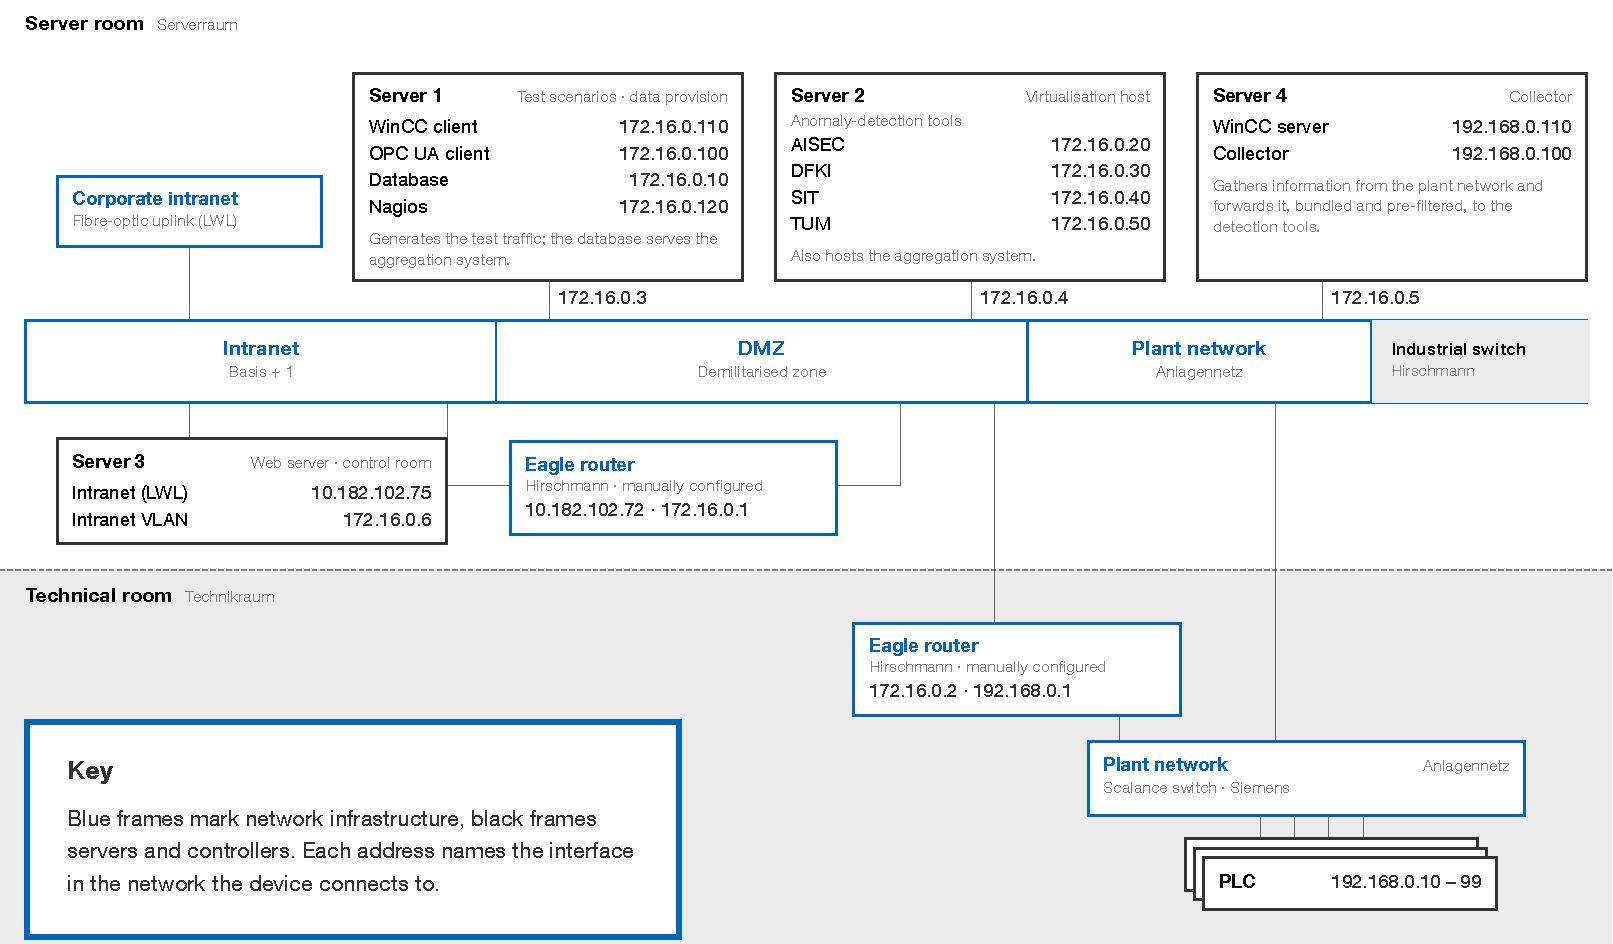
\includegraphics[width=\textheight]{iuno-VW_testbed.pdf}
  \caption{The IUNO test environment at the Volkswagen plant in Wolfsburg. Four servers, three
  network segments and a Siemens plant network reproduce the production setting in which
  \nadics{} ran as the TUM detection tool on the virtualisation host. The network TAPs fitted at
  the relevant interfaces are omitted from the drawing \cite{iuno2017d42}.}
  \label{fig:anomaly:iuno-testbed}
\end{sidewaysfigure}

Figure~\ref{fig:anomaly:iuno-testbed} shows where the framework ran. The environment was built
at the Volkswagen plant in Wolfsburg from hardware of the kind used in regular production
\cite{iuno2017d42}. A Hirschmann industrial switch carries three segments, the intranet, the
demilitarised zone and the plant network, and manually configured Eagle routers separate them.
The first of four servers runs the WinCC and OPC~UA clients that originate test traffic, together
with a Nagios instance and the database of the aggregation system. The second is the
virtualisation host for the detection tools contributed by AISEC, DFKI, SIT and TUM, and the
third serves the visual control room to the intranet. The fourth combines the WinCC server with
the collector, which gathers traffic from the plant network and passes it, bundled and
pre-filtered, to the detection tools, so \nadics{} was one of four detectors reading the same
collector output. Siemens controllers occupy the plant network behind a Scalance switch. The
collector observed that network passively at the plant switch, never in line with the traffic,
which matches the detection-only design: an alert could reach the control room, but nothing in
the path could stop a packet.

The IUNO deliverables describe the tool and its environment but print no measured result for it
\cite{iuno_ap4}. The values below come from the experimental records of the project and cover
the corpus and its feature schema, the detection results on the held-out session, the alarm
burden over a benign monitoring period, and the throughput of the extractor on the prototype
collector.

\subsection{The S7-300 Corpus}
\label{sec:anomaly:iuno-corpus}

The corpus was recorded in 2018 in the environment of Figure~\ref{fig:anomaly:iuno-testbed},
where six Siemens S7-300 controllers exchanged routine polling and control traffic with
WinCC-based services. Complete selected channels were kept, together with ARP and DCP traffic and
the connection attempts belonging to those channels. No random packet sampling was applied.

Recording opened with a two-hour clean baseline, which was excluded from the corpus totals. That
interval fixed the communication relationships, the polling behaviour and the protocol activity
expected under the operating modes present at the time. Six capture sessions followed, with 24
hours of labelled traffic in total. The collector recorded 12,616,875 Ethernet frames in that
period, an average of 146.03 frames per second. The captured frames hold 2,317,074,962 bytes,
and the six capture files occupy about 2.519~GB in the classic PCAP format.

Twenty-five controlled attack episodes were executed during the sessions, five repetitions of
each of the five classes the deliverable names \cite{iuno_ap4}. Background communication
continued while they ran. Table~\ref{tab:anomaly:iuno-episodes} lists the duration of every
episode. The shortest lasted 3~min 07~s and the longest 9~min 55~s, and together they cover
2~h 51~min 05~s. Episodes also differed in the channels they touched and in how often a
connection was re-established. Labels were assigned
from the execution logs and from inspection of the packet traces, and only the communications an
episode actually affected received an attack label, so background traffic concurrent with an
attack keeps the normal label. Two attack types were never run against one channel at the same
time.

\begin{table}[tbp]
  \centering
  \caption{Composition of the S7-300 corpus and its partitions. Whole capture sessions were
  assigned to the partitions, four to training and one to each of the other two, and every
  attack episode lies entirely within one partition. The episode column counts executed attacks,
  not records.}
  \label{tab:anomaly:iuno-corpus}
  \small
  \begin{tabular}{@{}lrrrrr@{}}
    \toprule
    Class & Corpus & Train & Validation & Test & Episodes \\
    \midrule
    Normal                 & 113,751 & 76,556 & 18,587 & 18,608 &    \\
    Authentication bypass  &   1,058 &    441 &    269 &    348 &  5 \\
    CPU stop and start     &     593 &    359 &     90 &    144 &  5 \\
    Reconnaissance         &   1,803 &  1,070 &    366 &    367 &  5 \\
    Denial of service      &   1,230 &    765 &    278 &    187 &  5 \\
    Brute force            &     725 &    445 &     93 &    187 &  5 \\
    \midrule
    Total                  & 119,160 & 79,636 & 19,683 & 19,841 & 25 \\
    Capture time (h:min:s) & 24:00:00 & 16:01:57 & 3:56:27 & 4:01:36 & \\
    \bottomrule
  \end{tabular}
\end{table}

\begin{table}[tbp]
  \centering
  \caption{Duration of the 25 attack episodes in minutes and seconds. Each attack type has three
  training episodes, one validation episode and one test episode.}
  \label{tab:anomaly:iuno-episodes}
  \small
  \begin{tabular}{@{}llrrr@{}}
    \toprule
    Class & Training episodes & Validation & Test & All five \\
    \midrule
    Authentication bypass & 5:33, 4:01, 5:50 & 7:16 & 9:34 & 32:14 \\
    CPU stop and start    & 7:03, 8:23, 3:07 & 4:04 & 7:39 & 30:16 \\
    Reconnaissance        & 6:42, 9:40, 7:28 & 9:55 & 8:27 & 42:12 \\
    Denial of service     & 6:41, 9:39, 7:07 & 7:46 & 5:38 & 36:51 \\
    Brute force           & 8:05, 3:16, 4:06 & 4:15 & 9:50 & 29:32 \\
    \midrule
    Total                 &                  &      &      & 171:05 \\
    \bottomrule
  \end{tabular}
\end{table}

Extraction produced 119,160 feature records. Of these, 113,751 are normal and 5,409 carry one of
the five attack labels, an attack share of 4.54 per cent. Table~\ref{tab:anomaly:iuno-corpus}
gives the composition. The training sessions hold 79,636 records, the validation session 19,683
and the test session 19,841. Each attack type contributes three training episodes and one
episode to each of the remaining partitions, and because episodes differ in duration and in the
channels they touch, the attack records of a class are not divided between the partitions in a
fixed proportion. An episode, its recovery interval and the windows that depend on it stay inside
a single partition, and no rolling window crosses a partition boundary. The attack counts must
not be read as a count of attacks. A single episode of a few minutes generates many records,
and the corpus averages about 216 affected records per episode.

The extraction schema has 63 fields in five groups: 18 flow fields, 13 timing fields, 18
protocol fields, nine relational fields and five process fields. Forty-six are numerical, eleven
categorical and six binary, and encoding of the categorical fields expands the input
dimensionality of the model. The flow group follows the output of Argus and Bro-IDS, which the
extractor wrapped. Protocol fields cover S7 message and function codes,
addressed memory areas, address entropy and error codes, together with COTP and OPC~UA fields.
Relational fields describe the communication partners, the age of an edge, and the number of
distinct destinations and ports observed in the preceding minute. The process group reads one
preconfigured anchor tag per channel, whose identity and units are held as metadata, so a value
delta is never computed across unrelated tags. Unobservable protocol fields carry an explicit
missing state, and an absent OPC~UA security policy is not encoded as the policy \emph{None}.

\begin{figure}[tbp]
  \centering
  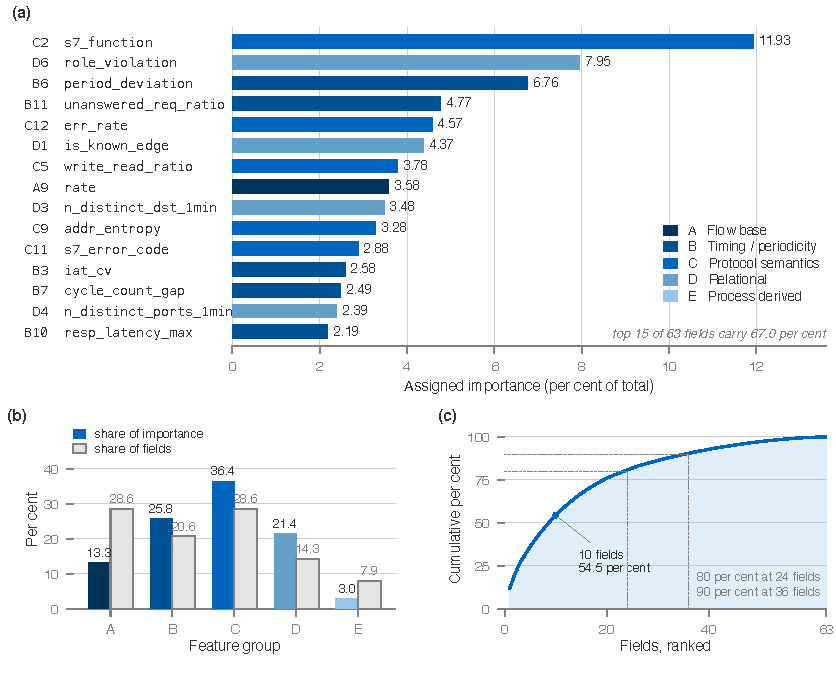
\includegraphics[width=\linewidth]{nadics-feature-importance.pdf}
  \caption{Random-forest importance of the 63 extraction fields. (a) The fifteen most
  important fields, coloured by group. (b) Each group's share of the total importance
  against its share of the field count. (c) Cumulative share over the ranked fields.}
  \label{fig:anomaly:iuno-importance}
\end{figure}

Figure~\ref{fig:anomaly:iuno-importance} shows the importance of each field in the random forest
of Section~\ref{sec:anomaly:iuno-results}. The forest was fitted to the training partition; the
impurity reductions from splits on each field were summed across its trees, normalised over all
63 fields, and ranked. Panel~(a) shows the fifteen highest, and
Appendix~\ref{app:nadics-importance} lists all 63. \texttt{s7\_function} leads at 11.9 per cent,
because a stop or a start is an ordinary S7 operation whose function code is visible in the
request, and \texttt{role\_violation} follows at 8.0 per cent, because a write from a host whose
role does not write is anomalous even over an established connection. Both signals have limits:
legitimate maintenance issues the same function codes, and a compromised engineering station
writes from a role that is permitted to write.

Panel~(b) sets each group's share of the total importance against its share of the fields.
Protocol semantics holds the largest share at 36.4 per cent, although it also holds the most
fields. The comparison that carries information is the share per field: the nine relational
fields average 2.38 per cent each, against 0.74 for the eighteen flow fields and 0.60 for the five
process fields. Only the process fields receive less importance per field than the flow
statistics. That is consistent with the position the schema takes: an
industrial detector built on Argus and Bro flow features alone discards most of what separates an
S7 attack from S7 polling. Panel~(c) gives the cumulative share. Ten fields reach 54.5 per cent
of the total importance, twenty-four reach 80 per cent and thirty-six reach 90 per cent, so the
tail of the schema is thin and a reduced schema is plausible. \nadics{} exposes an importance
ranking for exactly this purpose \cite{iuno_ap4}.

One record covers a non-overlapping ten-second window of an activity-bearing connection or
channel, and a shorter final record is written when a session closes. PROFINET RT traffic is
keyed at layer 2, since it carries no transport-layer connection. The windowing refines the
per-connection unit of Figure~\ref{fig:anomaly:nadics-arch} so that a change during a long-lived
session can be scored while the session is still open. Channels that fall silent emit no record.

Three definitions were adjusted so that no record depends on information from after its own
window closes. The duration field measures the exported segment and not the eventual lifetime of
an open connection, while a separate field retains the time elapsed since the underlying
connection opened. The ratio of unanswered requests counts only those requests whose one-second
response deadline had already expired at window closure, and pending requests are excluded from
both the numerator and the denominator. Trailing source and timing state is held over 60
seconds, and the period features are computed from past observations. Encoders, imputation and
scaling were fitted on the training partition alone, and the classifier together with its
preprocessing was then held fixed for validation and testing.

\subsection{Detection Results}
\label{sec:anomaly:iuno-results}

The classifier is a random forest of 300 trees with a maximum depth of 16 and a minimum leaf
size of five. Class weighting was applied per bootstrap sample, and the training data were not
resampled. Two decisions were read from the same fitted model: a binary verdict of normal
against attack, and an assignment to one of six classes, the normal class and the five attack
types. Every figure below comes from the held-out test session, which holds 18,608 normal and
1,233 attack records.

\begin{table}[tbp]
  \centering
  \caption{Six-class confusion matrix on the 19,841-record test session, with rows giving the
  true class. Predicted classes are abbreviated: N normal, AB authentication bypass, CS CPU stop
  and start, RC reconnaissance, DS denial of service, BF brute force. The last three columns
  give precision, recall and $F_1$ for the class of that row.}
  \label{tab:anomaly:iuno-confusion}
  \small
  \setlength{\tabcolsep}{4.5pt}
  \begin{tabular}{@{}lrrrrrrrrr@{}}
    \toprule
    & \multicolumn{6}{c}{Predicted class} & \multicolumn{3}{c}{Score (\%)} \\
    \cmidrule(lr){2-7}\cmidrule(l){8-10}
    True class & N & AB & CS & RC & DS & BF & Prec. & Rec. & $F_1$ \\
    \midrule
    Normal                & 18,518 &  21 &   5 &  31 &  18 &  15 & 99.74 & 99.52 & 99.63 \\
    Authentication bypass &     22 & 292 &   8 &  12 &   1 &  13 & 88.75 & 83.91 & 86.26 \\
    CPU stop and start    &      3 &   1 & 134 &   2 &   3 &   1 & 90.54 & 93.06 & 91.78 \\
    Reconnaissance        &      9 &   7 &   0 & 337 &   6 &   8 & 84.25 & 91.83 & 87.87 \\
    Denial of service     &      5 &   0 &   0 &   4 & 178 &   0 & 85.99 & 95.19 & 90.36 \\
    Brute force           &      9 &   8 &   1 &  14 &   1 & 154 & 80.63 & 82.35 & 81.48 \\
    \bottomrule
  \end{tabular}
\end{table}

Table~\ref{tab:anomaly:iuno-confusion} reports the six-class confusion matrix together with the
per-class scores. Collapsing the same predictions into the binary decision gives 18,518 true
negatives, 90 false positives, 48 false negatives and 1,185 true positives. Binary accuracy is
99.30 per cent, attack precision 92.94 per cent and attack recall 96.11 per cent, for an attack
$F_1$ of 94.50 per cent. The false-positive rate over normal records is 0.484 per cent and the
balanced accuracy 97.81 per cent. On the six-class task, accuracy reaches 98.85 per cent, the
macro-$F_1$ 89.56 per cent and the weighted $F_1$ 98.86 per cent.

Accuracy is the least informative of these numbers. Normal records make up 93.79 per cent of the
test partition, so a detector that never fired would already score 93.79 per cent, and the gap
between the weighted and the macro $F_1$, 98.86 against 89.56 per cent, measures how much of the
six-class figure the normal class carries. Per-class recall is highest for denial of service at
95.19 per cent and lowest for brute force at 82.35 per cent, with authentication bypass close
behind at 83.91 per cent. Most errors of these two classes fall on other attack classes.
Authentication bypass loses 22 of its 348 records to the normal class and 34 to the other attack
types, while brute force loses nine of its 187 records to the normal class and 24 to the other
attack types, 14 of them to reconnaissance. Both attacks reuse the protocol operations of
legitimate engineering access, so a window holding only a few such operations offers little that
separates them from ordinary traffic or from each other.

All of these scores are computed over records. They show that the extracted features separate
the five executed attacks from the surrounding traffic of this plant under a session-disjoint
split.

\subsection{Benign Operation and Alarm Burden}
\label{sec:anomaly:iuno-field}

A second exercise measured what the detector does when nothing malicious happens. It ran in the
Volkswagen environment with four active PLCs and ordinary supervisory traffic. A separate
two-hour baseline preceded 24 hours of benign monitoring. Over that day the collector recorded
8,472,913 frames, an average of 98.07 frames per second. The captured frames hold 2,186,039,471
bytes, about 2.322~GB in the classic PCAP format, and the extractor emitted 83,847 records.
Engineering work and planned device restarts took place during the period and count as benign.

The detector classified 83,740 records as normal and 107 as attacks, all of them false, a
record-level false-positive rate of 0.128 per cent. Positives were merged into alarm episodes
before presentation to the control room: positives that share a source, a destination and a
predicted attack class belong to one episode, and an episode closes once 60 seconds pass without
a further positive. One notification opens an episode, and later positives update it. Nine alarm
episodes were raised over the day, 0.375 per hour on average, and each was assigned a benign
cause. Engineering workstation activity accounts for 43 positive records in three episodes and
OPC~UA reconnections for 28 records in two. Brief communication interruptions produced 23
records in two episodes, and planned device restarts 13 records in two.

No attack was executed during this period, so every alarm it raised was false. Its 0.128 per
cent record rate lies below the 0.484 per cent of the test session, whose normal records also
include the recovery intervals of executed attacks. The recovered causes share a structure that
matters for deployment: each is a legitimate departure from routine polling, so the alarm burden
of this design follows the rate at which such events occur in the plant.

\subsection{Extractor Throughput on Constrained Hardware}
\label{sec:anomaly:iuno-pi}

The extractor was also exercised on a Raspberry Pi 3 Model B. The deliverable of June 2017
names Raspberry Pi boards as the prototype platform \cite{iuno2017d42}. The board carries four
cores at 1.2~GHz, 1~GB of RAM and 100~Mbit/s Ethernet. Only the extraction stage ran on it,
comprising selected-field capture and dissection of S7comm and PROFINET traffic, the bounded rolling
feature computations and emission of CSV or JSON. Model fitting and inference remained on the
server, and archival of full packet captures to the SD card was excluded. Each load replayed
traffic over 100 configured communication channels with varying channel activity for about ten
minutes.

\begin{table}[tbp]
  \centering
  \caption{Extraction workloads on the Raspberry Pi 3 prototype. Input frames are the frames
  presented to the extraction pipeline, and processed frames exclude those dropped before
  processing. Rates and CPU utilisation are averages over the replay, and CPU utilisation refers
  to the capacity of the whole device.}
  \label{tab:anomaly:iuno-pi}
  \small
  \begin{tabular}{@{}lrrr@{}}
    \toprule
    Quantity & Light load & Moderate load & Overload \\
    \midrule
    Replay duration (s)                 &  600.14 &    599.87 &    600.09 \\
    Input frames                        & 599,827 & 1,498,463 & 2,100,731 \\
    Dropped frames                      &       4 &       361 &   245,897 \\
    Processed frames                    & 599,823 & 1,498,102 & 1,854,834 \\
    Frame loss (\%)                     & 0.00067 &   0.02409 &  11.70531 \\
    Input rate (frames/s)               &  999.48 &  2,497.98 &  3,500.69 \\
    Processed rate (frames/s)           &  999.47 &  2,497.38 &  3,090.93 \\
    Feature records                     &   5,842 &     5,887 &     5,781 \\
    \midrule
    Mean CPU utilisation (\%)           &    22.6 &      43.1 &      50.4 \\
    Peak extractor memory (MiB)         &     302 &       381 &       436 \\
    95th-percentile emission delay (ms) &      96 &       234 &       817 \\
    \bottomrule
  \end{tabular}
\end{table}

Table~\ref{tab:anomaly:iuno-pi} reports the three loads. At the moderate load, 1,498,463 frames
were presented in 599.87 seconds and 361 were dropped, a loss of 0.024 per cent at a processed
rate of 2,497.38 frames per second. This input rate is about 17 times the average frame rate of
the corpus capture. The extractor used 43.1 per cent of the CPU capacity of the device on average
and at most 381~MiB of memory. The 95th percentile of the delay from the close of a window to the
emission of its record was 234~ms, a delay that excludes the ten seconds in which the window
accumulates. The light load lost four of its 599,827 frames at 22.6 per cent CPU utilisation.
The overload row does not describe a supported rate: 11.71 per cent of the input was dropped,
and the processed rate stayed at 3,090.93 frames per second against an input rate of 3,500.69.
Mean CPU utilisation reached 50.4 per cent there, and the 95th-percentile emission delay rose to
817~ms. The three runs emitted 5,842, 5,887 and 5,781 records, fewer than the 6,000 that 100
continuously active channels would give in ten-second windows over ten minutes, because channel
activity varied.

\section{A GAN-Based Multivariate Detector for SWaT}
\label{sec:anomaly:gan}

Industrial process recordings form multivariate time series: each timestamp associates sensor
measurements with actuator states, and successive observations describe the evolution of the
plant. An anomaly may appear as an unusual value or as a sequence that conflicts with the
expected relationships between variables. A measurement within its usual range can therefore
be anomalous in its temporal or process context. MAD-GAN motivates joint modelling of these
dependencies for industrial intrusion detection, while TadGAN addresses anomalous sequences
across several time-series domains \cite{li2019madgan,geiger2020tadgan}. Process monitoring can
expose the physical effects of an attack, although a deviation alone does not establish its
cause. Scarce labelled attack examples motivate methods that learn reference behaviour from
recorded operation.

A generative adversarial network (GAN) learns a data distribution through two neural networks
with opposing training objectives \cite{goodfellow2014generative}. The generator transforms
samples from a latent distribution into synthetic observations. The discriminator learns to
distinguish recorded observations from generated samples, and the generator is updated to make
that distinction harder. For time series, the generated objects are sequences of measurements.
Here, \emph{adversarial} describes the training relationship between the networks. The
discriminator's training labels identify recorded and generated data; they are not attack
annotations.

For anomaly detection, the learned distribution provides a reference against which new
observations can be assessed. MAD-GAN uses long short-term memory (LSTM) networks to model
multivariate windows and combines discrimination with reconstruction error
\cite{li2019madgan}. Reconstruction requires a latent representation from which the generator
can reproduce the observed sequence; MAD-GAN searches for this representation at inference.
TadGAN learns an encoder for this mapping and adds a cycle-consistency loss that penalises
differences between an input and its reconstruction. Its Wasserstein critics supply real-valued
scores for matching distributions during training \cite{geiger2020tadgan}. Reconstruction error
and discriminator or critic output can then supply evidence of deviation. Their usefulness
depends on the behaviour represented in training and on the subsequent scoring rule.

The present study combines multivariate process windows with the encoder and cycle-consistent
training of TadGAN. It examines how five input representations affect detection and false alarms
on a fixed SWaT evaluation cohort. The experiment concerns a detector developed with some
attack observations, as specified below; its learned reference therefore includes both normal
and attack behaviour. This distinction matters when comparing its results with methods trained
only on normal operation.

The detector operates on process measurements from the Secure Water Treatment (SWaT) testbed.
SWaT comprises six treatment stages, with programmable logic controllers coordinating sensors
and actuators and a supervisory network connecting the controllers to supervisory control and data acquisition (SCADA)
(Figure~\ref{fig:anomaly:swat-architecture}). The process dataset contains 51 sensor and
actuator variables recorded at a nominal frequency of one observation per second
\cite{goh2016swatdataset}. These variables describe the physical behaviour of the plant,
allowing the detector to consider changes in individual measurements together with relationships
among measurements across the treatment process.

\begin{figure}[htbp]
  \centering
  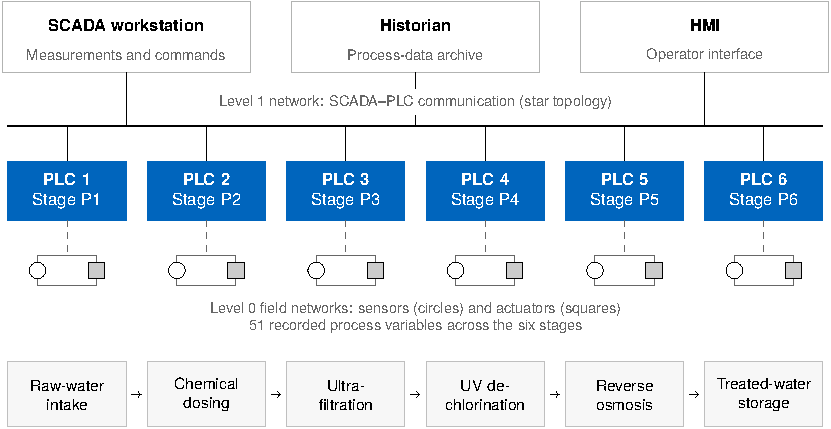
\includegraphics[width=\linewidth]{swat/thesis/swat-ics-architecture.pdf}
  \caption{SWaT process and control architecture. Network levels follow the SWaT convention.
  The field-network symbols indicate sensors and actuators within each stage; the detector
  consumes their recorded values. Adapted from the supplied diagram and the dataset
  description \cite{goh2016swatdataset}.}
  \label{fig:anomaly:swat-architecture}
\end{figure}

The dataset documentation describes 36 attacks distributed across four categories
(Figure~\ref{fig:anomaly:swat-taxonomy}): 26 single-stage, single-point attacks; four
single-stage, multiple-point attacks; two multiple-stage, single-point attacks; and four
multiple-stage, multiple-point attacks \cite{goh2016swatdataset}. These categories describe the
scope of the interventions. They do not imply that all attacks produce equally observable process
changes. An intervention affecting one sensor or actuator may also influence measurements
elsewhere in the plant, while an attack with little physical effect may remain difficult to
identify from process data alone. The aggregate calculations in this section concern anomalous
timestamps and do not establish the number of individual attacks detected.

\begin{figure}[htbp]
  \centering
  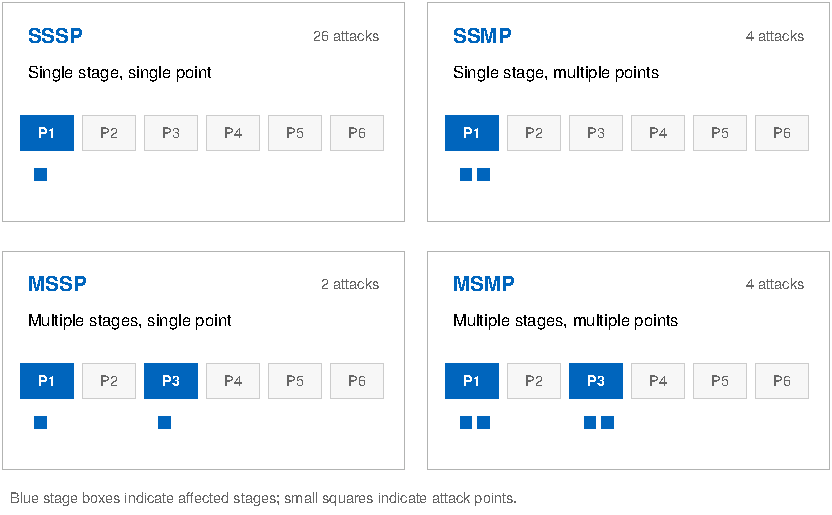
\includegraphics[width=\linewidth]{swat/thesis/swat-attack-taxonomy.pdf}
  \caption{SWaT attack categories and their counts in the dataset paper
  \cite{goh2016swatdataset}. Stage and point locations are schematic examples. The
  arrangement describes attack scope and carries no ranking of detection difficulty.}
  \label{fig:anomaly:swat-taxonomy}
\end{figure}

The source collection campaign comprises seven days of normal operation followed by four days
containing attacks \cite{goh2016swatdataset}. Preprocessing removes the first 21,600 observations
from the normal-operation trace, which cover the initial six-hour stabilisation period
(Figure~\ref{fig:anomaly:swat-campaign}). The empirical study uses all 449,919 timestamps of the
attack-period recording. Its first 56,240 timestamps are divided between the training and
validation partitions, which also receive separate portions of the normal-operation recording.
The later 393,679 attack-period timestamps form the test set. They comprise 51,453 anomalous and
342,226 normal timestamps, so anomalous observations account for 13.07\% of the test cohort.

\begin{figure}[htbp]
  \centering
  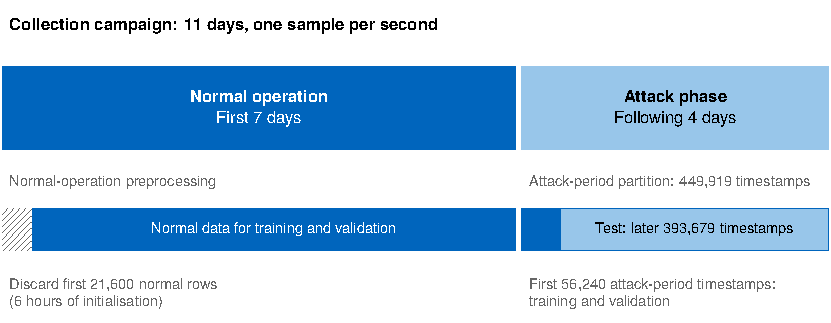
\includegraphics[width=\linewidth]{swat/thesis/swat-collection-campaign.pdf}
  \caption{SWaT collection campaign and the partition used in the GAN study. The campaign
  follows the dataset paper \cite{goh2016swatdataset}. After the initial normal-operation
  exclusion, the first 56,240 attack-period timestamps support training and validation; the
  later 393,679 timestamps form the test set.}
  \label{fig:anomaly:swat-campaign}
\end{figure}

All three partitions contain normal observations and labelled attack examples. Each attack
episode is confined to one partition, and no window crosses a partition boundary or a
discontinuity in the recordings. Partitioning precedes imputation, scaling, feature selection
and window construction. Earlier observations support model development, while the later
observations form the test cohort.

The GAN objective does not require class annotations during gradient-based fitting.
Nevertheless, the complete procedure includes supervised feature selection and model
selection, and training includes attack observations. The resulting evaluation therefore
concerns a detector developed with prior exposure to attacks. It does not establish detection
performance for previously unseen attack types or a wholly unsupervised development process.

\subsection{Model and Training}
\label{sec:anomaly:gan-method}

The model contains four jointly trained networks: an encoder, a generator, a data critic and a
latent critic (Figure~\ref{fig:anomaly:gan-pipeline}). For an input window $X$, the encoder $E$
maps the observed process sequence to a latent representation $E(X)$. The generator $G$ maps
this representation back to the observation space, producing the reconstruction
\[
  \widehat{X}=G(E(X)).
\]
Latent samples $z$ are drawn from a standard normal distribution. The data critic compares
observed windows with generated windows $G(z)$, encouraging the generator to reproduce the
distribution of the training sequences. The latent critic compares encoded observations $E(X)$
with samples from the latent prior. A cycle-consistency term penalises discrepancies between an
observed window and its reconstruction,
\[
  \mathcal{L}_{\mathrm{cyc}}
  =\mathbb{E}_{X}\!\left[\left\lVert X-G(E(X))\right\rVert_2\right].
\]

\begin{figure}[tbp]
  \centering
  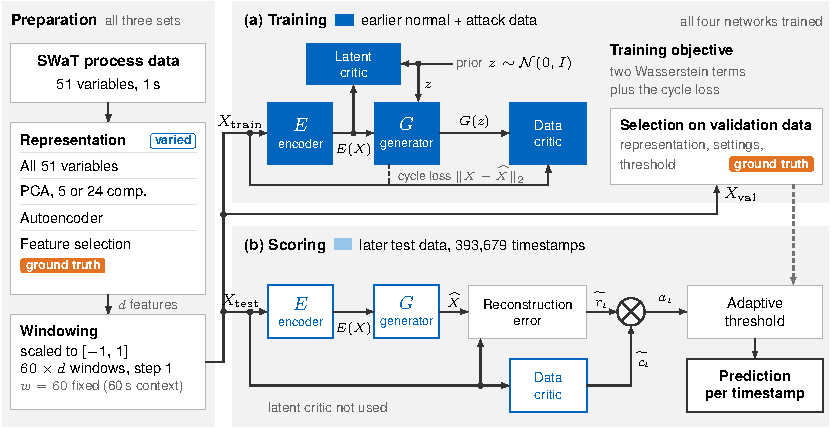
\includegraphics[width=\linewidth]{swat/thesis/swat-gan-pipeline.pdf}
  \caption{Multivariate GAN detection pipeline. (a) The four networks are trained together on
  earlier windows containing normal and attack observations. (b) The later 393,679 test timestamps are
  scored with the trained networks; the latent critic has no part in the score $a_t$ of
  Equation~\ref{eq:anomaly:gan-score}. The blue tag marks the input representation, the only
  factor varied between runs, and orange tags mark development steps that used attack ground truth. The
  window length is fixed at 60 samples.}
  \label{fig:anomaly:gan-pipeline}
\end{figure}

Training combines the two Wasserstein objectives with this reconstruction constraint. The
encoder provides a direct mapping from process observations to latent representations, while
the cycle-consistency term encourages those representations to retain information required to
reconstruct the input. The data critic supplies an additional measure of how closely an observed
sequence resembles the learned training distribution. The latent critic contributes to training
and is not included in the anomaly score at inference \cite{geiger2020tadgan}.

At inference, each test window is encoded and reconstructed using the fitted model.
Discrepancies between the observed and reconstructed sequences provide a reconstruction score
(Figure~\ref{fig:anomaly:gan-reconstruction}). The data critic supplies a second score for the
observed window. Before combination, the scores require a common orientation, such that larger
values indicate greater deviation from the reference behaviour. Their normalisation must also
prevent a product of two negative standardised values from being interpreted as strong anomalous
evidence. The reported score therefore uses non-negative, consistently oriented normalised
components:
\begin{equation}
  a_t=\widetilde{r}_t\,\widetilde{c}_t.
  \label{eq:anomaly:gan-score}
\end{equation}

\begin{figure}[htbp]
  \centering
  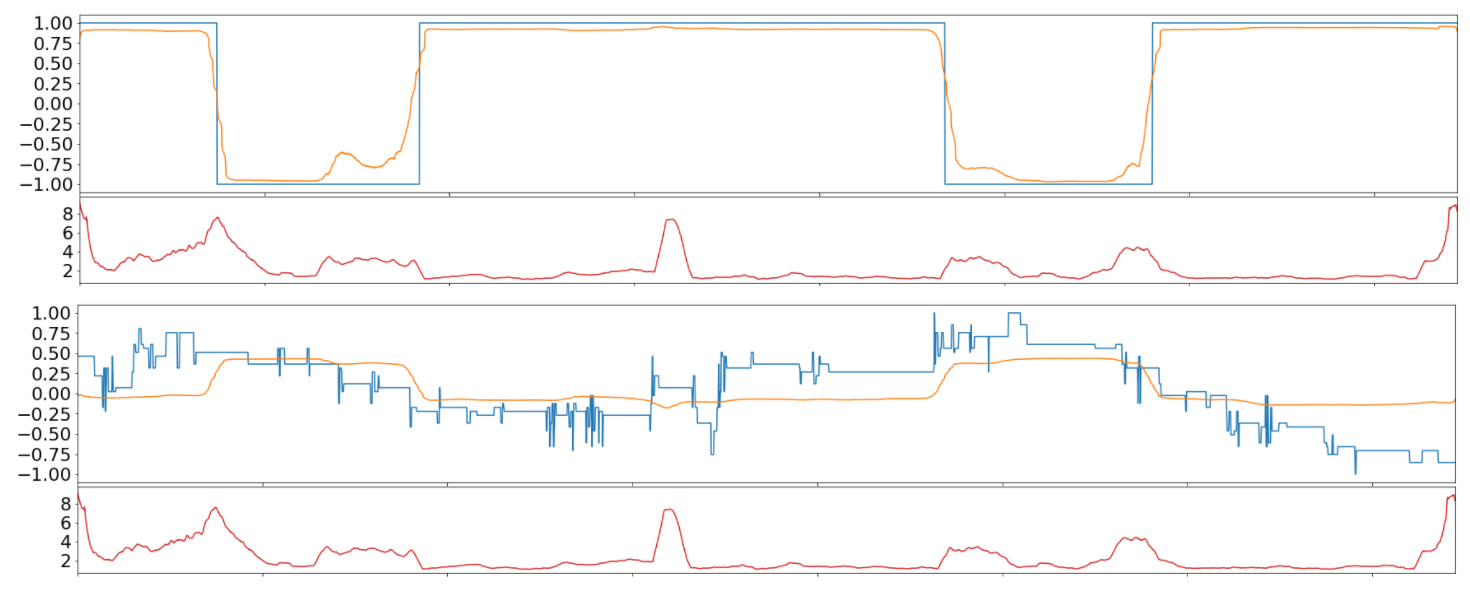
\includegraphics[width=\linewidth]{swat/report-originals/report-fig-4.15-reconstruction.png}
  \caption{Observed signals (blue) and their reconstructions (orange) for two dimensions. The
  repeated red trace is the aggregate reconstruction discrepancy across dimensions, shared by
  the two displayed signals. It precedes the combination of
  Equation~\ref{eq:anomaly:gan-score}.}
  \label{fig:anomaly:gan-reconstruction}
\end{figure}

Score transformations are fitted on development data and fixed during evaluation. Reconstruction
discrepancy and critic output jointly indicate deviation, without providing a calibrated attack
probability. Normal operational changes can also produce high reconstruction error.

For each timestamp, overlapping-window reconstructions are averaged per variable before
calculating the multivariate reconstruction discrepancy; critic outputs are averaged separately.
Only windows within the same partition contribute. Each timestamp receives one combined score
and prediction and is counted once in the confusion matrix.

An adaptive threshold converts scores into binary predictions and may merge adjacent anomalous
intervals. Its historical context is distinct from the networks' 60-second input window.
Because aggregation includes observations later than the timestamp being scored, the results
describe offline detection; online performance and real-time detection delay remain unevaluated.

\subsection{Input Representations and Settings}
\label{sec:anomaly:gan-inputs}

The representation comparison includes the complete set of 51 process variables, two principal
component analysis (PCA) configurations, an autoencoder representation and a selected feature
subset. The full representation retains the original measurements and actuator states. It
provides the broadest input coverage but also exposes the model to redundant relationships and
normal operational variation across the process.

PCA projects the measurements onto $k$ orthogonal components. Let
$\lambda_1\geq\cdots\geq\lambda_{51}\geq0$ denote the eigenvalues of the covariance matrix
estimated from training data. The retained variance fraction is
\[
  \rho_k=\frac{\sum_{j=1}^{k}\lambda_j}{\sum_{j=1}^{51}\lambda_j}.
\]
The study compares $k=5$ and $k=24$, with $\rho_{24}\approx0.99$. Retained variance does not
quantify attack-relevant information; low-variance directions may still distinguish attacks.

The autoencoder learns a nonlinear representation for reconstruction before GAN processing.
Feature selection combines correlation analysis with chi-squared selection, recursive feature
elimination, LASSO and Random Forest importance. Supervised selectors use training labels only.
Any non-negative transformation required for chi-squared selection is fitted separately from GAN scaling.
The aggregate results do not specify the selected variables or the autoencoder bottleneck dimension.

All preprocessing is fitted on training data and reused for validation and testing. GAN inputs
use a training-derived scale with reference range $[-1,1]$. Values outside the training range
remain unclipped to preserve deviations.

For feature vectors $\mathbf{y}_t\in\mathbb{R}^{d}$, each window is
\[
  X_t=[\mathbf{y}_t,\ldots,\mathbf{y}_{t+59}]^{\mathsf T}
  \in\mathbb{R}^{60\times d}.
\]
At the nominal sampling rate, this gives a 60-second context with a one-second stride.
An uninterrupted sequence of $N\geq60$ observations yields
$N-60+1$ windows; performance metrics count timestamps after aggregation.

The final configuration uses Adam with learning rate $5\times10^{-4}$, latent dimension 20,
batch size 64 and 50 epochs. All variants share the evaluation cohort and counting convention.
Attribution of performance differences to the input representation requires control of network
capacity and tuning effort.

The reference computing platform comprises an AMD EPYC 7551P processor with 32 cores, 125\,GB of
RAM and a TITAN X GPU with 12\,GB of memory. These specifications describe the reported execution
environment. They do not establish training duration, inference throughput or memory
consumption. Reducing the input dimension from 51 variables to 24 components constitutes a
52.94\% reduction in input dimensionality; computational savings would require direct
measurement.

\subsection{Detection Results}
\label{sec:anomaly:gan-results}

Table~\ref{tab:anomaly:gan-representations} presents the measured performance of
the five input configurations. Each row uses the same class totals: 51,453 anomalous timestamps
and 342,226 normal timestamps. Precision describes the proportion of predicted anomalous
timestamps that fall within recorded attack periods. Recall describes the proportion of actual
anomalous timestamps that are detected. $F_1$ is the harmonic mean of precision and recall, while the
false-positive rate is the proportion of normal timestamps incorrectly flagged. All table entries
are calculated from integer confusion counts and rounded to two decimal places.

\begin{table}[tbp]
  \centering
  \caption{Measured timestamp-level performance of the input representations. Each timestamp
  is counted once and no point adjustment is applied.}
  \label{tab:anomaly:gan-representations}
  \small
  \begin{tabular}{@{}lrrrr@{}}
    \toprule
    Input representation & Precision (\%) & Recall (\%) & $F_1$ (\%) & False-positive rate (\%) \\
    \midrule
    All 51 variables           & 70.00 & 94.50 & 80.43 & 6.09 \\
    PCA: 5 components          & 75.00 & 86.50 & 80.34 & 4.34 \\
    PCA: 24 components         & 73.00 & 92.00 & 81.41 & 5.12 \\
    Autoencoder representation & 72.00 & 86.50 & 78.59 & 5.06 \\
    Selected feature subset    & 71.00 & 84.00 & 76.96 & 5.16 \\
    \bottomrule
  \end{tabular}
\end{table}

The complete representation has the highest recall, at 94.50\%, together with the
highest false-positive rate, at 6.09\%. This profile represents a detector that identifies a
larger proportion of anomalous observations while also flagging more normal observations. The
five-component PCA configuration has the highest precision, at 75.00\%, and the lowest
false-positive rate, at 4.34\%, accompanied by lower recall of 86.50\%. In these results,
stronger compression therefore corresponds to fewer false-positive timestamps and more
missed anomalous timestamps.

The 24-component PCA configuration provides an intermediate balance, with precision of 73.00\%,
recall of 92.00\% and an $F_1$ score of 81.41\%. Relative to the complete representation, its
precision is 3.00 percentage points higher and its recall is 2.50 percentage points lower. Its
$F_1$ score is approximately 0.98 percentage points higher. This configuration has the highest
reported $F_1$ and is used for the detailed analysis below. The numerical difference does not
establish a statistically reliable advantage or a preference under every operational cost model.

The autoencoder representation has a precision of 72.00\% and recall of 86.50\%,
corresponding to an $F_1$ score of 78.59\%. The selected feature subset has precision of
71.00\%, recall of 84.00\% and $F_1$ of 76.96\%. These values show lower detection coverage
for the two configurations. They do not identify a causal mechanism: loss of
relevant input information, differences in representation learning and changes in model
capacity would require separate investigation.

The final 24-component PCA evaluation produced the confusion matrix in
Table~\ref{tab:anomaly:gan-confusion}: 47,337 of the 51,453 anomalous timestamps are detected
and 17,508 of the 342,226 normal timestamps are flagged as anomalous.

\begin{table}[tbp]
  \centering
  \caption{Timestamp-level confusion matrix for the final 24-component PCA configuration. Counts
  refer to individual timestamps after aggregation of overlapping window outputs.}
  \label{tab:anomaly:gan-confusion}
  \small
  \begin{tabular}{@{}lrrr@{}}
    \toprule
    Actual class & Predicted anomalous & Predicted normal & Total \\
    \midrule
    Anomalous & 47,337 (TP) &   4,116 (FN) &  51,453 \\
    Normal    & 17,508 (FP) & 324,718 (TN) & 342,226 \\
    \midrule
    Total     & 64,845      & 328,834      & \textbf{393,679} \\
    \bottomrule
  \end{tabular}
\end{table}

The performance measures follow directly from these counts and are calculated from the
unrounded values:
\begin{alignat*}{3}
  \mathrm{Precision} &= TP/(TP+FP)          &&= 47{,}337/64{,}845   &&= 73.00\%,\\
  \mathrm{Recall}    &= TP/(TP+FN)          &&= 47{,}337/51{,}453   &&= 92.00\%,\\
  F_1                &= 2TP/(2TP+FP+FN)     &&= 94{,}674/116{,}298  &&= 81.41\%,\\
  \mathrm{FPR}       &= FP/(FP+TN)          &&= 17{,}508/342{,}226  &&= 5.12\%,\\
  \mathrm{Accuracy}  &= (TP+TN)/(TP+FN+FP+TN) &&= 372{,}055/393{,}679 &&= 94.51\%.
\end{alignat*}

The recall of 92.00\% means that the detector flags approximately 92 of every 100 anomalous
timestamps. It does not mean that 92\% of attack episodes are detected. Long attacks contribute
more timestamps than short attacks, so the same timestamp-level recall could arise from
different distributions of detection across attack episodes. Precision of 73.00\% means that
approximately 27\% of flagged timestamps fall within recorded normal periods. This proportion
differs from the false-positive rate of 5.12\%, whose denominator includes all normal
timestamps.

Accuracy is interpreted alongside the class distribution. Since normal observations account for
86.93\% of the cohort, a rule assigning every observation to the normal class would achieve
86.93\% accuracy while detecting no anomalous timestamps. The measured accuracy of 94.51\%
therefore provides supplementary information, whereas recall, precision and $F_1$ directly
describe the balance relevant to identifying the anomalous class.

No point adjustment is applied. A timestamp inside an attack interval counts as a true
positive only if that timestamp is predicted anomalous. Detecting one observation does not
automatically convert all other observations in the interval into true positives. Contiguous
positive predictions may be grouped into alarm intervals for display or operational analysis,
but grouping does not retrospectively alter the timestamp-level classifications used in the
matrix.

\subsection{Interpretation and Evaluation Scope}
\label{sec:anomaly:gan-scope}

The measured results describe a detector with high coverage of anomalous timestamps and a
substantial false-positive burden. At the nominal one-second cadence, 17,508 false-positive
observations correspond to approximately 4.86 hours of normal observations being
flagged. This duration does not identify the number of alarms presented to an operator. A
sustained interval and many isolated detections could contribute the same number of
false-positive timestamps while requiring very different responses. Likewise, the 4,116 missed
anomalous timestamps correspond to 68.6 minutes of anomalous observations, but their
operational significance depends on which attacks and phases of process disruption they
represent.

Attack-level assessment requires matching detected intervals to the retained attack episodes.
Relevant outcomes include the number of episodes detected, the time between attack onset and
the first qualifying detection, and the duration of detection within each episode. A minimum
overlap or persistence rule must be specified before those outcomes are calculated. Attacks
without a qualifying detection remain missed episodes and cannot be omitted from the
interpretation of detection delay. The denominator is the number of attack episodes present in
the evaluation cohort, which cannot be inferred solely from the 36 attacks described for the
source dataset.

False alarm episodes similarly require an explicit grouping rule and a normal-operation exposure
denominator. Their rate can be expressed as the number of distinct false alarm episodes per day
of evaluated normal operation. Neither this rate nor the distribution of alarm durations follows
from the confusion matrix alone. Timestamp-level precision also depends on the prevalence of
anomalous observations: its value in a cohort containing 13.07\% anomalous timestamps does not
establish the precision expected during deployment with a different attack prevalence.

The comparison between representations specifies a modest difference in $F_1$ rather than
evidence of a universal advantage for PCA. The complete input configuration retains the highest
recall, while the five-component PCA representation produces the fewest false-positive
timestamps relative to normal observations. The preferred configuration therefore depends on the
relative consequences of missed anomalous behaviour and unnecessary alarms. Retention of 99\% of
training variance provides a description of the 24-component representation, not a guarantee of
detection coverage or robustness.

The report gives no run-to-run variability from independently initialised training runs.
A repeated-run analysis under the same partition and model-selection procedure should calculate
precision, recall, $F_1$ and false-positive rate for each run, followed by their means and
standard deviations. Resampling-based uncertainty estimates must account for temporal dependence
and clustering within attack episodes because individual timestamps are not independent.

Further evaluation would separate the contributions of reconstruction scoring, critic scoring
and their combination, and examine window length under a common validation procedure.
Precision-recall curves would characterise changes across thresholds; their area cannot be
derived from one confusion matrix. Training duration, inference throughput and peak memory use
would establish computational cost on the stated hardware. The model topology, loss weights,
normalisation rule, threshold parameters, software versions, feature identities and partition
records would form the implementation record needed for reproducibility.

\section{Limitations, Validity, and Individual Contribution}
\label{sec:anomaly:limitations}

\paragraph{Scope of the industrial evaluation.}
The S7-300 result rests on 25 attack episodes recorded in one plant over 24 hours, and the
held-out partition holds a single episode of each class. Records taken from one episode are
correlated, so the per-class scores of Table~\ref{tab:anomaly:iuno-confusion} summarise five
attack events and not 1,233 independent trials. The benign monitoring day was a separate
exercise with four active PLCs and executed no attack, so it bounds the false-alarm rate and says
nothing about recall.
No experiment reported here trains on one cell and tests for attacks on another, so transfer
between installations is untested. The importances in
Figure~\ref{fig:anomaly:iuno-importance} are impurity decreases on the training partition, so
they describe what this forest used and do not show which fields detection requires. Both exercises were
labelled by the team that executed the attacks, and each two-hour baseline covers only the
operating modes that occurred within it.

\paragraph{Sampling and selection.}
The GAN study develops the model on the first 56,240 attack-period timestamps and evaluates it
on the later 393,679 timestamps. Training and validation also use separate normal-operation
data, and attack episodes do not cross partition boundaries. The evaluation remains within one
SWaT campaign. The S7-300 evaluation holds out whole capture sessions. Neither study tests transfer
to another installation or an operational class ratio. No repeated runs or uncertainty
intervals are reported, so small differences between configurations cannot be interpreted as
stable improvements.

\paragraph{Simple baselines.}
On SWaT, simple tests on process values have matched much more elaborate detectors under a
common protocol \cite{wolsing2022simple}. Reimplementing published intrusion detectors in one
framework has likewise left simple baselines competitive \cite{bilot2025sometimes}. No such
baseline is reported for the GAN study or for the S7-300 evaluation, so neither result shows
that its model outperforms a simple rule on the same data.

\paragraph{Individual contribution.}
The candidate designed and implemented \nadics{}, its model interface, and the S7comm and PROFINET
extractor. He produced the labelled S7-300 attack corpus. For the process study, he designed and
implemented the multivariate GAN pipeline, its preprocessing variants, dynamic architecture,
training, scoring, and evaluation on SWaT. He analysed the results and wrote the internal
report. His contribution to the exploratory service-graph study was the
concept and the measurement design. The IUNO deliverables attribute authorship at document level
\cite{iuno_ap4,iuno_ap7}, so this account rests on the candidate's attestation and on the
surviving artefacts rather than on passage-level attribution.

\section{Chapter Summary}
\label{sec:anomaly:summary}

RQ3 asks how a modular framework can analyse network and process features for anomaly
detection in industrial systems. \nadics{} provides a researcher-guided workflow for adapting
data preparation and comparing candidate learners through fixed interfaces. Its modular design
supports the selection of a configuration for a given dataset. On the S7-300 corpus recorded
inside IUNO the framework reaches 94.50
per cent attack $F_1$ and 89.56 per cent macro-$F_1$ over six classes at a record false-positive
rate of 0.484 per cent, and a benign day with four active PLCs raised nine alarm episodes, all of
them false. For SWaT process windows, the GAN evaluation reports
92.00 per cent timestamp recall at a false-positive rate of 5.12 per cent with 24 PCA
components. The full input gives the highest recall and five components the lowest
false-positive rate, so the preferred representation depends on the relative cost of missed
anomalies and false alarms.

The framework and its two industrial applications address the representation and modular-analysis
aspects of gap~\gapref{3}. Their results remain specific to the evaluated installation or SWaT
campaign; transfer to other installations and robustness against adaptive attacks remain
untested. Chapters~\ref{chap:advml} and~\ref{chap:discussion} examine requirements for broader
evaluation.
       % 3
\chapter{Multimodal Android Malware Analysis with \hybroid{}}
\label{chap:hybroid}

% Drafted under T-020 from notes/chapter4-source-records/. Governing decisions:
% D-022 the released repository is out of evidence and the paper governs;
% D-023 the corrected CICAndMal2017 category counts; D-024; D-025 the individual
% contribution; D-026 the two published claims the chapter declines to repeat.
% Classifier and ROC figures restored under T-002 from Hybroid Section 3.5.

\section{Research Problem and Contribution}
\label{sec:hybroid:1}

This chapter answers RQ2, stated in Section~\ref{sec:intro:rqs}: \rqTwoText{} It takes up
gap~\gapref{2}, which records that hybrid systems are rarely measured against each modality on
its own, so that the gain belonging to the combination cannot be separated from the gain
belonging to either part \cite{onwuzurike2018family, lindorfer2015marvin}. The question is
comparative, and the shape of the chapter follows from that. An accuracy figure for the combined
system answers nothing on its own. What answers RQ2 is the difference between the combined
system and each of its halves, measured on the same samples under one protocol, and
Section~\ref{sec:hybroid:11} reports it.

\hybroid{} observes an application twice. It recovers the program structure from the
application package without running it, and it observes the traffic the application produces
while running on a physical handset. Both observations are reduced to vectors, the two vectors
form one input, and a supervised classifier decides whether the application is malicious and, if
it is, which category it belongs to. Figure~\ref{fig:hybroid:architecture} gives the arrangement.
The design is described in Sections~\ref{sec:hybroid:5} to~\ref{sec:hybroid:8} and the evaluation
in Sections~\ref{sec:hybroid:9} to~\ref{sec:hybroid:11}.

\begin{figure}
  \centering
  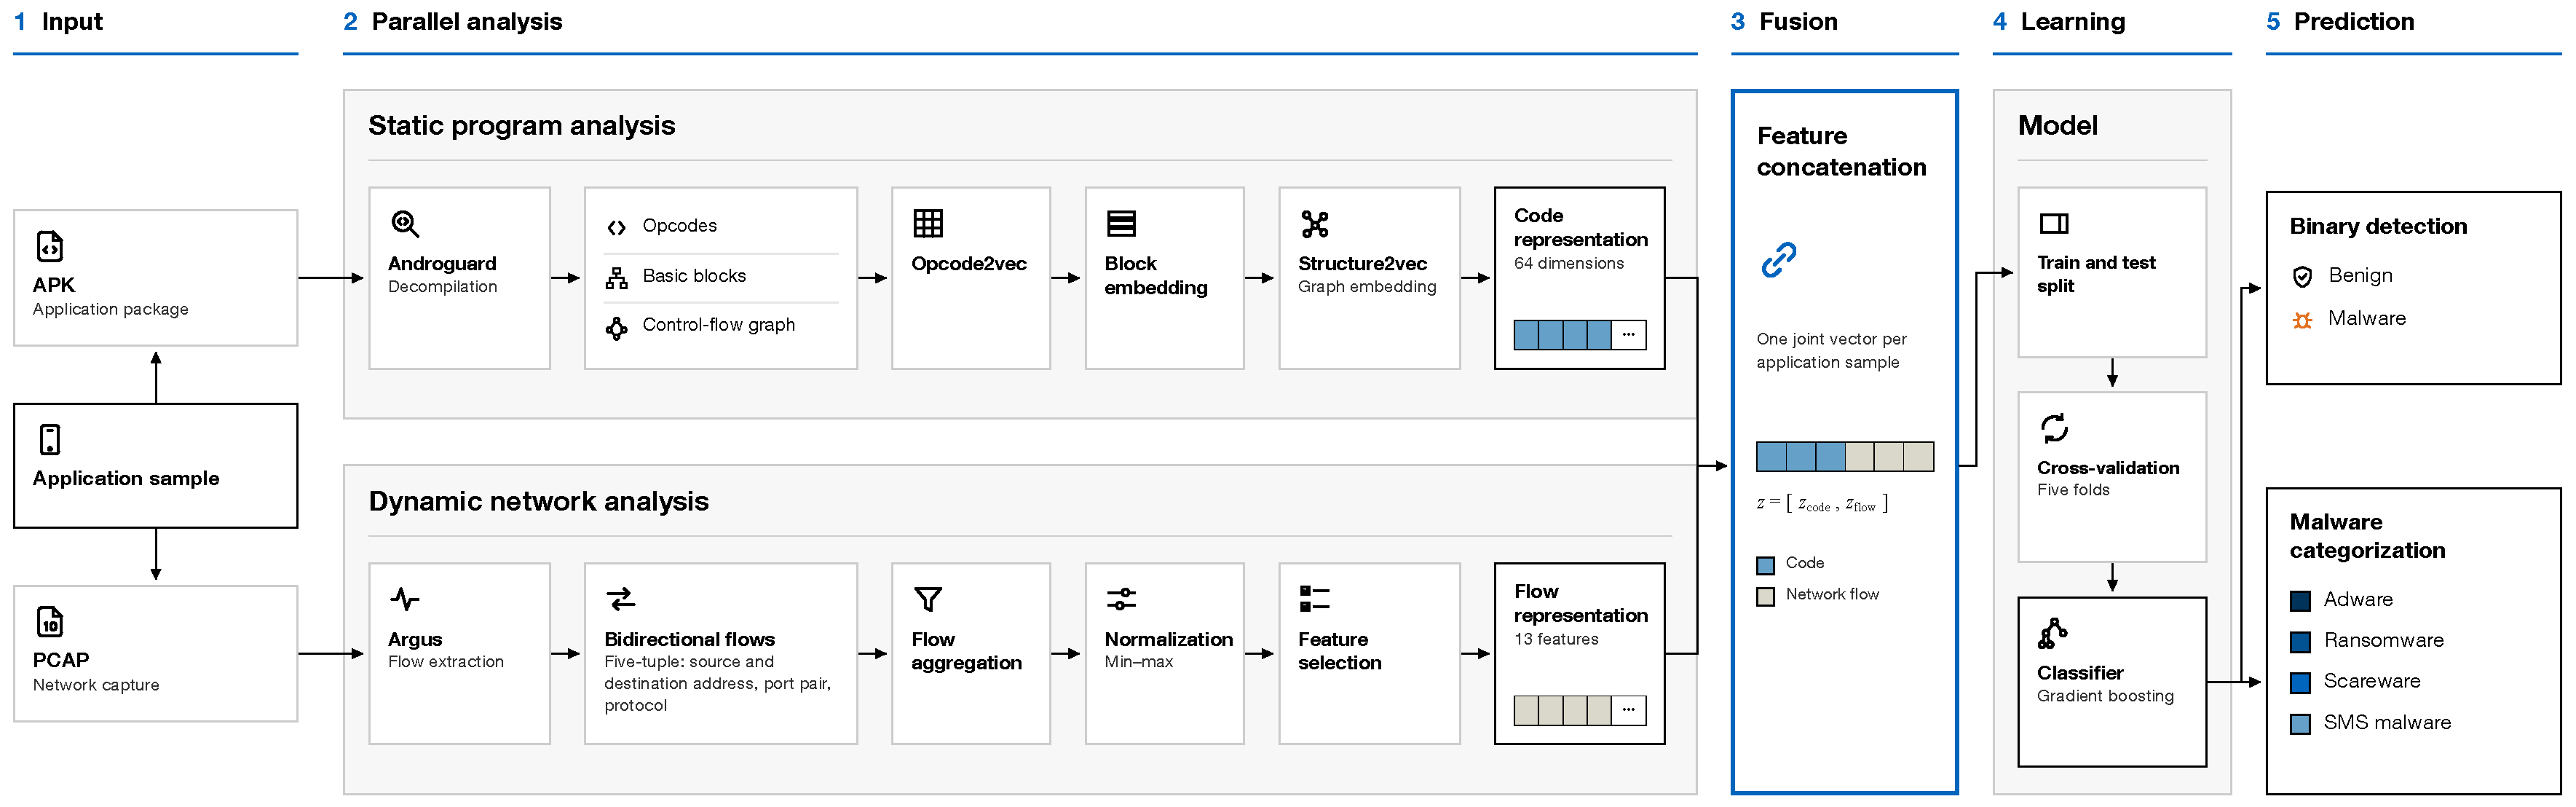
\includegraphics[width=\linewidth]{hybroid-architecture.pdf}
  \caption{The Hybroid architecture. Every application sample provides a pair of inputs: the
  application package and a capture of the traffic it generates~(1). Both are analysed in
  parallel~(2). Androguard decompiles the package into opcodes, basic blocks and a control-flow
  graph, which are embedded into a 64-dimensional code representation, while Argus turns the
  capture into bidirectional flows that are aggregated, normalised and reduced to
  \netfeatures{}~network-flow features. The two representations are concatenated into one joint
  vector per sample~(3), on which a gradient-boosting classifier is trained and
  cross-validated~(4) for binary detection and for categorisation into four malware
  categories~(5). Redrawn by the candidate from the architecture published in
  \cite{norouzian2021hybroid}.}
  \label{fig:hybroid:architecture}
\end{figure}

Three claims are made for the work, and each is stated here in the form the evidence supports
rather than in the form the source publication used. The first is the flow pipeline: network
traffic captured from a real device is reduced to a fixed feature vector per application, through
bidirectional flow records, aggregation, scaling and a selection stage that leaves
\netfeatures{} features. The second is the program-code pipeline: instruction embeddings learned
from a large opcode corpus are composed into method-level vectors, which carry an
application-level function-call graph that a graph embedding converts into a single vector. The
third is the comparison itself, which measures each modality alone and the two together, under
one split, for detection and for category classification. The third depends on the first two and
is what Section~\ref{sec:hybroid:11} rests on.

Two limits on those claims belong here rather than in the limitations section, because they
qualify what is being claimed rather than what was found. The source publication names three
components, \texttt{opcode2vec}, \texttt{function2vec} and \texttt{graph2vec}, of which the
second is never defined anywhere in it and the third names a published method that the work does
not use. This chapter therefore describes the three steps and does not name them. And the
comparison in Section~\ref{sec:hybroid:9} is against four reimplemented systems of unequal
weight, which that section states when it reports the numbers.

The work was published at ISC 2021 \cite{norouzian2021hybroid}, with the candidate first of four
authors and the paper recording that the first two share first authorship. The candidate's own
contribution is stated in Section~\ref{sec:intro:publications}, which the affidavit covers: the
pipeline as a whole and the network-traffic analysis within it are his, as is the framework
through which the dataset was analysed, and he carried out the experiments and wrote the paper.
His contribution to the treatment of the graph data is partial, and this chapter does not present
the program-code pipeline as his own design.

\section{Related Work}
\label{sec:hybroid:2}

Section~\ref{sec:background:android:analysis} distinguishes static, dynamic and hybrid analysis
and reports that roughly one work in ten among surveyed deep-learning defences used both
\cite{liu2023deeplearning}. Section~\ref{sec:background:graphs:pairwise} defines the graph
objects. Neither is repeated here. What follows places \hybroid{} among the systems it was
measured against and among the work that has appeared since.

Static detectors read the application package. Features are drawn from the manifest and from the
code, and the families in use by 2021 were permissions and intents
\cite{arora2014malware, zulkifli2018android}, API calls
\cite{aafer2013droidapiminer, peiravian2013machine}, and structures recovered from the bytecode
\cite{gascon2013structural, li2019android, chen2018android}. DREBIN is the reference point among
them and one of the baselines in Section~\ref{sec:hybroid:9}: it gathers as many such features as
it can, from permissions and hardware requests through API calls to network addresses found in
the code, and embeds them in one vector space in which a linear model can be inspected to say
which features drove a verdict \cite{arp2014drebin}. Its breadth is also where it is exposed,
since the manifest entries and the identifiers a static analyser reads can be rewritten without
altering what the application does \cite{comparetti2010identifying}, which
Section~\ref{sec:background:android:obfuscation} treats in general terms.

A second static family works below the level of identifiers, on the instruction stream itself.
Sequences of opcodes have been used directly as features, with the effectiveness of $n$-grams over
them measured against families of malicious applications \cite{canfora2015effectiveness}, and
convolutional networks have been trained over raw opcode sequences to learn the relevant patterns
rather than to enumerate them in advance \cite{mclaughlin2017deep}. That line is the immediate
precursor of the representation in Section~\ref{sec:hybroid:5}, and the difference is where the
sequence stops. A model over a flat opcode sequence sees the program as one string. The
representation used here keeps the opcode alphabet and then organises it, first into methods and
then into the graph of calls between them.

Graph-based detectors use the structure rather than the identifiers. Adagio hashes neighbourhood
subgraphs of the function-call graph into an explicit feature map, which lets a linear classifier
be trained over graph structure at low cost and lets a verdict be traced back to the code
structures that produced it; it reports detection of 89 per cent of its malware
\cite{gascon2013structural}. It is the second static baseline in Section~\ref{sec:hybroid:9}.
apk2vec learns application embeddings from several graph views at once
\cite{narayanan2018apk2vec}. MaMaDroid takes a different route through the same object,
abstracting each call target to its package or family before modelling transitions between them,
which buys stability against the appearance of unseen methods at the cost of the callee's
identity \cite{onwuzurike2019mamadroid}.

All of these build the object \hybroid{} builds, and what separates them is how a vertex is
described. Adagio's vertex labels are hand-built from categories of instruction, and so are the
attributed control-flow graphs used for similarity between binaries
\cite{xu2017neural, yan2019classifying}. \hybroid{} learns the labels instead
\cite{bengio2013representation}. That choice has since acquired support it did not have at the
time: a benchmark study of graph-based Android classifiers reports that they exceed 94 per cent
accuracy on standard corpora yet lose up to 45 per cent under distribution shift on unseen
variants of known families, and it names structure-only function-call graphs as an inherent
limitation of those benchmarks, because topology alone misses the semantic patterns that
generalisation needs \cite{tran2025quantifying}. That study is a preprint under review. For the
wider design space of graph representation learning applied to malware, one survey covers the
extraction and architecture choices in full \cite{bilot2024survey}.

Dynamic detectors observe behaviour. Two branches exist, one reading system-level activity such
as system calls and API usage, the other reading what crosses the network. \hybroid{} belongs to
the second, which is cheaper to collect than system-call tracing and which exposes the part of an
application's behaviour that a remote operator depends on, since exfiltration and command traffic
have to leave the device to be of use \cite{malik2016credroid, arora2014malware}. Work in this
branch has ranged from rule-based inspection of what an application transmits
\cite{malik2016credroid} to learned models over traffic representations
\cite{wang2017malware, marin2021deepmal}. CICAndMal2017 was built to support it, and its authors
classify Android malware from flow features alone \cite{lashkari2018toward}, which makes their
system the dynamic baseline in Section~\ref{sec:hybroid:9}; they later added API calls to the same
pipeline \cite{taheri2019extensible}.

Granularity is the choice that divides this branch, and it runs from raw packets, which deep
models have been trained on directly \cite{marin2021deepmal}, through individual flows to whole
sessions \cite{wang2017malware}. The choice matters
more than it appears to, because it fixes what a label can attach to.
Section~\ref{sec:hybroid:7} returns to it.

Hybrid systems combine the two, and a systematic review of that literature is available and
replaces an enumeration here \cite{jain2026hybrid}. Two
points from the surrounding literature bear directly on this chapter. Measured under one
protocol, static analysis has proved at least as effective as dynamic analysis and the
combination has measured best \cite{onwuzurike2018family}; that comparison has rarely been
repeated, which is gap~\gapref{2}. And the modality pair used here was taken up again four years
later by HGDetector, which builds a static function-call graph and a network-behaviour graph from
the traffic, fuses them through a graph embedding, and evaluates on the same corpus
\cite{feng2025hgdetector}. Its result is conditional, and the condition is the useful part: the
gain from fusion is reported as roughly 4 per cent where the traffic features already capture an
application's behaviour, and 21 to 26 per cent where they do not. Section~\ref{sec:hybroid:11}
returns to that.

\section{Observation and Threat Model}
\label{sec:hybroid:3}

What a detector can see bounds what it can claim, and Chapters~\ref{chap:hybroid}
and~\ref{chap:hgann} differ in exactly that respect. This section fixes the observation model so
that the two are not read as competing designs.

\hybroid{} observes two things. The first is the Dalvik bytecode recovered from the application
package by a static analyser, from which methods, their instructions and the calls between them
are taken. The second is the traffic the application produces while running on a physical
handset, captured as packets and reduced to bidirectional flow records. Both observations are
made once, offline, before any verdict is given.

Several things are not observed. System calls are outside the model, as is code loaded at
runtime, and so is native code reached through the Java Native Interface. The contents of
encrypted payloads are also outside it, and that limit is measured rather than assumed: across
the four malware categories, the share of flows using TLS runs from 0.00 to 10.89 per cent, which
Section~\ref{sec:hybroid:7} reports and Section~\ref{sec:hybroid:12} takes up as a threat to
validity. The position in which the system is deployed follows from this. It analyses a sample
together with a capture of its traffic, which places it in an analysis pipeline rather than on
the handset.

The adversary is non-adaptive. The malware predates the system by several years and was not
written against this detector, no attacker knowledge is modelled, and no evasion attempt is
made against the trained model. Grey box in the sense fixed in
Section~\ref{sec:background:adversarial} is therefore not claimed here, since that term denotes
a level of attacker knowledge and this evaluation models none.
Section~\ref{sec:hybroid:12} states what follows from that, and what the attacks published since
2025 imply for a pipeline built over a function-call graph.

\section{Dataset and Experimental Protocol}
\label{sec:hybroid:4}

The evaluation uses CICAndMal2017 \cite{lashkari2018toward}, which supplies application packages
together with the traffic each one produced. Benign applications were collected from Google Play
across 2015 to 2017 and malicious ones from VirusTotal and the Contagio archive. The traffic was
captured from three physical handsets rather than from an emulator, with scripted user
behaviour and live accounts on messaging and social platforms, and in three states: immediately
after installation, before a reboot, and after it. Real devices are the reason this corpus was
chosen, since emulator captures do not reproduce the network behaviour of a handset in use.

\begin{table}
  \caption{CICAndMal2017 source-corpus composition. The category counts are recomputed from the
  dataset family listing and differ from the published values of 124, 112, 109 and 101, which do
  not sum to the stated total of 426.}
  \label{tab:hybroid:dataset}
  \centering
  \begin{tabular}{lrrr}
    \toprule
    Class & Families & Samples & Share \\
    \midrule
    Benign        &     & 1,700 & 80.0\,\% \\
    \midrule
    Adware        & 10  &   104 &  4.9\,\% \\
    Ransomware    & 10  &   101 &  4.8\,\% \\
    Scareware     & 11  &   112 &  5.3\,\% \\
    SMS malware   & 11  &   109 &  5.1\,\% \\
    \midrule
    Malware       & 42  &   426 & 20.0\,\% \\
    Total         &     & 2,126 & 100.0\,\% \\
    \bottomrule
  \end{tabular}
\end{table}

Table~\ref{tab:hybroid:dataset} gives the source-corpus composition. The published category rows
sum to 446 against the stated 426, and their percentages sum to 101.0. The recount closes on 426
across 42 families. The 47 exclusions are not identified by class. The dataset documentation
reports 5,065 benign applications installed, and the 1,700 used here is the number of benign
captures the distribution provides.

The source corpus pairs 2,126 applications with their traffic. Both analyses excluded the 47
graph-extraction failures and used the remaining 2,079 applications.
Model selection and evaluation use five-fold cross-validation with the results averaged over the
folds. Implementation used Python with
scikit-learn, TensorFlow and Keras, on a server with 32 cores, 128\,GB of memory and a 16\,GB
accelerator. Accuracy, precision, recall, the $F_1$ score and the area under the ROC curve
are reported, with $F_1$ preferred under the class imbalance Table~\ref{tab:hybroid:dataset}
shows. The averaging convention behind those metrics is not stated in the source, which
Section~\ref{sec:hybroid:9} returns to.

A second and larger experiment exercised the program-code pipeline alone. It used 45,592
malicious and 90,313 benign applications drawn from AndroZoo, VirusShare and VirusTotal, which is
135,905 samples at a malicious share of 33.5 per cent, split at random into 80 per cent for
training and 20 per cent for testing, and it reached an accuracy of 95.0 per cent with an $F_1$
score of 96.0 per cent. It is reported here as a check that the program-code pipeline scales
beyond a corpus of a few thousand samples. It is not a time-aware evaluation, and
Section~\ref{sec:background:evaluation} sets out why that distinction matters
\cite{pendlebury2019tesseract}.

\section{Opcode and Method-Level Representation}
\label{sec:hybroid:5}

Dalvik instructions carry an operation and its operands. Only the operation is embedded here, and
the reason is that the operands are register references whose values depend on the runtime that
executes them \cite{aosp2026dalvikbytecode, aosp2026art}, so they cannot be enumerated across
applications in the way a vocabulary must be. The operation, by contrast, is drawn from a fixed
alphabet of 216 opcodes, and samples within one malware family that share a malicious pattern
share the operations that implement it.

The embedding is learned rather than assigned. Each opcode is mapped to a real-valued vector by
the skip-gram formulation of word2vec, in which the model is trained to predict the operations
surrounding a given one \cite{mikolov2013distributed}. Training used a corpus of 18,240,542
opcodes extracted from applications drawn from AndroZoo. Two opcodes that occur in similar
positions therefore receive similar vectors, so the representation encodes the company an
operation keeps rather than an arbitrary index assigned to it, which is what a one-hot encoding
over the same alphabet would give.

\begin{figure}
  \centering
  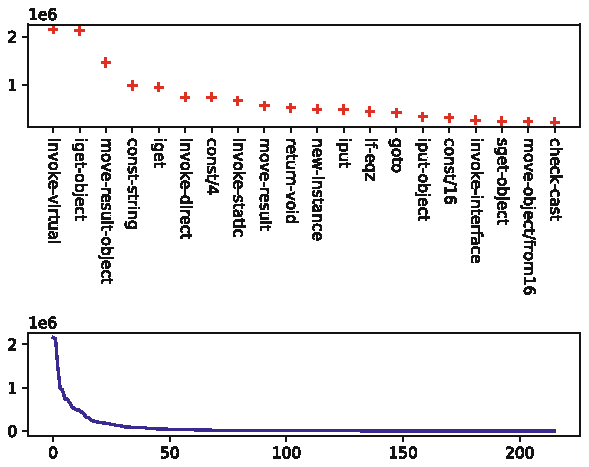
\includegraphics[width=0.72\linewidth]{hybroid-opcode-powerlaw.pdf}
  \caption{Opcode frequency across the pre-training corpus. The upper panel names the twenty most
  common operations, and the lower panel plots all 216 in rank order, where the shape of the decay
  is the property the embedding relies on. Reproduced from the candidate's own publication
  \cite{norouzian2021hybroid}, as is Figure~\ref{fig:hybroid:correlation}.}
  \label{fig:hybroid:powerlaw}
\end{figure}

Borrowing a technique from language modelling needs a reason beyond convenience, and the
distribution of the alphabet supplies it. Counting opcodes across the corpus shows the twenty
most frequent following a power law, as Figure~\ref{fig:hybroid:powerlaw} shows, which is the
property that holds for words in natural language, which is the setting the skip-gram objective
was built for \cite{mikolov2013distributed}. The alphabet also behaves better
here than in the setting the technique came from. Natural language has an open vocabulary and a
model trained on one corpus meets unseen words in another; the Dalvik instruction set is closed
at 216 operations for the format the corpus was drawn from, so an embedding trained once covers
the applications the analyser reads, and the unseen-token case that troubles language models does
not arise in the same way. This is what makes a transductive method acceptable in a
detector that must generalise, and Section~\ref{sec:hybroid:6} returns to the point.

Discarding the operands has a cost, and it is specific rather than general. Every call
instruction receives the same vector whatever it invokes, because the target sits in the operand
field \cite{haq2021survey}. This is worth stating plainly at the point where the representation is
built, because the object built next is a graph whose edges are exactly those call targets. The
vertex features and the edge set are therefore recovered by two passes over the bytecode that
share no information, and the vertex features are blind to the structure that the edges record.

Above the instruction, a method is represented by combining the vectors of the instructions it
contains. The source publication calls this a basic-block embedding and gives it as a weighted
mean, $\tilde{f} = \sum_{i} w_i x_i / \sum_i w_i$, where $x_i$ is the $l$-dimensional embedding of
the $i$-th opcode. Two things about that definition are carried forward as they stand rather than
tidied. The weights $w_i$ are not specified anywhere in the source, which leaves the mean
undefined. And the formula is written over the $n$ opcodes of a function while the prose around it
calls the result the embedding of a basic block, so the two do not describe the same object.
Section~\ref{sec:hybroid:12} records both.

What the vector is used for is stated unambiguously, and that is what
Section~\ref{sec:hybroid:6} needs. It becomes the feature attached to a vertex of the method's
control-flow graph, whose vertices are basic blocks.

\section{Program-Graph Representation}
\label{sec:hybroid:6}

Section~\ref{sec:background:graphs:pairwise} defines the control-flow graph, the function-call
graph, and the composition in which per-method embeddings become the vertex features of a
call graph. \hybroid{} builds the composition. Control-flow graphs are extracted per method with
Androguard \cite{desnos2012android}, each one is reduced to a single vector, and those vectors
describe the vertices of the application's function-call graph, which is the object the
classifier consumes. Both terms are needed, and they are not interchangeable.

\begin{figure}
  \centering
  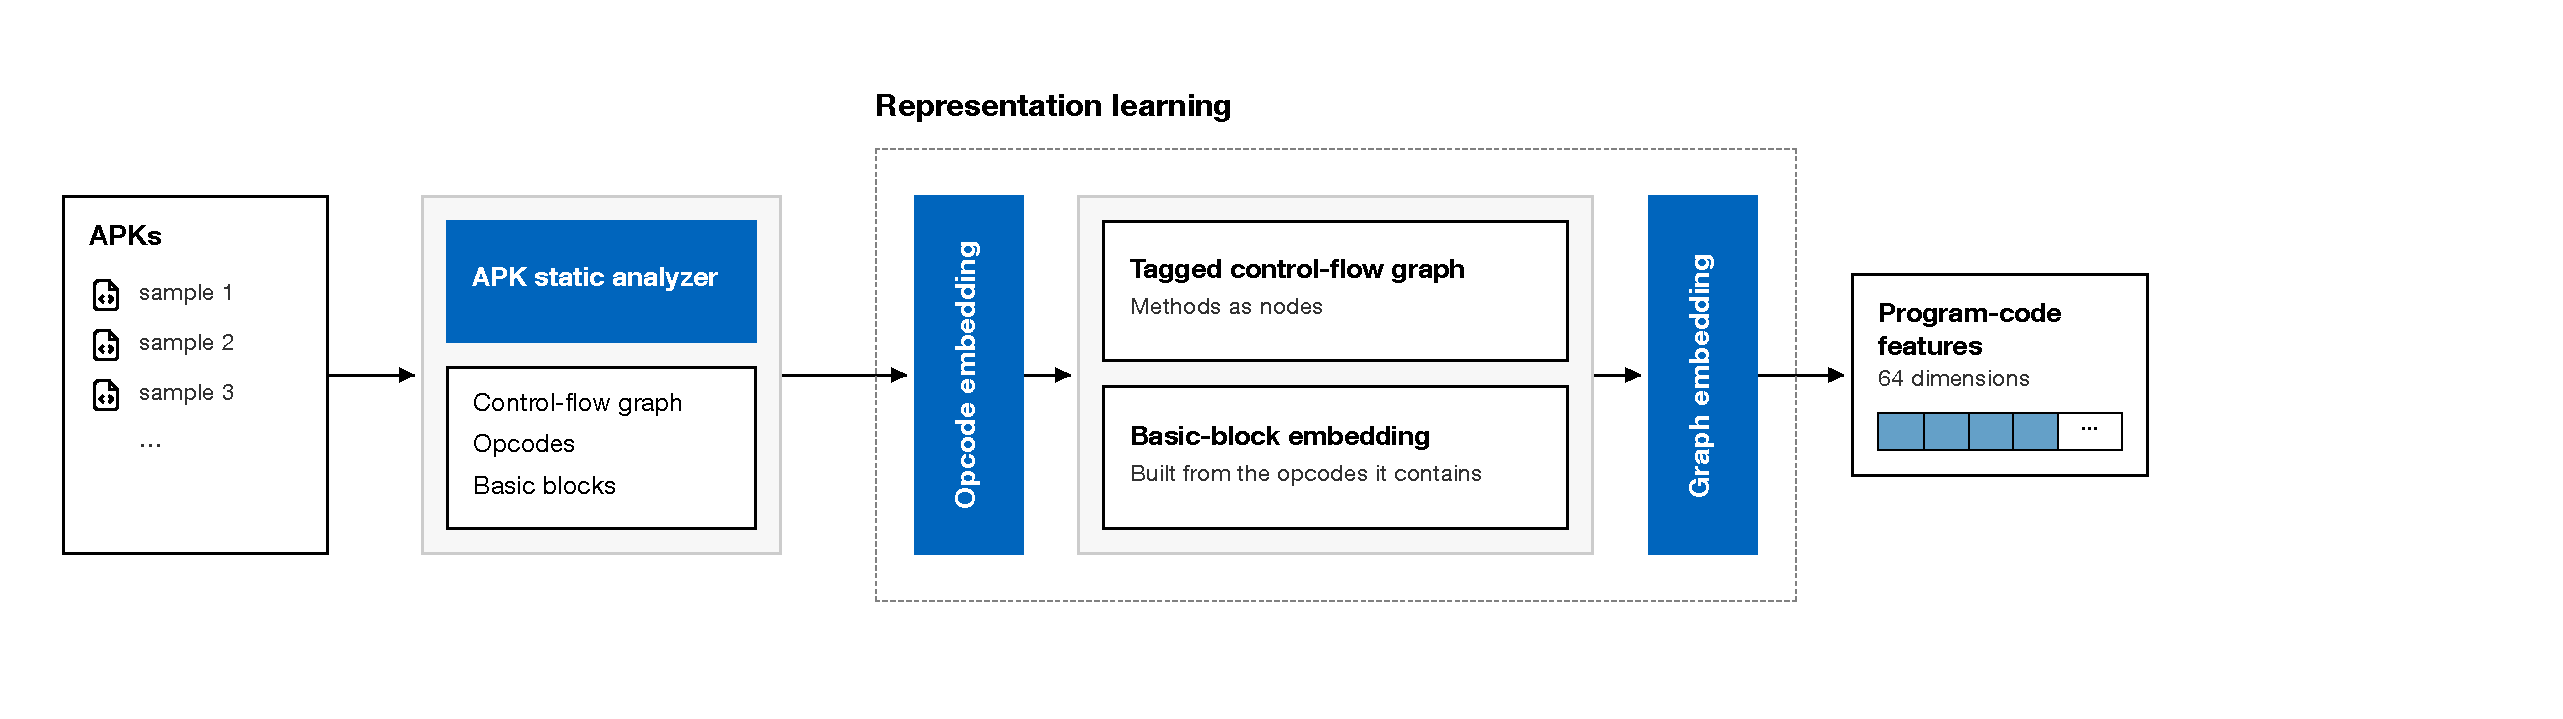
\includegraphics[width=\linewidth]{hybroid-code2vec.pdf}
  \caption{The program-code branch. The static analyzer extracts the control-flow graph, opcodes
  and basic blocks from each APK. Opcodes are embedded first, every method is represented from
  the tagged control-flow graph of the basic blocks it contains, and a graph embedding reduces
  the resulting function-call graph to a single 64-dimensional feature vector. Redrawn by the
  candidate from the arrangement published in \cite{norouzian2021hybroid}.}
  \label{fig:hybroid:code2vec}
\end{figure}

Figure~\ref{fig:hybroid:code2vec} sets out the branch as a whole. Two properties of that object
bound what any detector built on it can claim, and both are set out
in Section~\ref{sec:background:graphs:pairwise}. A call graph recovered without running the
program over-approximates, because the analysis admits edges that no execution takes. It also
under-approximates, since calls made through reflection, through code loaded at runtime or through
native libraries leave no edge for a static analyser to find, and Section~\ref{sec:hybroid:3}
records that all three are outside what is observed here. The object is in that sense an artefact
of the analyser rather than a property of the program, since which edges are found depends on the
toolkit and on how the component lifecycle is modelled. Neither property is
peculiar to this work. Both mean that the structure being classified is a static estimate of the
program's shape, and Section~\ref{sec:hybroid:12} states what follows when an adversary is
allowed to influence that estimate.

Reducing the graph to a vector could be done by counting substructures, which is what the kernel
methods discussed in Section~\ref{sec:hybroid:2} do \cite{gascon2013structural}. The route taken
here instead propagates information along the edges and lets the features of a vertex be shaped
by its neighbourhood.

The reduction from a graph to a vector uses structure2vec \cite{dai2016discriminative}. A
$p$-dimensional vector $\mu_v$ is attached to each vertex $v$ and initialised at random, then
updated for $T$ rounds by a function of the vertex's own features and the sum of its neighbours'
current vectors,
%
\begin{equation}
  \mu_v^{(t+1)} = F\!\left(x_v, \sum_{u \in N(v)} \mu_u^{(t)}\right), \qquad \forall v \in V,
  \label{eq:hybroid:meanfield}
\end{equation}
%
with $F$ realised as
%
\begin{equation}
  F\!\left(x_v, \sum_{u \in N(v)} \mu_u^{(t)}\right)
  = \tanh\!\left(W_1 x_v + \sigma\!\left(\sum_{u \in N(v)} \mu_u^{(t)}\right)\right),
  \label{eq:hybroid:update}
\end{equation}
%
where $W_1$ is trainable and $\sigma$ is an $n$-layer fully connected network,
%
\begin{equation}
  \sigma(l) = P_1\,\mathrm{ReLU}\!\left(P_2 \cdots \mathrm{ReLU}(P_n l)\right).
  \label{eq:hybroid:sigma}
\end{equation}
%
After $T$ rounds the vertex vectors are averaged and transformed by a second trainable matrix,
which yields one vector per graph. This is the operator
Section~\ref{sec:background:learning:messagepassing} describes in words, instantiated on the
graphs built here. The number of rounds fixes how far information travels: after $T$ updates a
vertex has been reached by everything within $T$ steps of it, so $T$ sets the size of the
neighbourhood any single vertex vector summarises. Averaging at the end rather than summing keeps
the result comparable across graphs of different sizes, which matters when applications differ by
orders of magnitude in how many methods they contain.

One step in this pipeline is not specified in the source publication, and the chapter states so
rather than supplying a plausible reconstruction. Equations~\ref{eq:hybroid:meanfield}
to~\ref{eq:hybroid:sigma} are applied at the level of a method's control-flow graph, and the
averaging inside that procedure pools the basic blocks of one method. The step that combines the
resulting per-method vectors into the single 64-dimensional vector standing for the whole
application is named as the third step of the pipeline and is specified by no equation. Nothing in
the source refers to a caller or a callee in symbols, so the composition is stated there as a
design and is reproduced here as one.

A note on transduction closes the description. The opcode embedding is transductive, since
word2vec needs the whole alphabet at training time. That alphabet is the fixed Dalvik instruction
set, so the requirement is met by construction rather than by assumption about the corpus. The
graph embedding is inductive, and graphs in the test partition are unseen when it is trained.

\section{Network-Flow Representation}
\label{sec:hybroid:7}

\begin{figure}
  \centering
  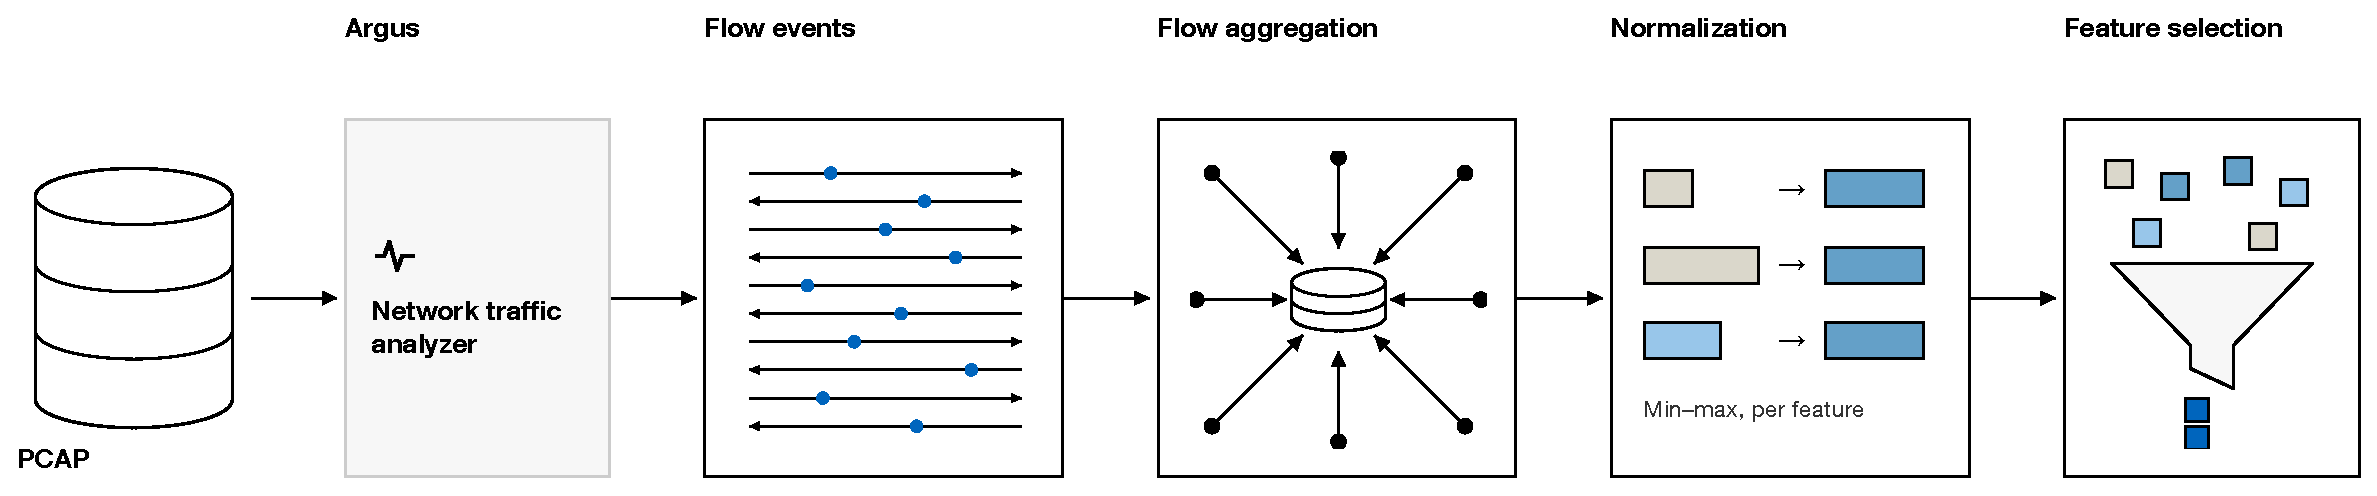
\includegraphics[width=\linewidth]{hybroid-dynamic.pdf}
  \caption{The network branch. Argus reduces a raw capture to bidirectional flow events, the
  events belonging to one application are aggregated into a single record, every attribute is
  normalised to a common range, and feature selection retains the \netfeatures{}~most informative
  features. Redrawn by the candidate from the arrangement published in
  \cite{norouzian2021hybroid}.}
  \label{fig:hybroid:dynamic}
\end{figure}

Section~\ref{sec:background:networks:flows} sets out the flow abstraction.
Figure~\ref{fig:hybroid:dynamic} gives the branch. Here the captures are processed with Argus \cite{qosient2026argus}, which produces bidirectional records grouped by the
usual five-tuple of source and destination address, source and destination port, and protocol,
and reports roughly forty statistics for each record. Two of those statistics are categorical,
the direction of the transaction and the state flags, and both are one-hot encoded; the rest are
numeric.

An application produces many flows, and the representation reduces them to one record. The values
of each feature are averaged across all flow events belonging to one capture, which yields a
single feature vector per application and matches the granularity of the program-code vector so
that the two can be combined. Two consequences follow and neither is stated in the source
publication. The label attaches to the application rather than to any individual flow, which
avoids the assumption that every flow emitted by a malicious application is itself malicious.
Against that, averaging discards the order and the timing of the capture, and a small number of
malicious flows is averaged together with whatever background traffic the handset produced during
the same window.

The averaged features are scaled to the unit interval by min-max normalisation, on the ground
that features whose ranges differ by orders of magnitude would otherwise contribute unequally to
any distance computed over them. That rationale applies to the two learners which were tried and
dropped rather than to the three reported in Section~\ref{sec:hybroid:8}, since a tree is
unaffected by any monotone rescaling of a feature. The source publication states that standard
scaling was considered and rejected.

\begin{table}
  \caption{The \netfeatures{} network-flow features retained after selection, grouped by the kind
  of quantity each one measures.}
  \label{tab:hybroid:flowfeatures}
  \centering
  \begin{tabular}{ll}
    \toprule
    Kind & Features \\
    \midrule
    Volume and duration & mean record duration, total bytes, source bytes \\
    Transport state     & destination TCP window, source loss and retransmission flag, \\
                        & destination out-of-order flag, transaction direction \\
    Path and service    & source and destination TTL, source and destination TOS byte \\
    Connection identity & source and destination TCP base sequence number \\
    \bottomrule
  \end{tabular}
\end{table}

Selection reduced the roughly forty statistics to the \netfeatures{} listed in
Table~\ref{tab:hybroid:flowfeatures}, using Pearson correlation, an extremely randomised trees
estimator and a univariate test that keeps the highest-scoring features. Redundancy among the
survivors was checked with Kendall's correlation, shown in
Figure~\ref{fig:hybroid:correlation}. The grouping in the table is this chapter's
addition, and it is there because the four groups do not have equal standing as descriptions of
application behaviour. Volume, duration and transport state are produced by what the application
does. The remaining two groups are not: the TTL reflects the path and the operating system of the
endpoint, the TOS byte is set by few stacks and is commonly zero, and the TCP base sequence
numbers are required to be unpredictable per connection and so cannot carry behaviour at all.
Section~\ref{sec:hybroid:12} takes this up, together with a published audit of the same feature
family in a different corpus.

\begin{figure}
  \centering
  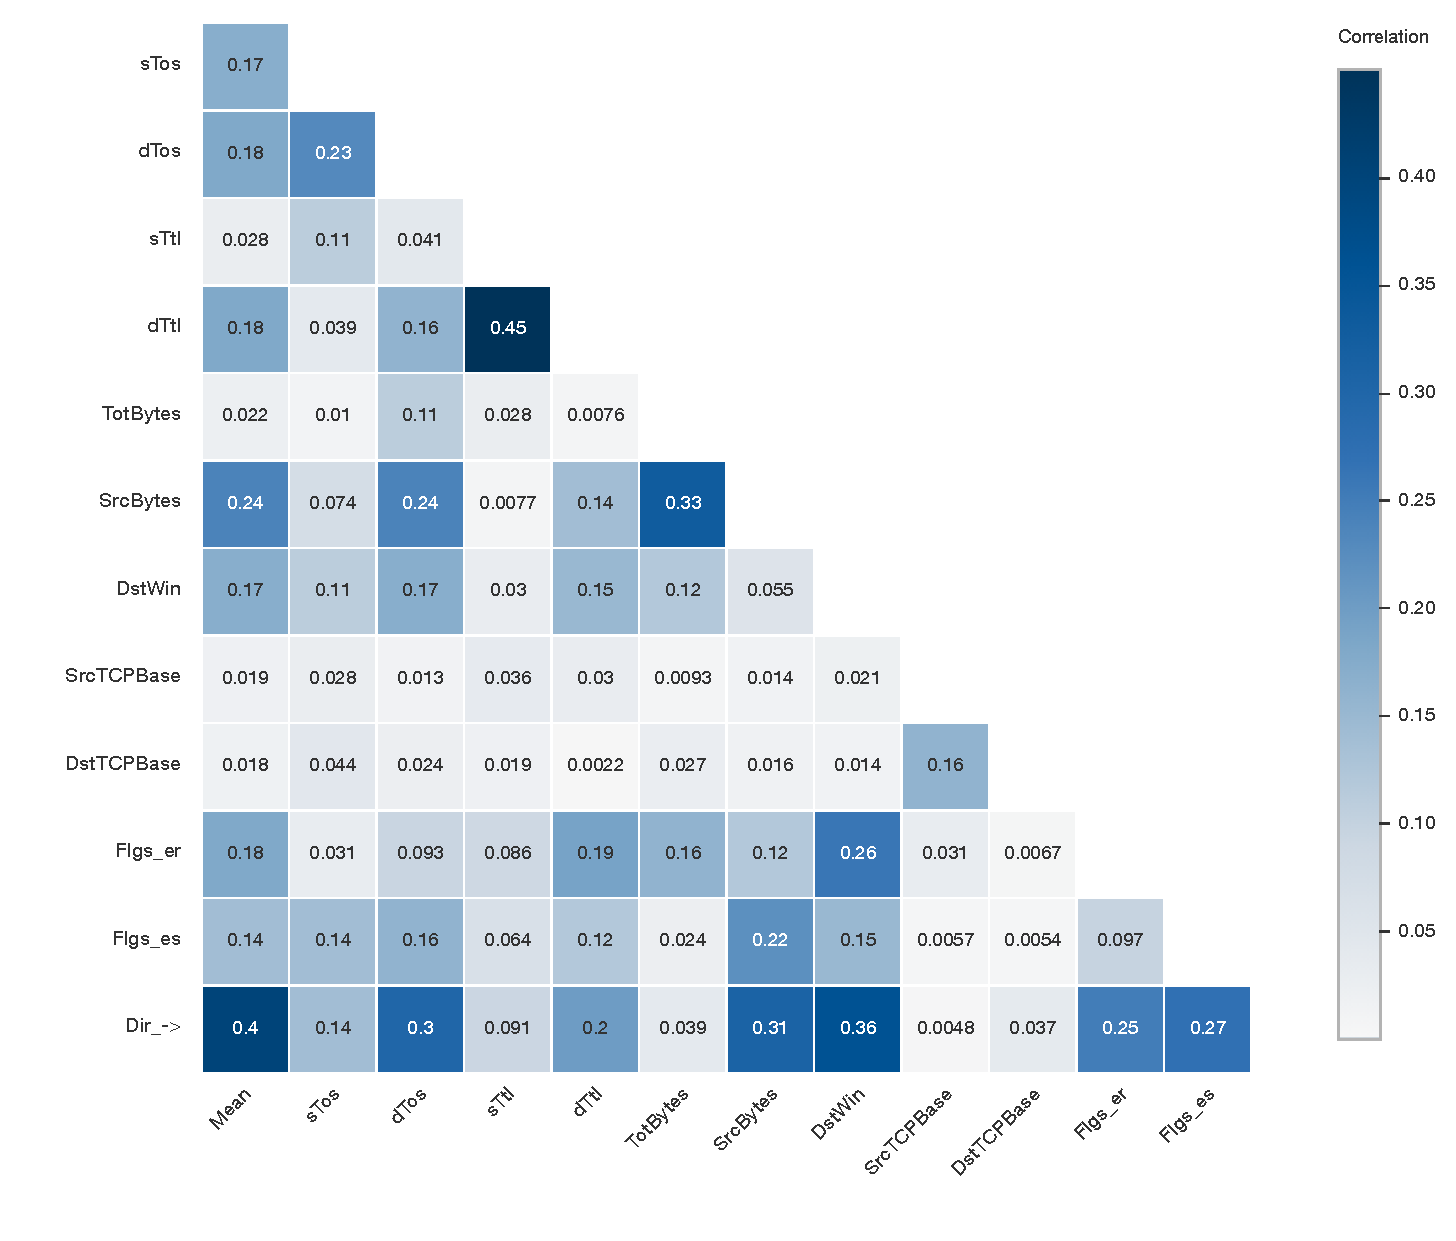
\includegraphics[width=0.82\linewidth]{hybroid-flow-correlation.pdf}
  \caption{Kendall correlation among the retained flow features, used to check that the selected
  features are not redundant with one another.}
  \label{fig:hybroid:correlation}
\end{figure}

A separate observation concerns what the traffic carried, and
Table~\ref{tab:hybroid:protocols} records it. Cleartext HTTP accounts for between 29.22 and 61.38
per cent of flows across the four malware categories, and TLS for between nothing at all and
10.89 per cent. The remainder, which runs from 27.73 to 70.78 per cent depending on the category, is neither named nor characterised in the source publication. \begin{table}
  \caption{Share of flows by protocol, per malware category. The two columns do not sum to 100
  per cent and the source publication does not say what the remainder is.}
  \label{tab:hybroid:protocols}
  \centering
  \begin{tabular}{lrrr}
    \toprule
    Category & HTTP & TLS & Unaccounted \\
    \midrule
    Adware      & 52.00\,\% &  8.00\,\% & 40.00\,\% \\
    Ransomware  & 29.22\,\% &  0.00\,\% & 70.78\,\% \\
    Scareware   & 61.38\,\% & 10.89\,\% & 27.73\,\% \\
    SMS malware & 52.20\,\% & 10.28\,\% & 37.52\,\% \\
    \bottomrule
  \end{tabular}
\end{table}

Flow-level features
were chosen over inspection of payloads for reasons of privacy and cost, and that choice has
become the only available one since: beyond transport encryption, a substantial share of
applications encrypt content themselves before sending it, with one measurement of 12,598
applications finding 22.92 per cent doing so and most of those transmitting device-identifying
information \cite{pourali2022hidden}.

\section{Multimodal Fusion and Classification}
\label{sec:hybroid:8}

Two classifiers appear in this pipeline and they do different work, which is worth separating
before either is described, because a reader who meets both without warning will take one of them
for a mistake.

The first sits at the end of the program-code branch. A two-layer fully connected network takes
the graph vector and is trained to discriminate, with malicious samples labelled $+1$, benign
samples $-1$, and a decision taken at zero. Its purpose is to fit the parameters of the
representation, since the matrices in Equations~\ref{eq:hybroid:meanfield}
to~\ref{eq:hybroid:sigma} have to be learned against some objective and detection is the
objective available. What leaves the branch is the 64-dimensional vector, and the network that
produced it plays no further part.

One consequence deserves stating, because it bears on Section~\ref{sec:hybroid:10}. The objective
that fits the program-code representation is binary, and the same representation is then used for
the five-class task. A representation tuned to separate malicious from benign need not be equally
informative about which kind of malicious an application is, and nothing in the source
publication indicates that the embedding was refitted for the second task. Whether the
categorisation results would improve under a representation fitted to that objective was not
measured.

The second classifier acts on both modalities. The 64-dimensional program-code vector and the
\netfeatures{} flow features are taken together as one input, on which a supervised learner is
trained for detection and, separately, for category classification. The source publication
describes the two groups as forming a single input vector and does not name the operator that
combines them, so this chapter does not name it either. The proportions of that input are however
fixed by the two branch designs and they are uneven: 64 of the 77 dimensions come from the
program code, so the static half supplies roughly five dimensions in every six. No weighting is
applied to correct for this, and none is reported as having been considered.

Five learners were tried. Support vector machines and naive Bayes performed worst and were
dropped, leaving a decision tree, a random forest and a gradient boosting classifier, which are
the three reported throughout Sections~\ref{sec:hybroid:9} to~\ref{sec:hybroid:11}. No figures
are given for the two that were dropped, so the margin by which they were rejected is not on
record. The three that remain are tree-based learners of increasing capacity, which is convenient for
the comparison in Section~\ref{sec:hybroid:11}: the decision tree fits axis-aligned splits on a
single model, the random forest averages over many such models, and gradient boosting fits them
in sequence against the residual of what came before. Reading the three together therefore says
something about how much capacity the fused representation needs, and not only about which
learner wins.

Combining the modalities at the level of features, rather than training a model on each and
combining their decisions, is a design choice, and it was the ordinary one at the time. Its
consequences were not visible in 2021. Section~\ref{sec:hybroid:11} reports what the measurements
here show and sets them beside the evidence that has accumulated since.

\section{Binary Detection Results}
\label{sec:hybroid:9}

\begin{table}
  \caption{Detection compared with four reimplemented systems, read from the published figures.
  The four systems differ considerably in weight: DREBIN is a full conference paper, Adagio and
  CIC 2017 are papers of ten and seven pages, and the SVM entry is a two-page poster. The reported
  performance values come from Figures~6 and~7 of \cite{norouzian2021hybroid}.}
  \label{tab:hybroid:baselines}
  \centering
  \begin{tabular}{lrrrrr}
    \toprule
    System & Accuracy & $F_1$ & Recall & Precision & AUC \\
    \midrule
    SVM \cite{dai2015svm}                & 0.939 & 0.860 & 0.856 & 0.865 & 0.876 \\
    DREBIN \cite{arp2014drebin}          & 0.954 & 0.867 & 0.873 & 0.861 & 0.961 \\
    Adagio \cite{gascon2013structural}   & 0.893 & 0.932 & 0.913 & 0.953 & 0.867 \\
    CIC 2017 \cite{lashkari2018toward}   & 0.876 & 0.872 & 0.878 & 0.871 & 0.914 \\
    \midrule
    \hybroid{}                           & 0.970 & 0.969 & 0.970 & 0.970 & 0.996 \\
    \bottomrule
  \end{tabular}
\end{table}

Table~\ref{tab:hybroid:baselines} reports the comparison published for binary detection
\cite{norouzian2021hybroid}. \hybroid{} has the highest point value in each column. Two
qualifications accompany the comparison because they affect how the values can be read.

The first concerns the comparison set. The four systems are not of equal weight, and the SVM
entry is a two-page poster \cite{dai2015svm}, so the phrase state of the art would carry more
than the table supports.

The second qualification concerns the metrics. For a binary problem
in which accuracy is computed over the whole test set and precision and recall over the malicious
class, the three quantities determine the malicious share $p$ of that set through
$\mathrm{acc} = 1 - p\left[(1-R) + R(1-P)/P\right]$. Solving for each row of
Table~\ref{tab:hybroid:baselines} gives 22.0 per cent for the SVM entry, 17.2 for DREBIN, and
81.0, 49.2 and 50.0 per cent for Adagio, CIC 2017 and \hybroid{}. Depending on the labels of the 47
exclusions, the evaluated malware share lies between 18.2 and 20.5 per cent. The last three values
remain incompatible with that interval. The source publication does not state which averaging
convention produced its figures, and no raw result survives against which to check. The chapter
therefore preserves the published values and does not treat their differences as estimates made
under one documented metric convention.

\begin{figure}[t]
  \centering
  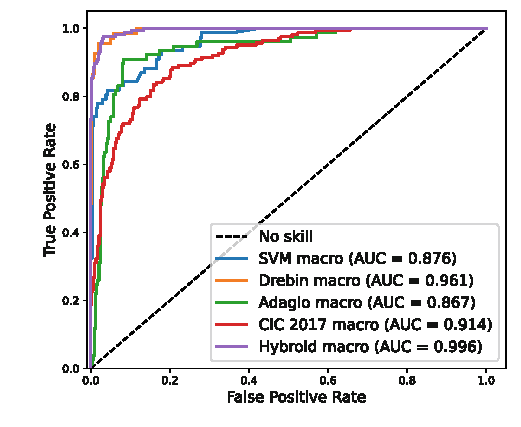
\includegraphics[width=0.72\linewidth]{hybroid-detection-roc.pdf}
  \caption{Receiver operating characteristic curves for binary malware detection, reproduced
  from the published vector content of Figure~7 in \cite{norouzian2021hybroid}. The source labels the curves as macro
  averages and reports the AUC values in the legend. It provides neither a selected operating
  threshold nor fold-level variation.}
  \label{fig:hybroid:detection-roc}
\end{figure}

Figure~\ref{fig:hybroid:detection-roc} shows the corresponding threshold curves. \hybroid{} has
the largest reported AUC at 0.996, followed by DREBIN at 0.961. The dynamic CIC 2017 system has an
AUC of 0.914, ahead of the SVM and Adagio entries despite its lower accuracy in
Table~\ref{tab:hybroid:baselines}. The metric therefore changes the ordering of the baselines.
The AUCs summarise ranking across thresholds, while the paper reports no threshold at which the
detector would operate. It also supplies no fold-level curves or confidence intervals, so the
differences remain descriptive point estimates \cite{norouzian2021hybroid}.

Read by modality, three of the four baselines are static and one is dynamic. The comparison still
mixes the implementation choices of separate systems with the observation modality, so it cannot
isolate a modality effect. Section~\ref{sec:hybroid:11} uses the within-system comparison for that
purpose.

\begin{figure}[t]
  \centering
  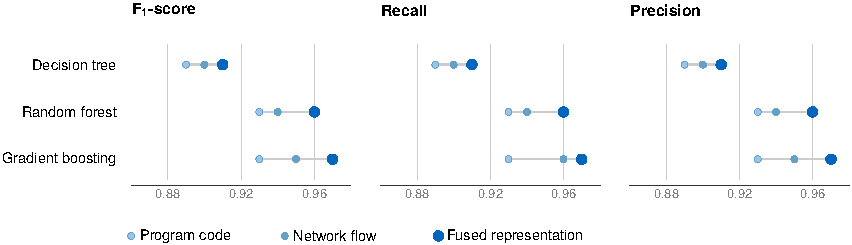
\includegraphics[width=\linewidth]{hybroid-detection-classifiers.pdf}
  \caption{Binary detection by learner and observation modality, with each reported metric in its
  own panel. Every row carries one marker per modality, joined by a rule spanning the values it
  reports. The values are the five-fold means printed to two decimal places in Figure~8 of
  \cite{norouzian2021hybroid}, checked against the bar geometry of that figure. The score axis is
  truncated to 0.86--0.98, the interval those values occupy. No fold-level scores are published,
  so the figure carries no error bars. Redrawn by the candidate.}
  \label{fig:hybroid:detection-classifiers}
\end{figure}

Figure~\ref{fig:hybroid:detection-classifiers} separates the learner comparison from the external
baselines. Gradient boosting on the fused representation reaches 0.97 on all three reported
metrics. Random forest reaches 0.96, while the decision tree reaches 0.91. Network flow alone has
a higher point value than program code alone for each learner. Under program code alone, random
forest and gradient boosting both report 0.93 for $F_1$, recall and precision. Gradient boosting
therefore has the highest fused result, as the paper states, while its program-code result ties
with random forest at the published precision \cite{norouzian2021hybroid}.

At two-decimal precision, $F_1$, recall and precision coincide in eight of the nine
configurations. The remaining configuration is gradient boosting over network flow, for which
recall is 0.96 and the other two values are 0.95. Micro-averaging would make the three metrics
equal by construction, and rounding could also hide small differences. The paper does not state
the averaging convention and provides no raw predictions, so neither explanation can be selected
from the surviving evidence \cite{norouzian2021hybroid}.

\section{Malware-Category Classification}
\label{sec:hybroid:10}

The second task assigns each sample to one of five mutually exclusive classes, the four malware
categories of Table~\ref{tab:hybroid:dataset} together with the benign class. The source
publication calls this multi-label classification throughout; it is multi-class classification
with a single label per sample, and this chapter uses the latter term
\cite{norouzian2021hybroid}.

\begin{figure}[t]
  \centering
  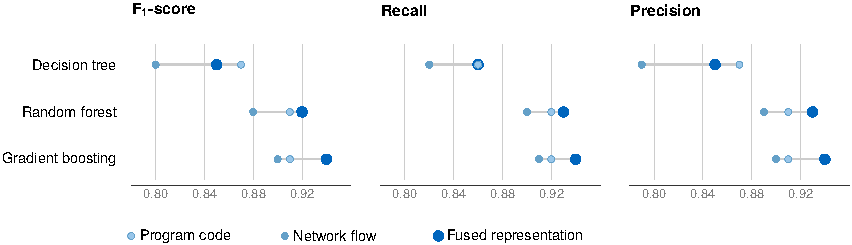
\includegraphics[width=\linewidth]{hybroid-categorisation-classifiers.pdf}
  \caption{Five-class malware-category classification by learner and observation modality, drawn
  on the same plan as Figure~\ref{fig:hybroid:detection-classifiers}. The score axis is truncated
  to 0.78--0.96, because this task occupies a lower interval. The values are the five-fold means
  printed to two decimal places in Figure~9 of \cite{norouzian2021hybroid}, checked against the
  bar geometry of that figure. Decision-tree recall is 0.86 for program code and for the fused
  representation, so those two markers are drawn concentrically. No fold-level scores are
  published, so the figure carries no error bars. Redrawn by the candidate.}
  \label{fig:hybroid:categorisation-classifiers}
\end{figure}

Figure~\ref{fig:hybroid:categorisation-classifiers} gives the category-classification results.
Gradient boosting on the fused representation reaches 0.94 on all three metrics. Random forest
follows at 0.92 for $F_1$ and 0.93 for recall and precision. The decision-tree result differs: the
fused representation reaches 0.85 for $F_1$ and precision, below the program-code values of 0.87,
while recall is equal at 0.86. The paper's general statement that combined features give the best
performance therefore has one exception in its own reported figure
\cite{norouzian2021hybroid}.

Table~\ref{tab:hybroid:perclass} gives the area under the ROC curve for each class, for the
gradient boosting classifier on the combined vector. The macro average of 0.976 is reported as a
macro accuracy in the source publication, which its own figure legend contradicts; it is an
average of areas under the curve \cite{norouzian2021hybroid}.

\begin{table}
  \caption{Area under the ROC curve per class, gradient boosting on the combined representation,
  with the pre-exclusion counts of Table~\ref{tab:hybroid:dataset}. Values are read from Figure~10
  of \cite{norouzian2021hybroid}.}
  \label{tab:hybroid:perclass}
  \centering
  \begin{tabular}{lrr}
    \toprule
    Class & Samples & AUC \\
    \midrule
    Benign        & 1,700 & 0.995 \\
    Ransomware    &   101 & 0.991 \\
    Scareware     &   112 & 0.979 \\
    Adware        &   104 & 0.963 \\
    SMS malware   &   109 & 0.946 \\
    \midrule
    Macro average &       & 0.976 \\
    \bottomrule
  \end{tabular}
\end{table}

\begin{figure}[t]
  \centering
  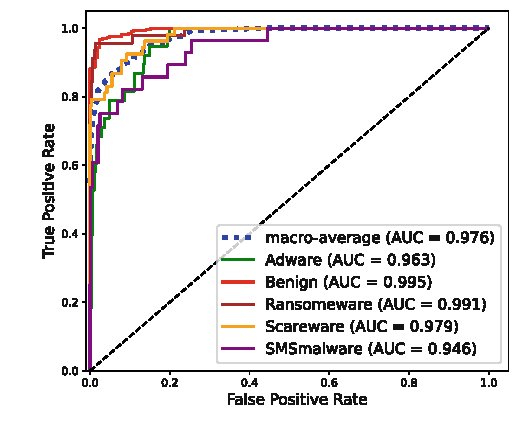
\includegraphics[width=0.72\linewidth]{hybroid-categorisation-roc.pdf}
  \caption{Per-class receiver operating characteristic curves for gradient boosting on the fused
  representation, reproduced from the published vector content of Figure~10 in
  \cite{norouzian2021hybroid}. The legend
  reports a macro-average AUC of 0.976 and the AUC of each class. The paper provides no selected
  operating threshold or fold-level variation.}
  \label{fig:hybroid:categorisation-roc}
\end{figure}

Figure~\ref{fig:hybroid:categorisation-roc} preserves the threshold curves from which the AUC
values in Table~\ref{tab:hybroid:perclass} were read. Benign and ransomware have the largest
reported areas, 0.995 and 0.991. SMS malware has the smallest at 0.946. These values measure class
ranking across thresholds. They do not provide the per-class precision and recall at the decision
rule used for the five-class result, which the paper does not report
\cite{norouzian2021hybroid}.

The averaging convention for the global precision, recall and $F_1$ values is also unstated.
Benign applications remain the majority after the exclusions, so the reported value of 0.94
cannot be interpreted as equal performance across the five classes. Per-class precision and
recall, the fold-level values, and any dispersion measure are unavailable in the paper
\cite{norouzian2021hybroid}.

\section{Modality Comparison}
\label{sec:hybroid:11}

This section answers RQ2. Figures~\ref{fig:hybroid:detection-classifiers}
and~\ref{fig:hybroid:categorisation-classifiers} compare the two single modalities with their
fusion on the same samples, under one protocol, for the three reported learners
\cite{norouzian2021hybroid}.

\begin{table}
  \caption{Difference between the fused score and the better of the two single-modality scores.
  Positive values favour fusion. The differences are computed from Figures~8 and~9 of
  \cite{norouzian2021hybroid}, whose values are printed to two decimal places.}
  \label{tab:hybroid:fusion-effects}
  \centering
  \begin{tabular}{llrrr}
    \toprule
    Task & Learner & $\Delta F_1$ & $\Delta$ recall & $\Delta$ precision \\
    \midrule
    Detection      & Decision tree     & $+0.01$ & $+0.01$ & $+0.01$ \\
    Detection      & Random forest     & $+0.02$ & $+0.02$ & $+0.02$ \\
    Detection      & Gradient boosting & $+0.02$ & $+0.01$ & $+0.02$ \\
    \midrule
    Categorisation & Decision tree     & $-0.02$ & $ 0.00$ & $-0.02$ \\
    Categorisation & Random forest     & $+0.01$ & $+0.01$ & $+0.02$ \\
    Categorisation & Gradient boosting & $+0.03$ & $+0.02$ & $+0.03$ \\
    \bottomrule
  \end{tabular}
\end{table}

The single-modality ordering changes with the task. Network flow has the higher reported $F_1$
for detection under all three learners: 0.90 against 0.89, 0.94 against 0.93, and 0.95 against
0.93. Program code has the higher value for categorisation: 0.87 against 0.80, 0.91 against 0.88,
and 0.91 against 0.90. This reversal is consistent across the three learners reported in the
paper. The experiment does not identify a causal mechanism for it
\cite{norouzian2021hybroid}.

Table~\ref{tab:hybroid:fusion-effects} isolates the point differences that answer RQ2. Fusion adds
one or two points of $F_1$ in binary detection. For categorisation, it reduces decision-tree
$F_1$ by two points and increases the ensemble results by one and three points. Recall for the
decision tree is unchanged. The reported evidence therefore supports a modest fusion improvement
for detection and a learner-dependent result for category classification
\cite{norouzian2021hybroid}.

The paper reports no fold-level values or dispersion measure. The one- and two-point differences
cannot be assigned statistical significance, and the two-decimal rounding prevents a finer
comparison. The chapter therefore reports their magnitude and direction as published point
estimates \cite{norouzian2021hybroid}.

\section{Limitations and Threats to Validity}
\label{sec:hybroid:12}

\paragraph{Encryption, and the age of the corpus.} The strongest limit on external validity is
measurable from the material in Section~\ref{sec:hybroid:7}. Between 0.00 and 10.89 per cent of
the flows in each malware category use TLS, so the evaluation traffic is overwhelmingly
cleartext, and no conclusion about detection over encrypted flows follows from it. The gap has
widened since the capture. Cleartext was permitted by default up to Android 8.1 and has been
disabled by default from Android 9 onwards \cite{aosp2026networksecurity}, and applications
increasingly encrypt content themselves in addition \cite{pourali2022hidden}. A detector fitted
to 2017 traffic would meet a different protocol mix today, and the flow statistics of
Table~\ref{tab:hybroid:flowfeatures} would be observable while the composition of the traffic
they summarise would not be the same.

\paragraph{Part of the flow representation may not describe behaviour.} Two of the four groups in
Table~\ref{tab:hybroid:flowfeatures} are open to this objection. The TCP base sequence numbers
are required to be unpredictable per connection and cannot encode anything about an application.
The TTL and TOS values describe the path and the endpoint rather than the sender. The concern has a
documented precedent. In a widely used intrusion-detection corpus, the time-to-live features
inadvertently fingerprint the operating systems of the hosts involved, and an audit of that
corpus removed them as unjustifiably performant \cite{flood2024bad}. That audit covers different corpora, so the finding does not
transfer, although the mechanism might. Both classes here were captured from the same three
handsets, which leaves little room for the source-side values to separate them, whereas the
destination-side values describe remote endpoints, and command servers and application backends
are different populations of hosts. Whether the mechanism acted here was never measured, and the
feature matrices do not survive, so it stands as an unresolved threat rather than a finding.

\paragraph{The metric convention is unstated.} Section~\ref{sec:hybroid:9} shows that the values
reported for three of the five compared systems cannot be reconciled with a single confusion
matrix on an evaluation cohort whose malicious share lies between 18.2 and 20.5 per cent.
Section~\ref{sec:hybroid:9} also records that precision, recall and $F_1$ coincide at the reported
two-decimal precision in eight of nine detection configurations. An unstated averaging convention
and rounding can both produce this pattern. The paper supplies no raw predictions with which to distinguish them
\cite{norouzian2021hybroid}. The comparison should be read as indicative rather than as a precise
ranking.

\paragraph{The larger experiment is not time-aware.} The 135,905-sample experiment of
Section~\ref{sec:hybroid:4} used a random split. Training and test samples are therefore drawn
from the same period, no temporal ordering is enforced, and no area under the time-decay curve is
reported. Section~\ref{sec:background:evaluation} sets out why an evaluation of this kind
overstates what a detector will achieve against samples that appear after it was trained
\cite{pendlebury2019tesseract}. That experiment is reported here as a check that the pipeline
scales to a larger corpus, and nothing about robustness over time is claimed from it.

\paragraph{Obfuscation.} Graph features could not be extracted from 47 obfuscated applications,
which is 2.2 per cent of the source corpus. The source publication
states in two places that the graph structure is unaffected by obfuscation, which those 47 failures
contradict. The defensible version of the claim is narrower: identifiers and manifest entries can
be renamed without changing the call structure, so a representation built on structure is
insensitive to the transformations that defeat name-based features, and it remains sensitive to
packers and to transformations that rewrite the structure itself.

\paragraph{Two steps are unspecified.} The weights of the method-level mean in
Section~\ref{sec:hybroid:5} are not given, which leaves that mean undefined as published. The step
that composes the per-method vectors into the application-level vector in
Section~\ref{sec:hybroid:6} is not described by any equation. Both are recorded as gaps in the
source rather than reconstructed here.

\paragraph{Fusion is not uniformly beneficial.} Section~\ref{sec:hybroid:11} reports the decision
tree on the category task, where the combined representation scores below the program code alone.
The paper states that combined features give the best performance, while its category figure
reports $F_1$ and precision of 0.85 for the combined decision tree against 0.87 for program code
alone \cite{norouzian2021hybroid}.

\paragraph{The threat model is non-adaptive, and the exposure is structural.} No adversary aware
of this detector is modelled, and no evasion attempt was made against it. That limit has a
specific shape here rather than a generic one. The representation is built over the application's
function-call graph, and attacks published since operate on exactly that object at the level of
the code: semantics-preserving rewriting that injects methods and call edges reaches the input of
the pipeline before any feature is computed, reported at 87.9 per cent attack success against
graph-summary detectors under white-box access \cite{song2026fcghunter}, and a related attack
reports an average of 85.17 per cent across seven detectors whose set includes graph neural
networks, under a perturbation budget of five per cent \cite{li2025efficient}.
Neither was run against \hybroid{}, so nothing here shows it robust and nothing shows it broken.
One asymmetry is worth stating as a hypothesis rather than as a result: the call edges those
operators inject are made unreachable by construction, so they generate no traffic, and the flow
half of the representation would be unchanged by them. Whether that translates into graceful
degradation is untested.

\section{Chapter Summary}
\label{sec:hybroid:13}

This chapter presented \hybroid{}, which detects and categorises Android malware from two
observations of the same application: the structure of its code, recovered without running it and
represented as a function-call graph whose vertices carry embeddings learned from the
instructions of each method and from the control flow between its basic blocks, and the traffic it produces on a physical handset, reduced to \netfeatures{}
features of its bidirectional flows. On CICAndMal2017 the combined representation reaches an
accuracy of 97.0 per cent for detection, and 0.94 on precision, recall and $F_1$ for category
classification, in both cases with a gradient boosting classifier
\cite{norouzian2021hybroid}.

The within-system contrasts in Section~\ref{sec:hybroid:11} answer RQ2. Fusion adds one or two
points of $F_1$ for detection over the better single modality. For category classification the
difference ranges from minus two points for the decision tree to plus three for gradient boosting;
random forest gains one point. Network flow leads program code in detection, while program code
leads network flow in category classification for each reported learner. These are point
differences rounded to two decimals, and the paper reports no fold-level dispersion from which to
test their statistical significance \cite{norouzian2021hybroid}.

Chapter~\ref{chap:hgann} keeps the question of context and changes where the context is sought.
Here it was sought across two sources of evidence, one static and one dynamic, at the cost of
requiring a traffic capture for every sample. There it is sought within the program alone, by
representing relations that involve more than two functions at once, for a detector that needs
only the application package.
                 % 4
\chapter{Higher-Order Android Malware Analysis with \hgann{}}
\label{chap:hgann}

% Drafted under T-021 from notes/chapter5-source-records/. Governing decisions:
% D-027 and D-058 the Drebin binary corpus and empirical matrix; D-028 no ablation, the confound
% is declared and Chapter 1 carries no isolation claim; D-029 the individual contribution;
% D-008 the split of hypergraph formalism between Chapter 2 and this chapter;
% D-010 the qualified duplication wording. Revised under T-005 and D-046 from
% notes/chapter5-source-records/mathematical-revision-proposal.md: restored construction
% algorithm, operator analysis, complexity bounds, metric-consistency findings.
% The five figures are the author's own, supplied on 11 September 2026 (T-006, D-047); see
% figures/hgann-mal/README.md. They replace the earlier TikZ pipeline and hyperedge diagrams.

\section{Research Problem and Relation to Hybroid}
\label{sec:hgann:1}

This chapter answers RQ3, stated in Section~\ref{sec:intro:rqs}: \rqThreeText{} It takes up
gap~\gapref{3}. What that gap records is an asymmetry in the evidence. The cost of projecting a
group relation onto pairwise edges has been measured \cite{kang2024low, wang2024graphs}, and the
conditions under which the projection loses nothing are known \cite{agarwal2006higherorder,
chitra2019randomwalks}, yet the benefit of avoiding it in Android malware analysis rests on a
single published study \cite{zhang2023android}. The weighting usually applied alongside the
higher-order encoding carries its own unsettled evidence \cite{fang2025kaa}.

\hgann{} represents an application as a hypergraph whose vertices are the methods of its
function-call graph. Three families of hyperedge are laid over those vertices. The first records
proximity in the call graph, the second groups methods whose learned representations are close,
and the third follows a backward program slice from a call site that reaches a security-sensitive
API. The three are merged into one incidence structure, a hypergraph operator with learned
attention over hyperedges reduces the application to a single vector, and a classifier with two
heads decides malicious against benign and, separately, the class within a labelled taxonomy.
The source publication numbers the pipeline in eleven stages \cite{norouzian2025hgannmal}, and the
chapter keeps those numbers. Stages 0 to 2 catalogue and unpack the packages and recover the call
graph and the slices, and Stage 3 computes the node features. Stages 4 to 6 build and assemble the
hypergraph, Stage 7 forms mini-batches, Stage 8 is the attention operator, and Stages 9 and 10 are
the read-out and the two heads. The construction is described in Sections~\ref{sec:hgann:4}
to~\ref{sec:hgann:8} and the evaluation in Sections~\ref{sec:hgann:9} to~\ref{sec:hgann:13}.

Three claims are made for the work, and each is stated here in the form the evidence supports.
The first is the construction: a method-level function-call graph is lifted to a hypergraph by
three rules of different kinds, one topological, one semantic and one derived from a program
slice, with a weight on the third that rises with the number of data-transmission calls the slice
contains. The second is the operator: membership in a hyperedge is weighted by a learned score
rather than by a binary indicator, so the aggregation is trained rather than fixed by the
incidence structure. The third is the comparison, which measures the resulting system against two
pairwise graph networks and two hypergraph operators without attention, on two corpora and three
tasks, under one protocol.

Two limits belong here rather than in the limitations section, because they qualify what is being
claimed rather than what was found. The comparison changes the hyperedge vocabulary and the
aggregation together, so a difference in the totals cannot be assigned to either change on its
own; Section~\ref{sec:hgann:13} states what experiment would separate them and
Section~\ref{sec:hgann:14} carries the consequence. And the field this work enters is narrow. A
sweep of the published record finds one other hypergraph-based Android malware detector
\cite{zhang2023android}, so the comparison against hypergraph baselines is a comparison against
operators taken from other domains rather than against competing Android systems.

\subsection*{Relation to \hybroid{}}

Chapter~\ref{chap:hybroid} and this chapter answer one question about context in two ways, and
they are not stages of a single development. \hybroid{} widens the evidence base: it observes the
application twice, once as a program and once as a source of network traffic, and asks what the
combination adds. \hgann{} keeps to one source of evidence and widens the relation instead: it
asks what is gained when a group of methods can be recorded as a group rather than as a set of
pairs. The first buys context by paying for a second observation, with the acquisition cost that
Chapter~\ref{chap:hybroid} reports. The second buys context inside an observation already made.
Chapter~\ref{chap:discussion} takes up that trade directly, and it is the reason the two chapters
sit next to each other.

Their results are not comparable, and no comparison between them is offered anywhere in this
dissertation. The corpora differ, the class definitions differ, and the protocols differ. Where
the source publication of this chapter cites \hybroid{} as third-party prior work on hybrid
analysis, it is naming the candidate's own earlier work, and this chapter states the relationship
rather than repeating that framing.

The work was published at ISC 2025 \cite{norouzian2025hgannmal}, the candidate first of two
authors with his supervisor as the second. The method, its implementation, the experiments and the
manuscript are the candidate's own.
Section~\ref{sec:intro:publications} states the same in the form the affidavit covers.

\section{Related Work}
\label{sec:hgann:2}

Section~\ref{sec:background:graphs} defined the representations and
Section~\ref{sec:background:learning} the operators. What this section adds is the systems: which
of them have been built for Android, what they represent, and where the work of this chapter sits
among them.

\subsection*{Graph representations of Android applications}

Detection over program graphs predates graph neural networks. Adagio embedded call graphs with a
neighbourhood hash kernel and classified the result \cite{gascon2013structural}, and MaMaDroid
abstracted call sequences to package or family level before modelling transitions between them
\cite{onwuzurike2019mamadroid}. Their learned successors keep the graph and train the
representation over it. The survey that organises this line covers control-flow graphs, call
graphs, dependency graphs, heterogeneous application-and-API graphs, system-call graphs and
network-flow graphs, and no hypergraph operator appears among them \cite{bilot2024survey}.

One of those successors is close enough to this chapter to be worth stating in detail. MsDroid
gives up the whole program and works on local snippets around security-sensitive APIs, one
subgraph per snippet, classifying the subgraphs and combining their verdicts; it locates malicious
snippets under application-level labels alone, and it returns an explanation naming the control
flows responsible \cite{he2023msdroid}. The localisation is the same instinct that produces the
slice-aware hyperedges of Section~\ref{sec:hgann:7}, reached through a different construct.
MsDroid cuts subgraphs out of the call graph, while this chapter keeps one graph and lays a
hyperedge over the methods a slice touches.

What every member of the line shares is the restriction Section~\ref{sec:background:graphs}
describes. An edge relates two methods. A behaviour realised by several methods acting together
is representable only as a set of pairs, and the grouping is not recoverable from that set.

\subsection*{Hypergraph learning}

Learning over hypergraphs supplies the missing construct. HGNN defined a spectral convolution over
the incidence structure \cite{feng2019hypergraph}, its successor generalised the propagation with
a random-walk transition matrix and is the operator this chapter calls HGNN+ and the source
publication calls HGNNP \cite{gao2023hgnn}, and attention was carried across by making membership
itself real-valued and learned \cite{bai2021hypergraphattention}. The line has since moved again:
a stability-oriented successor from the same group supersedes the operator used as a baseline here
\cite{gao2026hgnnv2}, which is where a comparison run today would start.

\subsection*{Hypergraphs for Android malware, and how narrow that field is}

A sweep of the published record finds exactly one prior application of hypergraph learning to
Android malware, and it is worth describing precisely, both because it is the only true competitor
and because the source publication of this chapter misattributes it once in its own text
\cite{zhang2023android}. That work builds a function-call graph at method granularity, describes
each vertex by six centrality measures together with a one-hot encoding of what the function does,
and forms hyperedges by two rules: the $K$-order call neighbours of a function, and the set of
functions sharing a permission. It evaluates HGNN, HGNN+, HyperGCN and UniGNN against GCN, GIN and
GraphSAGE, on Malnet-Tiny and on Drebin, and it reports its best Drebin result as 97.1 per cent
accuracy with HGNN+. Its hyperedge weights are fixed in advance and no learned weighting is
evaluated anywhere in it, so every member of a hyperedge contributes equally to the aggregation.

\hgann{} differs from that work in three respects. It adds a third construction rule that neither
topology nor permissions supply, taking a hyperedge from the backward slice of a
security-sensitive call site, so that a group of methods jointly implicated in reaching a
sensitive API becomes one object. It weights that family by the transmission and access calls the
slice contains, which is the only place in the construction where a hyperedge carries a weight
other than one. And it replaces fixed membership with a learned score, which is the change RQ3
asks about. Being the second entrant in a two-member field is itself worth stating plainly: the
hypergraph baselines in Section~\ref{sec:hgann:10} are general operators applied to this
chapter's own representation, because there is almost nothing else to compare against.

\subsection*{The comparison that the published record does not support}

A reader will want the two Android hypergraph systems placed side by side, and the published
figures do not allow it. Zhang et al.\ report 97.1 per cent accuracy for HGNN+ on the
twenty-family Drebin task over 4,664 samples under an 80/20 split \cite{zhang2023android}, while
Section~\ref{sec:hgann:11} reports 95.0 per cent for \hgann{} and 93.3 per cent for the same
operator on the same task over the same samples under a 70/20/10 split. Setting those numbers
against each other would compare implementations, feature sets, splits and training regimes at
once.

The clearest evidence that such a comparison misleads is contained in the pair itself. One
operator, HGNN+, on one corpus and one task, differs by 3.8 points of accuracy between the two
papers, and that difference is larger than three of the four margins this chapter reports over its
own baselines. The problem is not peculiar to these two publications. A recent study that
re-implemented twelve Android detectors under one toolchain names unfair comparison as a
field-wide defect, on the ground that published approaches are evaluated on datasets of different
sizes, different ratios of benign to malicious samples and different training and test proportions
\cite{liu2026unraveling}, which is the same objection in general form \cite{arp2022dos,
daoudi2021lessons}. This chapter therefore reports what its own protocol measures and makes no
claim against the published figures of the other work.

\subsection*{What the evaluation literature requires}

Three further lines bear on the chapter and are taken up where they apply rather than here.
Methodological work on machine learning in security names the pitfalls that this chapter's
evaluation has to be checked against \cite{arp2022dos}, and studies of detector behaviour under
obfuscation, drift and adversarial perturbation give the conditions under which published accuracy
figures fail to hold \cite{gao2024comprehensive, zhang2020apigraph, liu2026unraveling}. Attacks
aimed specifically at graph-based Android detection show what an adversary can do to the
representation itself \cite{zhao2021structural, song2026fcghunter, li2025efficient}.
Section~\ref{sec:hgann:14} states what each of them implies for the results reported here.

\section{Observation and Threat Model}
\label{sec:hgann:3}

Everything this chapter measures follows from one decision about what is observed. \hgann{} reads
the application package and does not run it. The manifest and the Dalvik bytecode are the whole
of the evidence, which fixes both the cost of the analysis and the limits on what it can see.

The cost is low and it scales. No device, no emulator and no scripted interaction is needed, and
the analysis of one application is independent of every other, so the pipeline parallelises across
a corpus without coordination. The second modality of Chapter~\ref{chap:hybroid} depends on
traffic that the CICAndMal2017 authors captured on physical handsets, and
Section~\ref{sec:discussion:3} compares the two observation requirements directly.

The limits are the standard limits of static analysis on Android, stated in
Section~\ref{sec:background:android:analysis}, and three of them bear on the representation this
chapter builds. Code loaded at runtime through the class loader is absent from the recovered
bytecode, so no vertex exists for it. Reflective invocation resolves a target from a string at
runtime, so the call edge is missing from a statically recovered call graph unless the analyser
models the reflection explicitly, which the pipeline described here does not. Packing and native
payloads move the interesting behaviour outside the DEX files that are parsed at all. Each of the
three removes vertices or edges from the object the model consumes, and a representation that is
built on relations between methods is affected by a missing method more than a representation
built on a bag of permissions.

The adversary assumed by the evaluation is not adaptive. The corpora are historical collections,
their samples were written without knowledge of this detector, and no sample is modified in
response to what the detector learns. That assumption is standard for the reported task and it is
also the assumption Chapter~\ref{chap:advml} argues should be stated rather than left implicit,
which is why it is stated here. It has a consequence the chapter does not evade: an adversary who
rewrites the application changes the call graph the extraction recovers, and everything downstream
of that graph inherits the change. Section~\ref{sec:hgann:14} works that exposure out against the
published attacks on function-call-graph detectors.

\section{APK Processing and Function-Call Graph Extraction}
\label{sec:hgann:4}

Stage 0 builds a catalogue. Every application package under a root directory is hashed
with SHA-256, and the hash is joined against the label list distributed with the corpus, so each
sample carries a benign label or a family label before any analysis runs. Working from the hash
rather than from the file name matters for a corpus assembled from several sources, since it makes
duplicate files visible; Section~\ref{sec:hgann:9} returns to what was and was not done with that
information.

In Stage 1 each package is decompressed with \texttt{apktool} and the Python \texttt{zipfile}
module, which yields the manifest and every \texttt{classes*.dex} file the package contains.
Applications built with multi-dex are therefore covered, and the bytecode of all of them enters
the next stage. The reported runs used apktool, MobSF, Androguard with its DAD decompiler and a
ready-made code2vec model.

Androguard \cite{desnos2012android}, which the source runs beside MobSF in Stage 2a, disassembles
the DEX files and produces the object the rest of the chapter is built on: a function-call graph
$G = (V, E)$ at method granularity, in which a
vertex is a method identified by its class, its name and its descriptor, and a directed edge
records that one method may invoke another. The same pass emits a flat list of pairs that records,
for each method, which framework APIs it calls. That list is what allows a flagged API to be
located at its call sites rather than merely counted, and Section~\ref{sec:hgann:5} uses it for
exactly that.

Two properties of this object were fixed in Section~\ref{sec:background:graphs:pairwise} and are
not restated here beyond their consequences. A statically recovered call graph
over-approximates, so an edge in $G$ records that an invocation is possible and not that it
occurs. And the recovered graph depends on the analyser: a different toolkit, or a different
treatment of the component lifecycle and of callbacks registered with the framework, yields a
different vertex and edge set for the same application. Both properties travel through every
construction in Section~\ref{sec:hgann:7}, because each of the three hyperedge rules is defined
over $G$ or over an artefact derived from it.

\section{Security-Sensitive API Identification and Program Slicing}
\label{sec:hgann:5}

Stage 2 decides which parts of an application are worth isolating. In Stage 2a two tools run over
each package. MobSF parses the manifest, disassembles the bytecode and reports the permissions an
application requests together with the framework APIs it uses. Of the permissions reported, only
those whose status is \emph{dangerous} in the platform's own classification are retained, which
narrows attention to the capabilities that guard user data and device functions
\cite{aosp2026permissions}.

The APIs reached from those capabilities are then sorted into two classes by a hand-written rule.
An \emph{access} API reads something the user would consider private, and the examples the source
publication names are contacts, location, short messages and storage. A \emph{transmission} API
moves data off the device, with HTTP clients, raw sockets and \texttt{sendTextMessage} as its
examples. The pairing is deliberate. Data exfiltration is a sequence in which something is read
and then sent, and a rule that marks both ends of that sequence gives the construction in
Section~\ref{sec:hgann:7} something to join into one group. The source publication describes the
classification as a heuristic.

Stage 2b then computes a backward slice for every call site of a marked API. The variables that reach
the call site are identified first, and the control-flow graph of the enclosing code is walked
backwards, keeping only the blocks and statements that influence those variables. What the stage
stores is a compact control-flow graph per slice. The purpose is localisation rather than
verification: the slice does not establish that data flows from a source to a sink, in the sense
that a taint analysis would \cite{arzt2014flowdroid}, and it is not offered as evidence of
exfiltration. It marks a neighbourhood of code that participates in reaching a sensitive call, and
that neighbourhood becomes one hyperedge.

\section{Node Features}
\label{sec:hgann:6}

In Stage 3 each vertex of the call graph receives a feature vector assembled from four groups,
listed in Table~\ref{tab:hgann:features} and drawn in Figure~\ref{fig:hgann:node-features}. The
groups are concatenated and the result is standardised to zero mean and unit variance across the
corpus, giving the feature matrix $X$ with one row per method. The figure labels the blocks
$h_{\text{op}}$, $s_{\text{struct}}$, $a_{\text{api}}$ and $c_{\text{2v}}$, and the last of them is
the embedding written $c_v$ in Section~\ref{sec:hgann:7}. With $O$ the opcode vocabulary, the
width is $F = \lvert O \rvert + 328$.

\begin{sidewaysfigure}
  \centering
  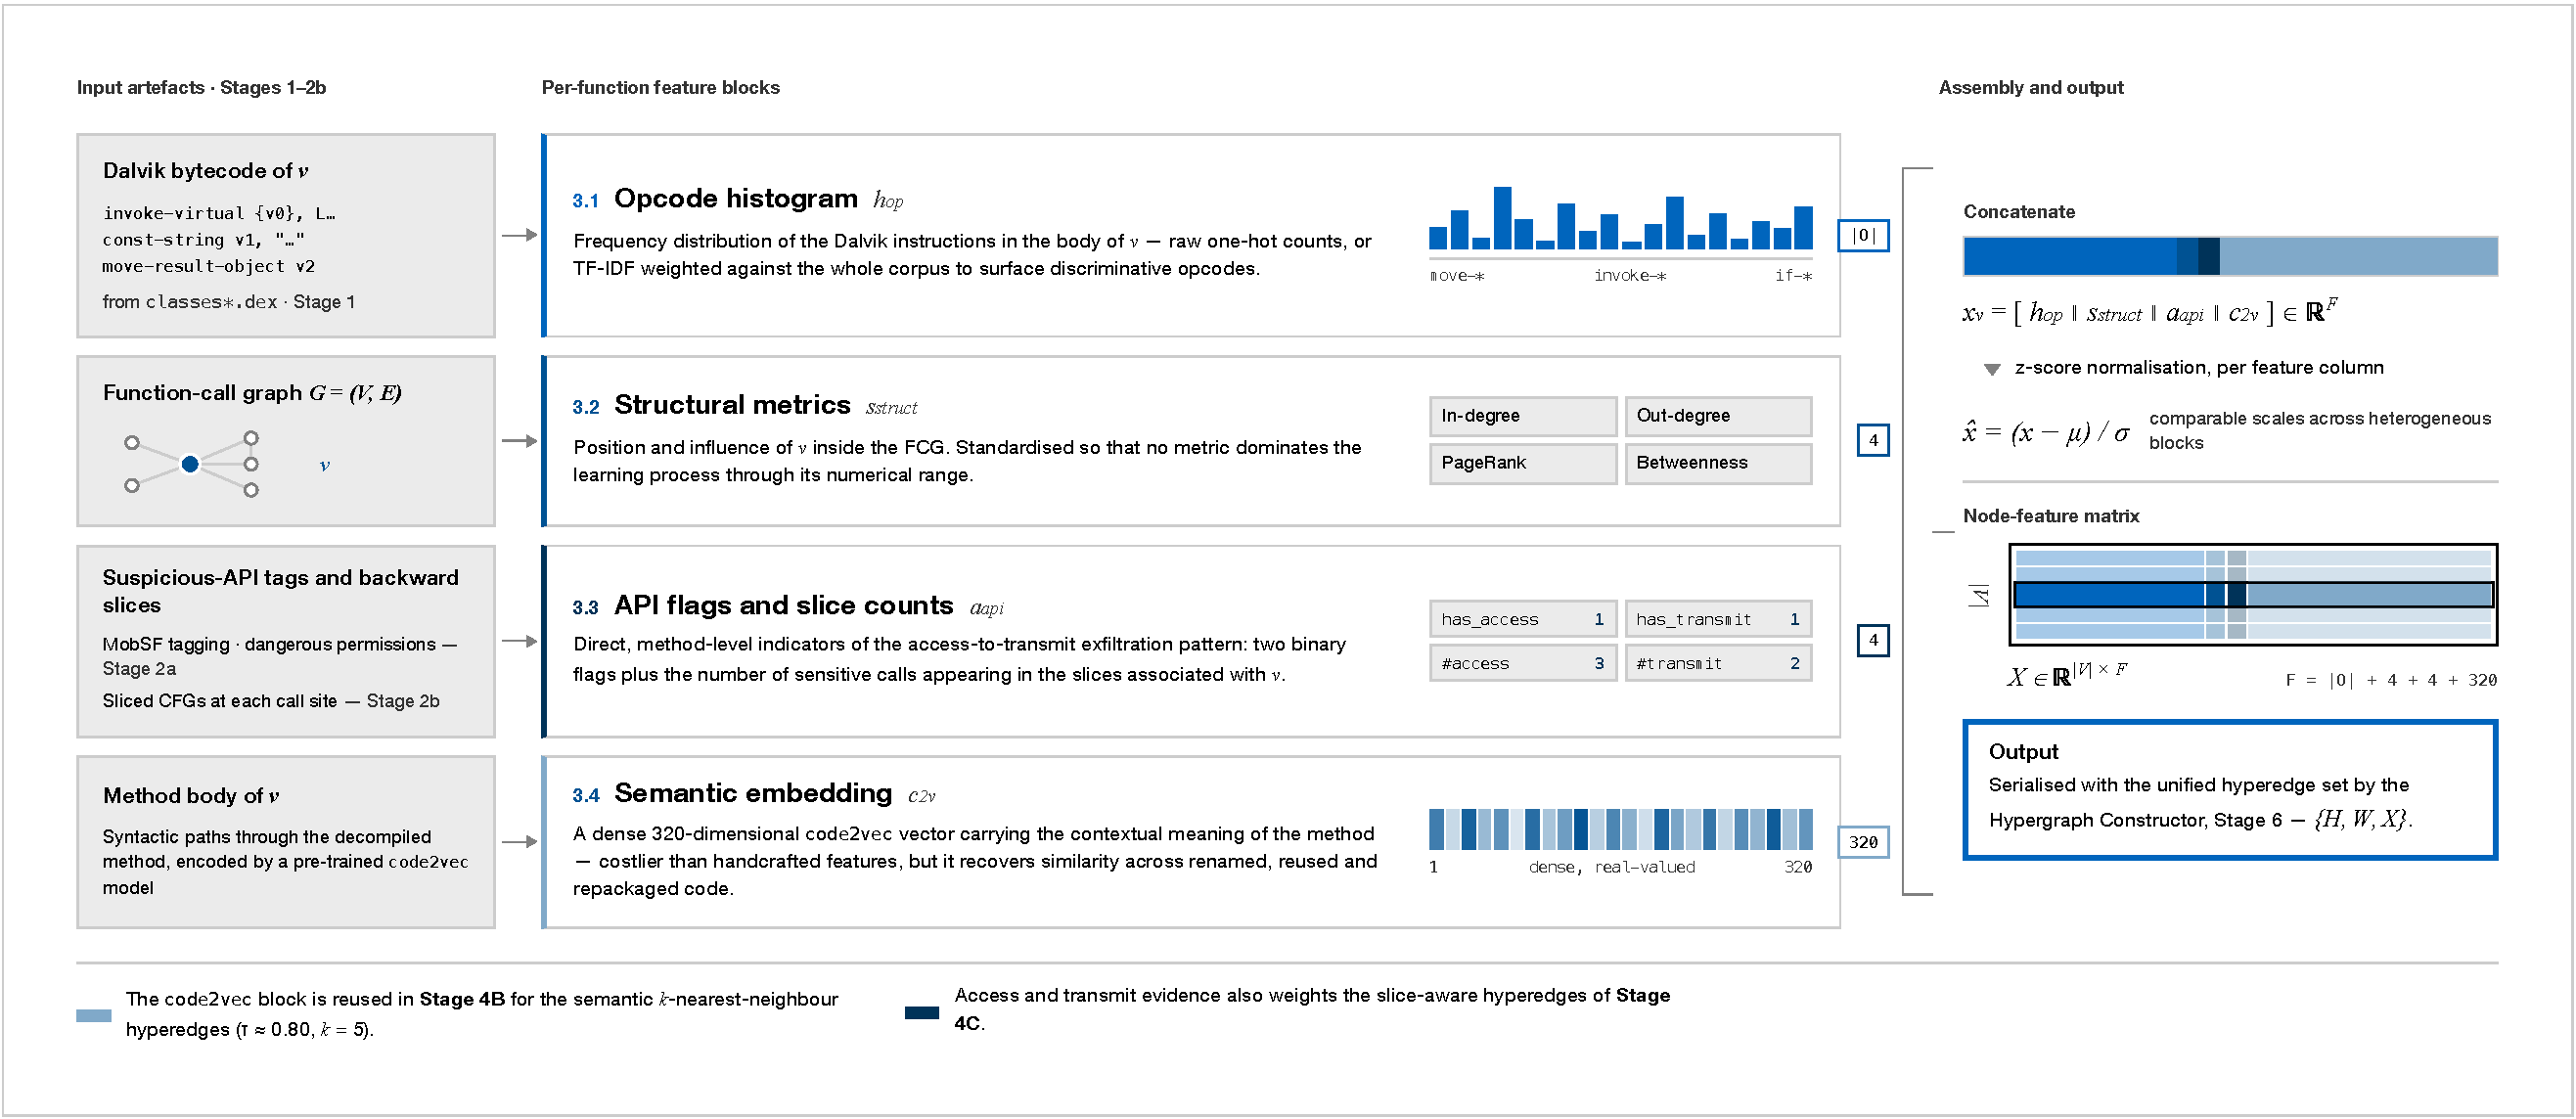
\includegraphics[width=\textheight]{hgann-mal/hgann-mal-node-features.pdf}
  \caption[Construction of the node feature vector in Stage 3]{Construction of the node feature
  vector in Stage~3. For each method $v$ of the function-call graph, an opcode histogram, four
  structural centrality metrics, four suspicious-API flags and counts, and a 320-dimensional
  code2vec embedding are computed from the artefacts of Stages~1 to~2b. The four blocks are
  concatenated into $x_v$ and z-score normalised, which yields the node-feature matrix
  $X \in \mathbb{R}^{\lvert V \rvert \times F}$ consumed by the hypergraph constructor in
  Stage~6.}
  \label{fig:hgann:node-features}
\end{sidewaysfigure}

\begin{table}
  \caption{The four groups of node feature. The width of the first group is the size of the
  opcode vocabulary.}
  \label{tab:hgann:features}
  \centering
  \begin{tabular}{llp{58mm}}
    \toprule
    Group & Width & What it records \\
    \midrule
    Opcode histogram   & vocabulary   & the distribution of Dalvik instructions in the method body \\
    Structural metrics & 4            & in-degree, out-degree, PageRank and betweenness centrality of the method in $G$ \\
    API indicators     & 4            & whether the method reaches an access API and whether it reaches a transmission API, with the counts of each within the slices attached to it \\
    Semantic embedding & 320          & a code2vec representation of the decompiled method body \\
    \bottomrule
  \end{tabular}
\end{table}

The first group describes what a method does at instruction level, and it is the feature the
program-code branch of Chapter~\ref{chap:hybroid} also rests on, there as a learned embedding of
the opcode sequence rather than as a histogram. Operand values are not used, which removes the
constants and register numbers that vary between builds of the same code. The histogram can be
taken as raw counts or weighted by inverse document frequency across the corpus.

The second group places the method in the call graph rather than describing its body, and it is
the only group that changes when the graph changes. The third connects the vertex to the analysis
of Section~\ref{sec:hgann:5}, so that a method reaching a sensitive API is distinguishable before
any hyperedge is built. Both are small, and together they contribute eight of the dimensions.

The fourth group is the largest. code2vec represents a method as a bag of paths through its
abstract syntax tree and learns a fixed-width vector from that bag \cite{alon2019code2vec}. The
published method consumes Java source, and the released model was trained on a corpus of Java
source, whereas the input here is Dalvik bytecode recovered from a distributed package. The
candidate confirms that the two were bridged by decompilation: each method was decompiled to Java
with DAD, the decompiler built into Androguard, and embedded with a ready-made, pre-trained
code2vec model. The source publication records neither step, and the width it reports differs
from the released model's.

The embedding of a method therefore depends on how completely the decompiler recovers its source,
as well as on the model. That dependence matters for the construction too. The semantic hyperedges
of Section~\ref{sec:hgann:7} are built from cosine similarities between these embeddings, so the
decompiler and the model shape one of the three construction rules as well.

\section{Hyperedge Construction}
\label{sec:hgann:7}

The lifting from a graph to a hypergraph is where the representation is decided. Stages 4A to 4C
apply three rules of different kinds to the same vertex set, and Stages 5 and 6 merge and assemble
what they produce. Write $\mathcal{H} = (\mathcal{V}, \mathcal{E}, w)$ for the result, with
$\mathcal{V} = V$ the methods of the call graph. Figure~\ref{fig:hgann:hyperedge-generation} draws
one hyperedge of each kind together with the parameters of its rule. Its panels keep the names
$H_{\mathrm{K}}$, $H_{\mathrm{SEM}}$ and $H_{\mathrm{API}}$ that the source gives the three lists,
which Equation~\ref{eq:hgann:merge} writes as the candidate sets $\mathcal{C}_{\text{topo}}$,
$\mathcal{C}_{\text{sem}}$ and $\mathcal{C}_{\text{sus}}$.

\begin{sidewaysfigure}
  \centering
  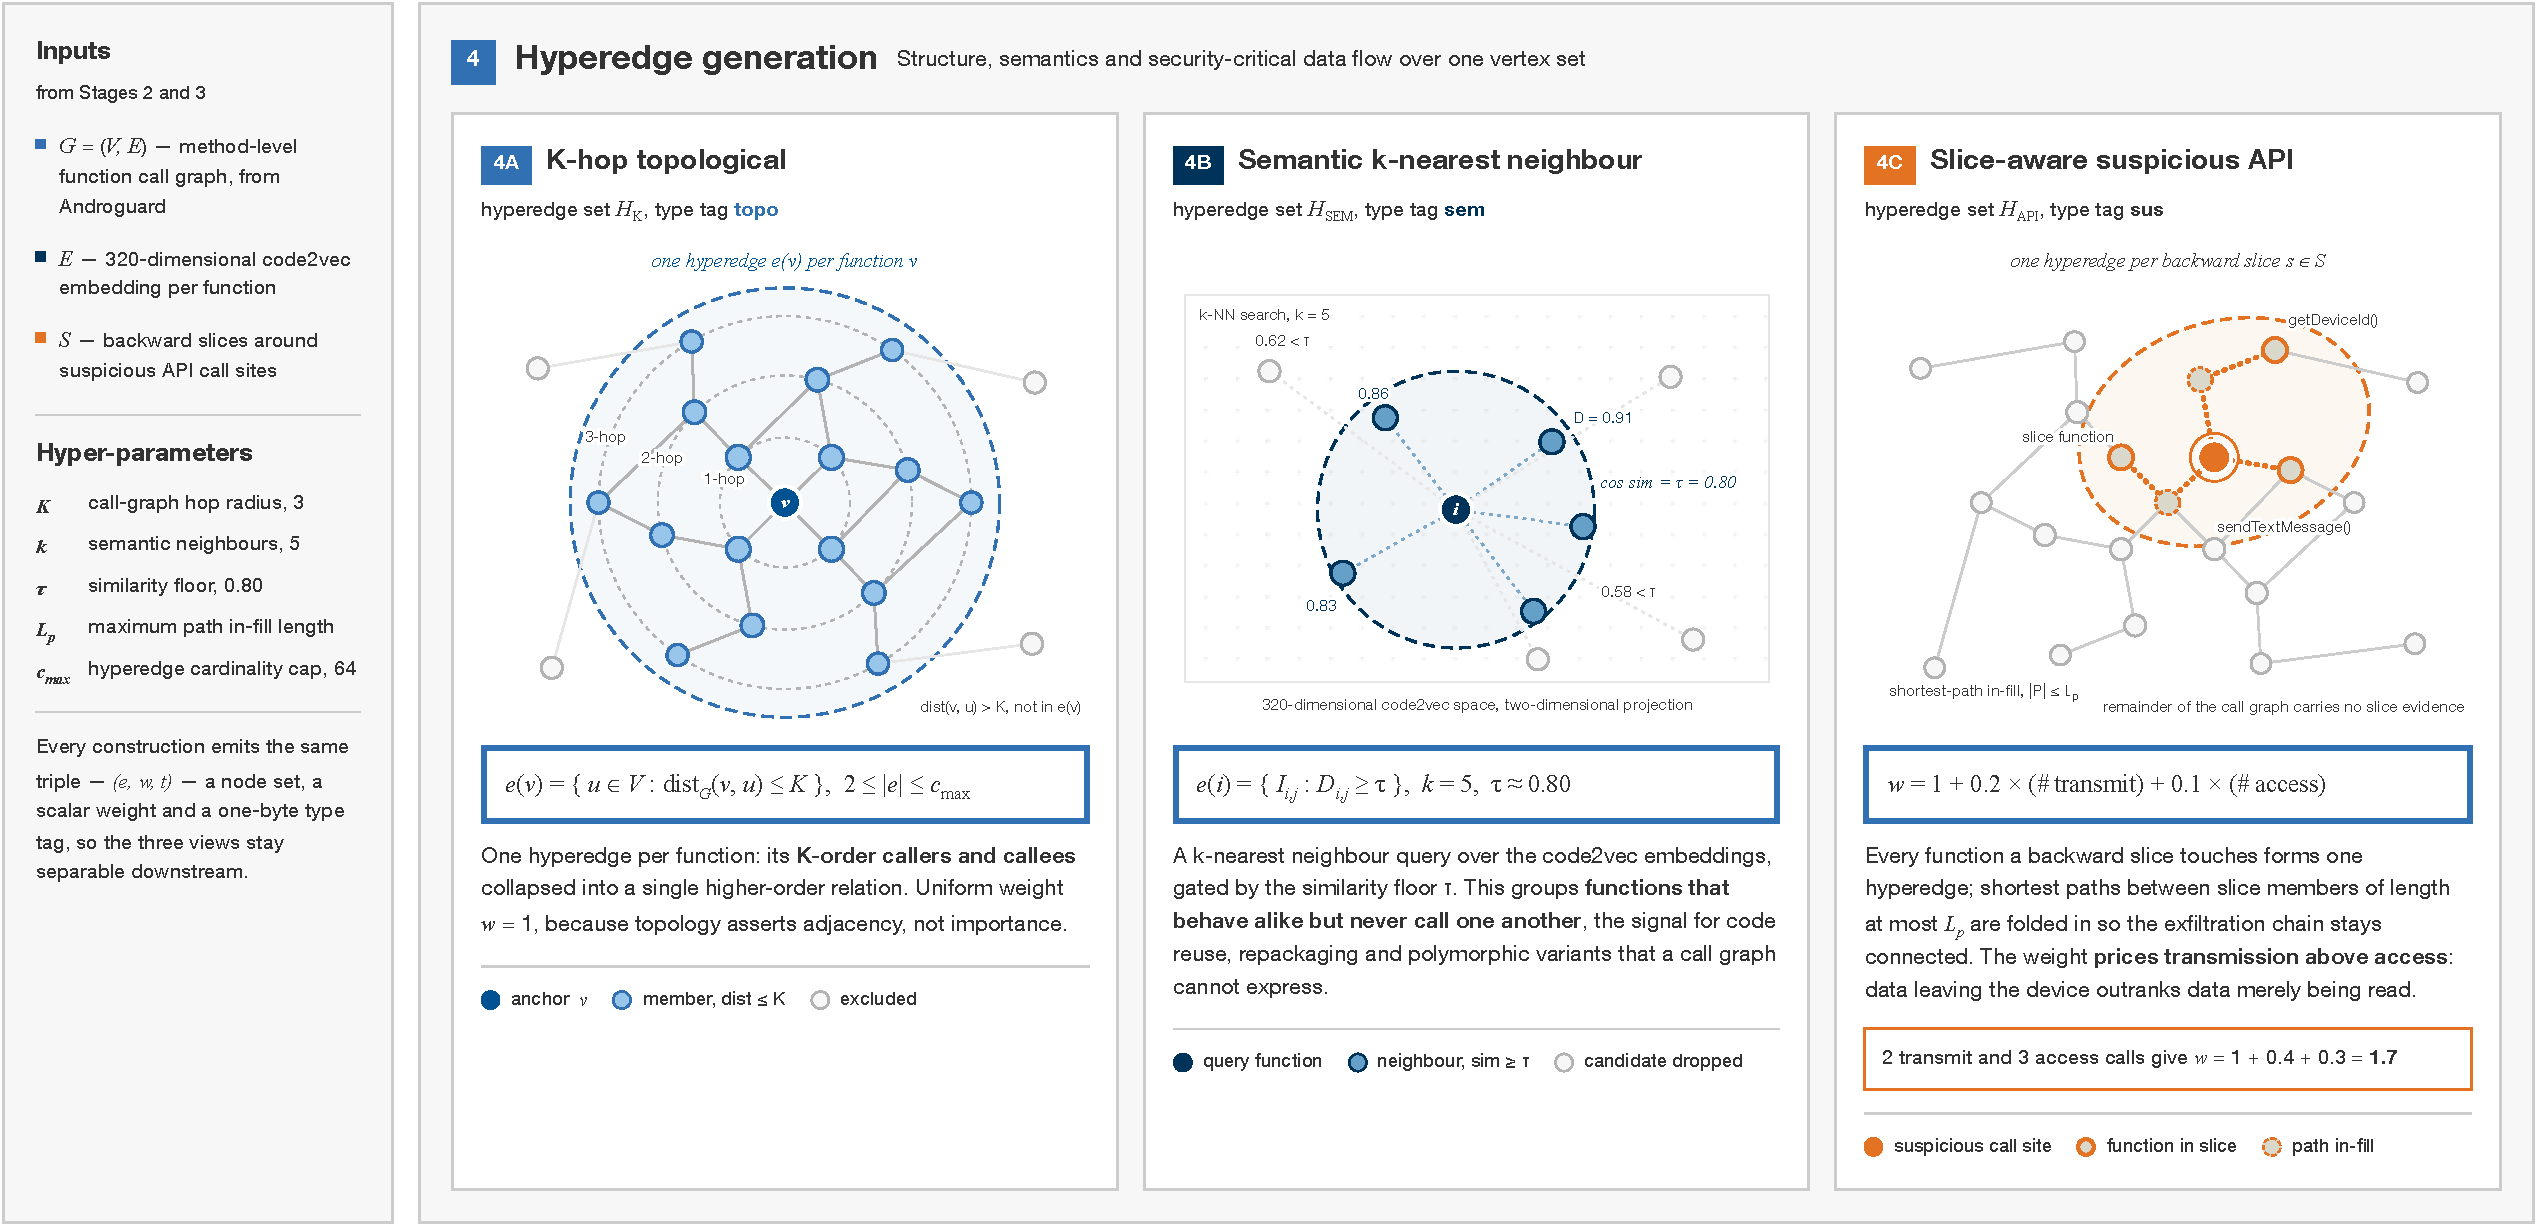
\includegraphics[width=\textheight]{hgann-mal/hgann-mal-hyperedge-generation.pdf}
  \caption[Hyperedge generation in Stage 4]{Hyperedge generation in Stage~4: three complementary
  constructions over one vertex set of methods. (4A)~Topological hyperedges take the $K$-hop ball
  around every method in the call graph, with $K = 3$ and uniform weight $w = 1$. (4B)~Semantic
  hyperedges are $k$-nearest-neighbour groups in the 320-dimensional code2vec space, with $k = 5$,
  admitted only above the similarity floor $\tau \approx 0.80$. (4C)~Slice-aware hyperedges are
  built from the backward slices of Stage~2b, extended with shortest paths of length at most $L_p$
  between slice members, and weighted $w = 1 + 0.2\,\#\text{transmit} + 0.1\,\#\text{access}$.
  A candidate with fewer than 2 or more than 64 members is rejected. Node colour marks hyperedge
  membership only.}
  \label{fig:hgann:hyperedge-generation}
\end{sidewaysfigure}

\paragraph{Topological hyperedges.} The source collects, for each method $v$, its callers and
callees up to order $K$. Let $\vec{d}_G(v,u)$ be the number of call edges on a shortest directed
path from $v$ to $u$, with $\vec{d}_G(v,u) = \infty$ when there is none, and let
$\operatorname{dist}_G(v,u) = \min\{\vec{d}_G(v,u), \vec{d}_G(u,v)\}$. Then
\begin{equation}
  e_{\text{topo}}(v) = \{\, u \in V : \operatorname{dist}_G(v, u) \le K \,\}, \qquad K = 3 ,
  \label{eq:hgann:topo}
\end{equation}
holds $v$ together with its callers and callees up to $K$ steps away. This convention follows the
wording of the source. A distance measured with call directions ignored would also admit the other
callees of a caller and would give larger hyperedges, and the source does not record which
convention the implementation used.
This is the rule the earlier hypergraph work on Android uses, there in combination with a
permission-based rule \cite{zhang2023android}. It records a neighbourhood as one object rather
than as a set of pairs, which is the whole of the higher-order claim at this point: a vertex and
its $K$-hop neighbourhood enter the operator together.

\paragraph{Semantic hyperedges.} A nearest-neighbour search over the code2vec embeddings, computed
with the FAISS library, groups methods whose representations are close. Write
$c_v \in \mathbb{R}^{320}$ for the embedding of method $v$, the fourth group of
Table~\ref{tab:hgann:features}; the full feature vector $x_v$ also carries the other three groups,
and the search uses the embedding alone. The candidate confirms that the search compares cosine
similarities, $\operatorname{sim}(a, b) = a^{\top} b / (\lVert a \rVert\, \lVert b \rVert)$, and
that it runs within one application. With $\mathcal{N}_k(v)$ the $k$ methods of the same
application, other than $v$, that score highest under $\operatorname{sim}$,
\begin{equation}
  e_{\text{sem}}(v) = \{v\} \cup \{\, u \in \mathcal{N}_k(v) : \operatorname{sim}(c_v, c_u) \ge \tau \,\},
  \qquad k = 5, \quad \tau \approx 0.80 .
  \label{eq:hgann:sem}
\end{equation}
The original algorithm, whose test panel~4B of Figure~\ref{fig:hgann:hyperedge-generation}
reproduces, names the search output $D$, a letter that suggests a distance, and keeps a neighbour
when $D \ge \tau$. The test agrees with the cosine similarity, since for a distance the inequality
would run the other way. The query
method is included and is not counted among its $k$ neighbours, so
$\lvert e_{\text{sem}}(v) \rvert \le k + 1$; the source does not say whether its search counted the
query itself. Nothing in this rule refers to the call graph, which is the point of including it:
two methods that never call one another, and that sit in different parts of the application, are
joined when they do the same kind of work. The source names polymorphic malware and code reuse as
the intended cases. Because the search stays inside one application, a semantic hyperedge joins
methods of that application only, and code shared across a family can make the hyperedges of
different applications alike without joining them.

\paragraph{Slice-aware hyperedges.} Each backward slice $s$ from Section~\ref{sec:hgann:5} yields
one hyperedge over the methods the slice contains, extended by the methods on short call paths
between them. Let $F_s$ be that member set, fixed before any path is added. For a directed path $P$
in the call graph, let $V(P)$ be its methods and $\ell(P)$ its number of call edges, and let
$P_{uv}$ be a shortest path from $u$ to $v$. Then
\begin{equation}
  e_{\text{sus}}(s) = F_s \;\cup
  \bigcup_{\substack{u, v \in F_s,\ u \ne v\\ P_{uv} \text{ exists},\ \ell(P_{uv}) \le L_p}}
  V(P_{uv}) .
  \label{eq:hgann:sus}
\end{equation}
Only pairs of original members are joined, so a method that one path adds does not start further
paths. The original algorithm loops over the pairs of the set it is enlarging, and freezing $F_s$ is
the convention adopted here to make the result independent of the loop order. A pair with no
directed path contributes nothing. Where several shortest paths exist, the one chosen decides which
methods join. This family carries the only non-unit weight in the hypergraph:
\begin{equation}
  w(e_{\text{sus}}(s)) = 1 + 0.2\,\#\text{transmit}(s) + 0.1\,\#\text{access}(s) ,
  \label{eq:hgann:weight}
\end{equation}
so a slice that both reads private data and sends it weighs more than one that only reads, and the
transmission end weighs twice the access end. The weight is a construction heuristic, so it cannot
be read as a probability of exfiltration.

\paragraph{Merging.} Each rule proposes candidate triples $(e, w, t)$ of a member set, a weight and
a type tag. Collected as a multiset and passed through the post-processing of the source, they give
\begin{equation}
  \mathcal{C} = \mathcal{C}_{\text{topo}} \uplus \mathcal{C}_{\text{sem}} \uplus \mathcal{C}_{\text{sus}} ,
  \qquad
  \mathcal{E} = \operatorname{Post}_{\eta}\bigl( \{\, (e, w, t) \in \mathcal{C} :
  2 \le \lvert e \rvert \le c_{\max} \,\} \bigr) ,
  \qquad c_{\max} = 64 .
  \label{eq:hgann:merge}
\end{equation}
The lower bound removes singletons, which carry no relation, and with them every slice that has a
single member, since such a slice has no pair to join. The upper bound is described in the source
publication as necessary for stable message passing. Its prose says that hyperedges are capped,
whereas its algorithm rejects a candidate outside the interval. This chapter follows the algorithm:
truncation would need a rule for choosing which members to keep, and none is given. Rejection has a
consequence of its own. A method whose $K$-step neighbourhood holds more than 64 methods loses its
topological hyperedge entirely, so the topological family omits exactly the methods with the
largest neighbourhoods.

The operator $\operatorname{Post}_{\eta}$ removes duplicates. Two candidates with the same members
can carry different weights or tags, as a slice hyperedge and a topological one over the same
methods would, and the policy $\eta$ that decides which weight and which tag survive is not
recorded; this chapter does not supply one. Filtering can also leave a method in no hyperedge, for
instance an isolated method that belongs to no slice and has no semantic neighbour above $\tau$.
Its degree is then zero and the normalisation of Section~\ref{sec:hgann:8} is undefined for it, and
the source does not say whether such methods were dropped or handled in another way.

Each surviving hyperedge is tagged with its family in one byte, and the incidence matrix $H$ and
the diagonal weight matrix $W$ are assembled from the result and serialised per application.
Algorithm~\ref{alg:hgann:construction} restores the construction procedure of the source
publication with the conventions above written into it. It also adds the post-processing and the
sparse assembly, which the output line of the original announces and its body omits. The type tag
records something the operator never reads. The layer described in
Section~\ref{sec:hgann:8} consumes $H$, $W$ and $X$, so a hyperedge's family influences the model
only through its weight, and since two of the three families carry weight one, the topological and
semantic hyperedges are indistinguishable to the operator once they are built. That is a design
gap rather than an error, and Section~\ref{sec:hgann:13} names it as the cleanest available
extension.

\begin{algorithm}[tbp]
  \caption[Construction and assembly of the \hgann{} hypergraph]{Construction and assembly of the
  \hgann{} hypergraph. Stages 4A to 4C restore the algorithm of the source publication
  \cite{norouzian2025hgannmal} with the conventions of Equations~\ref{eq:hgann:topo}
  to~\ref{eq:hgann:sus} written in; stages 5 and 6 add the post-processing and assembly that its
  prose describes.}
  \label{alg:hgann:construction}
  \small
  \textbf{Input:} call graph $G = (V, E)$; embeddings $c_v$; slices $s \in \mathcal{S}$ with
  member sets $F_s$; parameters $K$, $k$, $\tau$, $L_p$, $c_{\max}$; duplicate policy $\eta$\par
  \textbf{Output:} sparse incidence matrix $H$, weight matrix $W$, type tags $t$
  \begin{algorithmic}[1]
    \Statex \textbf{Stage 4A: topological hyperedges}
    \State $\mathcal{C} \gets \varnothing$ \Comment{multiset of candidates}
    \For{$v \in V$}
      \State $e \gets \{u \in V : \operatorname{dist}_G(v,u) \le K\}$
      \If{$2 \le \lvert e \rvert \le c_{\max}$}
        \State $\mathcal{C} \gets \mathcal{C} \uplus \{(e, 1, \texttt{topo})\}$
      \EndIf
    \EndFor
    \Statex \textbf{Stage 4B: semantic ($k$-NN) hyperedges}
    \State $(I, S) \gets \textsc{Faiss}(\{c_v\}_{v \in V}, k)$
      \Comment{$k$ others per method; $S$ holds cosine similarities}
    \For{$v \in V$}
      \State $e \gets \{v\} \cup \{I_{v,j} : S_{v,j} \ge \tau\}$
      \If{$2 \le \lvert e \rvert \le c_{\max}$}
        \State $\mathcal{C} \gets \mathcal{C} \uplus \{(e, 1, \texttt{sem})\}$
      \EndIf
    \EndFor
    \Statex \textbf{Stage 4C: slice-aware hyperedges}
    \For{$s \in \mathcal{S}$}
      \State $e \gets F_s$; \ $w \gets 1 + 0.2\,\#\text{transmit}(s) + 0.1\,\#\text{access}(s)$
      \For{$(u, v) \in F_s \times F_s$ with $u \ne v$} \Comment{$F_s$ is not enlarged}
        \If{$P_{uv}$ exists and $\ell(P_{uv}) \le L_p$}
          \State $e \gets e \cup V(P_{uv})$
        \EndIf
      \EndFor
      \If{$2 \le \lvert e \rvert \le c_{\max}$}
        \State $\mathcal{C} \gets \mathcal{C} \uplus \{(e, w, \texttt{sus})\}$
      \EndIf
    \EndFor
    \Statex \textbf{Stage 5: post-processing}
    \State $\mathcal{E} \gets \operatorname{Post}_{\eta}(\mathcal{C})$
      \Comment{policy $\eta$ not recorded}
    \Statex \textbf{Stage 6: sparse assembly}
    \For{$j = 1, \ldots, \lvert \mathcal{E} \rvert$, with $(e_j, w_j, t_j)$ the $j$-th element
      of $\mathcal{E}$}
      \State $H_{vj} \gets 1$ for every $v \in e_j$; \ $W_{jj} \gets w_j$; \ $t(j) \gets t_j$
    \EndFor
    \State \Return $H$, $W$, $t$
  \end{algorithmic}
\end{algorithm}

\section{Hypergraph Attention Model}
\label{sec:hgann:8}

The operator is defined over the structure fixed in
Section~\ref{sec:background:graphs:hypergraphs}, whose notation is used here without restatement:
the incidence matrix $H$, the weighted vertex degree $d(v)$ and the hyperedge degree $\delta(e)$
with their diagonal matrices $D_v$ and $D_e$, and the diagonal weight matrix $W$. Write
$n = \lvert \mathcal{V} \rvert$, and assume for now that $d(v) > 0$ for every method;
Section~\ref{sec:hgann:7} records that filtering can violate this. The hypergraph Laplacian is
\begin{equation}
  L = I - P_0 , \qquad P_0 = D_v^{-1/2} H W D_e^{-1} H^{\top} D_v^{-1/2} ,
  \label{eq:hgann:laplacian}
\end{equation}
and for a signal $f \in \mathbb{R}^{n}$ over the methods it has the energy
\begin{equation}
  f^{\top} L f = \frac{1}{2} \sum_{e \in \mathcal{E}} \frac{w(e)}{\delta(e)}
  \sum_{u, v \in e} \left( \frac{f_u}{\sqrt{d(u)}} - \frac{f_v}{\sqrt{d(v)}} \right)^{2} ,
  \label{eq:hgann:energy}
\end{equation}
where the inner sum runs over ordered pairs \cite{zhou2006learning}. The energy is small when the
degree-normalised signal varies little inside the constructed groups, and each hyperedge counts in
proportion to its weight and in inverse proportion to its size. It describes the operator and is
not a term of the training loss. One layer of hypergraph convolution propagates through $P_0$:
\begin{equation}
  X^{(l+1)} = \sigma\!\left( D_v^{-1/2} H W D_e^{-1} H^{\top} D_v^{-1/2} X^{(l)} \Theta^{(l)} \right) ,
  \label{eq:hgann:conv}
\end{equation}
with $\Theta^{(l)}$ the learned projection of layer $l$ and $\sigma$ a non-linearity. Read from
right to left, the operator gathers vertex states into the hyperedges that contain them, averages
within each hyperedge through $D_e^{-1}$, scales by the hyperedge weight, and returns the result to
the member vertices with the symmetric normalisation of $D_v^{-1/2}$. One layer therefore couples
every pair of methods that share a hyperedge. The matrix $P_0$ is positive semidefinite and similar
to the row-stochastic matrix $D_v^{-1} H W D_e^{-1} H^{\top}$, so its eigenvalues lie in $[0,1]$.
Equation~\ref{eq:hgann:conv} thus multiplies each eigencomponent of $L$ with eigenvalue $\lambda$ by
$1 - \lambda$, and the components with the highest energy are damped most. This is the smoothing
behind the low-pass bias recorded in Section~\ref{sec:background:learning:hypergraphconvolution}.

\subsection*{Attention over hyperedges}

Equation~\ref{eq:hgann:conv} weights a vertex's hyperedges by $W$, which is fixed when the
hypergraph is built. Attention replaces the binary membership indicator by a learned real value,
so that the strength with which a vertex participates in a hyperedge is trained
\cite{bai2021hypergraphattention}. The layer index is dropped from here on. Let
$X \in \mathbb{R}^{n \times F}$ hold the input states as rows, let
$\Theta \in \mathbb{R}^{F \times F'}$ be the projection, and set $Y = X\Theta$, with
$y_v \in \mathbb{R}^{F'}$ the row of method $v$ read as a column vector. A hyperedge is first
represented by the mean of the projected states of its members,
\begin{equation}
  z_e = \frac{1}{\delta(e)} \sum_{u \in e} y_u ,
  \label{eq:hgann:hedgerep}
\end{equation}
and the coefficient joining a vertex to one of its hyperedges is the normalised score
\begin{equation}
  \alpha(v, e) = \frac{\exp\bigl( \sigma( a^{\top} [\, y_v \,\Vert\, z_e \,] ) \bigr)}
                      {\sum_{e' \ni v} \exp\bigl( \sigma( a^{\top} [\, y_v \,\Vert\, z_{e'} \,] ) \bigr)} ,
  \label{eq:hgann:attn}
\end{equation}
with $a \in \mathbb{R}^{2F'}$ a learned vector and $\Vert$ concatenation. Collecting the
coefficients into $H_{\text{att}}$, whose entry at $(v,e)$ is $\alpha(v,e)$ where $H$ has a one and
zero elsewhere, gives the layer actually used:
\begin{equation}
  X' = \sigma\!\left( D_v^{-1/2} H_{\text{att}} W D_e^{-1} H_{\text{att}}^{\top} D_v^{-1/2}
              X \Theta \right) .
  \label{eq:hgann:attnprop}
\end{equation}
The degree matrices are those of the binary $H$, as in the source publication; degrees recomputed
from $H_{\text{att}}$ would define a different layer. Gradients reach $H_{\text{att}}$ as well as
$X$ and $\Theta$, so the membership weights are learned. The support is not. $H_{ve} = 0$ implies
$\alpha(v,e) = 0$, and a finite score gives every present membership a positive coefficient, so
training reweights the memberships the construction produced and cannot add a method to a
hyperedge or remove one.

Equations~\ref{eq:hgann:hedgerep} and~\ref{eq:hgann:attn} state the additive form of the score,
which the source publication leaves as an uninstantiated similarity function and which the
candidate confirms is what was implemented. The published formulation also writes the score
between two vertices while indexing it by a hyperedge; the form above resolves that by scoring a
vertex against a representation of the hyperedge, which is what the implementation computes.

\subsection*{The messages between methods}

Expanding Equation~\ref{eq:hgann:attnprop} shows what one method receives from another. The layer
runs in two stages. Each hyperedge first forms a message, and each method then combines the
messages of its hyperedges:
\begin{equation}
  \mu_e = \frac{1}{\delta(e)} \sum_{u \in e} \frac{\alpha(u,e)}{\sqrt{d(u)}}\, y_u ,
  \qquad
  x'_v = \sigma\biggl( \frac{1}{\sqrt{d(v)}} \sum_{e \ni v} w(e)\, \alpha(v,e)\, \mu_e \biggr) .
  \label{eq:hgann:messages}
\end{equation}
Substituting the first expression into the second gives one matrix of couplings between methods,
\begin{equation}
  X' = \sigma\bigl( P_{\text{att}} X \Theta \bigr) ,
  \qquad
  P_{\text{att}}(v,u) = \frac{1}{\sqrt{d(v)\, d(u)}} \sum_{e \ni v,u} \frac{w(e)}{\delta(e)}\,
  \alpha(v,e)\, \alpha(u,e) .
  \label{eq:hgann:coupling}
\end{equation}
Two methods interact only through the hyperedges they share, and each shared hyperedge adds one
term. In that term the coefficient of the sender and the coefficient of the receiver appear as a
product. The construction weight $w(e)$ is a separate factor, so the slice heuristic of
Equation~\ref{eq:hgann:weight} and the learned coefficients act on a message independently. The
coefficients depend on the layer input through Equations~\ref{eq:hgann:hedgerep}
and~\ref{eq:hgann:attn}, which makes $P_{\text{att}}$ a function of $X$; for a fixed input it is a
symmetric matrix.

The key $z_e$ and the message $\mu_e$ are different aggregations over the same members. The key is
an unweighted mean, whereas the message weights each member $u$ by $\alpha(u,e) / \sqrt{d(u)}$, so
attention changes the average inside a hyperedge as well as the weighting across the hyperedges of
a method. It does not change the sign of any term. Every member enters $\mu_e$ with a positive
coefficient, so before the non-linearity each output is the projection of a non-negative
combination of input states, and one layer cannot form a difference between two members of a
hyperedge. The high-frequency component that standard hypergraph convolution discards has been
characterised \cite{li2026highpass}. Attention changes the proportions of that average and keeps
every coefficient positive, so the propagation of one layer remains an averaging of member states.

Grouping the sum in Equation~\ref{eq:hgann:coupling} by hyperedge gives a structural statement:
\begin{equation}
  P_{\text{att}} = \sum_{e \in \mathcal{E}} \frac{w(e)}{\delta(e)}\, \psi_e \psi_e^{\top} ,
  \qquad
  (\psi_e)_v = \frac{\alpha(v,e)}{\sqrt{d(v)}} ,
  \label{eq:hgann:rankone}
\end{equation}
with $\alpha(v,e) = 0$ for $v \notin e$. Each hyperedge adds a positive semidefinite matrix of rank
one, and because every weight is positive, $P_{\text{att}}$ is positive semidefinite for every
input. The statement concerns the propagation matrix at a fixed input. It carries no guarantee about
the convergence of training.

Because $\alpha(v,e)$ depends on both the method and its hyperedge, two different hyperedge
groupings can produce the same fixed matrix $P_0$ yet different attentive propagation matrices.
The reported experiments do not determine whether the learned model used this capacity or whether
it caused the measured accuracy differences.

\subsection*{What the mechanism can and cannot be claimed to do}

Two further properties bound what the chapter claims for the operator.

The first concerns the ranking that the score induces. Splitting $a = (a_1, a_2)$ across the
concatenation writes the argument of $\sigma$ in Equation~\ref{eq:hgann:attn} as $q_v + b_e$, with
a query term and a hyperedge key
\begin{equation}
  q_v = a_1^{\top} y_v , \qquad b_e = a_2^{\top} z_e .
  \label{eq:hgann:split}
\end{equation}
If $\sigma$ is strictly increasing, then for a fixed layer input and any two hyperedges $e_1$ and
$e_2$ that contain $v$,
\begin{equation}
  \alpha(v, e_1) > \alpha(v, e_2) \iff b_{e_1} > b_{e_2} .
  \label{eq:hgann:ranking}
\end{equation}
The proof is short. Because $\sigma$ and $\exp$ are strictly increasing, the numerators of
Equation~\ref{eq:hgann:attn} are ordered as the keys are, and the two coefficients share one
positive denominator. Any two methods therefore rank the hyperedges they share in the same order,
and the keys alone fix that order. Methods can still attend to different hyperedges, since each
normalises over its own. A non-decreasing activation such as ReLU can merge two hyperedges into a
tie but cannot reverse their order between methods. The argument is the one Brody et al.\ give for
the additive score of pairwise graph attention \cite{brody2022gatv2}, applied to the score of
Equation~\ref{eq:hgann:attn}. It holds for each attention head separately and says nothing about
hypergraph attention with other scoring functions. Under either kind of activation, the restriction
on wording that the chapter keeps is thus a result for this operator: within one layer, \hgann{}
can learn which hyperedges matter, and it cannot reverse their order from one method to another.

The query term does not cancel, however. With $\sigma$ a leaky ReLU of slope 0.2 and keys $-1$
and $1$, the coefficients are approximately $0.23$ and $0.77$ for $q_v = 0$, and $0.12$ and $0.88$
for $q_v = 2$. The order agrees and the values differ. Cancellation is exact when $\sigma$ is affine
on the arguments of one method, as a leaky ReLU is when they share a sign.

The second concerns normalisation. Uniform coefficients do not reproduce
Equation~\ref{eq:hgann:conv}, because the degrees in Equation~\ref{eq:hgann:attnprop} are those of
the binary $H$. Let $r_v$ be the number of hyperedges containing $v$ and
$R = \operatorname{diag}(r_v)$. Equal scores give $H_{\text{att}} = R^{-1} H$ and hence
\begin{equation}
  P_{\text{att}} = R^{-1} P_0 R^{-1} ,
  \label{eq:hgann:uniform}
\end{equation}
which reduces to $P_0 / r^2$ when every method lies in $r$ hyperedges, and to $P_0 / 4$ in the
example above. An ablation that replaced the learned coefficients by uniform ones would therefore
change the scale of propagation as well as its weighting. A comparison with the non-attentive
operator needs a stated normalisation convention before a difference can be read as an effect of
attention.

\subsection*{Read-out and classification}

Applications differ in size, so the vertex states are collapsed into one vector per application.
Two variants are named in the source publication, an unweighted mean over the vertices and a
learned attention pooling.

Training and inference run on batches. The source assembles a batch of $B$ applications by placing
their incidence and weight matrices on a block diagonal and stacking their feature matrices,
\begin{equation}
  H_{\mathcal{B}} = \operatorname{diag}(H_1, \ldots, H_B) , \qquad
  W_{\mathcal{B}} = \operatorname{diag}(W_1, \ldots, W_B) , \qquad
  X_{\mathcal{B}} = \begin{bmatrix} X_1 \\ \vdots \\ X_B \end{bmatrix} ,
  \label{eq:hgann:batch}
\end{equation}
together with an index that maps each row of $X_{\mathcal{B}}$ to its application. No hyperedge
spans two blocks, so degrees, keys, coefficients and messages are all computed inside one
application. The output for an application therefore does not depend on the other applications in
its batch, and the read-out uses the index to pool each block on its own.

The layer is also equivariant under relabelling. Let $\Pi$ reorder the methods of an application
and $Q$ its hyperedges, and write $\Phi(X, H, W)$ for the output of
Equation~\ref{eq:hgann:attnprop}. Then
\begin{equation}
  \Phi(\Pi X, \Pi H Q^{\top}, Q W Q^{\top}) = \Pi\, \Phi(X, H, W) , \qquad
  g(\Pi X, \Pi H Q^{\top}, Q W Q^{\top}) = g(X, H, W) ,
  \label{eq:hgann:invariance}
\end{equation}
where $g$ is the application vector. The first identity holds because the degree matrices, the keys
and the coefficients all permute with $H$, and the second because both read-outs are symmetric in
the vertex states. The prediction therefore does not depend on the order in which method rows or
hyperedge columns are stored. This concerns the hypergraph once it is built. It gives no resistance
to obfuscation, and order-dependent choices earlier in the pipeline, such as tie-breaking among
nearest neighbours or among shortest paths, can change $H$ itself.

That vector passes through a shared multi-layer perceptron with two hidden layers, rectified
linear activations and dropout, and then into two heads. The first emits a single logit whose
sigmoid is the probability that the application is malicious. The second emits one logit per class
of the labelled taxonomy, normalised by a softmax. Training minimises the sum of the two
objectives,
\begin{equation}
  \mathcal{L} = \lambda_{\text{bin}} \operatorname{BCE}(z_{\text{bin}}, y_{\text{bin}})
              + \lambda_{\text{fam}} \operatorname{CE}(z_{\text{fam}}, y_{\text{fam}}) ,
  \label{eq:hgann:loss}
\end{equation}
weighted by two constants.

Equation~\ref{eq:hgann:loss} applies both terms unconditionally. On the corpus of
Section~\ref{sec:hgann:12}, benign
applications form one of the labelled classes and the second term is defined for them. On the
corpus of Section~\ref{sec:hgann:11} the classes are twenty malware families. A benign application
has no family among them, and neither has a malicious application from one of the smaller
families, so the family term has no target for either. One well-defined specification averages each
term over the training samples that carry its label,
\begin{equation}
  \mathcal{L} = \frac{\lambda_{\text{bin}}}{\lvert \mathcal{D}_{\text{bin}} \rvert}
  \sum_{i \in \mathcal{D}_{\text{bin}}} \operatorname{BCE}(z_{\text{bin},i}, y_{\text{bin},i})
  + \frac{\lambda_{\text{fam}}}{\lvert \mathcal{D}_{\text{fam}} \rvert}
  \sum_{i \in \mathcal{D}_{\text{fam}}} \operatorname{CE}(z_{\text{fam},i}, y_{\text{fam},i}) ,
  \label{eq:hgann:maskedloss}
\end{equation}
with $\mathcal{D}_{\text{bin}}$ and $\mathcal{D}_{\text{fam}}$ the non-empty sets of samples that
have a binary label and a class label.

\section{Datasets, Tasks, and Split Policy}
\label{sec:hgann:9}

Two corpora are used, and they answer to different needs. Drebin is the reference collection of
the field, which makes results on it comparable with a long line of published work, and its family
labels support a classification task that a category taxonomy cannot. CICMalDroid is newer, it
carries benign applications alongside malicious ones, and its labels are categories of behaviour
rather than families. Using both guards against a conclusion that holds only for one collection,
which is the reason the source publication gives for the second corpus.

\subsection*{Drebin}

Drebin is the malicious part of a larger collection gathered between August 2010 and October 2012
from the Google Play Store, from Chinese and Russian alternative markets, from Android websites and
malware forums, and from the whole of the Malgenome project \cite{arp2014drebin}. Every sample in
that collection was submitted to VirusTotal and judged by ten antivirus scanners; an application
was counted as malicious when at least two of the ten flagged it, applications labelled adware were
then removed, and 5,560 malicious samples remained. The family names are taken from the labels of
one of the ten scanners. The source publication of this chapter counts 179 families in the set
\cite{norouzian2025hgannmal}, a figure the dataset paper does not state. Family sizes are heavily
skewed, so the classification task uses the twenty largest, which cover 4,664 of the samples and
are drawn with their sizes in Figure~\ref{fig:hgann:class-distribution}(a). The 159 smaller
families hold the other 896 samples, 16.1 per cent of the set, and they are left out of the
family task only, since binary detection uses all 5,560 malicious samples.

\begin{figure}[tbp]
  \centering
  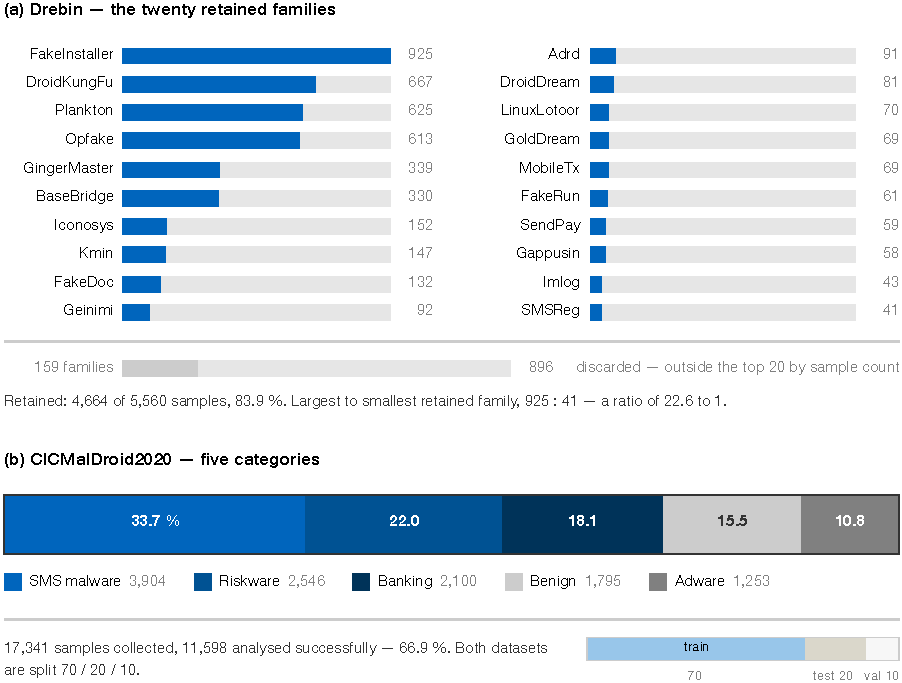
\includegraphics[width=\linewidth]{hgann-mal/hgann-mal-class-distribution.pdf}
  \caption[Class distribution of the two corpora]{Class distribution of the two corpora.
  (a)~The twenty largest Drebin families, the classes of the \familyclassification{} task. The
  159 smaller families, with 896 samples, take no part in that task and remain in binary
  detection. (b)~The five CICMalDroid 2020 categories of the published distribution
  \cite{mahdavifar2020dynamic}; Benign is the negative class of binary detection on this corpus.
  The long tail of Drebin is the reason the source publication reports an F1 score, which it
  labels Macro-F1, alongside accuracy.}
  \label{fig:hgann:class-distribution}
\end{figure}

Three properties of that construction bear on the results. The malicious label is a vote of two
scanners out of ten, which is a lower bar than a majority and admits samples the other eight
consider harmless. The ground truth for \familyclassification{} is one vendor's naming, which is a
convention rather than a taxonomy of behaviour. And the 123,453 benign packages the original
DREBIN work evaluated against are not part of what is distributed, which is why a negative class
had to be found elsewhere.

Binary detection needs a negative class, and Drebin supplies none, so the benign side was drawn at
random from AndroZoo \cite{allix2016androzoo}. AndroZoo collects Android applications by crawling
Google Play, the Chinese markets Anzhi and AppChina, and several smaller repositories; the crawl
began in late 2011 and has continued since, and the collection held more than three million
applications when it was first described. Every application in it has been submitted to
VirusTotal, and what the collection stores per application is the number of antivirus products
that flagged it, together with the compilation date of its bytecode, its size and the market it
came from.
About 9,470 benign applications were used against the full set of 5,560 malicious ones, giving a
corpus of roughly 15,030 in which malware is 37.0 per cent.

Turning that stored count into a benign label requires a threshold, and the threshold is a
decision rather than a property of the data. The AndroZoo authors report the flagged share at one
antivirus product and again at ten, and state that antivirus results have to be treated with care;
the two thresholds give very different populations. Section~\ref{sec:hgann:14} states what
follows from assembling the two classes from different collections.

\subsection*{CICMalDroid}

CICMalDroid 2020 was collected between December 2017 and December 2018 and holds five categories,
four malicious and one benign. Its benign class is not a separate acquisition: applications that
fell into none of the four malicious categories were taken as benign and then checked against
VirusTotal. Its published distribution, drawn in Figure~\ref{fig:hgann:class-distribution}(b),
holds 11,598 applications, which is not the number collected: 17,341 applications were
gathered, 13,077 executed successfully in the dataset authors' sandbox, and the labelled
distribution retains 11,598 after the analysis records of the remainder failed to parse
\cite{mahdavifar2020dynamic}. This chapter uses the published distribution, so it inherits a
selection made by dynamic analysis, and Section~\ref{sec:hgann:14} records what that implies for a
static detector. The categories are far more even than the Drebin families, since the largest
holds 3.1 times as many samples as the smallest.

\subsection*{Three tasks, and they are not interchangeable}

Binary detection separates malicious from benign, and it is reported on both corpora. On Drebin
the negative class is the AndroZoo sample described above; on CICMalDroid it is the 1,795 benign
applications of Figure~\ref{fig:hgann:class-distribution}(b) against the remaining 9,803.

The \familyclassification{} task assigns a malicious application to one of the twenty Drebin
families. No benign application takes part, and the task presupposes that the sample is malicious.

The \categoryclassification{} task assigns an application to one of the five CICMalDroid
categories, one of which is Benign. It therefore includes the detection decision within a wider
one.

The distinction is kept throughout this chapter and throughout the dissertation, because the three
tasks have different priors, different error costs and different trivial baselines, and reporting
them under one name would make the numbers look comparable when they are not.

The two corpora do not even agree on what counts as malicious. Drebin removed every application
its scanners labelled adware, while CICMalDroid keeps Adware as one of its four malicious
categories. A sample of the kind Drebin discarded is therefore a positive case on one corpus and
absent from the other, which is one more reason the figures in
Sections~\ref{sec:hgann:11} and~\ref{sec:hgann:12} are not read against each other.

\subsection*{Split policy}

Each corpus is divided at random into 70 per cent for training, 20 per cent for testing and 10 per
cent for validation, and the same division is used for every method in the comparison, so the
baselines and \hgann{} see the same samples. At that test fraction the smallest Drebin family, with
41 samples, places about eight samples in the test partition in expectation, so a per-family score
for the smallest classes would rest on a handful of decisions. Two properties of that policy are
stated here and their consequences are worked out in Section~\ref{sec:hgann:14}: the division is
random rather than ordered by time, so training and test samples come from the same period, and
no deduplication or hash-aware grouping was applied, although Drebin is known to contain
repackaged near-duplicates.

\section{Binary Detection Results}
\label{sec:hgann:10}

Binary detection asks one question of an application: malicious or not. It is reported on both
corpora, and the two experiments differ in a way that matters for reading the numbers. On
CICMalDroid the benign applications belong to the corpus, and the task uses the 1,795 benign
samples against the 9,803 malicious ones. On Drebin they do not, because Drebin holds malware
only, so the benign side was assembled separately as Section~\ref{sec:hgann:9} describes.
Table~\ref{tab:hgann:binary} reports both. Figures~\ref{fig:hgann:f1} and~\ref{fig:hgann:accuracy}
plot its F1 and accuracy columns together with those of the multiclass table in
Section~\ref{sec:hgann:11}, for all four task and corpus combinations.

\begin{table}
  \caption{Binary detection, in per cent, as published. The source labels the first column
  Macro-F1 and states no averaging convention. Section~\ref{sec:hgann:14} shows that the \hgann{}
  values on Drebin are positive-class values for the malicious class, and that several rows cannot
  follow one convention. Best value in each column in bold.}
  \label{tab:hgann:binary}
  \centering
  \begin{tabular}{lrrrr@{\hskip 2em}rrrr}
    \toprule
    & \multicolumn{4}{c}{Drebin and AndroZoo} & \multicolumn{4}{c}{CICMalDroid} \\
    \cmidrule(lr){2-5} \cmidrule(lr){6-9}
    Method & F1 & Prec. & Rec. & Acc. & F1 & Prec. & Rec. & Acc. \\
    \midrule
    GCN            & 92.2 & 92.2 & 91.5 & 92.8 & 90.6 & 90.6 & 90.6 & 90.9 \\
    GraphSAGE      & 92.1 & 92.1 & 92.5 & 93.3 & 91.0 & 91.1 & 91.1 & 91.5 \\
    \midrule
    HGNN           & 96.2 & 95.8 & 96.3 & 96.8 & 94.2 & 94.8 & 94.3 & 94.6 \\
    HGNN+          & 96.1 & 95.9 & 96.1 & 97.1 & 95.9 & 96.1 & 96.5 & \textbf{97.7} \\
    \hgann{}       & \textbf{97.8} & \textbf{97.8} & \textbf{97.6} & \textbf{98.3}
                   & \textbf{96.2} & \textbf{96.2} & \textbf{97.6} & 97.6 \\
    \midrule
    Majority class & & & & 63.0 & & & & 84.5 \\
    \bottomrule
  \end{tabular}
\end{table}

\begin{figure}[tbp]
  \centering
  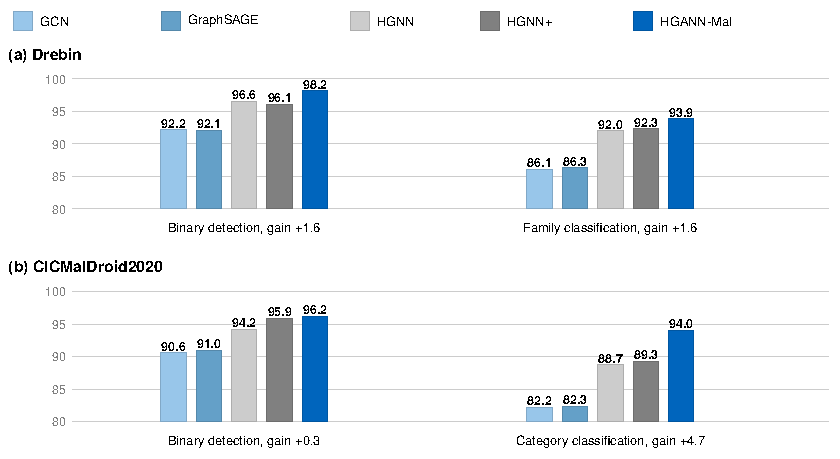
\includegraphics[width=\linewidth]{hgann-mal/hgann-mal-f1.pdf}
  \caption[F1 of the five methods on both corpora and both tasks]{F1 on both corpora and both
  tasks, as published in Tables~\ref{tab:hgann:binary} and~\ref{tab:hgann:multi}. The source labels
  these values Macro-F1, and Section~\ref{sec:hgann:14} shows that several rows cannot follow one
  averaging convention. The vertical axis is truncated at 80 so that differences among the
  hypergraph methods remain visible. HGNNP is the source publication's name for HGNN+.}
  \label{fig:hgann:f1}
\end{figure}

\begin{sidewaysfigure}
  \centering
  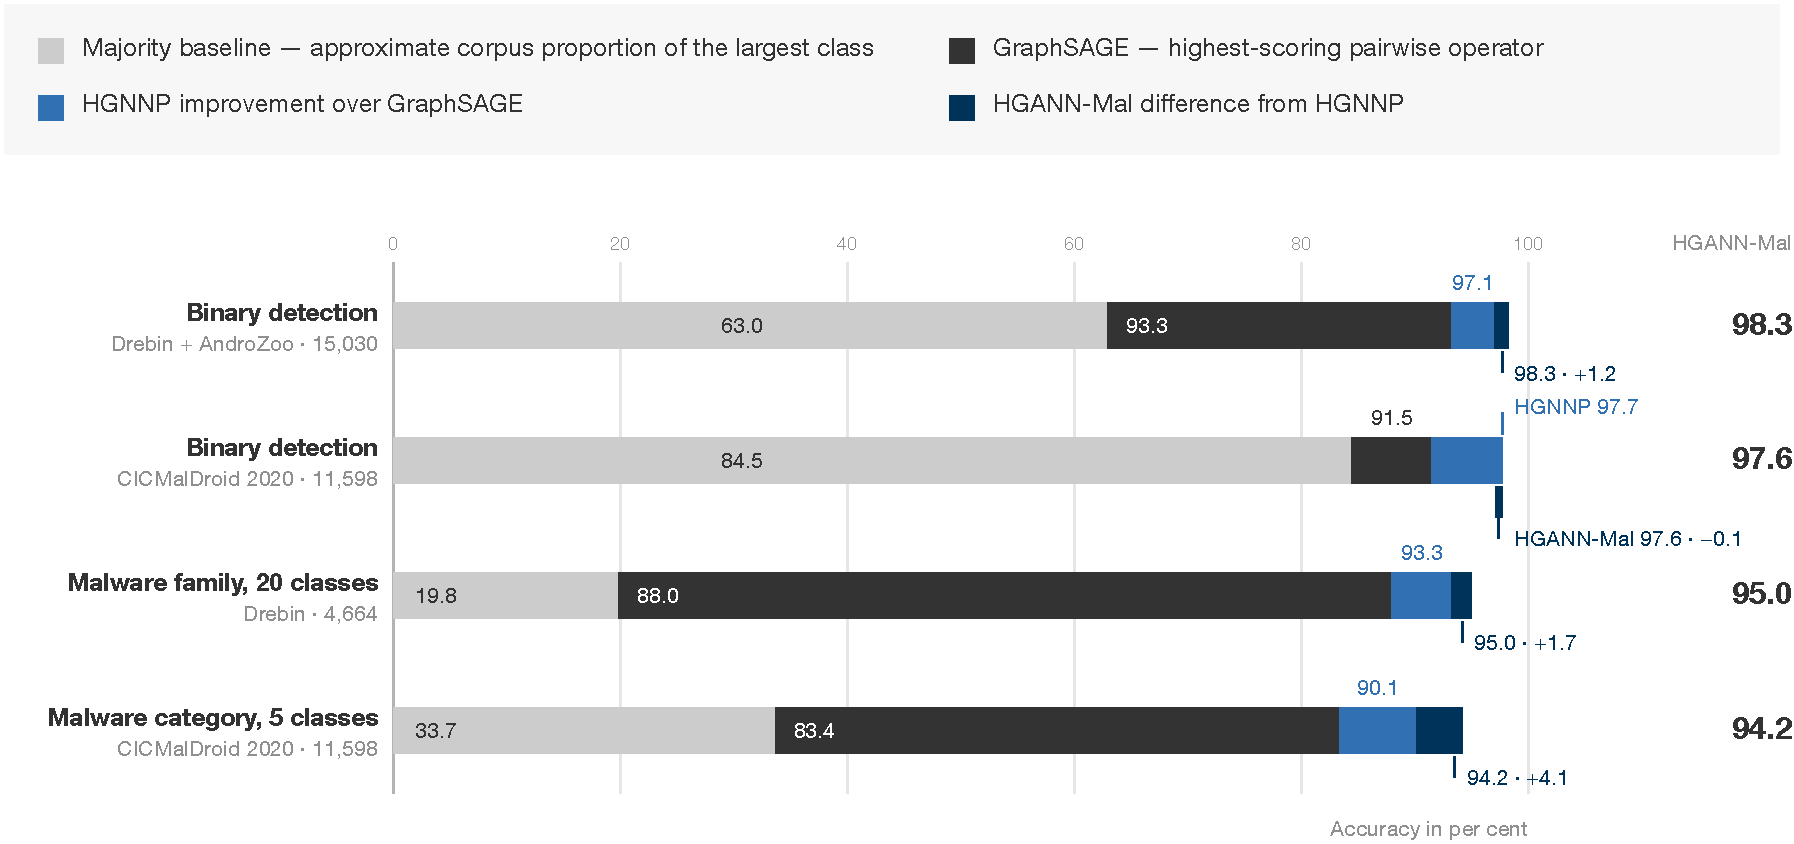
\includegraphics[width=\textheight]{hgann-mal/hgann-mal-accuracy.pdf}
  \caption[Accuracy against the majority baseline and the strongest baselines]{Accuracy reported
  in Tables~\ref{tab:hgann:binary} and~\ref{tab:hgann:multi}, divided at the majority baseline, at
  GraphSAGE and at HGNN+, which the figure labels HGNNP after the source publication. Variability
  across runs and the isolated contribution of attention are not established by these reported
  results.}
  \label{fig:hgann:accuracy}
\end{sidewaysfigure}

Three readings follow, and they are of unequal strength.

The clearest is the gap between the pairwise and the higher-order representations. On Drebin every
hypergraph operator sits above every pairwise one, by between 3.5 and 5.5 points of accuracy and
between 3.9 and 5.7 points of F1, and the ordering holds on CICMalDroid as well.
Figure~\ref{fig:hgann:accuracy} shows the same step on all four combinations: HGNN+ exceeds the
best pairwise operator, GraphSAGE in every case, by 3.8 to 6.7 points of accuracy, and in each
combination this step is larger than the difference between \hgann{} and HGNN+. All four
baselines were re-implemented on this pipeline and consumed the same call graph and the same node
features, so the difference belongs to
the representation rather than to the input. That is the comparison RQ3 asks for first, and it is
the one the evidence supports best.

The second is the gap between \hgann{} and the two hypergraph operators without attention. On
Drebin it is 1.2 points of accuracy against the stronger of them, and on CICMalDroid it is not
there at all: HGNN+ holds the best accuracy at 97.7 against 97.6, while \hgann{} holds the better
recall at 97.6 against 96.5 and the better F1 at 96.2 against 95.9. A system that leads on three
columns of four, and trails by one tenth of a point on the fourth, is level with its baseline on
that corpus rather than ahead of it. The source publication reads the same pattern as a
precision-recall trade-off, which is one explanation among several; single runs without dispersion
cannot separate a trade-off from noise, and Section~\ref{sec:hgann:14} returns to that.

The third concerns the base rate, and it is the reason the last row of the table is there. A
constant predictor scores 63.0 per cent on the Drebin corpus, where benign applications are the
majority, and 84.5 per cent on CICMalDroid, where they are 15.5 per cent of the samples. Reported
accuracy stands 35.3 points above the trivial baseline in the first case and 13.1 points above it
in the second. Neither figure is diminished by this, but the second is much less impressive than
97.6 per cent sounds, and the source publication reports no such baseline.

\subsection*{Drebin confusion matrix and class balance}

The Drebin binary experiment evaluated \hgann{} on 1,112 malicious and 1,894 benign applications.
The classifier identified 1,085 malware samples and missed 27. It raised 24 false alarms among
the benign applications and classified 1,870 as benign. These 51 errors across 3,006 decisions
give a false-positive rate of 1.3 per cent.

The experiment used a corpus with 37.0 per cent malware, whereas deployments may contain a lower
share. A separate sensitivity calculation holds recall and the false-positive rate fixed while
reducing the malware share to 10 per cent. Under this assumption, precision falls from 97.8 to
about 89.5 per cent because benign applications outnumber malicious applications nine to
one. This calculation illustrates the effect of class balance under fixed rates, as discussed in
Section~\ref{sec:background:evaluation}.

\section{Malware-Family Classification on Drebin}
\label{sec:hgann:11}

The second task assigns a malicious application to the family it belongs to. It runs on the 4,664
Drebin samples of the twenty largest families, shown in
Figure~\ref{fig:hgann:class-distribution}(a), and no
benign application takes part. Results are in the left panel of Table~\ref{tab:hgann:multi}.

\begin{table}
  \caption{Multiclass classification, in per cent, as published. The Drebin task assigns a
  malicious application to one of twenty families; the CICMalDroid task assigns an application to
  one of five categories, of which Benign is one. The two tasks are not comparable with each other.
  Section~\ref{sec:hgann:14} identifies two rows whose three columns cannot follow one averaging
  convention.}
  \label{tab:hgann:multi}
  \centering
  \begin{tabular}{lrrrr@{\hskip 2em}rrrr}
    \toprule
    & \multicolumn{4}{c}{Drebin, 20 families} & \multicolumn{4}{c}{CICMalDroid, 5 categories} \\
    \cmidrule(lr){2-5} \cmidrule(lr){6-9}
    Method & F1 & Prec. & Rec. & Acc. & F1 & Prec. & Rec. & Acc. \\
    \midrule
    GCN            & 86.1 & 85.9 & 86.2 & 87.8 & 82.4 & 82.0 & 82.4 & 82.7 \\
    GraphSAGE      & 86.3 & 86.7 & 86.2 & 88.0 & 82.3 & 82.2 & 82.6 & 83.4 \\
    \midrule
    HGNN           & 92.0 & 92.1 & 92.4 & 92.0 & 88.7 & 88.8 & 88.8 & 89.0 \\
    HGNN+          & 92.3 & 92.5 & 92.5 & 93.3 & 89.3 & 89.5 & 89.8 & 90.1 \\
    \hgann{}       & \textbf{94.2} & \textbf{94.1} & \textbf{93.8} & \textbf{95.0}
                   & \textbf{94.0} & \textbf{94.1} & \textbf{94.0} & \textbf{94.2} \\
    \midrule
    Majority class & & & & 19.8 & & & & 33.7 \\
    \bottomrule
  \end{tabular}
\end{table}

The ordering repeats: pairwise operators lowest, non-attentive hypergraph operators four to five
and a half points of accuracy above them, and \hgann{} 1.7 points above the better of those. Against
the trivial baseline the margin is wide here, since the largest family covers 19.8 per cent of the
samples.

One property of the task deserves more caution than the totals invite. The twenty families range
from 925 samples down to 41, a ratio above twenty to one. Read as a macro average, which is how
the source labels it, an F1 of 94.2 per cent would require the smallest families to be classified
nearly as well as the largest, since every class contributes equally to that average.
Section~\ref{sec:hgann:14} shows that the printed precision and recall of the same row exclude any
reading in which the three columns share one convention. The classes are also one vendor's
labels rather than an agreed taxonomy, as Section~\ref{sec:hgann:9} records, so a disagreement
between the model and the label is not always an error of the model. The families are further
related to one another: several of the twenty are known to contain repackaged applications built from shared
code. Shared code gives the applications of one family similar semantic hyperedges, each built
inside its own application under Section~\ref{sec:hgann:7}, and it is also the condition under
which duplication inflates a measured score. Section~\ref{sec:hgann:14} returns to that threat.

\section{Malware-Category Classification on CICMalDroid}
\label{sec:hgann:12}

The third task assigns an application to one of the five CICMalDroid categories. Benign is one of
them, so this task subsumes the detection question rather than sitting beside it, and an
application misclassified between two malicious categories is a different kind of error from one
misclassified as benign. Results are in the right panel of Table~\ref{tab:hgann:multi}.

The margin over the non-attentive operators is 4.7 points of F1 and 4.1 of accuracy, the widest of
the four task and corpus combinations reported anywhere in this chapter. The narrowest, on the
same corpus, is binary detection, where Section~\ref{sec:hgann:10} found no margin at all. The
ranking of the four combinations does not depend on the measure. Over the strongest baseline, the
F1 margins in Figure~\ref{fig:hgann:f1} are 4.7 points here, 1.9 and 1.6 on the Drebin family and
binary tasks and 0.3 on CICMalDroid binary detection, which is also the order of the accuracy
margins. That pattern is worth stating plainly because it constrains what may be concluded:
whatever the model
adds, it adds most where the decision is between several classes and least where it is between
two. A representation that groups methods by shared behaviour would plausibly help most in exactly
that setting, since categories such as adware and riskware are separated by what an application
does with what it collects rather than by whether it collects anything. The observation is offered
as a reading of the pattern and not as a finding, since one run per configuration cannot support
more.

\section{Ablation, Efficiency, and Interpretability Analysis}
\label{sec:hgann:13}

\subsection*{The ablation that was not run}

\hgann{} differs from the hypergraph baselines in two ways at once. It builds a different set of
hyperedges, fusing a topological, a semantic and a slice-aware family where the baselines take
$k$-hop and permission-based ones \cite{zhang2023android}, and it weights membership by a learned
score instead of a fixed indicator. Both changes are present in every number in
Tables~\ref{tab:hgann:binary} and~\ref{tab:hgann:multi}, and no experiment in this chapter varies
one while holding the other. The measured differences are therefore differences between two
systems, and they do not establish that attention is what produces them.

Four experiments would settle it, and they are recorded here so that the gap is specified rather
than merely admitted. First, the baseline operator without attention, run over the identical fused
hyperedge set, which isolates the aggregation. Second, \hgann{} run over topological hyperedges
alone, which isolates the vocabulary. Third, a leave-one-out over the three hyperedge families,
which apportions the vocabulary's contribution among them. Fourth, a sweep over $K$, $k$, $\tau$,
$c_{\max}$, $L_p$ and the two weight constants, none of which is varied anywhere in the source
publication. The first two are the ones that bear on RQ3; the second two would tell a reader how
sensitive the construction is to choices made once and never revisited.
Equation~\ref{eq:hgann:uniform} adds a condition to the first: uniform coefficients also rescale
propagation, so that comparison has to fix a normalisation convention before its difference can be
attributed to attention.

The question is not idle. On pairwise graphs, over node-property benchmarks and against
non-attentive baselines, no unmodified attentive model has been shown to outperform all of those
baselines on any dataset or task tested \cite{fang2025kaa}, and the scoring functions of both the
original and the revised formulations realise only finitely many neighbour rankings at bounded
width \cite{brody2022gatv2, fang2025kaa}. Neither result was stated for hyperedges, as
Section~\ref{sec:background:learning:attention} records. The static-ranking argument carries over
to the score used here, as Equation~\ref{eq:hgann:ranking} shows, while the finite-ranking bound
has not been examined for hyperedge scores. What the two results establish is that the attribution
cannot be assumed, and the evidence needed to make it was not gathered.

\subsection*{Efficiency}

The stated procedure admits bounds. Let $n$ be the number of methods, $m$ the number
of retained hyperedges, $\lvert \mathcal{S} \rvert$ the number of slices and
$\nu = \operatorname{nnz}(H) = \sum_{e \in \mathcal{E}} \lvert e \rvert$ the number of stored
memberships. Algorithm~\ref{alg:hgann:construction} proposes at most one topological and one
semantic candidate per method and one candidate per slice, and post-processing only removes
candidates. Semantic hyperedges hold at most $k + 1$ methods under the convention of
Equation~\ref{eq:hgann:sem}, and the others at most $c_{\max}$. Hence
\begin{equation}
  m \le 2n + \lvert \mathcal{S} \rvert , \qquad
  \nu \le (c_{\max} + k + 1)\, n + c_{\max} \lvert \mathcal{S} \rvert
  = 70\, n + 64\, \lvert \mathcal{S} \rvert ,
  \label{eq:hgann:sizes}
\end{equation}
and the representation grows linearly in the numbers of methods and slices. For one attention head
with input width $F$ and output width $F'$, a sparse evaluation of Equation~\ref{eq:hgann:attnprop}
computes the projection, the keys, the scores and the two incidence products in
\begin{equation}
  T_{\text{layer}} = O(nFF' + \nu F') , \qquad
  M_{\text{layer}} = O\bigl(nF + (n + m)F' + \nu + FF'\bigr)
  \label{eq:hgann:cost}
\end{equation}
time and memory, where $m \le \nu / 2$ because every retained hyperedge has at least two members.
The bound follows the two stages of Equation~\ref{eq:hgann:messages} and never forms
$P_{\text{att}}$. That matrix can be far denser than $H$, since two methods are coupled whenever
they share a hyperedge: it can hold up to $\sum_e \lvert e \rvert^2 \le c_{\max} \nu$ non-zero
entries, and the cap bounds this density. Further heads and layers add their own terms.

Construction costs more. With $\lvert E \rvert$ call edges, breadth-first searches from every
method build the topological hyperedges in $O(n(n + \lvert E \rvert))$. An exhaustive search within
one application evaluates the similarity of $O(n^2)$ pairs of 320-dimensional embeddings, and since
the FAISS index is unspecified, no sub-quadratic bound can be claimed for it. The slice paths need
one breadth-first search from each member of each slice,
$O\bigl(\sum_s \lvert F_s \rvert (n + \lvert E \rvert)\bigr)$ in total. The cap is applied after a
candidate is built, so it does not limit the cost of candidates that are then rejected, and
centrality computation and the semantic embedding add costs outside these bounds. None of these
quantities is a measurement. The claim in the source publication that the approach is inexpensive
because it is static is true of the analysis. For the representation, the bounds above are the only
evidence, and those for construction are quadratic in the number of methods.

\subsection*{Interpretability}

The slice-aware hyperedges are the part of the construction that could carry an explanation. Each
one is anchored at a call site of a security-sensitive API and covers the methods a backward slice
passes through, so an attention weight on such a hyperedge points at a concrete region of code and
at the API that made it interesting. Reporting the highest-weighted hyperedges for a sample, with
the call sites they contain, would turn a score into something an analyst can check.
Equation~\ref{eq:hgann:ranking} makes that report compact: within one layer and head every method
ranks its hyperedges by the same keys $b_e$, so one ranked list of keys per application summarises
what the layer attends to.

That was not done. The source publication states interpretability as future work, and no attention
weight is inspected, visualised or reported anywhere in it. A single retrained model on one corpus would be enough: the weights of
one application, ranked, with the API call at the anchor of each hyperedge, would turn this
section from a description of what the design permits into a result about what the model attends
to. It is named here because it is the cheapest substantial improvement available to the design,
and because the construction was built in a way that makes it reachable.

\subsection*{One design gap, and it is the cleanest extension available}

Section~\ref{sec:hgann:7} records that every hyperedge is tagged with the family that produced it,
and that the operator never reads the tag. A hyperedge reaches the layer as a column of $H$ and an
entry of $W$, so a topological hyperedge and a semantic one over the same methods are the same
object to the model, and only the slice-aware family is distinguished at all, through a weight it
happens to carry. The type is available, it is stored, and it is discarded.

Two ways of spending it suggest themselves. The weight matrix could carry a learned scalar per
family, so that the training decides how much a topological grouping is worth against a semantic
one, which costs three parameters. Or the attention score of
Equation~\ref{eq:hgann:attn} could take the type as an input. Entered additively, the type would
only shift the keys $b_e$, and Equation~\ref{eq:hgann:ranking} shows that every method would still
rank its hyperedges in one shared order; a weighting that depends on the family and the vertex
together needs a score that is not additive, such as the revised form of Brody et
al.\ \cite{brody2022gatv2}. Neither was tried here, and the second is the more
interesting because it is the version of the mechanism that the confound in
Section~\ref{sec:hgann:14} leaves unexamined.

\section{Limitations and Threats to Validity}
\label{sec:hgann:14}

The results above are measurements on two historical corpora under one protocol. This section
states the limits of what they show and closes with a brief account of threats to validity.

\paragraph{The gain cannot be attributed to attention.} \hgann{} changes the hyperedge vocabulary
and the aggregation together, and no experiment separates the two (Section~\ref{sec:hgann:13}).
The evidence supports a claim about the complete system: it performs better than four baselines on
three of the four task and corpus combinations. Whether learned weighting of hyperedges produces
that gain is an open question.

\paragraph{Every figure is a single run.} No configuration was repeated, and the tables therefore
carry no standard deviation, confidence interval or significance test. Small margins are affected
most. A tenth of a point separates \hgann{} from HGNN+ on CICMalDroid accuracy, and that difference
cannot be interpreted. Even the 1.2 points on Drebin would need repeated runs before they could be
called reliable.

\paragraph{The evaluation covers favourable conditions only.} Both splits are random, so training
and test samples come from the same collection period, and the figures do not describe performance
on applications released later \cite{pendlebury2019tesseract}. Neither corpus was obfuscated, and
no adversary was present. Under obfuscation, concept drift and adversarial examples, none of twelve
representative Android detectors kept the performance it reached in the ideal setting, and one
call-graph-based detector scored 0.912 of F1 on one year's test set and 0.463 on another's
\cite{gao2024comprehensive}. Sections~\ref{sec:hgann:10} to~\ref{sec:hgann:12} thus report the
conditions that a comparison between representations needs. A deployment would meet harder ones.

\paragraph{Some behaviour lies outside the representation.} Code fetched at runtime and targets
resolved by reflection are absent from the recovered call graph, and so are payloads held in packed
archives or native libraries (Section~\ref{sec:hgann:3}). A representation built from relations
among methods loses more from a missing method than one built from a bag of permissions.

\paragraph{The baselines are general operators.} GCN, GraphSAGE, HGNN and HGNN+ were
re-implemented on this pipeline's own representation. They test whether the higher-order encoding
and attention help within one design, but they do not place \hgann{} against the Android detectors
that the field uses as reference points. The hypergraph baseline has since been superseded by a
stability-oriented successor from the same group \cite{gao2026hgnnv2}, so the comparison reflects
that line of work as it stood in 2022.

\paragraph{The threat model is non-adaptive.} No adversary in this evaluation knows that the
detector exists, although published attacks act on the object this pipeline consumes. The first
structural attack on graph-based Android detection reports over 90 per cent success in feature
space and up to 100 per cent in problem space against function-call-graph detectors under
white-box access \cite{zhao2021structural}. FCGHunter rewrites an application with
semantics-preserving operators and reaches a white-box success rate of 87.9 per cent against forty
detectors built from graph-summary features \cite{song2026fcghunter}. A4M reports an average of
85.17 per cent against seven detectors built with MaMaDroid, APIGraph and a graph neural network,
under a perturbation budget of five per cent \cite{li2025efficient}. None of these attacks was run
against \hgann{}. Every hyperedge of Section~\ref{sec:hgann:7} is derived from the call graph or
from quantities computed over it, so methods and edges injected into that graph also change the
hyperedges. Attention operates downstream of an extraction that the adversary controls. \hgann{}
therefore inherits the exposure of its representation, and in line with Chapter~\ref{chap:advml}
this chapter makes no robustness claim.

\paragraph{Threats to validity.} The result tables head their first column Macro-F1 without stating
a convention. For the \hgann{} Drebin binary row a macro reading is impossible: over 1,112
malicious and 1,894 benign test applications, macro precision 97.8 and macro recall 97.6 at an
accuracy that rounds to 98.3 would require at least 1,897 true negatives. That row is read as
positive-class values. Under positive-class, macro and support-weighted averaging alike,
$F_1 \le (P + R)/2$, and four rows exceed that mean by more than the 0.1 point that rounding
allows: GCN and HGNN in the Drebin binary panel, \hgann{} in the \familyclassification{} panel, and
GCN in the \categoryclassification{} panel. No single convention fits these rows, so the
multiclass columns are not read as macro averages; accuracy is unaffected. On the data side, the
benign Drebin applications come from AndroZoo, which began crawling in late 2011, while Drebin
covers August 2010 to October 2012, so a classifier may separate the two collections by build tools
or API levels that have nothing to do with malice \cite{arp2022dos, allix2016androzoo}. The source
publication records that about 49 per cent of Drebin samples are repackaged applications, and none
was removed. Near-duplicates across the partitions may inflate the family scores of
Section~\ref{sec:hgann:11} more than the binary ones \cite{zhao2021impact, irolla2018duplication}.
CICMalDroid, for its part, keeps only applications that ran in its authors' sandbox
\cite{mahdavifar2020dynamic}, which may remove evasive samples that a static detector most needs
to catch.

\section{Chapter Summary}
\label{sec:hgann:15}

This chapter answered RQ3 by lifting a method-level function-call graph to a hypergraph, joining
its vertices by three rules of different kinds, and learning how strongly each method participates
in each group rather than fixing that strength when the structure was built. The system was
measured against two pairwise graph operators and two hypergraph operators without attention, on
Drebin and on CICMalDroid, for binary detection and for classification into families and into
categories.

Two findings hold. The higher-order representation is better than the pairwise one on every task
and corpus reported, by between three and eleven and a half points of accuracy depending on the
task and on which pair is compared, with the input to both held identical. The attention-weighted system is ahead of the non-attentive hypergraph
operators on three of four combinations and level on the fourth, and its widest margin appears on
the multiclass task rather than on detection. The analysis of Section~\ref{sec:hgann:8} sharpens
what the second finding can mean without adding evidence for it. Attention reweights the
memberships that the construction fixed, and within one layer it ranks the hyperedges of every
method in one shared order. A constructed example shows that it can still separate structures that
the fixed operator identifies, although nothing shows that training exploits this.

One thing does not hold, and the chapter states it rather than working around it. Because the
hyperedge vocabulary and the weighting were changed together, the improvement over the hypergraph
baselines cannot be attributed to attention, and the experiment that would separate them was not
run. Chapter~\ref{chap:discussion} takes the representational question up against
Chapter~\ref{chap:hybroid}, and Chapter~\ref{chap:conclusion} records the gap as the first item of
future work.
               % 5
\chapter{Evaluating Adversarial Robustness: Benchmark Design and Metric Analysis}
\label{chap:advml}

% Revised under T-003 and D-041 from notes/chapter6-source-records/.
% D-030 fixes RQ4; D-031 fixes attribution; D-009 fixes the grey-box convention.

\section{Research Problem and Contribution}
\label{sec:advml:1}

This chapter addresses RQ4: \rqFourText{} The question concerns gap~\gapref{4},
which links adversary assumptions to the validity of the resulting measurements.

Adversarial machine learning studies how deliberate changes to training data or inference
inputs can cause a learning system to fail, together with methods for resisting such changes
\cite{biggio2018wildpatterns}. A poisoning attack intervenes during training, whereas an
evasion attack modifies an input presented to an already trained model. Defences may expose
the model to adversarial examples during training, transform its inputs or internal
representations, or detect and respond to suspected adversarial inputs. This chapter concerns
evasion attacks and the evaluation of these three defence strategies. The broader attack
taxonomy and terminology are defined in Section~\ref{sec:background:adversarial}.

An empirical robustness estimate depends on the permitted perturbations and the attacks used
to search for them \cite{biggio2014security, carlini2019evaluating}. An unsuccessful search
may reflect resistance to the tested attack, or a failure of the attack to exploit the model.
For example, Athalye et al. identified obstructed gradients in seven of nine non-certified
defences accepted at ICLR~2018 and circumvented six completely and one partially
\cite{athalye2018obfuscated}. Evaluators therefore need to examine the measurement procedure
alongside the defended classifier.

The SPARTA SAFAIR work produced two complementary evaluation mechanisms: an adversarial
machine-learning competition and a reusable benchmark framework
\cite{sparta2021d73,sparta2022d76}. The competition evaluated submitted defences on hidden
test samples. The benchmark provided common interfaces for evaluating trained models against
reference attack implementations, with task-specific components for different prediction
problems. Its versioned source code is publicly available on GitHub
\cite{norouzian2021adversarialbenchmark}.

Using the project records, this chapter reconstructs both evaluation mechanisms and assesses
whether the reported measurements are consistent with the documented attack objectives,
attacker access and perturbation constraints. The empirical evidence comprises the contest
submissions and the application of the benchmark to partner defences on histopathology images.
The chapter then derives properties of the accuracy-loss score and the binary detector response
policy. These analytical results establish what the published aggregates support and what
additional observations would be required to distinguish competing explanations. A short
comparison with the project's PDF-malware study examines how feature constraints alter the
evaluation problem.

SPARTA was funded under Horizon~2020 grant agreement No.~830892. Its seventh work package,
SAFAIR, concerned the security of artificial-intelligence systems. The candidate wrote the
whole of D7.6, which reports the contest and benchmark, and Chapter~5 of D7.5
\cite{sparta2022d76, sparta2021d75}. Section~\ref{sec:advml:10} distinguishes this contribution
from the partner methods and experiments discussed below.

\section{Threat Analysis and Evaluation Scope}
\label{sec:advml:2}

SPARTA's threat analysis links attack techniques to affected ML assets and the adversary's
knowledge \cite[Sections~3.3.2--3.3.6]{sparta2021d71}. Applied to the evaluations in this
chapter, these distinctions locate the attack within the ML life cycle. Poisoning concerns
training data or the learning process; evasion concerns inputs supplied to a trained model.

The evaluations examined here concern evasion. The contest specified attacks that induce a
chosen identity or errors in selected facial attributes \cite[Section~3.3]{sparta2021d73}.
The histopathology benchmark reports classification accuracy on clean and perturbed images
\cite[Section~3.1.3]{sparta2022d76}. The affected asset is therefore the inference input, and
the measured outcome is prediction correctness under attack. Sections~\ref{sec:advml:3}
and~\ref{sec:advml:4} specify attacker access and permitted perturbations, which determine
the conditions under which these measurements can be interpreted.

\section{Evaluation Requirements and Threat Models}
\label{sec:advml:3}

The threat model specifies the attack objective, the information available to the attacker and
the operations permitted on the input. Section~\ref{sec:background:adversarial} fixes the
knowledge terminology used throughout the dissertation. Under its grey-box convention, some
model information is known and the training process cannot be influenced. Knowledge of
training data and the ability to alter those data are separate assumptions.

The contest granted knowledge of the training corpus, withheld the defence technique and model
architecture, and allowed gradient-based updates against the deployed model
\cite{sparta2021d73, norouzian2021safaircontest}. Access to gradients is an oracle capability.
The term grey box alone therefore leaves the experimental interface underspecified. The
conditions stated in Section~\ref{sec:advml:4}, including the query interface and input budget,
define the contest adversary used here. This is an academic evaluation setting; a survey of
271 practitioners found that academic knowledge assumptions often grant more information than
attackers have in deployment \cite{grosse2024towards}.

D7.3 adopted the evaluation checklist of Carlini et al. It called for attacks adapted to the
complete defence, explicit attack hyperparameters and comparisons with transfer or
gradient-free attacks. It also requested perturbation-budget curves and ablations
\cite{sparta2021d73, carlini2019evaluating}. These requirements provide a basis for assessing
the delivered results. Participation by independent attack teams can broaden the search, but
the scoring rule and the validity of each generated input require separate checks.

\section{Tasks and Evaluation Protocol}
\label{sec:advml:4}

\subsection{Prediction Tasks and Permitted Perturbations}

The contest specified an attack and a defence track for each of two tasks
\cite{sparta2021d73}. In targeted face re-identification, the attacker receives an image and
a target identity and attempts to induce that identity as the prediction. In attribute
alteration, the attacker receives a nominated subset of the forty binary facial attributes
and attempts to cause errors on that subset. A participant could attack one task and defend
the other, but could not enter both sides of the same task.

Let $f_\theta$ denote the model scores and $h$ the resulting class decision. For an image $x$
in a specified input coordinate system, define the feasible perturbations by
\begin{equation}
  \mathcal S_\varepsilon(x)
  =\{x'\in\mathcal X_{\mathrm{valid}}:\|x'-x\|_\infty\leq\varepsilon\}.
  \label{eq:advml:feasible}
\end{equation}
Here $\mathcal X_{\mathrm{valid}}$ includes the permitted pixel range and quantisation.
For pixel values scaled to $[0,1]$, the contest budget was $\varepsilon=8/255$, corresponding
to a maximum change of eight intensity levels per channel in the discrete $0$--$255$ encoding.
The rules required discrete output images, deterministic and stateless submitted models, and
an upper limit of four hours for generation of 1,000 perturbed examples
\cite{sparta2022d76}. The report identifies two 12~GB NVIDIA GPUs, a Titan~X Pascal and a
GeForce~GTX, with a 32-core AMD CPU and 128~GB RAM. Container execution used Ubuntu~18.04
and CUDA~10.1. These are reported resource limits, not measured per-example runtimes.

The budget must be interpreted before any model-specific normalisation. For example, a linear
rescaling from $[0,1]$ to $[-1,1]$ doubles the numerical distance. A reproducible evaluation
therefore records both the input coordinate system and preprocessing. The contest's
$8/255$ setting is not assumed for the histopathology results, whose attack configurations
are absent from the reported result table.

\subsection{Scoring and the Delivered Protocol}

SAFAIR ranked submissions by the change between clean and perturbed accuracy,
\begin{equation}
  \Delta=A_{\mathrm{initial}}-A_{\mathrm{final}}.
  \label{eq:advml:delta}
\end{equation}
Attacks sought the largest $\Delta$ and defences the smallest. Unless stated otherwise,
accuracies and $\Delta$ are proportions in this chapter; $100\Delta$ is a difference in
percentage points. D7.5 specifies clean accuracy and runtime as tie-breakers
\cite{sparta2021d75}. These do not prevent a low-utility model with a smaller $\Delta$ from
outranking a more accurate model.

The planned opening round evaluated defences against FGSM, BIM and PGD, with respective
weights $0.2$, $0.4$ and $0.4$ \cite{sparta2021d73}.
FGSM makes one update in the sign of the input-loss gradient
\cite{goodfellow2015explaining}. BIM repeats smaller
FGSM-style updates and clips each result to the permitted input range and perturbation
neighbourhood \cite{kurakin2017bim}. PGD also applies iterative gradient updates, projects
each result onto the feasible perturbation set, and can use multiple starting points
\cite{madry2018pgd}. Carlini--Wagner instead
formulates adversarial-example generation as an optimisation problem that balances the
required classification outcome against perturbation size \cite{carlini2017robustness}.
The five selected attacks would then face the five selected defences, with the final score
averaged over opponents \cite{sparta2021d73}. No attack submissions arrived. The organisers
used fixed baseline attacks instead; D7.5 lists Carlini--Wagner in addition to FGSM, BIM and PGD
\cite{sparta2021d75}. Table~\ref{tab:advml:designdelivery} records the
change in protocol.

\begin{table}[tbp]
  \caption{Planned and reported SAFAIR evaluation procedures.}
  \label{tab:advml:designdelivery}
  \centering\small
  \begin{tabular}{@{}p{0.20\linewidth}p{0.36\linewidth}p{0.36\linewidth}@{}}
    \toprule
    & \textbf{Plan} \cite{sparta2021d73} & \textbf{Reported delivery} \cite{sparta2021d75,sparta2022d76} \\
    \midrule
    Participants & attack and defence tracks for both tasks & defence submissions only \\
    Attack selection & organiser baselines, then five selected participant attacks & four named organiser baselines \\
    Defence score & weighted opening $\Delta$; mean final $\Delta$ over opponents & aggregate best and worst perturbed accuracies; $\Delta$ from the best value \\
    Final comparison & five attacks against five defences & no participant-attack round \\
    Reproduction & hidden evaluation set and submitted containers & sampling code and tool descriptions; incomplete run-level records \\
    \bottomrule
  \end{tabular}
\end{table}

The lack of independent attacks reduced the diversity of the evaluation. It does not explain
all weaknesses of the resulting measurement. As derived in Section~\ref{sec:advml:8:metrics},
a constant classifier has $\Delta=0$ against any set of label-preserving attacks, including
the opponents in the planned final round. The scoring defect and the attack-coverage defect
are therefore distinct.

The contest drew inspiration from the NIPS~2017 competition, whose defence score was the
proportion of correctly classified attacked images averaged across attacks
\cite{kurakin2018competition}. That score differs from Equation~\ref{eq:advml:delta}.
The competitions also differed in task and participation, so their results do not isolate
the effect of independent contestants. Details of the schedule are retained in the cited
project records; the scientific comparison here concerns the scoring and attack interfaces.

\section{Data and Evaluation Measures}
\label{sec:advml:5}

\subsection{Corpora and Hidden Evaluation Samples}

The contest used CelebA for model training, a corpus described by Liu et al. as approximately
200,000 images of 10,000 identities, with forty binary attributes per image
\cite{liu2015celeba}. For hidden attribute evaluation the organisers used LFWA, the
forty-attribute annotation of Labeled Faces in the Wild, which contains 13,233 images of
5,749 identities \cite{huang2007lfw, liu2015celeba}. A separate corpus reduces direct image
reuse, but does not establish equality of image distributions or attribute prevalences.

Re-identification required identity labels compatible with the trained classifier. The
organisers therefore used CelebA images under a random choice of colour jitter, greyscale
conversion, horizontal reflection or rotation of at most five degrees
\cite{sparta2022d76}. The printed procedure applies a face-detection check and retries failed
transformations before excluding an image. The resulting selection may differ from an
unfiltered sample. The report recognises that participants could have used similar
augmentations during training. Augmentation alone does not demonstrate independence from
training images.

The sampling code in D7.6 calls for 1,000 LFWA examples and, separately, 1,000 examples from
a re-identification test CSV. These are two task-specific samples. The code assigns
\texttt{random.seed = 42} instead of calling a seeding function, while the two pandas samples
receive no explicit random state. The augmentation draws are also stochastic. Consequently,
the printed procedure does not regenerate the exact hidden images. Saved manifests and
transformed files could establish their identity, but their recovery is not documented in
the deliverable \cite{sparta2022d76}.

\begin{table}[tbp]
  \caption{Evaluation units and data provenance. Stated sample sizes describe the printed
    procedures, not recovered per-example result files.}
  \label{tab:advml:data}
  \centering\small
  \begin{tabular}{@{}p{0.23\linewidth}p{0.33\linewidth}p{0.36\linewidth}@{}}
    \toprule
    \textbf{Evaluation} & \textbf{Input and prediction} & \textbf{Source and sampling} \\
    \midrule
    Contest identity & one image; one identity label & augmented CelebA; 1,000 selected test records \cite{sparta2022d76} \\
    Contest attributes & one image; forty binary labels & LFWA; 1,000 selected images \cite{sparta2022d76} \\
    Partner benchmark & one $50\times50$ histopathology patch; IDC/non-IDC & training, validation and test subsets described; evaluated subset size and patient separation unreported \cite{sparta2020d72} \\
    PDF comparison & 21 tag counts; benign/malicious & 20,000 files; 45/45/10 per cent defender/proxy/crafting split \cite{sparta2021d75} \\
    \bottomrule
  \end{tabular}
\end{table}

The histopathology corpus is identified in D7.2 as the IDC patch collection, whereas D7.6
calls it a breast-cancer image dataset without naming it \cite{sparta2020d72,sparta2022d76}.
The full collection contains 198,738 negative and 78,786 positive patches, so its majority
share is approximately $0.7161$ \cite{mooney2017idc}. The test subset's class share is not
reported. Neither this collection-wide ratio nor the contest's sample sizes can be used to
reconstruct the benchmark's confusion matrices.

\subsection{Accuracy and Task-Specific Attack Success}

For $N$ examples with identity labels $y_i$, the decision is
$h(x_i)=\arg\max_k f_{\theta,k}(x_i)$. Attribute decisions are
$h_j(x_i)=\mathbf1[f_{\theta,j}(x_i)\geq0]$ when the outputs are logits, with equivalent
threshold $0.5$ for sigmoid probabilities. The corresponding accuracies are
\begin{equation}
  A_{\mathrm{id}}=\frac1N\sum_{i=1}^N\mathbf1[h(x_i)=y_i],
  \qquad
  A_{\mathrm{attr}}=\frac1{40N}\sum_{i=1}^N\sum_{j=1}^{40}
                   \mathbf1[h_j(x_i)=y_{ij}].
  \label{eq:advml:accuracies}
\end{equation}
These conventions follow the task-specific scoring code printed in D7.6. Attribute accuracy
counts individual attribute decisions; it does not require all forty predictions for an
image to be correct \cite{sparta2022d76}.

Accuracy loss does not identify success against a specified target. For identity targets
$t_i\neq y_i$, let $I_t=\{i:h(x_i)=y_i,\ t_i\neq y_i\}$ contain eligible, initially correct
examples. Given valid attacked inputs $x_i'$, conditional targeted success is
\begin{equation}
  \mathrm{ASR}_{\mathrm{target}}
  =\frac{1}{|I_t|}\sum_{i\in I_t}\mathbf1[h(x_i')=t_i].
  \label{eq:advml:targeted}
\end{equation}
A prediction of a third identity reduces accuracy without satisfying the targeted objective.
An empty eligible set makes this rate undefined and its size must be reported.

For a nonempty nominated attribute subset $J_i$, define
$I_J=\{i:h_j(x_i)=y_{ij}\text{ for all }j\in J_i\}$. One explicit success criterion is
\begin{equation}
  \mathrm{ASR}_{\mathrm{subset}}
  =\frac1{|I_J|}\sum_{i\in I_J}\prod_{j\in J_i}
    \mathbf1[h_j(x_i')\neq y_{ij}].
  \label{eq:advml:subset}
\end{equation}
This requires errors on every nominated attribute of an initially correct subset. Reporting
$|I_J|$ separates induced errors from those already present; the rate is undefined if
$|I_J|=0$. Equations~\ref{eq:advml:targeted}
and~\ref{eq:advml:subset} specify measurements needed to evaluate the stated objectives;
they are not additional scores recovered from the contest. If an attack flips all $k$ initially
correct bits in the nominated subset and leaves all other decisions unchanged, the per-image contribution
to attribute accuracy falls by only $k/40$. For $k=1$ this is 2.5 percentage points, although
the specified attack succeeds.

\subsection{Aggregation over Attacks}

An attack suite can fail on different examples under each method. Selecting the lowest
aggregate accuracy does not account for that complementarity. Following per-example
evaluation guidance \cite{carlini2019evaluating}, let $\mathcal A_\varepsilon$ be a finite
set of attacks whose outputs satisfy Equation~\ref{eq:advml:feasible}. For a single-label task,
define
\begin{equation}
  \widehat A_{\mathcal A}(\varepsilon)
  =\frac1N\sum_{i=1}^N
   \min_{a\in\mathcal A_\varepsilon\cup\{\mathrm{id}\}}
   \mathbf1[h(a(x_i))=y_i].
  \label{eq:advml:suite}
\end{equation}
The identity transformation includes clean errors in the score. The suite must respect the
same threat model for each defence. Because it searches only a subset of valid perturbations,
its surviving accuracy is an upper bound on worst-case accuracy on these examples, not a
certificate of robustness. Moreover,
\begin{equation}
  \widehat A_{\mathcal A}(\varepsilon)
  \leq\min_{a\in\mathcal A_\varepsilon\cup\{\mathrm{id}\}}
           \frac1N\sum_i\mathbf1[h(a(x_i))=y_i],
  \label{eq:advml:aggregation-bound}
\end{equation}
since each per-example minimum is no greater than its value for any fixed attack.
The aggregate tables do not identify which examples fail under which attack, so this suite
score cannot be calculated retrospectively from them.

\subsection{Biometric Data and Data Protection}
\label{sec:advml:5:ethics}

The contest processed photographs of identifiable people and predicted identities or facial
attributes. D7.1 discusses purpose limitation, data minimisation and privacy by design, but
the contest documentation supplies no corpus-specific account of the lawful basis or the
participants' data-governance responsibilities \cite{sparta2021d71,sparta2022d76}. The
absence of that documentation establishes a reporting gap; it does not establish the consent
status of each person depicted or a legal finding about every possible use.

Attribute imbalance also affects the scientific interpretation. The SD account describes a
constant attribute predictor whose accuracy remains high because some attributes are rare
\cite{sparta2022d76}. A complete evaluation would therefore report attribute prevalences and
per-attribute outcomes alongside the aggregate score. Demographic performance differences
cannot be inferred from the reported aggregates. This chapter confines its empirical claims
to the documented classification tasks and does not infer suitability for biometric deployment.

\section{Benchmark Architecture and Reproducibility}
\label{sec:advml:6}

The benchmark implements a common software procedure for adversarial evaluation. It separates
attack execution from the task-specific model and data interfaces. D7.3 proposed five modules,
which D7.6 reports as implemented: attacks, datasets and models, together with use cases and a
wrapper \cite{sparta2021d73,sparta2022d76}. Figure~\ref{fig:advml:architecture} redraws the
published architecture.

\begin{figure}[tbp]
  \centering
  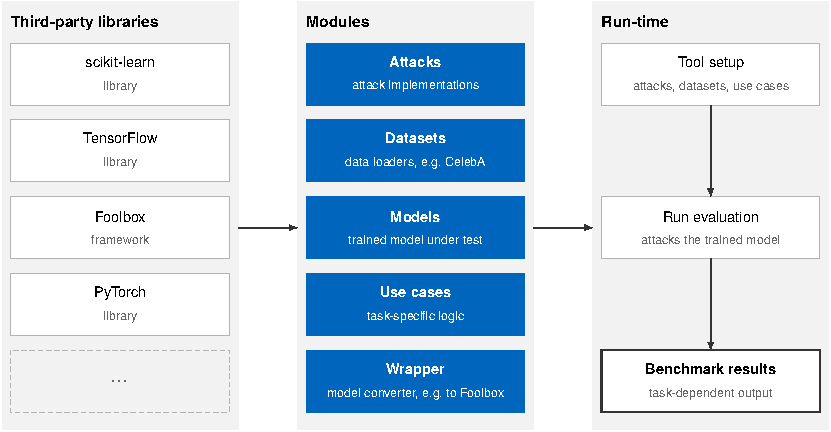
\includegraphics{sparta/thesis/sparta-benchmark-architecture.pdf}
  \caption{Benchmark architecture, redrawn after D7.6 Figure~2, p.~22 \cite{sparta2022d76}.
    Box labels follow the original. The second line in each box paraphrases the module and
    run descriptions in D7.6 Section~3.1.1. The five modules separate task definitions and
    data loading from attack execution. The diagram records the software design; it does not
    establish that a particular experiment preserved its model weights, data manifest and
    attack settings.}
  \label{fig:advml:architecture}
\end{figure}

Within this framework, standardisation concerns the component interfaces and execution
procedure. A run loads a trained checkpoint and evaluation data, converts the model to the
attack-library interface, measures performance before and after the selected attacks, and emits
the accuracies in one JSON-formatted result. Researchers can extend the procedure through new
attack classes and task-specific components. The implementation of this reusable workflow is
available in the versioned GitHub repository
\cite{norouzian2021adversarialbenchmark}.

The wrapper exposes a model through Foolbox, whose reference implementations supply the
attacks \cite{rauber2017foolbox}. PyTorch is the native model interface; the report also
describes conversion of TensorFlow or Keras models. Use-case classes select the prediction
criterion and loss for the task. A new attack extends a base class and is discovered by the
loader; a configuration list excludes named attacks. These interfaces permit reuse across
models. Compatibility still depends on the output semantics: the report's multi-label
wrapper handles fixed-budget attacks, while some minimum-distance interfaces are omitted
\cite{sparta2022d76}.

D7.6 also contains a description of splitting data and training classifiers, alongside repeated
statements that weights must already exist. The documented invocations require checkpoints,
and the inspected public implementation loads trained models
\cite{norouzian2021adversarialbenchmark}. Accordingly, the benchmark is described here as an
evaluation tool. Its public source is separate from the contest development toolkit
\cite{norouzian2021safairtoolkit}.

\paragraph{Perturbation validation.} The public revision identified by commit
\texttt{2fac62b947ed} pins Foolbox~3.3.1. Its attack call returns a raw candidate and a
budget-clipped candidate, with a success indicator. However, lines~134--135 of
\texttt{main.py} pass the raw candidate to the accuracy function
\cite{norouzian2021adversarialbenchmark}. In Foolbox's minimisation interface the clipped
candidate is obtained by restricting the raw perturbation to the requested distance budget;
the raw output need not satisfy that budget \cite{foolbox2021api}. Scoring the raw output
can therefore count changes outside the permitted set. This is a finding about the inspected
implementation. No recovered run record connects that revision to the histopathology table,
so it does not establish the cause of any historical result.

A further distinction concerns targeted runs. The same implementation replaces the reference
labels with the nominated target before computing its fields labelled accuracy. Those fields
then measure target-label agreement, with a different interpretation from true-label accuracy
\cite{norouzian2021adversarialbenchmark}. The examples in D7.6 Figure~6 likewise show a
targeted result whose value rises under attack \cite{sparta2022d76}. Each output therefore
needs an explicit task, reference label and denominator.

The inspected source fixes several dependency versions and allows the implementation to be
identified by a commit. Reproduction of a measured result additionally requires the exact
checkpoint and evaluation manifest, the preprocessing and attack parameters, and the individual
outputs. A valid evaluation would check quantisation and distances after all conversions,
record failed or skipped attacks, and score the candidate that satisfies the declared budget.
These are requirements derived from the interfaces, not claims that the historical runs
performed those checks.

\section{Defence Mechanisms and Integration}
\label{sec:advml:7}

The evaluated configurations instantiate the three defence strategies introduced in
Section~\ref{sec:advml:1}: adversarial training, transformations of inputs or internal
representations, and adversarial-input detection.

D7.6 evaluates five partner configurations described in D7.2. The underlying histopathology
classifier combines a pretrained VGG16 feature extractor with a dense prediction network
\cite{sparta2020d72,sparta2022d76}. Write its scores as
$f_\theta(x)=c_\psi(\phi_\omega(x))$, where $\phi_\omega$ is the convolutional feature
extractor and $c_\psi$ the prediction head. The following notation makes the intervention
of each defence explicit without supplying missing layer configurations.

\subsection{Training and Representation Transformations}

The adversarial-training configuration retrains the classifier with clean and perturbed
examples. D7.6 identifies FGSM, BIM and PGD as the attacks used to generate its adversarial
training examples \cite{sparta2022d76}. The surviving description does not specify the
mixture ratio or a complete optimisation schedule. This method exposes the model to those
attacks during training; resistance to other attacks remains an empirical question.

For the dimensionality-reduction variants, let $r_\eta$ denote an autoencoder. The two
configurations have score functions
\begin{equation}
  f_{\mathrm{top}}(x)=c_\psi\bigl(\phi_\omega(r_{\eta_x}(x))\bigr),
  \qquad
  f_{\mathrm{mid}}(x)=c_\psi\bigl(r_{\eta_z}(\phi_\omega(x))\bigr).
  \label{eq:advml:compositions}
\end{equation}
The first transforms pixels and the second transforms extracted features.
D7.2 states that the original convolutional network and prediction head retain their weights
in these autoencoder variants. Its separate encoder-only variant trains a new prediction
head, but that variant is not a column of the D7.6 benchmark table
\cite{sparta2020d72}. Figure~\ref{fig:advml:autoencoders} redraws the two published
placement diagrams in this notation.

\begin{figure}[tbp]
  \centering
  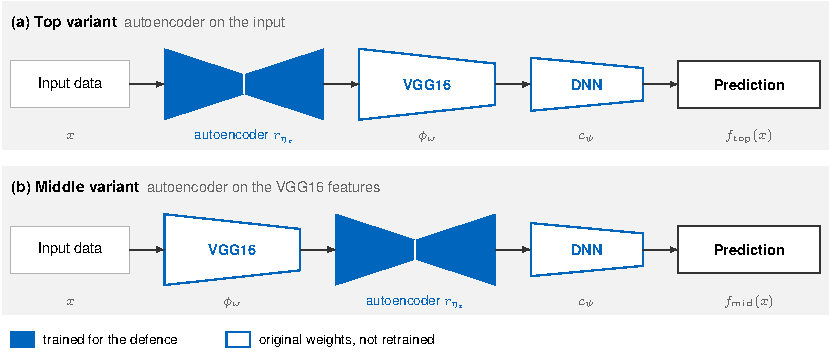
\includegraphics{sparta/thesis/sparta-autoencoder-placement.pdf}
  \caption{Autoencoder placement in the partner classifier, redrawn after D7.2 Figures~13
    and~11, p.~14 \cite{sparta2020d72}. In the top variant (a), the autoencoder
    $r_{\eta_x}$ transforms the input before feature extraction. In the middle variant (b),
    $r_{\eta_z}$ acts between the feature extractor $\phi_\omega$ and the prediction head
    $c_\psi$, as in Equation~\ref{eq:advml:compositions}. The legend follows D7.2, which
    keeps the original weights of VGG16 and the dense network in both variants. The
    diagrams specify placement, not a matched ablation of all training choices.}
  \label{fig:advml:autoencoders}
\end{figure}

A smaller reconstruction error alone does not establish robustness of either composition.
The relevant attack must optimise against the complete transformed classifier, including its
preprocessing. Reusing examples generated against the original classifier tests a different
condition from attacking the defended composition \cite{carlini2019evaluating}.

\subsection{History and Activation Detectors}

Figure~\ref{fig:advml:detectors} shows the two partner detectors and their response paths.

Prediction similarity adds a history of queries and their predictions. The partner study
records user information with image similarity and alarm statistics, and reports SSIM as the
similarity measure \cite{sparta2020d72}. Its alarm can be written
$d_t=d(x_t,H_{t-1})$, where $H_{t-1}$ contains the preceding queries associated with the
monitored interaction. A sequence of related optimisation queries may then trigger an alarm.
A transferred adversarial example submitted once presents a different observation to this
stateful detector.

For reproducibility, a history-based evaluation must specify the sequence order, user
association and reset policy. The contest's stateless-submission rule does not describe this
benchmark configuration. The reports do not establish a common history protocol across the
attacks in the result table, so their differences cannot be attributed solely to whether an
attack uses gradients.

The activation detector instead characterises the response of the underlying classifier to
an input. For each of nineteen hidden layers it calculates nine statistics: mean and median;
skewness and kurtosis; standard deviation and interquartile range; minimum and maximum;
and the number of nonzero activations \cite{sparta2020d72}. With layer activations
$a_\ell(x)$ and the statistic vector $s$, the representation is
\begin{equation}
  z(x)=\operatorname{concat}_{\ell=1}^{19}s(a_\ell(x))\in\mathbb R^{171}.
  \label{eq:advml:activation-features}
\end{equation}
After standardisation and feature selection, two support-vector classifiers are trained, one
for each class predicted by the original model. The selected detector therefore depends on
that prediction. The 94\% detector accuracy reported in D7.2 concerns detection of adversarial
inputs; it is not the defended task accuracy of the D7.6 table.

\begin{figure}[tbp]
  \centering
  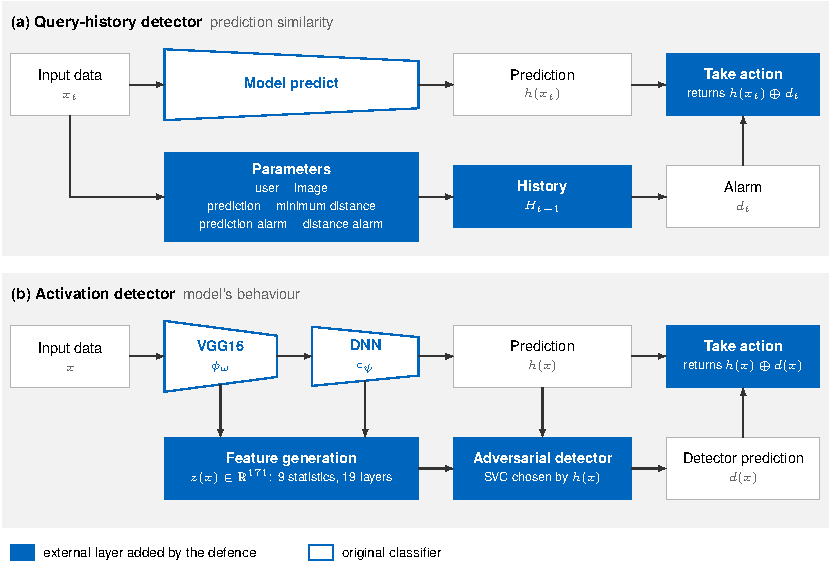
\includegraphics{sparta/thesis/sparta-detector-mechanisms.pdf}
  \caption{Partner detection mechanisms, redrawn after D7.2 Figures~15 and~16, p.~16
    \cite{sparta2020d72}. Panel (a) uses preceding queries, whereas panel (b) uses internal
    activations of the classifier. The recorded parameters, the activation features of
    Equation~\ref{eq:advml:activation-features} and the per-class detector follow D7.2.
    The response is the label reversal of Equation~\ref{eq:advml:reversal}, which D7.6
    applies in the benchmark \cite{sparta2022d76}. The final action is part of the defended
    system and must be included when task accuracy is measured.}
  \label{fig:advml:detectors}
\end{figure}

\subsection{From an Alarm to a Classification}

To place the detectors in an accuracy table, D7.6 uses the binary response policy of returning
the opposite class whenever the detector raises an alarm \cite{sparta2022d76}. Let
$h(x)\in\{0,1\}$ denote the base prediction, $d(x)\in\{0,1\}$ the alarm and $g(x)$ the
returned class. For a fixed history, where applicable,
\begin{equation}
  g(x)=h(x)\oplus d(x),
  \label{eq:advml:reversal}
\end{equation}
where $\oplus$ denotes exclusive OR. This rule corrects an erroneous binary prediction when
the detector raises an alarm, but turns a correct prediction into an error under the same
alarm. Consequently, on a common labelled evaluation set,
\begin{equation}
  A(g)-A(h)
  =\Pr(d=1,h\neq y)-\Pr(d=1,h=y).
  \label{eq:advml:reversal-gain}
\end{equation}
The probabilities denote empirical fractions on that set. To obtain the identity, partition
the observations by the alarm and the correctness of $h$: unflagged predictions are unchanged,
flagged errors are corrected, and flagged correct predictions are reversed. If $d(x)=1$ for
every observation, then $A(g)=1-A(h)$, while $g$ can still depend on the input.

Detection accuracy alone does not determine either term in
Equation~\ref{eq:advml:reversal-gain}. A useful evaluation records alarms jointly with base
and returned predictions, and measures false alarms on clean inputs. Abstention would be a
different response policy, for which coverage and error among accepted predictions must be
reported \cite{carlini2019evaluating}. The historical benchmark reports the reversal policy;
its aggregate accuracies do not identify the two joint fractions.

\section{Results and Metric Analysis}
\label{sec:advml:8}

\subsection{Contest Evidence}
\label{sec:advml:8:contest}

Table~\ref{tab:advml:contest} preserves the numerical columns of D7.6 Table~1. The source
reports one row per ranked team and task, rather than one row per submitted checkpoint.
Its surrounding text describes best and worst scores across submissions, but does not link
each value to an attack and checkpoint \cite{sparta2022d76}.

\begin{table}[tbp]
  \caption{Reported contest scores, including the worst-perturbed column, from D7.6 Table~1,
    p.~16 \cite{sparta2022d76}. Task names follow that table. The SD task label conflicts
    with its detailed attribute-model description; best and worst values are not identified
    as paired outcomes for one checkpoint under a common attack suite.}
  \label{tab:advml:contest}
  \centering\small
  \begin{tabular}{@{}llp{0.24\linewidth}cccc@{}}
    \toprule
    Rank & Team & Task & Clean & Best & Worst & $\Delta$ \\
    \midrule
    1 & SD & re-identification & 0.87 & 0.85 & 0.67 & 0.02 \\
    2 & Vicomtech & re-identification & 0.85 & 0.72 & 0.72 & 0.13 \\
      & Vicomtech & attribute alteration & 0.80 & 0.65 & 0.65 & 0.15 \\
    3 & BPI & re-identification & 0.84 & 0.68 & 0.68 & 0.16 \\
    \bottomrule
  \end{tabular}
\end{table}

The SD row reports 0.85 as best perturbed accuracy and 0.67 as worst, a spread of eighteen
percentage points. The printed $\Delta=0.02$ uses the best value. Subtracting 0.67 from 0.87
would give 0.20, but it would not establish a worst-case loss for the same model without the
missing checkpoint association. The report's prose also substitutes 87\% for attacked
accuracy and gives 61\% and 88\% values that do not match its table. The numerical record
used here is the table, with those inconsistencies retained as limits on interpretation.

The counts of submissions also disagree. D7.5 states seven defence submissions, six for
re-identification and one for attributes, whereas D7.6 states six submissions in total
\cite{sparta2021d75,sparta2022d76}. An unscored ITTI account appears in D7.6, but the
reports do not state that this explains the difference. Similarly, D7.5 gives SD a zero
$\Delta$ while D7.6 Table~1 gives 0.02. The development accounts describe models compatible
with different scores, but do not supply the identifiers needed to reconcile the two reports.

The four rows do not establish a general relation between clean performance and robustness.
They combine different prediction tasks and selected submissions from three teams. No
regression or significance test is appropriate for this table. D7.6 mentions ten-fold
cross-validation in the Vicomtech and BPI accounts, but does not provide fold assignments or
fold-level outcomes. Those statements cannot supply uncertainty estimates for the printed
scores.

\subsection{SD Development Configurations}
\label{sec:advml:8:sd}

D7.6 describes three SD models. Its introductory text assigns them to re-identification,
while the model details specify forty attribute outputs. The high accuracy of a constant
attribute vector cannot be interpreted as a demonstrated identity-classification result.
The following analysis therefore follows the attribute-model description and leaves its
mapping to Table~\ref{tab:advml:contest} unresolved \cite{sparta2022d76}.

The first configuration was a convolutional network trained on PGD examples with
$\varepsilon=0.3$, approximately 9.6 times the contest's $8/255$ budget if both use
$[0,1]$ pixels. The team reports that training produced the same output for every input,
with approximately 80\% clean attribute accuracy and zero accuracy loss. It attributes that
accuracy to the prevalence of absent attributes and recognises a weakness in the dataset
and contest rules. This is the source's direct account of prediction collapse, although
neither the checkpoint nor individual predictions accompany the reported result.

The second configuration combines six EfficientNet and three pruned ECA-ResNet models.
Their averaged outputs are thresholded to obscure gradients. For a nonzero scalar attribute
logit $u$, write the transformation as
\begin{equation}
  q(u)=\begin{cases}10,&u>0,\\-10,&u<0.\end{cases}
  \qquad
  \mathbf1[q(u)\geq0]=\mathbf1[u\geq0],
  \qquad q'(u)=0\ \ (u\neq0).
  \label{eq:advml:threshold}
\end{equation}
The source does not specify the exact-zero tie. Away from that tie, the operation preserves
the binary decision and suppresses its direct derivative. It can obstruct a gradient-based
attack without changing the classifier's decision regions. Attacks adapted to the
non-differentiable operation or transferred from another model remain relevant
\cite{athalye2018obfuscated, tramer2020adaptive}.

The second configuration achieved approximately 92\% clean accuracy and 79\% under
transferred attacks in the team's development account. The third used one pruned ECA-ResNet,
added adversarial training, and retained the threshold operation. Its reported clean
accuracy was approximately 87\%, with 84--85\% under transferred attacks
\cite{sparta2022d76}. Figure~\ref{fig:advml:sd} shows these values separately from the
contest table.

\begin{figure}[tbp]
  \centering
  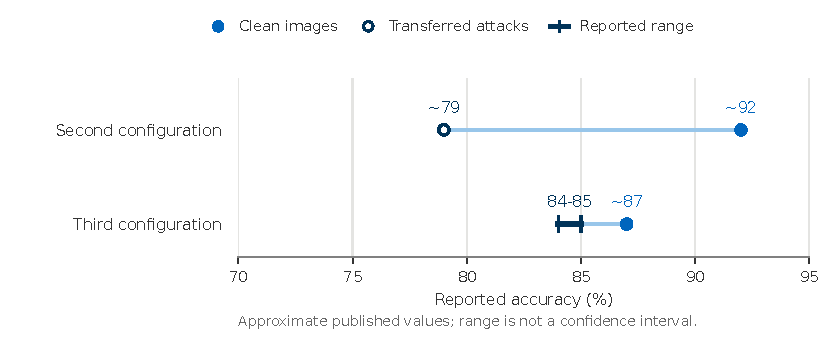
\includegraphics[width=\linewidth]{sparta/thesis/sparta-sd-comparison.pdf}
  \caption{SD development configurations from D7.6 Sections~2.8.1.2--2.8.1.3, pp.~18--19
    \cite{sparta2022d76}. The interval 84--85\% is a reported approximate range, not a
    confidence interval. The source describes attribute outputs despite its re-identification
    heading. These values are not additional official contest rows.}
  \label{fig:advml:sd}
\end{figure}

The third configuration trades five percentage points of reported clean accuracy for five to
six points of transferred-attack accuracy relative to the second. This is a descriptive
comparison between systems: ensemble size and training changed together, and the attacks'
individual settings are not given. It does not isolate the effect of adversarial training.
The transfer results nevertheless show why resistance to a direct gradient attack is an
incomplete measure of these constructions.

\subsection{Histopathology Benchmark}
\label{sec:advml:8:benchmark}

D7.6 reports that Vicomtech used the benchmark tool to evaluate five defence configurations
on a histopathology classification task \cite[Section~3.1.3]{sparta2022d76}. This application
documents use of the framework for a prediction problem distinct from the competition's facial
image tasks. Table~\ref{tab:advml:benchmark} reproduces the reported accuracies for binary IDC
classification. For the two detectors, these include the response policy in
Equation~\ref{eq:advml:reversal}. The clean row records the prediction cost associated with
each configuration.

\begin{table}[tbp]
  \caption{Published accuracies for the five partner defence configurations, from D7.6
    Table~2, pp.~28--29 \cite{sparta2022d76}. Attack hyperparameters and the evaluated
    subset are unspecified. Each entry is a reported aggregate, with no dispersion estimate.}
  \label{tab:advml:benchmark}
  \centering\small
  \begin{tabular}{@{}lccccc@{}}
    \toprule
    Attack & Adv.\ training & Top AE & Middle AE & Pred.\ similarity & Activations \\
    \midrule
    none (clean) & 0.844 & 0.726 & 0.817 & 0.844 & 0.708 \\
    FGSM & 0.837 & 0.716 & 0.812 & 0.837 & 0.708 \\
    $L_2$ basic iterative & 0.844 & 0.725 & 0.817 & 0.842 & 0.708 \\
    BIM & 0.837 & 0.716 & 0.812 & 0.837 & 0.708 \\
    DeepFool & 0.003 & 0 & 0.001 & 0.015 & 0.708 \\
    additive noise & 0.844 & 0.725 & 0.817 & 0.844 & 0.708 \\
    NewtonFool & 0.464 & 0 & 0 & 0.460 & 0.708 \\
    PGD & 0.837 & 0.717 & 0.813 & 0.837 & 0.708 \\
    \bottomrule
  \end{tabular}
\end{table}

The middle autoencoder exceeds the top autoencoder by 9.1 percentage points on clean data
and 9.6 points under the reported PGD condition. Its PGD loss is 0.4 points, compared with
0.9 for the top variant. These values favour the middle configuration within the reported
evaluation. They do not establish that placement alone caused the difference, because the
complete training configurations and repeated-run outcomes are unavailable.

Adversarial training and prediction similarity have equal reported clean accuracy and equal
FGSM, BIM and PGD values. Prediction similarity is higher under DeepFool by 1.2 percentage
points, but lower under NewtonFool by 0.4 points. It therefore does not dominate adversarial
training across the table. The source's explanation that similarity detects gradient-based
construction is insufficient to explain the results, since DeepFool and NewtonFool also use
gradient information. Query sequences and detector alarms would be needed to test that
mechanism.

The activation column remains at 0.708, including on clean inputs. This establishes equality
of the printed aggregates to their reported precision. It does not establish identical
predictions, an always-active detector or insensitivity to inputs. The full corpus's majority
share is approximately 0.7161, but the unknown evaluation split prevents a matched baseline
comparison. Equation~\ref{eq:advml:reversal-gain} also shows that always reversing predictions
would not, by itself, yield the class prior. The mechanism behind the column remains
unidentified.

The near-zero DeepFool results for four configurations require a different qualification.
Minimum-distortion attacks search for an adversarial input and should be compared by the
distortion required, or by success after imposing a common valid budget
\cite{moosavi2016deepfool,carlini2019evaluating}. Neither the norm and stopping settings nor
achieved distortions are reported for these benchmark runs. The table therefore cannot
establish that its attack rows represent equally constrained adversaries. The code finding
in Section~\ref{sec:advml:6} reinforces the need to validate distances, but does not resolve
the historical configuration. The additive-noise row is a useful control condition; without
its distribution, budget and number of trials, its small changes do not establish a
comprehensive random-search check.

\subsection{Sensitivity to the Scoring Rule}
\label{sec:advml:8:metrics}

Figure~\ref{fig:advml:deltas} subtracts each attacked accuracy from that configuration's
clean accuracy. It makes the score dependence visible without changing the original results.
Under PGD, the activation detector has the smallest $\Delta$, zero, but its attacked
accuracy is 12.9 percentage points below adversarial training. Similarly, the middle
autoencoder has a smaller loss than adversarial training while its attacked accuracy is
2.4 points lower. A smaller loss alone therefore does not identify the more useful defended
classifier.

\begin{figure}[tbp]
  \centering
  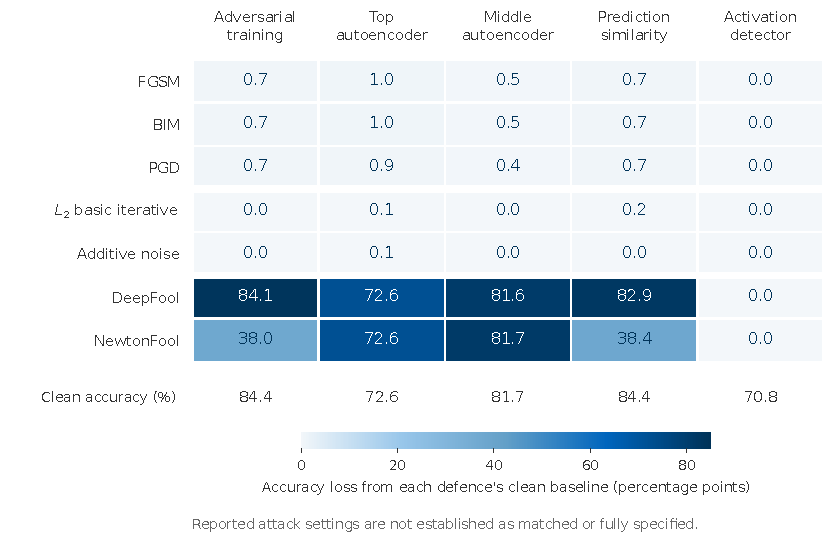
\includegraphics[width=\linewidth]{sparta/thesis/sparta-benchmark-deltas.pdf}
  \caption{Accuracy losses computed from D7.6 Table~2 \cite{sparta2022d76}. Each cell is
    $100(A_{\mathrm{clean}}-A_{\mathrm{attack}})$ in percentage points; the original
    accuracies remain in Table~\ref{tab:advml:benchmark}. The separation of attack rows
    does not imply matched budgets. In particular, zero loss for the activation detector
    describes its aggregate score, not a demonstrated mechanism or robustness certificate.}
  \label{fig:advml:deltas}
\end{figure}

For paired clean and attacked examples, let $C$ denote an initially correct prediction and
$C'$ a correct prediction after attack. Expanding the two accuracy terms yields
\begin{equation}
  \Delta=\Pr(C\cap\neg C')-\Pr(\neg C\cap C').
  \label{eq:advml:cancellation}
\end{equation}
Both accuracies contain the correctly classified observations in $C\cap C'$, which cancel.
Thus, $\Delta$ measures the net change in correctness. It is not the conditional fraction
of initially correct examples made incorrect. Equal numbers of harmful and corrective
changes can leave $\Delta=0$ despite changes in individual outcomes. The aggregate table
cannot determine those two counts.

\paragraph{Constant-prediction result.} For any constant classifier $h_c(x)=c$ and
label-preserving attack $a$, $h_c(a(x_i))=h_c(x_i)$ for each observation. Therefore,
\begin{equation}
  A_{\mathrm{clean}}(h_c)=A_{\mathrm{attack}}(h_c)
  =\widehat p_c,\qquad \Delta(h_c)=0,
  \label{eq:advml:constant}
\end{equation}
where $\widehat p_c$ is the evaluated class fraction. The statement holds for each attack
and any weighted average over attacks. Independent opponents cannot eliminate this property
of the score. The result establishes an indifference to prediction utility when ranking
only by loss; it does not imply that the constant classifier correctly classifies the other
classes.

For attributes, choose a fixed vector $m$ using training-set majority labels. Its held-out
accuracy is
\begin{equation}
  A_{\mathrm{attr}}(m)
  =\frac1{40}\sum_{j=1}^{40}
    \bigl[m_j\widehat p_j+(1-m_j)(1-\widehat p_j)\bigr],
  \qquad \Delta(m)=0,
  \label{eq:advml:constant-attributes}
\end{equation}
where $\widehat p_j$ is the prevalence of attribute $j$ in the evaluation set. When the
training and evaluation majorities agree, each summand is
$\max(\widehat p_j,1-\widehat p_j)$. This explains how a fixed attribute vector can have
high average accuracy on an imbalanced corpus. The baseline labels must be fixed before
evaluation; selecting them from hidden test labels would use unavailable information.

These identities support reporting clean utility together with attacked performance and a
matched constant baseline. Prediction distributions and paired error transitions provide
additional checks. None of these quantities can be reconstructed uniquely from an unchanged
accuracy column, so the activation result remains an observation rather than a second
demonstration of the SD collapse mechanism.

\subsection{Comparison with Constrained PDF-Malware Features}
\label{sec:advml:8:pdf}

The public D7.5 report contains a partner study of evasion against PDF-malware classifiers
\cite{sparta2021d75}. It provides a comparison with the continuous image setting, rather
than an additional experiment on the Android systems in this dissertation. The study uses
10,000 benign and 10,000 malicious Contagio files. PDFiD extracts 21 tag counts; the data
are partitioned into 45\% for defender training, 45\% for proxy training and 10\% for
adversarial crafting. A neural proxy generates examples transferred to neural, SVM and
random-forest classifiers, without queries to the target during generation.

The allowed changes increase tag counts and preserve integer values after inverse
standardisation and rounding. If $v\in\mathbb N_0^{21}$ is the original count vector,
the reported feature constraints require
\begin{equation}
  v'\in\mathbb N_0^{21},\qquad v'_j\geq v_j\quad(j=1,\ldots,21).
  \label{eq:advml:pdf-constraints}
\end{equation}
A perturbation bound also applies in the attack representation. Its interpretation depends
on standardisation and the subsequent rounding. These constraints restrict the feature
search, but do not establish that a corresponding modified PDF was constructed or that its
malicious functionality was preserved. The distinction is the feature-space versus
problem-space distinction of Section~\ref{sec:background:adversarial}.

\begin{figure}[tbp]
  \centering
  \begin{subfigure}[t]{0.49\linewidth}
    \centering
    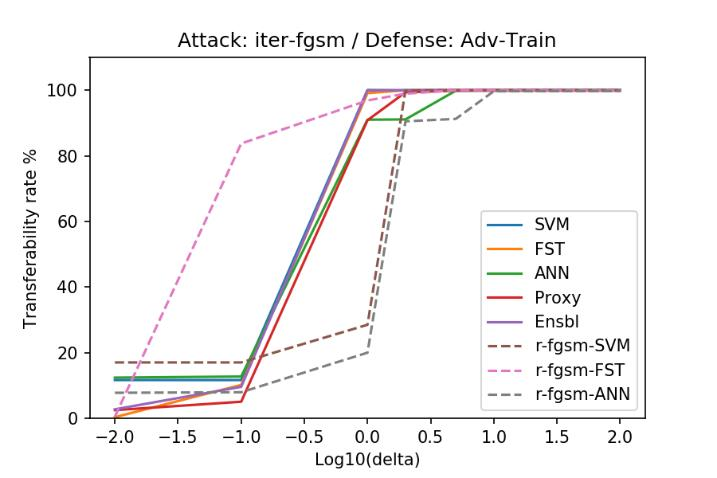
\includegraphics[width=\linewidth]{sparta/report-originals/d75-fig15-iter-fgsm-left.jpg}
    \caption{Adversarial training.}
  \end{subfigure}\hfill
  \begin{subfigure}[t]{0.49\linewidth}
    \centering
    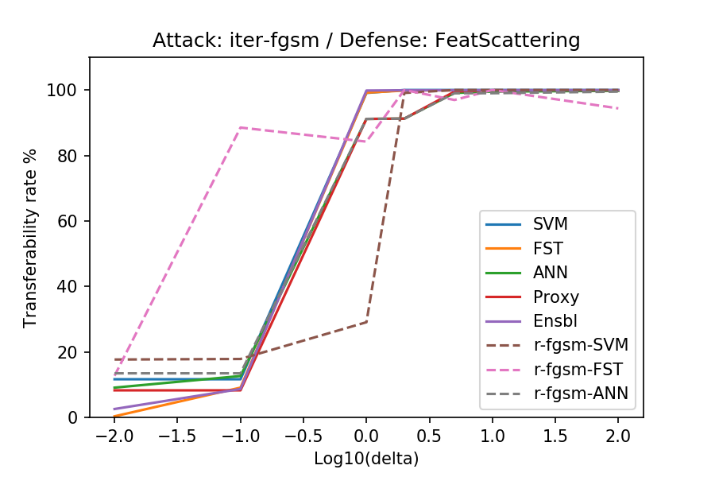
\includegraphics[width=\linewidth]{sparta/report-originals/d75-fig15-iter-fgsm-right.png}
    \caption{Feature scattering with adversarial training.}
  \end{subfigure}
  \caption{Original iterative-FGSM transfer curves from the partner PDF-malware study,
    D7.5 Figure~15, p.~23 \cite{sparta2021d75}. Both panels retain the published legends
    and values. The horizontal axis is the source's $\log_{10}(\delta)$ perturbation
    budget, distinct from the accuracy loss $\Delta$ used in this chapter. These are
    feature-space results, with no uncertainty bands or demonstrated construction of
    modified PDFs with preserved malicious functionality.}
  \label{fig:advml:pdf-transfer}
\end{figure}

The retained legend names the SVM, random forest (FST), neural network (ANN) and their
ensemble (Ensbl); the prefix r-fgsm denotes adversarial retraining with FGSM examples.
Proxy measures success against the attack's source model, rather than cross-model transfer.
In the feature-scattering condition the SVM and random forest receive adversarial
augmentation, so that panel represents a hybrid defence comparison \cite{sparta2021d75}.

In Figure~\ref{fig:advml:pdf-transfer}, transfer success for many reported models rises
sharply as the budget increases, and several approach 100\% at larger budgets. Other curves
are non-monotone. Such curves record the success of the specified search at each setting;
they do not establish the monotone worst-case envelope over nested feasible sets. The two
panels also show dependence on the target model and defence configuration. They support
reporting a budget-dependent curve with explicit constraints, while the limited settings
and absent repeated-run information prevent a general ranking of defence families. The
same methodological requirement applies to Android: an evaluation must state how permitted
artefact transformations map to the representation used by the detector.

\section{Threats to Validity}
\label{sec:advml:9}

\paragraph{Measurement validity.} The contest combines task-dependent accuracies with a
net-change score. The identity and attribute objectives require different success criteria,
and the targeted software output uses target-label agreement. Aggregate accuracy loss
cannot identify induced errors, useful classification or detector alarms. The analytical
results in Sections~\ref{sec:advml:7} and~\ref{sec:advml:8:metrics} identify these limits;
they do not recover unreported individual outcomes.

\paragraph{Attack coverage and budgets.} No independent attack submissions entered the
contest. Its fixed gradient-based baselines did not constitute a documented adaptive
assessment of every defence. The SD development account includes transfer attacks, but
the official table provides no per-attack breakdown. The benchmark additionally mixes
attack families without the full configurations needed for comparison. A later evaluation
would require valid perturbations in common coordinates and attacks adapted to the complete
defended system, with convergence checks \cite{carlini2019evaluating,tramer2020adaptive}.

\paragraph{Sampling and uncertainty.} The printed hidden-set procedure has unseeded draws
and stochastic transformations. Augmentations do not establish absence of overlap with
training images. The histopathology subset size, class proportions and patient-level
partitioning are unreported. Patch counts cannot be treated as independent patient counts,
and forty attributes on the same image are dependent observations. The available rounded
aggregates and statements about cross-validation do not support confidence intervals,
paired significance tests or a fitted clean--robustness relation.

\paragraph{Conflicting records and implementation provenance.} The SD task names and the
submission totals disagree across the reports. No checkpoint mapping resolves the zero
and 0.02 deltas or the best and worst score associations. The inspected code exposes a
raw-versus-clipped scoring issue, but its connection to the published experiment is unknown.
The source repository and dependency versions therefore support implementation inspection,
while experiment reproduction still requires the corresponding data and model artefacts.
These distinctions remain explicit rather than being resolved by a presumed run history.

\paragraph{Generalisation and attribution.} The four participating teams belonged to SPARTA,
so the contest did not test participation beyond the consortium. The evaluated image tasks
also differ from Android malware analysis in their inputs and validity constraints. The
public PDF-malware study narrows this conceptual difference through constrained count
features, but supplies no Android result. Its experiments and the partner defence algorithms
retain their attribution. D7.4 is a confidential deliverable; the figures and empirical
comparisons in this chapter use public reports.

A focused subsequent study could compare an ordinary classifier with a training-selected
constant baseline and the same classifier under output thresholding. For detectors, paired
base predictions and alarms would test Equation~\ref{eq:advml:reversal-gain}. Budget curves
and per-example attack aggregation would then measure how the conclusions change under
validated perturbations. Those experiments remain separate from the historical evidence
presented here.

\section{Individual Contribution and Project Attribution}
\label{sec:advml:10}

The candidate's contribution is stated at section level, following his account of the
collaborative project. He wrote D7.1 Sections~2.2.2 and~2.3, and D7.2 Sections~2.1 and~2.2.
For D7.2 Sections~2.4 and~2.5 he contributed the concept and definitions. He edited and
refined partner text in D7.3, with no authored content claimed for that plan. He wrote
Sections~3.1 and~3.2 of D7.4, Chapter~5 of D7.5, and the whole of D7.6
\cite{sparta2021d71,sparta2020d72,sparta2021d73,sparta2021d75,sparta2022d76}.
His D7.4 contribution is recorded as part of this account, without using the confidential
report as an empirical source.

Within SAFAIR, the candidate contributed to organising the competition and to developing the
reusable benchmark framework. The contest toolkit and benchmark source code are published on
GitHub under the candidate's name
\cite{norouzian2021safairtoolkit,norouzian2021adversarialbenchmark}. The evaluated defensive
algorithms remain partner methods. In particular, the histopathology configurations originate
in the Vicomtech study of D7.2 Section~2.3.2; the PDF-malware curves belong to the partner
study in D7.5 Section~2.8. Authorship of the reporting deliverables does not transfer those
experiments or algorithms to the candidate. The mathematical analysis and source comparison
in this chapter examine their implications for the evaluation framework.

\section{Chapter Summary}
\label{sec:advml:11}

RQ4 concerns the translation of an adversary model into a reproducible benchmark and the
relation between clean performance and adversarial robustness. The SAFAIR work delivered a
competition with hidden evaluation samples and a reusable framework for evaluating trained
models against reference attacks. The framework established common component interfaces and
an execution procedure with adaptations for different prediction tasks. Its reported use by
Vicomtech on histopathology images documents an application separate from the competition.
The subsequent analysis identifies the experimental records and measurement checks required
to interpret the resulting scores.

The evidence supports several bounded conclusions. The histopathology table gives different
comparisons under accuracy loss and absolute attacked accuracy. The SD development account
reports improved transfer-attack performance in a configuration with lower clean accuracy,
but changes in ensemble size and training prevent causal attribution. The constant-prediction
result proves that the historical delta score can assign zero loss to a classifier with low
utility. Logit thresholding provides a separate mechanism: the attribute decisions remain
unchanged while direct gradients are obstructed. The invariant activation-detector accuracy
does not identify either mechanism.

These findings support an evaluation that reports clean and attacked utility together, tests
attacks against the full defence, and records individual predictions with valid perturbation
budgets. For detector-based systems, the response to an alarm is part of the method being
evaluated. The constrained PDF example further shows why the validity of an input must be
specified for its domain. The chapter establishes these methodological consequences from
the documented systems and their measurements, while leaving a general clean--robustness
relation and experiment-level reproduction unresolved.
  % 6
\chapter{Cross-Contribution Discussion}
\label{chap:discussion}

% Drafted under T-004 from the current text of Chapters 3 to 6, and revised on 11 September 2026
% from the author's proposed text (tmp/chapter7-review/chapter7-proposed.md). Constraints from
% notes/dissertation-structure-v0.3.md: the comparison is conceptual, no result of Hybroid is
% compared numerically with a result of HGANN-Mal, and no developmental sequence from the IoT
% work to the Android work is claimed. Section 5.3 cites sec:discussion:3 by label.
% Length fixed at four pages by D-044.

The contribution chapters examine different forms of context under separate experimental
protocols. This discussion relates the observations each representation requires to the
conclusions its evaluation supports. Comparisons between \hybroid{} and \hgann{} are conceptual;
their scores do not provide a direct comparison because the corpora and tasks differ. The central
question is when additional context provides useful information and how the evidence for that
benefit is bounded.

\section{Communication Context and Program Context}
\label{sec:discussion:1}

In the network studies of Chapter~\ref{chap:anomaly}, context comprises the communication
partners of a device or service and the exchanges observed between them. In \hgann{}, context
consists of relations among methods within an application. \hybroid{} combines program structure
with network observations. Each representation depends on its observation process: the service
graph contains relations encountered during learning, whereas the call graph contains
invocations recovered by static analysis. Neither is a complete record of system behaviour. This
comparison concerns their methodological properties; it does not imply a developmental link
between the IoT and Android studies.

Legitimate changes can also produce anomalous observations. Each of the nine false alarm episodes
on the industrial benign monitoring day had a benign cause. Three followed engineering
workstation activity and two followed planned device restarts. The service-graph design
permits an operator to approve new relations. An application update that changes its call graph
presents a related problem, but the Android evaluations did not examine it. The industrial
observations therefore motivate a question about adaptation to legitimate change, without
demonstrating its effect on either Android detector.

\section{Multimodal and Higher-Order Representations}
\label{sec:discussion:2}

Both Android systems derive method-level call graphs with Androguard and use opcode information
with operands discarded. \hybroid{} adds traffic captured from the application. \hgann{}
constructs hyperedges over information derived from its static representation. The additions
address different observational limits. Flow averaging removes the order and detailed temporal
organisation of exchanges, while retaining aggregate features such as mean record duration.
Hypergraph construction remains dependent on the calls and methods recovered by the analyser.

Within the \hybroid{} evaluation, fusion increased detection $F_1$ by one or two percentage
points over the better single modality. For category classification, its effect ranged from a
two-point decrease to a three-point increase. Network features led code features for detection
and trailed them for category classification under each reported learner. Thus, the observed
benefit of an additional modality depends on the task and classifier.

The hypergraph systems in Chapter~\ref{chap:hgann} exceeded the pairwise baselines under the
reported protocols. \hgann{}'s advantage over the non-attentive systems was metric-dependent: on
CICMalDroid binary detection, it trailed HGNN+ by 0.1 accuracy points but led by 0.3 $F_1$
points. Hyperedge construction and attention changed together, so these differences cannot be
attributed to attention alone. The results support comparisons between complete systems; the
missing ablation limits conclusions about the mechanism responsible.

\section{Observation Requirements and Data-Acquisition Cost}
\label{sec:discussion:3}

The fused \hybroid{} model requires a traffic capture for each application. Its evaluation used
CICAndMal2017 captures recorded by the dataset authors on three physical handsets under scripted
use. Both branches excluded 47 graph-extraction failures from the 2,126 matched samples, leaving
2,079 for evaluation. The static branch was also evaluated on 135,905 applications without
corresponding traffic records. This demonstrates its use on a larger corpus, although it does not
quantify a runtime advantage over the fused model.
\hgann{} likewise requires application packages without traffic acquisition, but reports no
extraction-time or memory measurements.

The industrial study required access to the plant and manual labelling of 25 attack episodes.
The Raspberry Pi~3 experiment measured extractor throughput separately, including a moderate
load of about 2,500 input frames per second. Collection effort and extraction throughput are
therefore different costs. The available records do not isolate how either determined corpus
size.

These requirements affect which applications and operating conditions can be evaluated. The
S7-300 test partition contains one episode per attack class; each \hybroid{} malware category
contains between 101 and 112 applications in the corpus. Additional traffic may provide evidence
absent from static code, but its benefit must justify the required observation.
Chapter~\ref{chap:hybroid}'s hypothesis that unreachable injected calls could leave traffic
unchanged remains untested against \hybroid{}.

\section{Predictive Evaluation and Adversarial Evaluation}
\label{sec:discussion:4}

The predictive results of Chapters~\ref{chap:anomaly}--\ref{chap:hgann} concern samples and
attacks that were not adapted to the evaluated detector. Chapter~\ref{chap:advml} adds an
explicit adversary and shows why attack performance must be interpreted alongside useful
classification. A constant classifier has zero accuracy loss under every label-preserving attack
(Equation~\ref{eq:advml:constant}). One SD configuration reportedly reached constant attribute
predictions at approximately 80 per cent accuracy. This makes a matched trivial baseline relevant
to interpretation, even when an aggregate score appears high.

For Android malware, the attacker must also preserve a functioning application and its malicious
behaviour. Published attacks can satisfy such constraints while changing recovered call graphs
\cite{song2026fcghunter}. Both Android systems derive their program representations from those
graphs; constructing hyperedges does not remove the upstream influence of code modification. An
evaluation would need to specify valid package transformations and attack the complete pipeline,
including the fusion stage where applicable. Clean and attacked performance would then be
reported under the same conditions \cite{carlini2019evaluating}. Neither Android system underwent
that evaluation, so their predictive results establish neither adversarial robustness nor a
demonstrated exploitable weakness.

\section{Dataset Limitations and Extraction Failures}
\label{sec:discussion:5}

Evaluation depends on which samples reach the classifier. \hybroid{} excluded the same 47
graph-extraction failures from both branches. \hgann{} does not report its extraction-failure count or how failures were handled. Their
extraction coverage therefore cannot be compared. CICMalDroid retains 11,598 of 17,341 collected applications after its
analysis filters, which may exclude some evasive behaviour. The industrial extractor requires
observed traffic, while the hidden contest procedure excludes images that fail its
face-detection check. Each result is conditional on the samples retained by its pipeline.

Application provenance and traffic acquisition also require separate treatment. CICAndMal2017
collected benign applications from Google Play and malware from VirusTotal and Contagio, although
their traffic was captured using common handsets and procedures. Shared capture conditions
control part of the measurement process; they do not eliminate differences in application
origin. The Drebin experiment combines malware with benign applications drawn from AndroZoo, with
no documented collection-window restriction on that draw. Such differences can provide
predictive cues unrelated to malicious behaviour, as demonstrated in the Android case study of
Arp et al.~\cite{arp2022dos}.

The contribution chapters identify inconsistencies in their source records and recompute the
quantities supported by the available counts. Remaining unknowns limit interpretation even where
a reported score can be reproduced arithmetically.

\section{Scope of Generalisation}
\label{sec:discussion:6}

Table~\ref{tab:discussion:scope} distinguishes evaluation protocols and the populations behind
the reported class shares. These percentages describe binary detection; they do not characterise
the multiclass label distributions. Corpus proportions need not equal an undocumented
test partition.

\begin{table}[tbp]
  \caption[Evaluation conditions and reported binary class shares]{Evaluation conditions and
  reported binary class shares. ``Unreported'' denotes missing information, rather than a
  measured absence. Baseline descriptions refer to the evidence presented in the contribution
  chapters.}
  \label{tab:discussion:scope}
  \centering
  \small
  \begin{tabularx}{\textwidth}{@{}>{\raggedright\arraybackslash}p{2.9cm}
    *{4}{>{\raggedright\arraybackslash}X}@{}}
    \toprule
    Study & Reported split & Positive class and share & Population represented & Trivial
      baseline \\
    \midrule
    S7-300 & Whole capture sessions & Attack, 6.2\% & Confirmed test records & Stated in the
      text \\
    SWaT GAN & Chronological; later 393,679 timestamps for testing & Anomalous, 13.1\% &
      Later part of one SWaT attack recording & Stated in the text \\
    \hybroid{} & Five-fold cross-validation & Malware, 20.0\% in source corpus & 2,079 of 2,126
      samples & Not reported \\
    \hgann{}: Drebin/AndroZoo & Random 70/20/10 & Malware, approximately 37.0\% & Assembled
      binary corpus & Corpus majority \\
    \hgann{}: CICMalDroid & Random 70/20/10 & Malware, 84.5\% & Full study corpus & Corpus
      majority \\
    SAFAIR histopathology benchmark & Evaluated subset unreported & IDC, unreported & Test
      population unidentified & Analytical discussion only \\
    \bottomrule
  \end{tabularx}
\end{table}

The SWaT protocol evaluates the later 393,679 timestamps of the same attack-period recording;
the earlier 56,240 timestamps support training and validation. This split prevents reuse of test
observations during model development, but it does not measure transfer to another campaign or
installation. Session separation and random partitioning address different questions from a
time-ordered evaluation \cite{pendlebury2019tesseract}. The reported folds also do not provide
the independent repeated-run outcomes needed to quantify variability. In the industrial
studies, the S7-300 test attacks belong to classes present during training, and the SWaT detector
is developed with attack observations in training and supervised selection.

Within-study contrasts provide the most direct evidence for performance differences under their
reported conditions. Their interpretation still depends on the controls: \hybroid{} does not
specify whether preprocessing and embeddings were fitted within each fold, and \hgann{} does not
isolate attention from hyperedge construction. These limitations concern internal validity.
Transfer to another population is a separate question, as illustrated by performance
deterioration under challenging conditions in the comparative Android study of Gao
et al.~\cite{gao2024comprehensive}. Chapter~\ref{chap:advml}'s analytical identities apply
independently of a particular corpus under their stated assumptions; its empirical measurements
retain their sampling and implementation limits.

\section{Implications for Android Malware Analysis}
\label{sec:discussion:7}

The results support choosing context according to the prediction task and the observations
available. Traffic improved detection relative to code features in the \hybroid{} experiment, but
fusion did not improve every category-classification configuration. Higher-order systems
performed well in the Chapter~\ref{chap:hgann} comparisons, although the contribution of
attention remains unidentified. Additional context therefore requires evidence of benefit within
the intended task, together with controls that identify what produced the difference.

Observation limits remain after a representation is enriched. Static analysis avoids
per-application traffic acquisition but cannot recover behaviour absent from its analysis.
Traffic depends on the exercised behaviour and capture environment; the protocol mix in the
\hybroid{} corpus further limits conclusions about encrypted communication. A deployment claim
would require evaluation of these conditions as well as prediction quality. The dissertation
establishes bounded benefits of contextual representations and a method for examining the
validity of their evaluation. Its remaining empirical questions concern the missing component
ablations and performance under valid application transformations or later data.
              % 7
\chapter{Conclusion and Future Work}
\label{chap:conclusion}

\section{Answers to the Research Questions}
\label{sec:conclusion:1}

\paragraph{RQ1.} \emph{\rqOneText} \hybroid{} represents both sources at application level:
a 64-dimensional program-structure vector is concatenated with \netfeatures{} flow features
averaged per application. On CICAndMal2017, this fusion improved reported detection $F_1$ by one
or two percentage points over the better single source. For category
classification, the difference ranged from minus two to plus three points across learners.
These matched comparisons address gap~\gapref{1} within the evaluated corpus and protocol.

\paragraph{RQ2.} \emph{\rqTwoText} \hgann{} groups methods by call neighbourhood, semantic
similarity and security-sensitive slices, and learns membership weights by attention.
On Drebin and CICMalDroid, five-run mean accuracy exceeded the stronger pairwise baseline by
3.1 to 10.8 points for every hypergraph configuration under common inputs and fixed splits.
\hgann{} led the strongest non-attentive baseline in three of four settings by 1.2 to 4.1
points; its CICMalDroid binary accuracy was 97.6\% against 97.7\%. These complete-system
comparisons address gap~\gapref{2}; attention attribution requires a controlled ablation.

\paragraph{RQ3.} \emph{\rqThreeText} \nadics{} separates feature preparation from
interchangeable learning components to support researcher-guided comparison and selection of
candidate models for a dataset. On the session-disjoint S7-300 evaluation, a random forest
achieved 94.50\% attack $F_1$ at a record-level false-positive rate of 0.484\%.
The GAN-based extension with 24 PCA components achieved 91.89\% timestamp recall at a
false-positive rate of 5.08\% on later SWaT test data. These separate evaluations address
gap~\gapref{3} through a modular framework and observation-specific analysis within the tested
industrial settings.

\paragraph{RQ4.} \emph{\rqFourText} SAFAIR translated attacker assumptions into a contest
protocol and a benchmark with task-specific interfaces. The implementation and scoring analysis
address the design and measurement aspects of gap~\gapref{4}. Any constant classifier has zero
accuracy loss under label-preserving attacks. In Vicomtech's histopathology benchmark,
the activation detector had zero loss under PGD but an attacked accuracy 12.9 percentage points
below adversarial training. Clean and attacked accuracy therefore need to be reported together,
under an explicit prediction objective and valid perturbation constraints. The four contest
rows do not establish a general relation between clean performance and robustness.

\section{Summary of Contributions}
\label{sec:conclusion:2}

The Android studies form the main contribution. \hybroid{} combines static program-graph
representations with observed network flows and measures the value of fusion on the same
applications. The candidate designed the overall pipeline and traffic analysis and conducted
the evaluation; his contribution to graph processing was partial.
\hgann{} represents context within the application package. Chapter~\ref{chap:hgann}
formalises its construction and shows that different hyperedge groupings can produce different
attentive propagation even when their fixed propagation matrices coincide.

The industrial contribution is a modular framework for semi-automated model development on
network and process observations. It combines configurable preparation with comparison of
candidate learners, supported by the candidate's extractor and labelled corpus and a GAN-based
extension for SWaT.
SAFAIR contributes a benchmark design for adversarial robustness evaluation and reusable
software with task-specific interfaces. Chapter~\ref{chap:advml} analyses accuracy-loss scoring and the effect of binary
label reversal after an alarm. Partner defences provide applications of the framework.

% Structure v0.3 placed a Limitations section here. It was removed at the author's instruction of
% 12 September 2026; the limits of each study stay in the Limitations sections of Chapters 3 to 6.

\section{Future Work}
\label{sec:conclusion:3}

The first priority is a controlled \hgann{} ablation on both corpora. Comparing learned and
fixed weighting over identical fused hyperedges requires common preprocessing and
normalisation, with reported variation across runs. A comparison with topological
hyperedges alone would assess the contribution of construction.
A common Android cohort with time-ordered splits would permit comparison of static relational
encodings and the additional value of traffic, as proposed in Chapter~\ref{chap:discussion}.
Acquisition effort and computation cost should be measured separately. Adversarial evaluation
would then apply valid package transformations that preserve malicious functionality, under
stated attacker access and budgets. It should measure clean and attacked performance of the
complete pipeline, including fusion.

The dissertation connects contextual representation design with the evidence and evaluation
procedures needed to assess learning-based security decisions.
              % 8

% References
\cleardoublepage
\printbibliography[heading=bibintoc,title={References}]

% Appendices
\appendix
% Appendices. \appendix in thesis.tex switches chapter numbering to letters, so every
% \chapter in this file is an appendix (A, B, ...).

\chapter{Feature Importance of the NADICS Extraction Fields}
\label{app:nadics-importance}

Figure~\ref{fig:anomaly:iuno-importance} in Section~\ref{sec:anomaly:iuno-corpus} names only the
fifteen most important fields of the \nadics{} extraction schema. Table~\ref{tab:app:nadics-ranking}
lists all 63 in rank order, with the importance of each field and the cumulative importance down
to its rank. The cumulative column gives the thresholds of panel~(c) of
Figure~\ref{fig:anomaly:iuno-importance} exactly: the first ten fields hold 54.47 per cent of the
total, the first 24 hold 80.72 per cent and the first 36 hold 90.41 per cent. The remaining 27
fields share 9.59 per cent. Fields of equal importance keep the order of the source record, and
the highest process field, \texttt{setpoint\_change\_count}, stands at rank 19.

\newcommand{\nadicsRankingCaption}{Importance of the 63 fields of the \nadics{} extraction schema
  in the random forest of Section~\ref{sec:anomaly:iuno-results}, in rank order. Importance is the normalised share of the total, and the cumulative column sums
  the importances down to that rank. The letter of the identifier gives the group of
  Table~\ref{tab:app:nadics-groups}, and the bar colours follow
  Figure~\ref{fig:anomaly:iuno-importance}.}
% Generated by figures/src/nadics-feature-importance-table.py from
% figures/src/nadics-feature-importance.json. Do not edit by hand.
\definecolor{nadicsA}{HTML}{003359}
\definecolor{nadicsB}{HTML}{005293}
\definecolor{nadicsC}{HTML}{0065BD}
\definecolor{nadicsD}{HTML}{64A0C8}
\definecolor{nadicsE}{HTML}{98C6EA}
\begingroup
\small
\setlength{\tabcolsep}{5pt}
\setlength{\LTcapwidth}{\linewidth}
\begin{longtable}{@{}rlllrrl@{}}
  \caption{\nadicsRankingCaption}\label{tab:app:nadics-ranking}\\
  \toprule
  Rank & ID & Field & Group & Importance & Cumulative & \\
       &    &       &       & (\%)   & (\%)       & \\
  \midrule
\endfirsthead
  \caption[]{(continued)}\\
  \toprule
  Rank & ID & Field & Group & Importance & Cumulative & \\
       &    &       &       & (\%)   & (\%)       & \\
  \midrule
\endhead
  \bottomrule
  \multicolumn{7}{r@{}}{\footnotesize\itshape continued on the next page}\\
\endfoot
  \bottomrule
\endlastfoot
   1 & C2  & \texttt{s7\_function}            & Protocol   & 11.93 &  11.93 & \textcolor{nadicsC}{\rule[0.1ex]{23.86mm}{1.3ex}} \\
   2 & D6  & \texttt{role\_violation}         & Relational &  7.95 &  19.88 & \textcolor{nadicsD}{\rule[0.1ex]{15.90mm}{1.3ex}} \\
   3 & B6  & \texttt{period\_deviation}       & Timing     &  6.76 &  26.64 & \textcolor{nadicsB}{\rule[0.1ex]{13.52mm}{1.3ex}} \\
   4 & B11 & \texttt{unanswered\_req\_ratio}  & Timing     &  4.77 &  31.41 & \textcolor{nadicsB}{\rule[0.1ex]{9.54mm}{1.3ex}} \\
   5 & C12 & \texttt{err\_rate}               & Protocol   &  4.57 &  35.98 & \textcolor{nadicsC}{\rule[0.1ex]{9.15mm}{1.3ex}} \\
   6 & D1  & \texttt{is\_known\_edge}         & Relational &  4.37 &  40.36 & \textcolor{nadicsD}{\rule[0.1ex]{8.75mm}{1.3ex}} \\
   7 & C5  & \texttt{write\_read\_ratio}      & Protocol   &  3.78 &  44.14 & \textcolor{nadicsC}{\rule[0.1ex]{7.55mm}{1.3ex}} \\
   8 & A9  & \texttt{rate}                    & Flow       &  3.58 &  47.71 & \textcolor{nadicsA}{\rule[0.1ex]{7.16mm}{1.3ex}} \\
   9 & D3  & \texttt{n\_distinct\_dst\_1min}  & Relational &  3.48 &  51.19 & \textcolor{nadicsD}{\rule[0.1ex]{6.96mm}{1.3ex}} \\
  10 & C9  & \texttt{addr\_entropy}           & Protocol   &  3.28 &  54.47 & \textcolor{nadicsC}{\rule[0.1ex]{6.56mm}{1.3ex}} \\
  11 & C11 & \texttt{s7\_error\_code}         & Protocol   &  2.88 &  57.36 & \textcolor{nadicsC}{\rule[0.1ex]{5.77mm}{1.3ex}} \\
  12 & B3  & \texttt{iat\_cv}                 & Timing     &  2.58 &  59.94 & \textcolor{nadicsB}{\rule[0.1ex]{5.17mm}{1.3ex}} \\
  13 & B7  & \texttt{cycle\_count\_gap}       & Timing     &  2.49 &  62.43 & \textcolor{nadicsB}{\rule[0.1ex]{4.97mm}{1.3ex}} \\
  14 & D4  & \texttt{n\_distinct\_ports\_1min} & Relational &  2.39 &  64.81 & \textcolor{nadicsD}{\rule[0.1ex]{4.77mm}{1.3ex}} \\
  15 & B10 & \texttt{resp\_latency\_max}      & Timing     &  2.19 &  67.00 & \textcolor{nadicsB}{\rule[0.1ex]{4.37mm}{1.3ex}} \\
  16 & C4  & \texttt{n\_write\_items}         & Protocol   &  2.09 &  69.09 & \textcolor{nadicsC}{\rule[0.1ex]{4.17mm}{1.3ex}} \\
  17 & B8  & \texttt{cycle\_jitter}           & Timing     &  1.79 &  70.87 & \textcolor{nadicsB}{\rule[0.1ex]{3.58mm}{1.3ex}} \\
  18 & B9  & \texttt{resp\_latency\_mean}     & Timing     &  1.79 &  72.66 & \textcolor{nadicsB}{\rule[0.1ex]{3.58mm}{1.3ex}} \\
  19 & E4  & \texttt{setpoint\_change\_count} & Process    &  1.69 &  74.35 & \textcolor{nadicsE}{\rule[0.1ex]{3.38mm}{1.3ex}} \\
  20 & C10 & \texttt{n\_distinct\_db}         & Protocol   &  1.59 &  75.94 & \textcolor{nadicsC}{\rule[0.1ex]{3.18mm}{1.3ex}} \\
  21 & C15 & \texttt{n\_tsap\_tried}          & Protocol   &  1.29 &  77.24 & \textcolor{nadicsC}{\rule[0.1ex]{2.58mm}{1.3ex}} \\
  22 & A3  & \texttt{service}                 & Flow       &  1.19 &  78.43 & \textcolor{nadicsA}{\rule[0.1ex]{2.39mm}{1.3ex}} \\
  23 & A4  & \texttt{state}                   & Flow       &  1.14 &  79.57 & \textcolor{nadicsA}{\rule[0.1ex]{2.29mm}{1.3ex}} \\
  24 & C3  & \texttt{n\_read\_items}          & Protocol   &  1.14 &  80.72 & \textcolor{nadicsC}{\rule[0.1ex]{2.29mm}{1.3ex}} \\
  25 & A1  & \texttt{duration}                & Flow       &  1.09 &  81.81 & \textcolor{nadicsA}{\rule[0.1ex]{2.19mm}{1.3ex}} \\
  26 & D5  & \texttt{role\_pair}              & Relational &  1.09 &  82.90 & \textcolor{nadicsD}{\rule[0.1ex]{2.19mm}{1.3ex}} \\
  27 & C6  & \texttt{s7\_area}                & Protocol   &  0.89 &  83.80 & \textcolor{nadicsC}{\rule[0.1ex]{1.79mm}{1.3ex}} \\
  28 & D7  & \texttt{dcp\_identify\_count}    & Relational &  0.84 &  84.64 & \textcolor{nadicsD}{\rule[0.1ex]{1.69mm}{1.3ex}} \\
  29 & A14 & \texttt{src\_loss}               & Flow       &  0.80 &  85.44 & \textcolor{nadicsA}{\rule[0.1ex]{1.59mm}{1.3ex}} \\
  30 & B5  & \texttt{period\_power}           & Timing     &  0.80 &  86.23 & \textcolor{nadicsB}{\rule[0.1ex]{1.59mm}{1.3ex}} \\
  31 & A5  & \texttt{src\_pkt}                & Flow       &  0.75 &  86.98 & \textcolor{nadicsA}{\rule[0.1ex]{1.49mm}{1.3ex}} \\
  32 & B2  & \texttt{iat\_std}                & Timing     &  0.75 &  87.72 & \textcolor{nadicsB}{\rule[0.1ex]{1.49mm}{1.3ex}} \\
  33 & A10 & \texttt{src\_load}               & Flow       &  0.70 &  88.42 & \textcolor{nadicsA}{\rule[0.1ex]{1.39mm}{1.3ex}} \\
  34 & C1  & \texttt{s7\_rosctr}              & Protocol   &  0.70 &  89.12 & \textcolor{nadicsC}{\rule[0.1ex]{1.39mm}{1.3ex}} \\
  35 & A6  & \texttt{dst\_pkt}                & Flow       &  0.65 &  89.76 & \textcolor{nadicsA}{\rule[0.1ex]{1.29mm}{1.3ex}} \\
  36 & D2  & \texttt{edge\_age}               & Relational &  0.65 &  90.41 & \textcolor{nadicsD}{\rule[0.1ex]{1.29mm}{1.3ex}} \\
  37 & A7  & \texttt{src\_bytes}              & Flow       &  0.60 &  91.00 & \textcolor{nadicsA}{\rule[0.1ex]{1.19mm}{1.3ex}} \\
  38 & B13 & \texttt{is\_new\_session}        & Timing     &  0.60 &  91.60 & \textcolor{nadicsB}{\rule[0.1ex]{1.19mm}{1.3ex}} \\
  39 & C18 & \texttt{opcua\_session\_rate}    & Protocol   &  0.60 &  92.20 & \textcolor{nadicsC}{\rule[0.1ex]{1.19mm}{1.3ex}} \\
  40 & A15 & \texttt{dst\_loss}               & Flow       &  0.55 &  92.74 & \textcolor{nadicsA}{\rule[0.1ex]{1.09mm}{1.3ex}} \\
  41 & B4  & \texttt{dominant\_period}        & Timing     &  0.55 &  93.29 & \textcolor{nadicsB}{\rule[0.1ex]{1.09mm}{1.3ex}} \\
  42 & A8  & \texttt{dst\_bytes}              & Flow       &  0.50 &  93.79 & \textcolor{nadicsA}{\rule[0.1ex]{0.99mm}{1.3ex}} \\
  43 & D9  & \texttt{new\_mac\_seen}          & Relational &  0.50 &  94.28 & \textcolor{nadicsD}{\rule[0.1ex]{0.99mm}{1.3ex}} \\
  44 & A12 & \texttt{src\_mean\_sz}           & Flow       &  0.45 &  94.73 & \textcolor{nadicsA}{\rule[0.1ex]{0.89mm}{1.3ex}} \\
  45 & B1  & \texttt{iat\_mean}               & Timing     &  0.45 &  95.18 & \textcolor{nadicsB}{\rule[0.1ex]{0.89mm}{1.3ex}} \\
  46 & C7  & \texttt{s7\_db\_number}          & Protocol   &  0.45 &  95.63 & \textcolor{nadicsC}{\rule[0.1ex]{0.89mm}{1.3ex}} \\
  47 & E2  & \texttt{value\_delta}            & Process    &  0.45 &  96.07 & \textcolor{nadicsE}{\rule[0.1ex]{0.89mm}{1.3ex}} \\
  48 & A11 & \texttt{dst\_load}               & Flow       &  0.40 &  96.47 & \textcolor{nadicsA}{\rule[0.1ex]{0.80mm}{1.3ex}} \\
  49 & E5  & \texttt{value\_freeze\_len}      & Process    &  0.40 &  96.87 & \textcolor{nadicsE}{\rule[0.1ex]{0.80mm}{1.3ex}} \\
  50 & B12 & \texttt{session\_age}            & Timing     &  0.35 &  97.22 & \textcolor{nadicsB}{\rule[0.1ex]{0.70mm}{1.3ex}} \\
  51 & E3  & \texttt{value\_out\_of\_range}   & Process    &  0.35 &  97.56 & \textcolor{nadicsE}{\rule[0.1ex]{0.70mm}{1.3ex}} \\
  52 & A13 & \texttt{dst\_mean\_sz}           & Flow       &  0.30 &  97.86 & \textcolor{nadicsA}{\rule[0.1ex]{0.60mm}{1.3ex}} \\
  53 & C8  & \texttt{s7\_start\_addr}         & Protocol   &  0.30 &  98.16 & \textcolor{nadicsC}{\rule[0.1ex]{0.60mm}{1.3ex}} \\
  54 & C14 & \texttt{cotp\_tsap\_slot}        & Protocol   &  0.30 &  98.46 & \textcolor{nadicsC}{\rule[0.1ex]{0.60mm}{1.3ex}} \\
  55 & A2  & \texttt{protocol}                & Flow       &  0.25 &  98.71 & \textcolor{nadicsA}{\rule[0.1ex]{0.50mm}{1.3ex}} \\
  56 & C13 & \texttt{pdu\_ref\_gap}           & Protocol   &  0.25 &  98.96 & \textcolor{nadicsC}{\rule[0.1ex]{0.50mm}{1.3ex}} \\
  57 & C17 & \texttt{opcua\_sec\_policy\_none} & Protocol   &  0.25 &  99.20 & \textcolor{nadicsC}{\rule[0.1ex]{0.50mm}{1.3ex}} \\
  58 & A18 & \texttt{tcp\_rtt}                & Flow       &  0.20 &  99.40 & \textcolor{nadicsA}{\rule[0.1ex]{0.40mm}{1.3ex}} \\
  59 & C16 & \texttt{opcua\_msg\_type}        & Protocol   &  0.15 &  99.55 & \textcolor{nadicsC}{\rule[0.1ex]{0.30mm}{1.3ex}} \\
  60 & D8  & \texttt{arp\_conflict\_count}    & Relational &  0.15 &  99.70 & \textcolor{nadicsD}{\rule[0.1ex]{0.30mm}{1.3ex}} \\
  61 & A16 & \texttt{syn\_ack}                & Flow       &  0.12 &  99.82 & \textcolor{nadicsA}{\rule[0.1ex]{0.24mm}{1.3ex}} \\
  62 & E1  & \texttt{tag\_value}              & Process    &  0.10 &  99.92 & \textcolor{nadicsE}{\rule[0.1ex]{0.20mm}{1.3ex}} \\
  63 & A17 & \texttt{ackdat}                  & Flow       &  0.08 & 100.00 & \textcolor{nadicsA}{\rule[0.1ex]{0.16mm}{1.3ex}} \\
\end{longtable}
\endgroup


Table~\ref{tab:app:nadics-groups} gives the group totals behind panel~(b) of
Figure~\ref{fig:anomaly:iuno-importance}, together with the importance per field that
Section~\ref{sec:anomaly:iuno-corpus} discusses and the rank of the highest field in each group.

\newcommand{\nadicsGroupsCaption}{Importance by field group. Both shares are percentages of the
  63-field total. Importance per field is the group share divided by the number of fields in the
  group, and the last column gives the rank of the group's highest field in
  Table~\ref{tab:app:nadics-ranking}.}
% Generated by figures/src/nadics-feature-importance-table.py from
% figures/src/nadics-feature-importance.json. Do not edit by hand.
\definecolor{nadicsA}{HTML}{003359}
\definecolor{nadicsB}{HTML}{005293}
\definecolor{nadicsC}{HTML}{0065BD}
\definecolor{nadicsD}{HTML}{64A0C8}
\definecolor{nadicsE}{HTML}{98C6EA}
\begin{table}[tbp]
  \centering
  \caption{\nadicsGroupsCaption}
  \label{tab:app:nadics-groups}
  \small
  \begin{tabular}{@{}llrrrrr@{}}
    \toprule
    \multicolumn{2}{@{}l}{Group} & Fields & Importance & Field & Importance & Highest \\
    & & & share (\%) & share (\%) & per field (\%) & rank \\
    \midrule
    A & \textcolor{nadicsA}{\rule[0.1ex]{2.20mm}{1.3ex}}\ Flow base             & 18 &  13.32 &  28.57 & 0.74 &  8 \\
    B & \textcolor{nadicsB}{\rule[0.1ex]{2.20mm}{1.3ex}}\ Timing / periodicity  & 13 &  25.84 &  20.63 & 1.99 &  3 \\
    C & \textcolor{nadicsC}{\rule[0.1ex]{2.20mm}{1.3ex}}\ Protocol semantics    & 18 &  36.43 &  28.57 & 2.02 &  1 \\
    D & \textcolor{nadicsD}{\rule[0.1ex]{2.20mm}{1.3ex}}\ Relational            &  9 &  21.42 &  14.29 & 2.38 &  2 \\
    E & \textcolor{nadicsE}{\rule[0.1ex]{2.20mm}{1.3ex}}\ Process derived       &  5 &   2.98 &   7.94 & 0.60 & 19 \\
    \midrule
    \multicolumn{2}{@{}l}{All groups} & 63 & 100.00 & 100.00 & 1.59 & \\
    \bottomrule
  \end{tabular}
\end{table}



\end{document}
